%\documentclass[12pt,leqno]{book}

%change this to create a oneside or twoside layout book
\newcommand{\fside}{twoside}

% we use scrbook here as it is more flexible than book and has nice headers without fancyhdr
\documentclass[11pt,a4paper,\fside,smallheadings,%
    headinclude,headsepline,pointlessnumbers,bibtotoc,idxtotoc,titlepage,%
    nochapterprefix]{scrbook}

%\usepackage[left=2cm,top=2cm,bottom=2cm]{geometry} % we do not use geometry here
\usepackage{url} % nice print urls
\usepackage{graphicx}
\usepackage{hyperref} % For creating hyperlinks in cross references
\usepackage{times} % I do not remember why I used this, but it is required
\usepackage{subfigure} % this is used only once in chapter 4
\usepackage{color} % for producing the nice chapter numbers, used in msectionfont
%\usepackage{fancyhdr} % no use here
%\pagestyle{fancy} % not needed here
\usepackage{msectionfont} % for nice chapter titles and section titles font

\usepackage{enumerate} % for nice enumerations
\usepackage{pifont} % for dingsign symbol
\usepackage{listings} % for code listings, we also use a single verbatim in chap 5

\usepackage{xy} % for a figure in start of chapter 2
\input xy
\xyoption {all} 

\usepackage{colortbl} % used for table colors

\parindent 1cm
\parskip 0.2cm
%\topmargin 0.2cm
%\oddsidemargin 1cm
%\evensidemargin 0.5cm
%\textwidth 15cm
%\textheight 21cm

% commands

% these are used to denote UML stereotypes
\newcommand{\flqq}{\ifmmode \ll \else \leavevmode
	\raise 0.2ex \hbox{$\scriptscriptstyle \ll $}\fi }
\newcommand{\frqq}{\ifmmode \gg \else \leavevmode
	\raise 0.2ex \hbox{$\scriptscriptstyle \gg $}\fi }

% small head font
\renewcommand{\headfont}{\sffamily \small}

% used rarely
\newtheorem{theorem}{Theorem}[section]
\newtheorem{principle}{Principle}[section]
\newtheorem{definition}{Definition}[section]

% I wanted to use this, but it not used any more
%\newcommand{\emptypage}{\newpage \vspace{5cm}\begin{center}[This page is intentionally left blank.]\end{center} \newpage }

% nice quotes
\newcommand{\mquote}[2]{\begin{flushright}\parbox{0.45\textwidth}{ \raggedright \noindent{\small\em #1}\newline\rule{0.45\textwidth}{0.2mm} \noindent{\footnotesize #2}}\end{flushright}} 

\newcommand{\see}[1]{(\S\ref{#1})} % see section~
\newcommand{\seec}[1]{(\S\ref{#1})} % see chapter~
\newcommand{\seecc}[2]{(\S\ref{#1}, \S\ref{#2})}
\newcommand{\fig}[1]{Figure~\ref{#1}}

\newcommand{\sr}[1]{section~\S\ref{#1}} % section~
\newcommand{\Sr}[1]{Section~\S\ref{#1}} % Section~
\newcommand{\srs}[2]{sections~\S\ref{#1} and \S\ref{#2}} % sections~\ref{#1} and~\ref{#2}
\newcommand{\kr}[1]{chapter~\S\ref{#1}} % chapter~ - \cr is defined
\newcommand{\Kr}[1]{Chapter~\S\ref{#1}} % Chapter~
\newcommand{\apr}[1]{appendix~\S\ref{#1}} % appendix~ - \ar is defined

% clear head style on empty pages www.ce.cmu.edu/~kijoo/thesis.html
\makeatletter
\def\cleardoublepage{\clearpage\if@twoside \ifodd\c@page\else%
\hbox{}%
\thispagestyle{empty}%
\newpage%
\if@twocolumn\hbox{}\newpage\fi\fi\fi}
\makeatother

%suppress date in title   
\date{ }
% there is no index here anyway
\makeindex 
\begin{document}
\pagestyle{empty}

% title page ------------------------------------

\begin{titlepage}
%\vspace*{\fill}
%\newpage

\begin{center}
%
\includegraphics[width=4cm,height=!]{head/athene_sw}
\rule{\textwidth}{2pt}
\textbf{\begin{huge} \textbf{
\usefont{T1}{cmss}{bc}{n}{
Attribute Enabled Software Development\\
}}
\end{huge}}	
\vspace{.3cm}
(Illustrated with Java ME mobile software applications)\\
\vspace{.3cm}
Product-Line Development\\
for Mobile Device Applications\\
with Attribute Supported Containers\\
\rule{\textwidth}{2pt}
\end{center}

\vspace{3cm}
\begin{center}
\textbf{Vasian Cepa}
\end{center}

\end{titlepage}

\frontmatter


%\pagestyle{fancy}
\pagestyle{headings}

%\maketitle
%\addcontentsline{toc}{chapter}{Contents}

%\pagenumbering{roman}


\tableofcontents
\listoffigures
\listoftables
\chapter*{Acknowledgments}\normalsize
  \addcontentsline{toc}{chapter}{Acknowledgments}
%\pagestyle{plain}

\mquote{This work has been mainly supported by a scholarship of \textit{Deutsche Forschungsgemeinschaft (DFG)} as part of the \textit{Graduiertenkolleg "Systemintegration f\"{u}r Ubiquit\"{a}res Rechnen in der Informationstechnik" (GK 749)}, headed by Prof. Dr. Dr. h.c. mult. Manfred Glesner.}{}


This book has been based on a revised version of my Ph.D. thesis done at the Software Technology Group, at Darmstadt University of Technology and most of my acknowledgments go to the people that made the thesis possible. Doing a Ph.D. is a long project that one has to go through alone. However, no project of this size is possible without the help, valuable advice, and comments from a lot of other people. Especially my supervisor, Prof. Dr. Mira Mezini, provided continuous advice and reviewed parts of the material more than once. Her insistence that I care that the others understand what I say, has greatly contributed to the quality of this book. Finishing the dissertation would not have been possible without her continuous support.

The adventure of doing a Ph.D. started for me in 2000, when I went to the University of Siegen as part of a DAAD\footnote{Deutscher Akademischer Austauschdienst / German Academic Exchange Service, \url{http://www.daad.de}}  project, made possible by Prof. Dr.
Betim \c{C}i\c{c}o and Dr. Jochen M\"{u}nch, while I was waiting to obtain a working visa for the USA (thanks to Dr. Patrick Ball). The visa took longer than expected, and my professor in Siegen, Prof. Dr. Bernd Freisleben, \textit{somehow} convinced me to drop (in agreement with the employer - thanks to Marc Beneteau) the work possibility I had for the US, and start the research work toward a Ph.D. in Germany instead. I am grateful now to Prof. Dr. Freisleben for his support and for helping me to apply for a DFG\footnote{Deutschen Forschungsgemeinschaft / German Research Foundation, \url{http://www.dfg.de/}} scholarship at the Darmstadt University of Technology (TUD). Without his initial advice and support my Ph.D. would not exist.

I am also grateful to all my former colleagues at the Software Technology Group at the TUD, especially to Sven Kloppenburg, Dr. Michael Eichberg, Dr. Klaus Ostermann, Dr. Michael Haupt, Vaidas Gasiunas, Christoph Bockisch, and Thorsten Sch\"{a}fer, for their comments, reviews, and discussions. Eniana Mustafaraj and Elvis Papalilo from the University of Marburg reviewed some of the early drafts. Oliver Liemert implemented most of the prototype container framework for J2ME as part of his master diploma thesis. The anonymous reviewers of my conference and journal papers, upon which most parts of my thesis were based, provided many valuable comments and insights. I also want to thank Prof. Dr. Uwe A{\ss}mann for accepting to serve as co-reviewer of my thesis and for his comments on \kr{ch04}.

While it is difficult to write a technical document that everyone can understand, I hope most of the readers will enjoy the topics addressed in this book. Usually a Ph.D. is evaluated for the new contribution that it brings in a very narrow area of science. However, on the personal level the real value of a Ph.D. is the gained overall knowledge. I used the time and the university environment not only to contribute, but also to learn new things every day. The papers and the books I have read, including a very interesting one from the co-reviewer of my thesis, Prof. Dr. Uwe A{\ss}mann, the international conferences I have attended, the people I have met, the presentations I have seen, and the \textit{Graduiertenkolleg} I was part of, have enabled me to obtain a deeper understanding of the technologies discussed in this book. I am also thankful to Prof. Dr. Alejandro Buchmann for his guidance during the Graduiertenkolleg workshops. I would like to thank the additional members of the thesis Examination Committee, Prof. Dr. Thomas K\"{u}hne, and Prof. Dr. Andy Sch\"{u}rr for their reviews and comments. Many thanks go also to  Gudrun J\"{o}rs for helping me to organize a nice final buffet and for her administrative support during my time in Darmstadt.

Last but not least, I want to thank \textit{Ana}, for her unconditional support during the extremely stressful and energy draining years of my PhD. I am not sure whether I would have survived finishing my work without her. She has been simply living for me, and there are no words that I can find to describe my endless gratitude to her.

Finally, I want thank my publisher Bettina Wahlen from VDM Verlag Dr. M\"{u}ller e.K (VDM Publishing Hause) that made this book possible for a larger audience.

\vspace{0.5cm}
\noindent W\"{u}rzburg, 2007

\mainmatter
%\pagenumbering{arabic}

\chapter{Introduction}
\label{ch01}
\mquote{Computations across mappings are called transformations.}{J. Greenfield, K. Short, S. Cook, S. Kent, Software Factories, Willey, 2004}

%Those
%luminous curves, where the shadows have a golden tone, that tissue as
%firm as a sinew and as \textit{mobile} as the most delicate membrane, is a
%crowning achievement of nature. - Scenes from a Courtesan's Life, Honor\'e de Balzac, gutenberg.org

\noindent \textit{Attribute Enabled Programming} (AEP) is a wide-spreading technique that uses explicit attributes \cite{java.explicit.programming} directly in the programming language level to decorate code existing entities, in order to modify their semantics. AEP is supported in several general purpose languages, such as .NET (attributes) \cite{csh.attrib}, or Java (annotations) \cite{www.java.meta}. AEP is also supported by modeling languages, such MOF, UML (tagged values, stereotypes) \cite{www.mof}. AEP enables developers to enhance the semantics of an existing language with embedded domain specific language constructs, without any need to change the language grammar. Developers can use AEP to customize a language to fit their needs, without having to worry about parsing and grammar rules.

AEP is not a mainstream methodology, rather it complements ubiquitously existing programming methodologies. It can be appended in the top of any existing programming model (methodology), such as, \textit{object-oriented programming} (OOP), or \textit{aspect-oriented programming} (AOP) \cite{kiczalesetal.97}. Hence, the name Attribute Enabled Programming is preferred, and not something else, such as, Attribute Oriented Programming.

As AEP becomes more widely used, it can be easily overused and attribute annotations may fail to scale. Attributes are very easy to introduce, and depending on the automation associated with them, cheap to process. This could result in a large number of attributes used in unstructured ways within a project, or, in the general case, within a product-line made up of several related projects. The interpretation of many inter-related attributes could also become a bottleneck. Attribute dependencies further complicate the interpretation and add-hoc programming solutions cannot scale. A well defined development methodology that covers all the steps of \textit{Attribute Enabled Software Development} (AESD) needs to be applied.

This book addresses AESD for mobile software applications and shows that a software abstraction, called attribute-supported generative container, when directly supported at the programming language level, provides an effective means to automate the development of product-line software that runs on mobile devices.
This chapter presents the book in a nutshell. The need to automate the development of software for mobile devices is motivated by its role, extensive spread, and ever increasing complexity, in a world of ubiquitous computing. A short overview of the current technology for automation in the domain of mobile software is presented, justifying the need for advancing the technology, followed by a high-level presentation of the proposed technology. The chapter ends with a brief overview of the contribution of this book and with a preview of its structure.

%In this work, we deal with transformation techniques at the programming language level, to support product-line automation of mobile software in the context of ubiquitous computing, using a declarative attribute-based generative container abstraction.

\section{Mobile Software in a Ubiquitous Computing World}

The term \textit{ubiquitous computing} (\textit{ubicom} for short) was first coined in the beginning of the '90s in a series of articles by Mark Weiser \cite{Weiser.01,Weiser.02,Weiser.03}, while he was heading the Computer Science Laboratory at Xerox PARC. Ubiquitous means present or found everywhere, i.e., omnipresent\footnote{All definitions are based on Oxford English Dictionary (OED), \url{http://dictionary.oed.com}}, and implies transparency, i.e., the interaction with the computers is not explicit anymore. Computers become an integral part of the entire environment. Weiser says that \textit{"The most profound technologies are those that disappear. They weave themselves into the fabric of everyday life until they are indistinguishable from it."} \cite{Weiser.01}.

The ubiquitous computing ideas have emerged from the observation that the technology is becoming mature and cheap enough to be multiplied widely in the environment. The computer hardware is becoming less expensive and its size smaller as the number of transistors per chip grows. It could be afforded to have many specialized computers around: \textit{"Ubiquitous computers will also come in different sizes, each suited to a particular task."} \cite{Weiser.01}. %Ubiquitous computing is an engineering problem. It is about finding new ways to combine technology and to optimize it to serve specific problems. Control systems spread in the environment\footnote{Environment - The overall physical, systematic, or logical structure within which something operates. (OED)} with rich interactive interfaces are now being a matter of willingness, not of technology. Magical devices and objects that serve us are part of our imagination from the start of time, when humans learned to create tools and profit by using them. The technology development is used to fulfill this imagination.

The current trend of ubiquitous computing ideas is often labeled by the term \textit{ambient intelligence} (AmI) \cite{AmI,ami2003}, technically defined as a combination of \textit{"Ubiquitous Computing, Ubiquitous Communication and Intelligent User Interfaces"} \cite{AmI}. The \textit{ambient} is the surrounding environment and often the term is used interchangeably with \textit{environment}. While ubiquitous computing means more than one computer, ubiquitous communication means that computers do not live in isolation, but somehow communicate with each-other. Intelligent user interfaces stand for personalized interaction with a ubiquitous computing environment in natural human ways, such as, voice (speech), or gestures. AmI is about combining different technologies toward a visionary goal, to enable various services and properties that the surrounding environment should have.

\noindent Ubiquitous computing has also been treated as a combination of:
\begin{itemize}
\item \textit{natural interfaces}, another name for implicit and transparent human-computer interfaces, 
\item \textit{context-aware applications}, related to the location, object identity, time history, user identification, etc. (who, what, where, when, why),
\item  \textit{automated capture and access systems}, that enable recording and finding live experiences, e.g., meeting notes, and 
\item \textit{everyday computing}, that addresses ubiquitous tasks that have a continuous timespan with no known end and that span through various concurrent activities \cite{tochi-millenium}. 
\end{itemize}
%\subsection{Pervasive and Mobile}

\noindent There are two ways (\fig{fig:ch01pm}) which can be used in isolation but more often in combination to implement ubicom scenarios:

\begin{figure}[ht]
	\begin{center}
		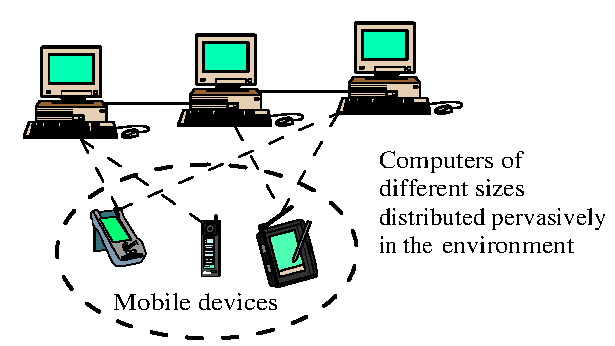
\includegraphics[width=7cm,height=!]{ch01/pm}
	\end{center}
	\caption{Pervasive and Mobile Devices}
	\label{fig:ch01pm}
\end{figure}

\begin{enumerate}[a.]

\item The technology can be \textit{pervasive}, that is, the computers are extended and diffused throughout every part of the environment. In a pervasive environment, the computational resources will tend to be uniformly distributed among the objects. The objects will contain a combination of sensors, and / or \textit{embedded} computers, and communication capabilities with humans (interface) or other computers. The objects will look like autonomous individuals, and every object will have its own processing unit, where it autonomously keeps track of the surrounding environment. That is, each object should have its own computer, its own sensors, and its own (unique) ways to communicate with and affect the rest of the environment. Depending on the context \cite{schilit94contextaware}, that is, the object location in the environment \cite{hightower01survey}, each object will create its own unique understanding of the environment and its history, and decide how to affect the environment in the future. In practice, some global view of the environment, along with the distribution of computational resources, makes it possible to optimize the coordination of object reactions (better context management). At present, it is also cheaper and easier to spread only sensors and the communication hardware, e.g., using the \textit{smart dust} technology \cite{kahn99next,warneke01smart}, and keep some of the event processing centralized.

\item The technology can be \textit{mobile}, that is, not stationary but movable around the environment, usually in the form of a personal computing device, or a \textit{wearable} computer \cite{wearable.1998}. It is the interaction with a ubicom environment, where the \textit{mobile} view of the technology becomes important. Suitable forms of interaction are needed to control a ubicom environment \cite{tochi-millenium}. Computers create a virtual model of the environment and operate in this model. The real world events should be converted to this virtual model, used to modify the state of the virtual model, and then the virtual model changes should be converted back to events than affect the real world. Human communication with a ubicom environment is part of this translation of the real world events.

Mobile devices offer convenient and suitable ways to map human interactions in a ubiquitous environment and are often an integral part of ubicom scenarios. Using a mobile device is simpler that moving to reach a touch screen nearby. There is no need to stay in a queue to use a mobile device, as it would be the case with a shared device when there are other people in the same place. Using mobile devices for interaction, also does not conflict with using other forms of communication, e.g., voice and gestures, but can be used to augment them.
%
There are also several other reasons why mobile computing and mobile applications are important for achieving ubiquitous computing. 

The non-uniform distribution of technology is likely to prevail. Not all environments will be equipped in the same ways. A mobile device that people can carry with, is a constant factor to rely upon, when designing applications in a non-uniform ubicom environment. It is cheaper to carry the technology around (e.g., a mobile phone), rather than replicate it in every corner (e.g., a public telephone cell every two meters). Even if a completely pervasive view of technology becomes possible and uniformly distributed, the mobile alternative pollutes the environment less with technology. Last but not least, a mobile device is a form of personal possession that can be carried always with. It may be used even if no networking is present. It makes sense to store data in a mobile device which are very personal, but difficult to remember, e.g., encrypted lists of passwords, financial records, and software that may be continuously needed.

Mobile phones were the first mobile devices to have global success and wide acceptance. Based on this success, there is a trend to enrich the number of services that are offered to people via mobile phones, benefiting from an extensive existing user base. The demand for more functionality is followed by a competitive supply of better hardware \cite{j2me.2005} and software for mobile devices. 
Mobile phones and mobile computers (Personal Device Assistants - PDAs) are becoming more powerful for less physical space. Both classes of devices are converging to a single device that has a telecommunication (networking) function and also serves as a personal computer device. This has opened a profitable market for third-party software for mobile devices supported by several platforms, e.g., J2ME \cite{www.j2me}, .NET CF \cite{dnetcf}, and BREW \cite{brew}, as well as frameworks \cite{ubi.infra.survey}, followed by a need for more applications that should be delivered in time. 

\end{enumerate}

%\subsection{Product-Lines for Mobile Device Software}
% The increasingly powerful mobile devices raise the need for more software specialized and optimized to run on them. It may seem that the restrictions in the processing power and other characteristic capabilities that mobile devices have currently, compared to desktop computers, are only temporary. However, there will be always restrictions on what can be done with a mobile device, compared to other more powerful contemporary devices, e.g., desktop PC-s.  

\section{Automating Mobile Software Development}

Mobile devices and their applications play an important and increasing role in ubiquitous computing. There are several non-functional ubicom challenges \cite{design.ubicom.2002} related to software infrastructure, e.g., the way to build and organize the application functionality, seamless migration of logic among devices and different environments, device software modeling, and scalability of the solutions.
To address these issues, the status of mobile software development needs to change from a craft, employed in a case by case manner, to a fully automated \textit{product-line} specialized for mobile applications. A product-line offers the possibility to reuse in the future the common investment done in a series of individual products \cite{Parnas.pl.96,pl.02}.

Mobile device applications share a lot of common non-functional features, e.g., screen management and data persistence\footnote{Preservation of the data, this is, the ability to store and load back the stored data.}, that can be factored out and made part of an automated product-line. The common functionality can then be requested declaratively and injected automatically in particular mobile device applications. Maximum automation can be achieved by focusing on a mobile application domain, and developing technology that takes into consideration the specific characteristics of the domain\footnote{A \textit{domain} is a specialized body of knowledge, an area of expertise, or a collection of related functionality \cite{pl.02}.}. Mobile applications are easier to automate than their desktop or server counterparts, because they have limited variability, e.g., in the ways the user interface is composed, or in the possibilities available for data persistence. Despite the advances in hardware technology, there is a set of properties that remain specific for mobile software, e.g., the limited screen size, low memory usage, sporadic networking, and ease of use, that need to be specially addressed. 

\begin{figure}[ht]
	\begin{center}
		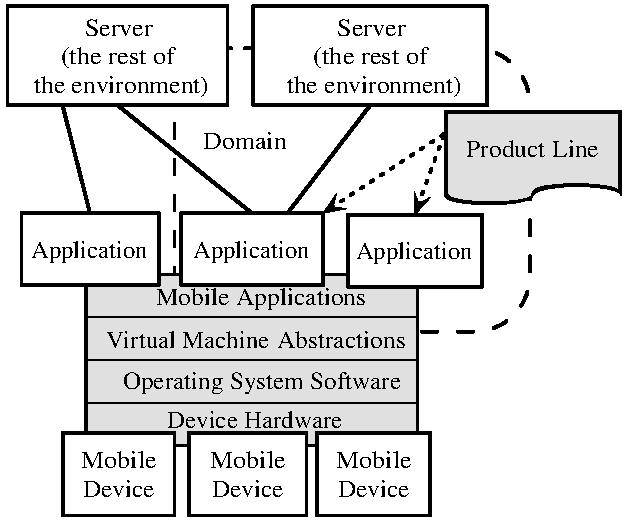
\includegraphics[width=10cm,height=!]{ch01/mobiledomain}
	\end{center}
	\caption{Mobile Device Applications Domain}
	\label{fig:ch01domain}
\end{figure}

At the software application level, isolation from specific mobile device hardware and specific operating system software can be achieved by using virtual machine abstractions, e.g., J2ME Mobile Information Device Profile (MIDP) \cite{www.j2me} and .NET Compact Framework \cite{dnetcf}. The focus in this book is in the domain of mobile applications that run on mobile devices supported by \textit{virtual machine} abstractions (\fig{fig:ch01domain}). As shown in \fig{fig:ch01domain}, several related mobile device applications can be managed by a product-line that addresses common repetitive technical issues. In a ubiquitous environment a mobile application also communicates with the environment as a client of one or more services, e.g., to access data in a central server-side location. Part of the server-side software found in the environment is closely related to the functionality of mobile device applications and may not be needed for other types of clients. This server-side part is represented inside the dashed box in \fig{fig:ch01domain}. It contains also repetitive technical concerns that need to be addressed by the product-line. A systematic and automatic approach for mobile application software development that addresses both client- and server-side issues is required. 

\subsection{Programming Models for Mobile Software}
\label{mobile.models}

Mobile and especially embedded software has been always difficult to write and debug for several reasons. There is a gap between the machine where the software is developed, usually a desktop PC machine, and the actual device on which the software will run. This gap requires using various emulators for the actual devices in order to build and test the actual software. One more step, namely emulator testing and (remote) debugging, is added to the usual development cycle of desktop software. Various implicit coding conversions, based on the language or specific API\footnote{Application Programming Interface.} restrictions, must also be followed in order to write efficient software.

\begin{figure}[ht]
	\begin{center}
		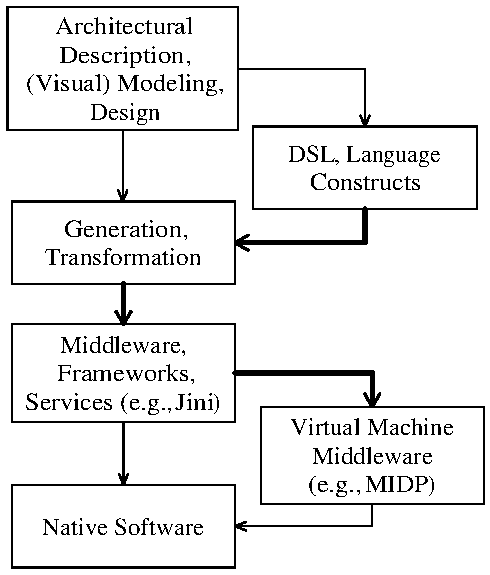
\includegraphics[width=7cm,height=!]{ch02/pm}
	\end{center}
	\caption{Programming Models for Mobile Software}
	\label{fig:pm}
\end{figure}

\fig{fig:pm} shows a high-level view of the common techniques used to develop software for small devices, such as, visual modeling and domain-specific languages (DSL) \cite{deursenetal.00}. Programming small devices can start at any node of the diagram in \fig{fig:pm}. Not all systems use all the paths shown, and more than one path is possible. For example, the model of an application can be defined by using visual domain abstractions. This visual model is then either converted to a specific DSL, or is used to generate directly source code in a general-purpose language. The generated code targets directly the native software, or makes use of existing middleware frameworks. The application could run against the device hardware, or on the top of a virtual machine. Various forms of these programming models have been used in real-time embedded systems \cite{realtime.77,ghosh94survey,emb.gen.02}, and other embedded software and frameworks \cite{BurchPasseroneSangiovanni-Vincentelli2001,emb.comp.03}.

Mobile device applications addressed in this book have less restrictive requirements than embedded systems, but more restrictions than other PC desktop software. Virtual machines, e.g., J2ME \cite{www.j2me}, .NET CF \cite{dnetcf}, and their programming models, such as MIDP \cite{www.midp-ota}, help to hide the hardware and software details for different classes of mobile devices. Virtual machines, however, do not offer high-level abstractions for application domains. As the focus on ubiquitous computing grows, so does the number of mobile applications that need to be developed and debugged. There are more and more applications for mobile devices that share a lot of similarities, but also have their own peculiarities. Reusing only the virtual machine abstractions to hide OEM\footnote{Original Equipment Manufacturer.} specific device details is not sufficient any more. The commonality and variability of families of applications must be supported as well.

More than one programming abstraction of \fig{fig:pm}, e.g., visual modeling, DSL and code generation, can be used to factor out and reuse the common functionality, and some of them are more declarative than the others. The approach presented in this book goes along the bold connection lines in the \fig{fig:pm}. The goal is not to develop a new kind of middleware system, but rather to propose ways that automate the creation of third-party mobile software by relying on existing middleware, such as MIDP \cite{www.midp-ota}. MIDP application development can be supported with abstractions that organize and reuse MIDP specific domain functionality. The interest will be in declarative representation of the domain abstractions at the source code level. Declarative constructs preserve the domain abstractions in the source code, and reduce the development and debugging time by hiding the details of a more complex underlying programming model.

\subsection{Variation Mechanisms for Mobile Application Product-Lines}

There are different ways to parameterize the common behavior characterizing a domain and reuse it in a specific application, known also as \textit{variation mechanisms} \cite{pl.00}. The automation of mobile device software product-lines requires generic software technology to support \textit{iterative} \see{sec.iterative.pl} product-line development. This means that the variation mechanisms should be:
\begin{enumerate}[a.]
\item Easy to introduce and maintain (low-cost). The iterative development of a product-line is important to support product-line evolution \cite{Pussinen.2002}.  
\item Flexible to support design experimentation. The correct \textit{domain abstractions} used to represent the \textit{domain concerns} are often not completely known from the beginning and may change as the product-line evolves.
\item Declaratively supported to reduce accidental complexity \cite{brooks.87} and achieve transparent automation.
%
The domain dependent concerns should be injected automatically in a specific mobile application. Domain dependent concerns are code-related \textit{core assets} (reusable artifacts) for a domain \cite{pl.02}. 
\item Enable a clear separation of the common domain functionality and the application specific functionality and enable domain-specific optimizations. The domain concerns are usually \textit{cross-cutting} \cite{kiczalesetal.97}, that is, they are needed in more than one place (components) within an application.
\end{enumerate}

Several technologies \cite{pl.00} can be used to support variation, e.g., inheritance, component libraries (object-frameworks \cite{batoryetal.00}),
extensions (selection of variants), configuration,
parameterization, templates, macros,
generation \cite{generative.00},
(embedded) domain-specific languages (DSL) \cite{deursenetal.00}, compiler directives,
visual modeling and CASE\footnote{Computer Aided Software Engineering.} tools. All these variation mechanisms have their own benefits and drawbacks and need to be specifically evaluated for mobile software applications.
%
The library solution is the simplest one, as it requires no further tool support other than those offered by the development language. It offers minimal automation for inserting the domain concerns into an application. Code generation is easy to implement, but pure generative solutions\footnote{That is, generative techniques used alone, not in a combination with other variation mechanisms.} are difficult to maintain and debug because of the programming indirection and lack of early static checking.
DSL are more declarative and enable transparent automation, but have high start-up costs to be implemented. 
Visual modeling abstracts the domain concerns, but it does not support well iterative development of abstractions and traceability. Often it is not feasible to define every piece of behavior visually and source code artifacts are used instead\footnote{For example, a UML-based CASE tool may generate only code stubs, whereas the method internals need to be filled out manually. The functionality of the methods could also be specified visually, but unless the functionality is made of well-known repetitive code, it is often easier to program using source code directly.}. A more elaborated discussion of the variation mechanisms of interest for mobile product-lines is provided in \sr{c2sec:pline}.

\section{Attribute Enabled Software Development}

This book introduces variation mechanism that fulfills the requirements posed for mobile product-lines and does not have the problems encountered with other variability mechanisms. Mobile software product-lines can be implemented with programmable software container abstractions, backed up at the source code by lightweight domain-specific abstractions, encoded as explicit code attributes, which are interpreted by means of code transformation techniques. This section explains shortly what is meant by these terms.

\subsection{Mobile Containers}

A \textit{software container} is an architectural abstraction that can be used to organize a product-line for a domain, by factoring out the common domain behavior into a set of \textit{services} provided by the container. The container services are reused by all applications in the product-line. An application component inherits quasi-transparently the domain-wide features from the container it is deployed in. That is, when developing an application, the developer can focus exclusively on the features that are specific for the particular application at hand. The domain concerns are provided (\textit{injected}) when needed, into the components of the application by the container implementation. 

The container abstraction is known from enterprise server-side containers, e.g., COM+ \cite{comp.services} and EJB \cite{j2ee14}. The idea can be applied to organize services in every domain of interest, especially to achieve automation of a mobile product-line. The container creates a well-defined boundary between the domain abstractions and the rest of an application. For a mobile application, the container provides a single centralized point of maintenance, that wraps the underlying services offered by the middleware (e.g., J2ME \cite{www.j2me}), making it easier to support mobile software evolution.

\begin{figure}[ht]
	\begin{center}
		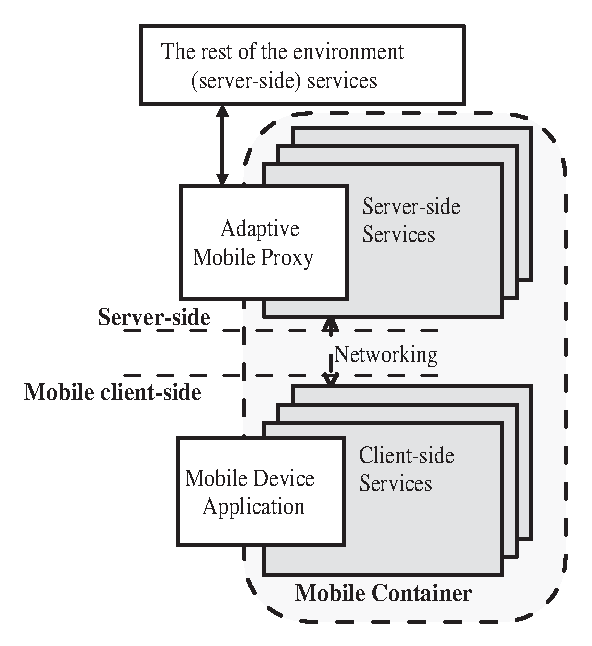
\includegraphics[width=8cm,height=!]{ch01/mobc}
	\end{center}
	\caption{Mobile Container Architecture}
	\label{fig:ch01mobc}
\end{figure}

The term \textit{mobile containers} will be used in this book to refer to a special combination of client and server containers which is appropriate to accommodate the specific characteristics of the domain of mobile applications. A mobile application is a client application with \textit{sporadic} network connectivity. As such, it is neither a thin nor a thick client\footnote{A thin client does only interface processing on the client-side and delegates any other data processing to the server-side. A thick client does most of the data processing on the client-side.}. It cannot be a thin client, because it should be able to do some processing and data storage on its own when disconnected. It cannot be a thick client either, because of the restricted resources of a mobile device. In order to save computing resources of the mobile device, as much of data processing as possible should happen on the server-side.

A distinction will be done between the server-side functionality that is specific for mobile device applications, and the functionality that is common for other types of clients\footnote{E.g., powerful desktop clients.}, as illustrated in \fig{fig:ch01mobc}. The server-side functionality that is common to mobile clients can be factored out from the rest of the server-side services in the form of an \textit{adaptive proxy} \cite{fox96adapting}. The mobile container is devised as a special kind of a software container \cite{server.patterns.02} that automates the organization and injection of domain concerns (a) in the mobile device client applications, shown in the lower part of \fig{fig:ch01mobc} and (b) in the intermediate application-level\footnote{Not to be confused with lower level proxies used to represent objects remotely over a network.} proxy part between the server (environment) services and the mobile clients. The adaptive proxy stands also on the server-side (\fig{fig:ch01mobc}). The server-part of a mobile container automates those aspects of the proxy that are directly connected with the functionality found on the mobile clients. It is the responsibility of the adaptive proxy to serve as a central connection point for representing the mobile clients and to communicate with the rest of the server-side services. The product-line handles the concerns of the both parts of the mobile container. 

To support the domain variability, the container itself should be \textit{programmable}, i.e., configurable, rather than providing a predefined set of services. The container can be used to inject any parameterized set of services into specific application components, using implicit or explicit architectural conventions. An open and extensible plug-in architecture with a configurable workflow is presented in this book \seec{ch05} to organize the product-line assets as container supported services. This enables software developers to specialize the product-line assets to fit their needs and to maintain them.

The inheritance of common properties from the environment is known as \textit{environmental acquisition} \cite{lorenz.96,ea.05} and could be supported by special language support. Some languages, e.g., Keris \cite{keris.04}, replace static linking with dynamic linking and can be used to support some form of environmental acquisition. The solution for modeling environmental acquisition presented in this book is \textit{lightweight} in the sense that, it can be  easily added to any existing language, making it suitable for iterative product-line development. The presented solution requires only a minimum extension to the existing language features, namely the ability to decorate the elements with attributes and support for interpreting the latter. The solution also makes the boundary between the application and the domain functionality explicit.

\subsection{Lightweight Domain-Specific Abstractions}

\textit{Domain-specific abstractions (DSA)} are language abstractions, usually in the form of embedded domain-specific languages (EDSL) \cite{kamin.98}, used to extend a general purpose programming language. DSA are used to add declarative support for specific concepts of a domain to a language, making it easer to write software for that specific domain. Having domain abstractions in code helps to preserve the domain architecture at the code level. The source code that contains the key abstractions of a domain declaratively is easier to understand. Declarative DSA blur the architectural gap \cite{sf.04} between a specific modeling step, and modeling directly at the source code level. DSA can be used to declaratively request the container-based services in the source code of a mobile application. As illustrated in \fig{fig:ch01dsaserv}, declarative DSA can be interpreted and automatically connected to the container provided services.


 %Thus, DSA reduce a step in debugging the final product-line code, rather than having, for example, to go though a visual modeling tool and refine the model. This is preferable, especially in the early stages of a product-line, when the final automation corresponding to the domain abstractions is not always quite clear. As the product-line development stabilizes, it is easy to introduce tool supported (visual) modeling for the domain based on the declarative DSA created.

\begin{figure}[ht]
	\begin{center}
		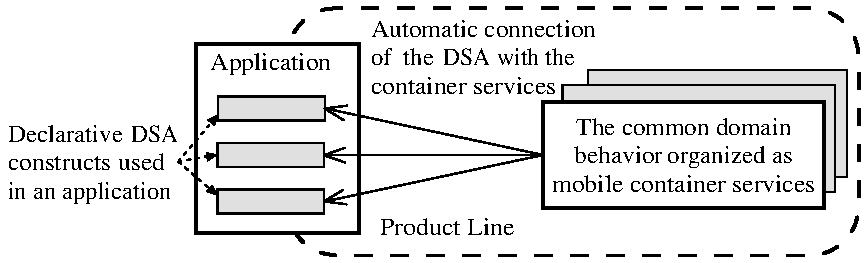
\includegraphics[width=12cm,height=!]{ch01/dsaserv}
	\end{center}
	\caption{Connecting DSA with the Container Services}
	\label{fig:ch01dsaserv}
\end{figure}

% Several abstractions may be needed to implement a container and to support its services. Such DSA should be easy to introduce and maintain.

Explicit attributes \cite{java.explicit.programming}, directly supported at language level, can be used as a low-cost mechanism to emulate DSA. Attributes\footnote{The terms \textit{attribute}, \textit{annotation}, and \textit{tag} will be used interchangeably to denote the same concept, unless explicitly noted otherwise.} are a lightweight language extension that remove the need to implement explicit domain specific language abstractions \cite{Taha.1997}. Attributes can be used as a variability mechanism to model product-line domain abstractions directly in the source code of a specific mobile application \see{attribute.families}. Attribute-based abstractions are cheap to introduce and to modify in a general-purpose language.
% and reduce the cost of introducing the domain abstractions.
 A language with support for attributes and attribute-driven transformations eliminates the need for other parsing and EDSL tools for implementing language abstractions to sustain mobile product-lines.

%The lightweight nature of attribute-based abstractions can be combined with generative \cite{generative.00} code techniques to enable domain-specific optimizations, for example to have a minimum level of abstraction layers. While attribute-based abstractions exist in the source code, they are treated as logical abstractions. That is, after attribute-based abstractions are interpreted / compiled, no further real abstraction layers are added to the system. For the programmer, however, the layers exist and could be used to reason about the system architecture of the domain.

Several general purpose language technologies, e.g., .NET \cite{www.dotnet} and Java \cite{www.java}, already offer some support for attributes. The main support provided by these technologies is to enrich structural entities, e.g., classes and methods, with attributes and to preserve such decorations in the binary meta-data\footnote{Data describing the other data.}. A more complete support for attributes and attribute transformations as part of the language technology is needed when attributes are used to emulate DSA. The abstract syntax tree (AST) created for the source code internally by the compiler, the AST-s created by various source processing tools (and API-s), and the AST obtained via reflection in languages that support meta-data, represent similar views of the same data structure, at various levels of detail\footnote{For example, the details of the method body are not modeled in the reflection API.}. The interfaces used to model these similar AST views are often different and the transformations done in one view are not easy portable to another view.

It is possible to unify all different AST representations, in a single data structure that provides support for different levels of detail. This generalized AST can be obtained either from source code or binary data, and can be used to implement attribute transformations for mobile product-lines. For attribute languages, this common representation will be called a \textit{Generalized and Annotated AST (GAAST)}, and the languages that offer such an API as part of their technology will be called \textit{GAAST languages}. The GAAST API, combined with ways to enable filtering nodes of interests, can be used as a common API to implement meta-programming attribute-driven transformations in a general-purpose language. If GAAST is part of the language, the investment on the transformation tools is protected as the language evolves.

Attribute enabled languages affect also the design \cite{design.attrib} process. OMG Model-Driven Architecture (MDA) \cite{mda.frankel} transformations, whose input models are represented as UML\footnote{Unified Modeling Language.} class diagrams, can be directly supported in a GAAST language. Using attributes to sustain DSA at the language level preserves architectural decisions of the domain models. GAAST languages require only type mappings to support several MDA Meta-Object Facility transformations. In MDA, the software development could start with a platform independent model (PIM), and then be iterated toward a platform specific model (PSM), introducing platform specific details in each step. GAAST languages offer a common API to directly support such transformations and open new possibilities to design applications, that will be investigated in detail in \kr{ch03}. 

\subsection{Attribute-Driven Transformations}

Any invasive \cite{java.compost} system that can access the abstract syntax tree (AST) of a program can be used to implement static attribute-driven transformations for attribute-based DSA in a product-line. For example, GAAST languages offer all the necessary means to support attribute-based transformations. The implementation of transformers in the GAAST API level is still very general, and may result in non-reusable transformers which are difficult to maintain.

Programming at the GAAST-level requires following implicit coding rules to be able to reuse the transformation behavior. Many AST manipulations based on the GAAST-API are repetitive across different transformation operations. Transformer implementations that directly build upon GAAST lack a clear structure of the transformation process. This opens the need for specialized transformer technology to enforce reusable modular organization of attribute-based transformers. Having modular transformers facilitates understanding the attribute semantics, and helps using attributes successfully to model the domain variability.

\begin{figure}[ht]
	\begin{center}
		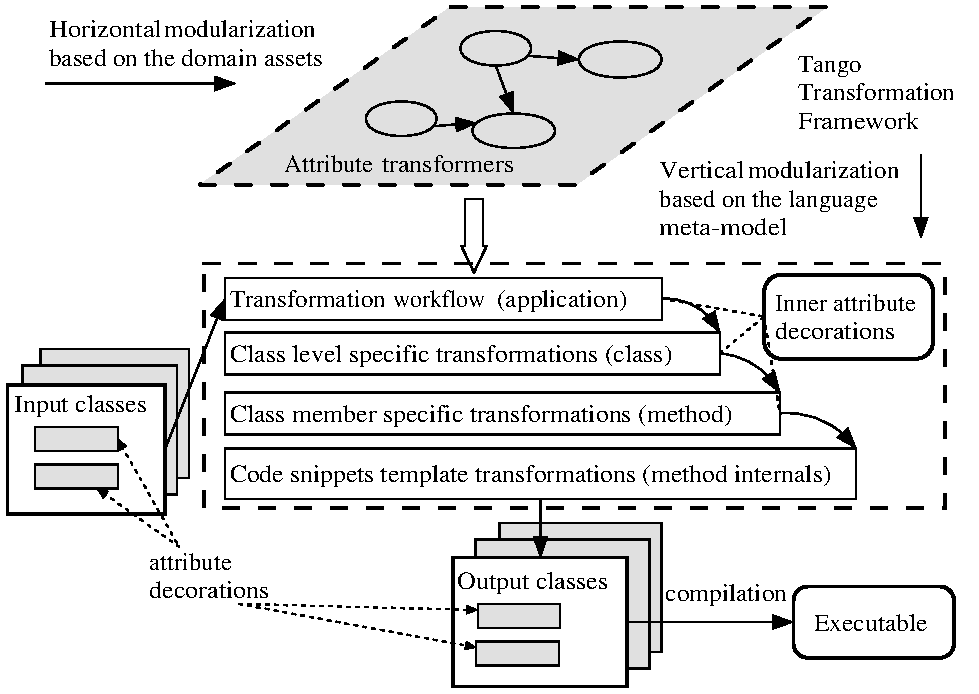
\includegraphics[width=15cm,height=!]{ch01/tango}
	\end{center}
	\caption{Layered Attribute-Driven Transformations}
	\label{fig:ch01tango}
\end{figure}

Knowledge about the domain, modeled as a set of attribute-based DSA, and about the deployed programming language can be explored to introduce a \textit{horizontal} and \textit{vertical} modularization for attribute-driven transformers (\fig{fig:ch01tango}). The transformation process can be structured horizontally according to the domain assets modeled with attribute-based DSA. The knowledge about the specific domain assets can be used to guide the transformation workflow. The workflow dependency graph can be partially computed automatically, based on local \textit{before} and \textit{after} dependency relations supplied by the developers that model the semantics of the interactions between the domain assets.

Knowledge about the structural nesting of the elements found in the language meta-model can be explored to organize the transformation strategy in vertical layers, as shown in the middle part of \fig{fig:ch01tango}. The approach for modular construction of attribute-based transformations taken in this book, embodied into the Tango transformation framework \seec{ch04}, supports a hardwired common OO language meta-model made of classes, fields, and methods, which in turn are made up of method code blocks. The hardwired meta-model enables a vertical layering that otherwise would not be possible with an arbitrary open meta-model. Some other frameworks \cite{stratego.01,www.aspectjt} deal with this issue by defining parameterized transformation operations, e.g., selection and iteration, that can work with any AST element type, but have a single layer to organize the transformation process. The approach presented in this book defines also declarative operations, but specializes them for each meta-model element type and organizes them in layers according to the language meta-model. The transformation process in Tango shown in \fig{fig:ch01tango} contains operations specialized for each transformation layer, e,g., class level specific operations. %This modularization can be automatically enforced.

%Splitting the transformation strategy allows to organize the transformer implementation into a series of layers. Each layer is only allowed to create transformers for elements of the lower layer, and delegates to them to carry out the exact details of the transformation. Furthermore, a layered transformation strategy enables reuse. The lower layer transformers focus in small atomic tasks and could be reused in more than one upper-level transformation. Organizing the transformation process in several stages \cite{Taha.1997} enables a high-level view of the transformation process and divides understanding what a transformer does at various levels of detail\footnote{Understanding what a transformer does often stops without the need to see what low-level layers do.}. Layering serves also to document the semantics of the set of attributes upon which a specific transformer works and helps to support transformation traceability.

Attribute-based transformers do not only operate on AST nodes that are explicitly decorated with attributes, they can also decorate the AST as they process it with \textit{inner attributes}, intended to support the transformation process (schematically shown in the middle right part of \fig{fig:ch01tango}). This technique is similar to saving the intermediate transformation results into declarative placeholders \cite{asfsdf.02}. Unlike in a compiler, where the AST decoration with attributes is used only internally \cite{java.compilers.book}, attribute-driven transformers treat the explicit\footnote{Attributes used in source-code directly to express the DSA semantics.} and the inner attributes\footnote{Attributes that express internal transformation semantics.} uniformly. Given an attribute, a transformer cannot tell whether it comes from the source code, or from another previous transformer. 

Inner attributes enable a declarative composition of transformers. A transformer declares (a) the set of attributes that it expects the AST elements to have, and (b) the set of attributes the elements will have after the transformation. Without relying on attributes for coupling transformers in a chain, each transformer needs to re-check all properties of the AST elements passed to it, before it processes them. When using attribute-based coupling, the transformers can rely on attribute decorations of previous transformers and do not need to revalidate all the semantics the input units are required to have. 

Some attribute-driven transformer operations, e.g., checking attribute dependencies, are generic and can be factored out of any transformer. Such cross-cutting transformation concerns can be made declarative by using a way that is natural for GAAST languages. The decoration of an attribute with other attributes (often called \textit{meta-attributes}) can be used to declaratively express generic operation semantics, e.g., the attribute dependencies. In the attribute dependency case, presented in \kr{ch04}, attributes are decorated with appropriate forms of a dependency attribute when they are created. Decorated attributes can be used as normal attributes. The dependency information can be later checked and enforced automatically depending on the attribute usage context.

\Kr{ch04} explains how the mechanics of this proposal for organizing attribute-driven transformations can be made declarative and automatically enforced, by creating a language specialized for attribute-based transformers. Such a language makes the transformation operations more declarative and easier to write and maintain.   

\section{Contributions of this Book}

Most of the contributions of this book are specific for mobile software and mobile software product-lines. Other contributions are of generic nature, and apply also to product-lines for other domains. This section only briefly mentions the introduced concepts to organize them in a single place. For more information see the referred chapters.

\noindent \textbf{Architectural Contributions}
\begin{itemize}

\item This book contributes a new architectural style for organizing the domain assets of a product-line as \textit{container-managed services}, based on \textit{attribute enabled software development}. An open container supported by attribute-based DSA can be easily extended with new services that model the domain concerns supporting iterative product-line evolution \seecc{ch02}{ch05}.

\item A new kind of container abstraction for mobile product-lines, a \textit{hybrid mobile container}, is another contribution. A mobile container is a unique combination of a client and a server container, optimized to automate product-lines for mobile device software. An enterprise server-based container extends from server to client \cite{server.patterns.02}. The reverse is true for a mobile container. The mobile container represents a client extension on the server-side, and takes over some operations normally handled by a client application and moves them to the server-side \seec{ch05}.
\end{itemize}

\noindent \textbf{Language Contributions}
\begin{itemize}

\item This book contributes the notion of \textit{Generalized and Annotated AST (GAAST) languages} used to unify common AST related API-s, supported by the language technology, to enable uniform source and binary transformations. GAAST creates a low-cost language workbench \cite{lang.workbench} to support attribute-based DSA. As various transformation techniques are being continuously explored, having a unified mechanism for transformations as part of a language reduces the cost of building and maintaining several third-party tools \seec{ch03}.

\item The book helps to bridge the gap \cite{sf.04} between modeling and coding, by relying on \textit{architectural support via low-cost DSA}. DSA preserve the architecture of product-line domain assets directly in source code. Low-cost attribute-based DSA make it possible to directly utilize the product-line domain abstractions at the language level \seec{ch03}.

\item This book also contributes to the domain of specialized languages for \textit{attribute transformations}. Attribute transformation languages serve as domain-specific languages for attribute transformations that enforce modularity and enhance reuse \seec{ch04}. These languages make use of the characteristics of the addressed domain to enable better organization of the transformation process, increase productivity, and automate traceability. 
\end{itemize}

\noindent \textbf{Transformation Contributions}
\begin{itemize}
\item \textit{Specialized attribute transformation engines} are introduced as a technique to support attribute-based DSA transformations in the context of a mobile container. Specialized attribute transformation engines are organized as a series of transformation layers. Inner attribute decorations make attribute transformer coupling declarative and enable transformer composition \seec{ch04}.

\item Another contribution is the enhancement of the \textit{attribute transformation support with meta-attributes}. Attribute transformation concerns that cross-cut more than one transformer can be addressed declarative by expressing them as meta-attributes. Meta-attributes are used to extend an attribute enabled language, to support generic transformation operations, e.g., attribute dependency. Such generic operations are made native to a GAAST language by organizing them as meta-attribute decorations over the attribute definitions \seec{ch04}. %This is a natural and generic way to extend attribute and attribute transformations support in the GAAST languages.
\end{itemize}

\noindent In addition, several \textbf{practical contributions} have resulted from the concrete instantiations of the conceptual contributions:

\begin{itemize}
\item The \textit{MobCon} framework \cite{cepa.mezini.hicss38} is a mobile container for J2ME MIDP \cite{www.midp-ota}. Several MIDP concerns are addressed and organized as a generative mobile container framework based on the technology developed in this work \seec{ch05}.

\item The \textit{MobCon Transformation Engine (MTE)} is a generative GAAST-based transformation engine for Java. The generative attribute transformation engine of MobCon is extensible, and can be used to implement Java-based attribute containers for other domains apart of the J2ME MIDP \seec{ch05}.

\item The \textit{Tango} framework \cite{cepa.tango.ICSR8} is an attribute-based transformation language. Tango is a prototype implementation of layered attribute transformers with inner attribute notations. Tango enforces layering of the transformation process and offers transformation predicates specialized for each meta-level \seec{ch04}.

\item The \textit{Attribute Dependency Checker (ADC)} \cite{cepa.mezini.gpce.04} is a constrain checking engine for .NET attribute dependencies \cite{www.dotnet}. ADC makes use of meta-attributes to declare attribute dependencies for any depth level of the structural tree, and to enforce them automatically \seec{ch04}.

\end{itemize}

\section{The Structure of the Book}

\Kr{ch02} provides background information about current technology for software product-lines. Product-lines and various variability mechanisms are discussed. The container abstraction is presented and an overview of invasive and non-invasive container implementation techniques is given. In the end, aspect-oriented techniques are compared with more specialized transformations.

\Kr{ch03} focuses on attribute enabled software development (AESD). The architectural properties of attribute enabled languages are presented by a Model-Driven Architecture (MDA) transformation case study, where the same model is mapped using representative ways onto language constructs. An overview of attribute support in .NET is given, followed by a generalization of these ideas in the form of a GAAST language. Next, a comparison of GAAST languages and other meta-programming approaches is made. The chapter ends with some heuristics about the right usage of attributes.

Attribute-driven transformations, and specialized languages to support them, are the theme of \kr{ch04}. Different ways to make the attribute-based transformations modular  are explored. The focus will be on the Tango language, specialized for attribute-driven transformers. Tango enforces a layered structure upon the transformer implementations. A declarative way to represent and enforce attribute dependencies based on meta-attributes is discussed in the end.

\Kr{ch05} builds upon the concepts of the previous chapters, and shows how a mobile container for Java 2 Micro Edition - Mobile Information Device Profile (J2ME MIDP) can be constructed. The GAAST ideas are used to develop a generative container framework for Java, and specialize it with services that are specific for MIDP applications, such as, data persistence, image adaptation, and user interface management. A medical application for X-Ray diagnostics is used to demonstrate the usefulness of the developed MIDP container framework.

\Kr{ch06} provides a summary of the main concepts and presents some ideas for future work. The related work is distributed uniformly in every chapter, to keep it near the point where the relevant technical details are discussed. 

Most of the material presented in this book shares content with several conference and journal publications of the author which are referred to in the corresponding chapters.
%ch02.tex

%\pagestyle{myheadings}
%\markboth{\chaptermark PROBLEM STATEMENT }{\rightmark }
%\markboth{ \chaptermark PROBLEM STATEMENT}{ \sectionmark }

\chapter{Organizing Mobile Product-Lines with Mobile Containers}
\label{ch02}
\mquote{The harder is to see the design in code, the harder is to preserve it, and the more rapidly it decays.}{M. Fowler, Refactoring - Improving the Design of Existing Code, Addison-Wesley, 1999}
%He is saving by
%doing things only once - The Imperial Chronicle, Volume II, Issue II, Page 2, 2000, ecs-imperial.org
%People are good for doing things only once - Fritz Scheuren}

%On other hand
%we
%further mode
%however
%one
%also

\noindent This chapter serves two purposes:
\begin{itemize}
\item It introduces background information needed to explaining several technologies discussed in this book. Details are given about product-lines, variability mechanisms, software containers and their implementation techniques.

\item It provides an extended overview of the software issues and problems addressed in this book. The focus is on automated product-lines with language support for domain abstractions. The material presented in this chapter serves as a starting point for the upcoming chapters.

\end{itemize}

While most of the information discussed in this chapter is also relevant for other domains, the focus will be on the importance of such technologies for supporting product-lines for mobile device software. This chapter is organized as shown in the Figure below.

\begin{figure}[ht]
%	\begin{center}
	  \xymatrix{
	  *+[F]{\txt{Product-Lines for Mobile Software \\\Sr{c2sec:pline}}} \ar[dr] \ar[d] & \\  	
	  	*+[F]{\txt{Software Containers  \\\Sr{c2sec:containers}}} \ar[d] & *+[F]{\txt{Domain-Specific Abstractions \\\Sr{sec:var.dsa}}} \ar[d] \\  	
	  	*+[F]{\txt{Container Implementation Techniques \\\Sr{c2sec:implement}}} \ar[r] & *+[F]{\txt{Aspect-Oriented Programming \\\Sr{ch2:aop}}} \\	  	
	  }
%	\end{center}
%	\caption{Chapter Overview}
%	\label{fig:contents}
\end{figure}

%\Sr{mobile.models} starts with a short introduction of programming model for software development for mobile devices, focusing on using virtual machines to hide device hardware and original equipment manufacturer (OEM for short) software details and explaining the direction followed in this thesis.

\Sr{c2sec:pline} justifies the need for bringing in more automation in the development of mobile software by employing product-lines. The preferred characteristics of a product-line for mobile applications are given in \sr{sec:var.mob.pl}. The section compares several variability mechanism focusing on object-oriented frameworks, visual modeling with Computer Aided Software Engineering (CASE) tools and domain-specific languages \see{sec:var.dsa}. 

Software containers represent an architectural pattern of interest that can be used to organize mobile product-lines. Containers transparently introduce functionality into a set of serviced components. The container abstraction is known from technologies, such as, EJB and COM+. An overview of these two technologies and how they use containers, is given in \sr{c2sec:containers}. The benefits of generalizing the container concept as a means to automate arbitrary domains are then explained.

\Sr{c2sec:implement} addresses several technical issues related to implementation of the container abstraction. Background information about various possible implementation technologies is given, making a distinction between invasive and non-invasive transformations. These technologies are used to sustain programmable dependency injections, separating the serviced components from the container services. Invasive and non-invasive techniques are evaluated for mobile containers.

Aspect-oriented programming (AOP) techniques are compared with other invasive techniques for implementing domain-specific abstractions (DSA) in \sr{ch2:aop}. \Sr{ch2sum} ends this chapter with a summary and an overview of the proposed technology.

\section{Reusability with Product-Lines}
\label{c2sec:pline}

Factoring out the common functionality of mobile software and reusing it in specific mo\-bi\-le appli\-ca\-tions can be done with automated \textit{product-lines} \cite{Parnas.pl.96} specialized for mobile applications.
%
A software product-line is defined in \cite{pl.02} as \textit{"a set of software-intensive systems sharing a common, managed set of features that satisfy the specific needs of a particular market segment or mission and that are developed from a common set of core assets in a prescribed way"}. Other terms used often interchangeably to describe product-lines are \textit{product (application) families} \cite{Parnas.pl.96,pf.00} and \textit{software factories} \cite{sf.04}. This section gives an overview of product-lines and discusses several mechanisms of interest for implementing product-lines that automate mobile software. %Our treatment of product-lines here is based mainly on \cite{pl.02,harsu.2001,Pussinen.2002}.

\subsection{Two Views of Product-Line Development}
\label{sec.iterative.pl}

A product-line reflects the experience gained by creating many applications that share some common set of characteristics, usually because they belong to the same domain. This common set of characteristics can be parameterized and can be factored out to represent the domain variability. This is also known as \textit{variation management} \cite{harsu.2001}. The common functionality is reused \cite{pl.levels.00} in every new application within the same domain. \textit{Application families} \cite{pf.00,Parnas.pl.96} are made up of several applications that share the reusable functionality provided by the product-line. 

\begin{figure}[ht]
	\begin{center}
		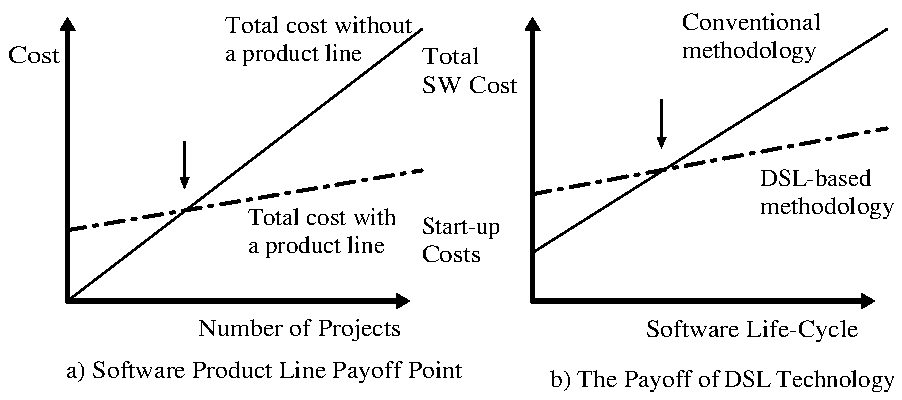
\includegraphics[width=12cm,height=!]{ch02/pl-cost}
	\end{center}
	\caption{Product-Line Payoff}
	\label{fig:pl-cost}
\end{figure}

\begin{figure}[ht]
	\begin{center}
		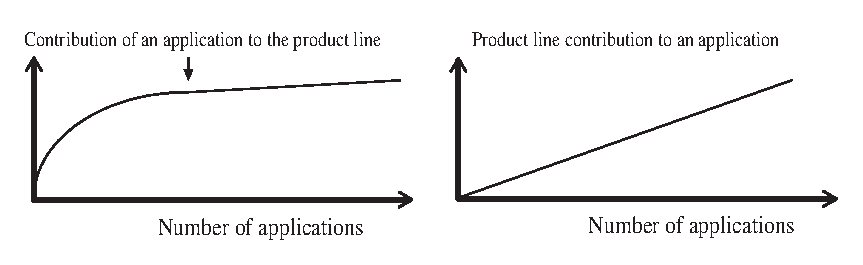
\includegraphics[width=11cm,height=!]{ch02/productline}
	\end{center}
	\caption{A Product-Line and its Applications}
	\label{fig:productline}
\end{figure}

A product-line can be seen as up-front investment that pays itself off in the long term. This is showed often graphically as in case (a) of \fig{fig:pl-cost}, taken from \cite{pl.02}, where the start-up costs of the product-line approach are bigger than those of an approach without a product-line. The product-line investment pays off after a given point. These empirical diagrams look similar for other technologies that require some up-front investment as in case (b) of \fig{fig:pl-cost} that shows the payoff for domain-specific languages (DSL), taken from \cite{hudak98modular}.

An alternative view of a product-line is to consider it as an accumulation of investment, rather than an up-front investment. The more similar applications are built for a given domain, the more the previously implemented functionality will be reused in the new applications. Turning such an accumulation of investment into a really profitable product-line is a matter of discipline and architectural refactoring \cite{refactor.99,sf.04}. There is a mutual contribution between the product-line and a specific application illustrated by the diagrams of \fig{fig:productline}: (a) each specific application contributes (back) to the product-line, enhancing its variability; (b) the factored common product-line functionality is reused with proper variability parameters in a specific application implementation. A product-line is in an iterative development process, while new applications are created for the same family. In the long term, it is expected that after a \textit{threshold} point, the product-line development changes very slowly when new applications are created. The threshold point is envisioned to be very close to the payoff point of the up-front investment view of product-lines.

The iterative view of a product-line is more suitable than the up-front investment view for the domain of mobile device software. Each ubiquitous computing scenario has its own peculiarities and contributes back in the common code base that is shared between all mobile applications, which are based on the same set of technologies for a given domain. The product-line assets are gradually structured as more scenarios are implemented.

\subsection{Variation Mechanisms for Mobile Product-Lines}
\label{sec:var.mob.pl}

The common functionality of mobile applications can be reused when it is parameterized with regard to its variability. There are different mechanisms for organizing and reusing the common product-line functionality, known as \textit{variation mechanisms} \cite{pl.00,harsu.2001}, e.g., component libraries, inheritance and code generation. From the point of view of an iterative approach to mobile software product-line development and evolution, three general requirements can be identified. Some of these requirement are useful for any kind of software product-line, however, they are especially important for mobile applications. 

\begin{itemize}
\item The variation mechanisms for mobile product-lines should \textit{facilitate the introduction and maintenance of domain abstractions.} The creation of a product-line is an iterative process. It should be easy to start creating a product-line, adding functionality to it at any time and maintaining it. No product-line is acceptable unless it can deliver in time \cite{sf.04}. If the costs of introducing reusable assets in a mobile product-line are high, the product-line will not be embraced in the early phases of the development. This will make it even more difficult to introduce a product-line later on, after some applications have been developed. The variation mechanisms should enable the evolution of the domain assets, as the underlying mobile technology (middleware) changes often, to respond to the market demands and technology innovations.

\item The variation mechanisms for mobile product-lines should \textit{enable stating declaratively and introducing automatically the domain functionality.} The integration of the product-line's generic functionality into a specific mobile application should be as much automated as possible. Automation accelerates the time to market, by reducing the debugging time (which is higher for mobile applications because of the indirection gap between the machine where the development is made and the device where the software runs).

The used variation mechanisms should enable a declarative representation of domain assets, in order to preserve the design model within an application, and to avoid accidental complexity \cite{brooks.87}. Declarative constructs are important to ease the maintenance of a product-line during its evolution \cite{Pussinen.2002}, and to clearly define the boundary between the generic domain functionality and the application specific functionality.
%
As noted in the discussion of case (a) of \fig{fig:pl-cost}, the product-line start-up costs are usually higher than the costs of applications without a product-line. Adding the costs of developing a declarative notation (case b), to the product-line start-up costs related to domain engineering, can result in an unacceptable overall cost for a project. As argued in \cite{hudak98modular}, it is not sure that the payoff point really comes in every case. Hence, declarative variation mechanisms with very low start-up costs are needed.

\item The variation mechanisms for mobile product-lines should \textit{enable domain-specific optimizations.} Mechanisms that balance between the increased level of abstraction and the introduced run-time performance are needed. For example, the indirection layers could be minimized. For example, in the J2ME MIDP \cite{www.j2me}, the class meta-data are saved in the application's binary file. The number of classes affects the size of the application and should be kept in a minimum.

\end{itemize}

\noindent To summarize, the variation mechanisms (VMs) for product-lines for mobile applications should:
\begin{enumerate}[a.]
\item make the domain functionality explicit by means of declarative domain specific abstractions,
\item provide for stability of domain abstractions in the prospect of fast underlying technology changes,
\item support automated integration of domain and application functionality,
\item have low start-up costs and require minimal additional (language) technology,
\item enable domain-specific optimizations.
\end{enumerate}

\Kr{ch01} listed several variation mechanisms for product-lines discussed in \cite{pl.levels.00,pl.00,harsu.2001}, e.g., inheritance, code generation, and compiler directives. An overview of the other techniques can be found in \cite{sf.04}. The list of the variation mechanisms given in \cite{pl.levels.00,pl.00,harsu.2001} is extended in this section to include visual modeling and domain-specific languages (DSL), as more declarative mechanisms. The remainder of this section examines OO frameworks, visual modeling and DSL.

\subsection{Object-Oriented Libraries and Frameworks}
\label{sec:ooframeworks}

Object-oriented (OO) libraries and frameworks are interesting variation mechanisms because they enable implementing the domain variability with techniques already found in OO languages. OO libraries are the native way to factor out and reuse functionality in an OO language. The domain variability can be expressed, by using method parameters, overloaded methods, or forms of OO inheritance, e.g., template polymorphism in C++ \cite{cpp.97}.

While OO libraries and frameworks use the same underlying OO language variability mechanisms, the difference between OO libraries and frameworks becomes clear when implementation flexibility is considered. OO libraries allow a lot of freedom in design and usage. The coding and the architectural conventions in an OO library are implicit. It is easy to extend an OO library with new domain assets that do not follow the conventions. The implicit design rules are often not enforced. This results in non-uniform libraries, where the reusable components may follow different design patterns.  Non-uniformity of the design makes it difficult to reuse OO library components in a product-line. It makes also difficult to refactor the product-line as it evolves. Patterns \cite{dpatterns} help to clarify common designs, but they are not a replacement for architecture \cite{patterns2}. It is not uncommon to find more than one different implementation of the same pattern within the same system, resulting from the incoherent design.

In order to access the required domain functionality assembled in an OO library, each application has to go each time through several steps, e.g., component library initialization, object(s) instantiation, selection of required interfaces, and passing of required parameters. This adds accidental complexity to the application code. Component library calls with various parameters are also difficult
to maintain when the library functionality and interface change as the product-line evolves. When domain abstractions are implemented as libraries, e.g., as a library that contains the functionality common to \textit{web ser\-vi\-ces} \cite{webservices.04}, additional classes and interfaces need to be introduced. The more generality is needed, the more indirection the OO implementation will add \cite{webservices.04}. %TODO web service example in code AXIS

Frameworks perform better than OO libraries, when used to organize product-lines. Frameworks place design restrictions in the way the applications are built, and define clear specialization points for the developers to follow \cite{sf.04}. The design restrictions of a framework show in the form of well-defined (a) \textit{specialization} points, e.g., how to create an enterprise bean in EJB \cite{ejb21} by deriving it from a specific priorly-defined based class \see{sec.c2.ejb}, and (b) well-defined \textit{extension} points, e.g., the (missing) possibility to create a new type of bean in EJB. The clear specialization and extension points enforce a uniform structure in a product-line and make it easier for developers of the product-line to maintain it. Developers benefit from the clear specialization points that enable reusing the architecture of the framework in a new application.

Although OO frameworks have been used successfully to organize product-lines \cite{batoryetal.00}, they cannot define proper abstractions to represent the domain concerns, which makes it more difficult to reason about the domain by looking at the code of an application. Using OO frameworks may result in more coding, because the domain variability should be expressed in pure OO language mechanisms. For example, in EJB 2.0 \cite{ejb21} the variability mechanisms are based on OO constructs, such as, interfaces and required method names. The complexity of the programming model in EJB 2.0 motivated the need for EJB 3.0 \cite{ejb30}, which uses a more declarative way to express the domain variability. OO frameworks are not declarative and offer few automation. OO frameworks are often combined with other variability mechanisms, e.g., visual modeling \see{c2.vm} and code generation \cite{generative.00}, that contribute respectively to a more declarative domain representation and more automation. %Nevertheless, the possibility to define clear extension points for the developers to follow is an important feature of the frameworks.

\subsection{Visual Domain-Specific Modeling}
\label{c2.vm}

The most successful approaches in automating embedded software have been those based on visual meta-modeling and code generation from graphical models. Any Computer Aided Software Engineering (CASE) tool can be used to model an application in a domain of interest, and generate code stubs from that model. Visual modeling has been successful for mobile and embedded applications even before the popularity of virtual machine abstractions. The reason is that code generation can be optimized for a given device, and only recently generic virtual machines that run efficiently on small devices could be afforded.

The way CASE tools are used to model software has been gradually standardized under the Object Management Group (OMG)\footnote{\url{http://www.omg.org}}, as Model-Driven Architecture (MDA) \cite{mda.frankel}. The most important standard behind MDA is the Meta-Object Facility (MOF) \cite{www.mof}. MOF defines the structure of a domain in a layered way. The lower layer represents the real information about the objects of a domain, also known as the M0 layer. The next layer, M1, models how this real domain information is represented in a computer. M1 is the lowest practical level for working with a domain. The M2 layer models the data structures used in the M1 level. This is also known as the \textit{meta-layer}, and M2 models are known as \textit{meta-models}.

While M2 is enough to describe any M1 model, often M2 itself needs to be described. The motivation behind this is to enable different M2 representations to be interchanged between different CASE tools. For this reason, at the top of the MOF stands a \textit{meta-meta-model}, known as the M3 layer. The M3 layer is very general and could be used to describe any meta-model, no matter the domain or the methodology the meta-model uses. Because of this generality, the M3 model is hardwired in the MOF standard and no further layers are needed. The M3 model is known as the \textit{MOF model}. Everything in the MOF model derives from a single element, known as the \textit{ModelElement}.

The MOF standard defines the MOF model and various mappings (representations) of the MOF model into various technologies, e.g., UML, CORBA, Java, and XML. The MOF model can be used not only to model data items and relations between them (the \textit{modeling viewpoint}), but also to traverse the model graphs and obtain information about the model (the \textit{data viewpoint}). Both these views are tightly interconnected and are part of the MOF standard. Other standards are currently under standardization by OMG that enable the transformation of the MOF models. While MOF is a generalization of UML\footnote{Unified Modeling Language.} modeling \cite{www.uml}, UML 2.0 will be structured as a special case of MOF. MOF is intended to be a common ground for exchanging models between different visual CASE tools. The ideas behind MOF are quite generic, and MOF can also be applied to textual representations of models, including source code.

%The importance of MDA and MOF does no stand in the model itself, because anyone could come with the same model after a little bit of thinking. The importance stands on the fact that MDA represents set of industry standards. OMG itself is made up of various organizations such standards offer a common minimum agreement between different CASE tools vendors. However most existing CASE tools do not support MOF or support it indirectly as a model of their proprietary meta-meta-models. The reason for this is simple. Functional CASE tools are needed by the industry and on one can wait upon standards to emerge and finalize.

MOF is not directly interesting for domain modeling. Everything can be represented as a MOF model. Such a level of abstraction can be useful to prove theoretical properties of graphs \cite{mens.99}, but only when the models are specialized for a given domain, they become useful in practice. The specific abstractions of a domain are important, because they embody the domain knowledge. They are used to reason about a specific domain better than the generic graph algorithms. The more specific a model becomes, the more useful it is for a given domain. For example, UML profiles \cite{www.uml} enable UML specializations for various domains.

\begin{figure}[ht]
	\begin{center}
		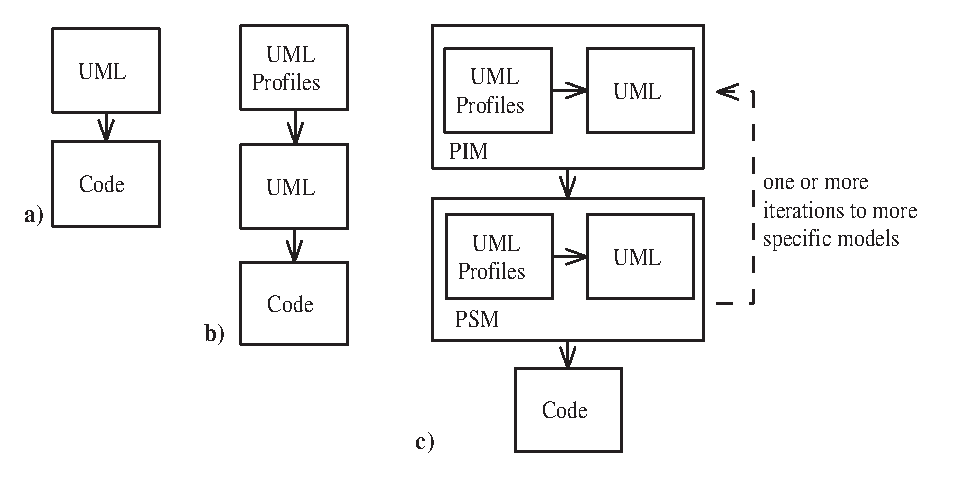
\includegraphics[width=10cm,height=!]{ch02/mda}
	\end{center}
	\caption{MDA Development}
	\label{fig:mda}
\end{figure}

\fig{fig:mda} shows three different ways, how a visual CASE tool can be used to model an application. Although only UML \cite{www.uml} is denoted in the boxes of this diagram, any (meta) model language can be used. The simplest case (a) shows generating code from a visual model which maps directly to the implementation language. Case (a) has been used in the past to generate embedded software. The visual model contains a predefined set of user-defined element classes. Case (a) is usually not very interesting because it supports only an one-to-one mapping into code and hence no automatic injection of the domain concerns is possible.

Case (b) of \fig{fig:mda} uses custom additions to the generic meta-model, in this case through one or more UML profiles, which helps to factor out and to reuse the domain functionality. For example, the UML profile for Enterprise Java Beans (EJB) \cite{www.uml.ejb,www.uml.ejb.omg} \textit{"defines a set of UML extensions that capture the structure and semantics of EJB-based artifacts"} \cite{www.uml.ejb}, mainly by utilizing stereotypes and typed values. The EJB profile captures the semantics of a specific domain, in this case of EJB \cite{ejb21}, in the form of predefined profile entities that can be reused to model applications in this domain. Rather than having to define applications in terms of object-oriented (OO) classes, a designer relying on the EJB profile can directly use EJB concepts, such as, \flqq{}EJBEntityBean\frqq{} or  \flqq{}EJBPrimaryKey\frqq{}. Case (b) represents how most existing CASE tools work.

The third case (c) generalizes case (b) by splitting the transformation of a model to code into several configurable transformation steps to intermediate models. Case (c) stands for the generic MDA scenario, where the created model (known also as \textit{Platform Independent Model} - PIM) is refined into a more specific model (\textit{Platform Specific Model} - PSM), before some executable equivalent is generated. This could require more than one iteration, moving to a more specific model in each iteration, whereby each model uses its own specialized profile. The case (c) implies also that the details of the PSM are automatically inserted into the PIM using appropriate transformations. While case (b) can be used for a product-line, it is the automated model of case (c) that could be of most interest for automated product-lines that require more than one mapping step, in order to postpone some of the design decisions to a latter phase. That is, case (c) supports \textit{progressive refinement} \cite{sf.04} of the application architecture, from a very abstract design model to more specific models, known also as a stratified design \cite{kuhne.03,kuhne.01}. %Case (c) automatically reduces the architectural gap between the product-line abstractions and the implementation of specific applications.

There is no agreement in the MDA community on what is the best way to define PIM to PSM transformations. Often, only the structure of a model is defined graphically in a CASE tool, that is, components, their interfaces and relations. Although it is possible to define method implementations graphically (e.g., by using UML Actions), in practice it is often easier to associate pieces of code directly with the structural model elements, which means that pure visual models are rarely used.

An example of a commercial meta-modeling tool, used to model mobile and embedded software, is MetaEdit+ \cite{MetaEdit.Home} from MetaCase. MetaEdit+ has been used in several Nokia \cite{www.nokia} projects, e.g., graphical user interface modeling for TETRA (TErrestrial Trucked RAdio) devices \cite{MetacaseCase.03}. The main rationale behind MetaEdit+ is that domain-specific visual languages and visual domain-specific abstractions help to automate software development \cite{metaedit.embedded}. MetaEdit+ enables the creation of meta-models for specific domains, and using the elements of these meta-models to model specific domain problems. The domain elements and their relations are presented graphically. Source code artifacts can be associated with parts of interests, and various predefined or customized reports (including source code) can be generated from the models. Model transformations are not supported directly in MetaEdit+, and it basically works based on the model of case (b) of \fig{fig:mda}. 

Another example of a CASE tool is the Generic Modeling Environment (GME) \cite{gme.01}. GME, like MetaEdit+, uses a proprietary meta-meta-model and offers limited support for MOF, as just another meta-model. GME is a university research tool, developed based on the concept of Model Integrated Computing (MIC) and MultiGraph Architecture (MGA) \cite{gme.mic}. While the terminology used in the GME documentation is sometimes peculiar, most of the MGA concepts can be directly mapped to the MOF terminology and MGA could be considered to be a custom case of MOF. % as shown in Table~\ref{tab:GMEMGAVsMOFTerminology}.

Compared to MetaEdit+, GME is limited only on defining meta-models, model constraints\footnote{The UML Object Constrains Language (OCL) is used.}, and graphical models based on these meta-models. Code generation or other reports should be implemented as Visual C++ add-ins, or generated by doing a traversal of the model graph, by using various script languages that can access the GME COM components API. The transformation of the models is supported via graph transformations \cite{gme.graphs} using other tools outside GME. Graph transformations support the case (c) of MDA development of the \fig{fig:mda}. Graph transformations are based on writing transformation (graph rewrite \cite{schurr.graph.94,Blostein-Schuerr02:99}) rules as left-hand and right-hand side subgraphs. The left-hand subgraph, when found in a graph, is replaced with the right-hand subgraph. The specification of rules can be done graphically in a CASE tool, e.g., GME, or by using more formal grammar rules \cite{Rekers-Schuerr02:97}.

Matching of the left-hand side rules in a graph can be simplified by sequencing the order in which the rules are applied \cite{gme.graphs}, or by restricting the form of the left-hand side of a rule \cite{Rekers-Schuerr02:97}. Rule matching can also be simplified by starting on predefined nodes, known as part of the sequence rules for a given domain. Milan \cite{gme.milan} is a framework based on GME, for the simulation of embedded system designs, in particular System-on-Chip (SoC) designs. Apart from GME modeling components, Milan also supports various simulations of the designed systems, using other third-party software. Another GME based system is GRATIS \cite{gme.gratis}. GRATIS supports high-level visual modeling for TinyOS \cite{gme.tinyos}, a small operating system for embedded devices. GRATIS helps to manage the event-based component communication in the TinyOS, reducing the development errors that result from directly maintaining the component interaction files.

Some other approaches, such as, SmallComponents \cite{www.smallcomps}, use predefined UML profiles to generate the entire OS required in an embedded device, by including only those parts that are interesting for an application. Small\-Components-like approaches can be useful for small embedded devices where the entire system is generated at once containing a set of selected predefined applications. A comprehensive list of existing CASE tools can be found in \cite{case.tools}, whereas a list of preferable features for such tools can be found in \cite{uml.tools.criteria}.

Based on the criteria for mobile product-lines listed in \sr{sec:var.mob.pl}, there are several reasons why visual modeling in isolation is not very useful as a variability mechanism.

\begin{itemize}
\item \textit{Partial automation}. Ideally, a visual model can be used to generate code in more than one target language. The final target code is, thus, not very important to a CASE tool. In practice, this requires that the entire functionality is defined visually, which is not preferable in complex application domains, where a lot of specific application functionality must be coded manually. For this reason, CASE tools can easily generate stubs of code for a language, but leave most of the method implementation details to be filled out manually. Various techniques \cite{voelter.generation}, e.g., the template method pattern \cite{dpatterns}, can be used to keep the manually added code separately from the generated code.

\item \textit{Difficult evolution}. Creating product-lines is an iterative process. The domain abstractions are not known from the beginning and they normally evolve as the product-line matures. The final generated code for such abstractions may not be optimal, or completely known from the beginning. Maintaining evolving abstractions visually in a CASE tool could result in additional costs \cite{lop.94}, because the meta-model and all the models based on it must also be maintained.

CASE tools are better suited when the domain abstractions are nearly frozen and well-known. Language abstractions can better support iterative development of product-lines if their implementation and maintenance costs are low. Once the product-line stabilizes, it is usually easy to map domain abstractions, implemented by the programming language(s), to visual modeling elements.

\item \textit{Loss of design information}. Another issue using CASE tools alone, without appropriate support at the language level, is that source code is treated as an end product, similar to the binary code generated by a compiler. Despite comments added by a CASE tool in the generated code it is difficult, or impossible, to preserve the visual model architecture in an easy understandable way. It could be argued that the source code is not important, as long as the model is present. The model hides the details of the code that are not important for a domain. However, given that code must be often edited or completed manually, it is difficult to follow changes and debug it. %Often, CASE tools offer only one way transformations, from model to code, but cannot completely reverse engineer any meaningful design from the code \cite{riel.96}. 
Domain-specific abstractions, when supported directly at the programming language level, help to bridge this architecture gap.

\end{itemize}

\subsection{Domain-Specific Modeling with Language Abstractions}
\label{sec:var.dsa}

This section discusses ways to support domain-specific modeling with language abstractions, rather than with visual abstractions and CASE tools. \textit{Domain-specific abstractions} (DSA) refer to abstractions that are added to, or directly supported by a language, or that are an inherent part of the language, in order to support domain-specific modeling. For example, in the domain of web services special keywords, such as, \texttt{webservice} and \texttt{webmethod}, could be used to denote special treatment of web service constructs by the compiler, e.g., to automatically generate WSDL\footnote{Web Service Description Language. (http://www.w3c.org)} files. Such keywords can be used to define a \texttt{TravelAgent} class, as a web service component, as illustrated in \fig{fig:webservice-dsl}.

\begin{figure}[ht]
\begin{center}
\begin{minipage}{7cm}
\begin{scriptsize}
\begin{lstlisting}[numbers=left,language=Java,frame=leftline]{}
webservice TravelAgent {
  ...
  webmethod GetHotels(){...}
  ...
}
\end{lstlisting}
\end{scriptsize}
\end{minipage}
\end{center}
\caption{A Domain-specific Extension to Implement Web Services}
\label{fig:webservice-dsl}
\end{figure}
 
\noindent There are several benefits from using declarative DSA as a variation mechanism for mobile product-lines:

\begin{itemize}
\item \textit{DSA preserve the architecture of the domain in source code.} Consider the example of the web service abstraction (\fig{fig:webservice-dsl}) as a part of a product-line. When web services are supported declaratively in the language, a single keyword \texttt{webservice} can be used in every place the web service functionality needs to be reused. The source code with the declarative domain abstractions is easier to understand. The code is not considered as the end-product of some generator, which is difficult to modify by hand, but as a means to express the domain design. DSA help to trace the architecture down to code, as well as, to reconstruct the architecture from source code \cite{sf.04}.
%
DSA support automation and reduce accidental complexity\footnote{Complexity related to the particular solution, not inherent in the solved problem itself. The later is known as \textit{essential complexity} \cite{brooks.87}.} in a product-line. While DSA have the same explicit programming model as OO libraries \see{sec:ooframeworks}, they automate the instantiation and usage of the domain abstractions in source code.

\item \textit{DSA can be used as an alternative to visual modeling.} It is easy to support a set of DSA, that are in place for a domain, with CASE tools. For example, an icon in a CASE tool can represent a \texttt{webservice} which will be mapped directly onto the corresponding DSA construct in the source code. Declarative DSA blur the distinction between an explicit modeling step, and directly modeling at the source code level. 
Working directly with the code, to refactor it using DSA, reduces one step in going through a visual modeling tool, but at the same time supports the same level of abstraction. %This can be beneficial, because the proper code abstractions may not be known right from the beginning. 

\item \textit{DSA implementations can be optimized using generative techniques.}  The DSA processing tools have access to the abstract syntax tree (AST), and can directly inject the domain code into the AST locations where the DSA are found. To the end user, the abstractions are still declarative. It is hard to achieve this with object frameworks \cite{dsl-pl.2000, batoryetal.00}, where OO inheritance and composition are exclusively used.

\end{itemize}

\noindent There are several ways to support DSA:

\begin{enumerate}[i.]
\item New languages can be defined from scratch, whose elements directly correspond to abstractions in a particular domain. Such languages are called \textit{Domain-Specific Languages} (DSL) \cite{deursenetal.00}. For example, Maple\footnote{http://www.maplesoft.com/} is a computer algebra system specialized for calculating specific mathematical formulas. Such specialized languages are very effective in some domains. However, often it makes sense to reuse as much of an existing host language as possible when adding DSA.

\item \textit{Embedded Domain-Specific Languages} (EDSL) integrate DSA into a host language \cite{leijen.99,kamin.98}. The host language is often a general-purpose language, e.g., Java, which is augmented with declarative constructs to support one or more domains of interest. An example of an EDSL, is SQLj \cite{www.sqlj}, an embedded SQL engine for Java.

\item Another way to support DSA is indirectly via \textit{general-purpose software abstractions}, which are first added to a host language in order to (a) make it  extensible to support EDSL-like constructs, or (b) to support generic meta-modularization\footnote{These generic modularization mechanisms need to access the meta-model of a language to enable factorizations that are not possible with inheritance and composition alone.} mechanisms not found in the original language. An example of an general-purpose software abstraction for supporting extensibility is the support for \textit{attributes} in .NET \cite{www.dotnet}, or \textit{annotations} added recently to Java. An example of a generic meta-modularization mechanism that can be used to support EDSL is \textit{Aspect-Oriented Programming} \cite{kiczalesetal.97} as supported, e.g., by AspectJ \cite{www.aspectjt,Laddad.aop} \see{ch2:aop}. The general-purpose software abstractions are not specific to any particular domain and can be used to support several EDSL within the same host language.
\end{enumerate}

\noindent In the following, several drawbacks are discussed, which prevent DSA supported by the first two alternatives (DSL and EDSL) from being widely accepted as a variability mechanism for product-lines. Attribute-based DSA are discussed in \sr{c2.sec.dsa.attributes}, while AOP-based DSA are explained in \sr{sec.aop.dsa}.

\begin{itemize}
\item \textit{High start-up costs}. DSA realized with the first two approaches have the highest start-up costs compared to other variability mechanisms, e.g., component libraries, and require careful planning of the expected variability. Adding the DSL start-up costs \cite{hudak98modular}, schematically shown in case (b) of \fig{fig:pl-cost}, such as defining grammar extensions and interpreting declarative
constructs, to the product-line start-up costs devoted to domain engineering \cite{harsu.2001} and variability representation \cite{harsu.2001}, may result in an unacceptable payoff point for a product-line. This motivates the need for technology that reduces the DSL introduction costs in iterative product-lines.

\item \textit{Difficult to evolve.} DSA are also difficult to maintain in order to support product-line evolution. As with every software system, it is very probable that the proper declarative abstractions cannot defined clearly from the beginning. The development is more iterative in the early phases of the product-line. The cost of changing DSA is usually higher than, e.g., that of maintaining libraries or object frameworks. The implementation of the abstractions and their representation needs to be modified, which affects the language grammar and its parsing. The DSA technology should support experimentation during the iterative product-line development.

\item \textit{Accidental costs.} DSA frameworks introduce additional costs not only for implementing the DSA itself, but also for educating the developers to use the abstractions. Last but not least, DSA introduce unnecessary external dependencies of the product-line on third-party frameworks, needed to implement the DSL additions, which may increase the product-line maintenance costs in the long term. There is also a lack of standard parsing tools and DSL supporting API-s in languages, which renders the implementation of reusable DSA difficult. The DSA technology should be part of the programming language supported by the language vendor.

\end{itemize}

%The reason we treat all of these language abstractions in a single group is that the mechanics for implementing them are more or less the same usually resulting is some transformation of the program abstract syntax tree (AST). Program transformation \cite{www.pt, dms.02} can also be used alone without a DSA front-end, in form of program generators.  Several generative techniques exist \cite{generative.00} , where the variability parameters of a solution are used to drive the generation process. Using parameterized code templates\footnote{By template here is meant any parameterized piece of code (by some means), not only C++ templates. Frame based approaches, and other more exotic approaches, such as, framed aspects \cite{framed.aspects} fall also into this category.} and code snippets can shorten up development time of generative solutions. However, generative techniques, when used alone, lack a declarative support for domain abstractions and make it difficult to preserve the domain architecture into the source code. For a compressive overview of such techniques refer to \cite{generative.00}.

\section{Software Containers}
\label{c2sec:containers}

\Kr{ch03} shows how attribute-based DSA can be used as a low-cost DSL alternative to represent domain concerns in source code. Selecting a variability mechanism is not enough to create a product-line. A structured way to organize the domain assets of the product-line is needed. An \textit{architectural abstraction} \cite{harsu.2001} could be combined with one or more variability mechanisms, in order to support product-line creation and evolution. The product-line architecture \cite{harsu.2001} defines and enforces an implementation methodology to represent and to organize the product-line assets \cite{pl.02}. For example, when OO inheritance is used as a variability mechanism, a well-defined hierarchy of the domain assets could be created.

The product-line architecture should define clear extension points for the developers that extend the product-line \see{sec:ooframeworks}. The DSA constructs are connected with the domain assets implemented in the form of OO libraries \see{dsa.connect}. However, when the DSA become easily to implement, there could be a lot of unstructured DSA constructs added to support the product-line. The unstructured DSA interpretation can become a bottleneck for the product-line evolution.  

Several architectural styles \cite{harsu.2001} have been explored for product-lines, e.g., data-flow architectures and virtual machine architectures \cite{harsu.2001}. The interest in this book is (a) in low-cost mechanisms that support the iterative view of mobile product-line development and (b) in automated reuse of product-line assets in specific applications. Following the current trend of component-based development \cite{comp.soft.book}, supported by today's general-purpose OO languages, such as Java and .NET, this book focuses on component architectures \cite{otm,comp.soft.book,comp.soft.book2,assmann.99-comparison} based on \textit{software containers}. Containers place a clear distinction between the domain functionality, organized as low-cost DSA, and the rest of the application specific functionality. %As this section explains, software containers help both with structuring and with the automatic reuse of the product-line assets.

The container abstraction is usually related to server-side enterprise container implementations, e.g., COM+ \cite{comp.services} and EJB \cite{j2ee14}, and could be described by a combination of software patterns \cite{server.patterns.02}. The container abstraction can be used to organize product-line assets for any application domain. A software container serves as a high-level architectural abstraction, used to organize common domain functionality as services and introduce them nearly transparently to an application\footnote{Unlike most real-world containers, a software container offers some kind of support (services) to the object found in (managed by) it.}. This section starts with an overview of two existing enterprise container implementations, COM+ and EJB. The remainder of the section explains how containers can be used in arbitrary domains, and why is it beneficial to use them to organize mobile product-lines.

\subsection{Microsoft COM+}

COM+\footnote{The term COM+ is used here synonymously with Microsoft Transaction Service (MTS).} \cite{comp.services,www.comp} is one of the first wide-spread enterprise containers. It uses an underlying component model based on Microsoft DCOM\footnote{DCOM stands for Distributed COM, whereas COM itself stands for Component Object Model. Both are proprietary component models.} \cite{www.dcom} technology, which allows components to reside nearly transparently in any networked machine. COM+ is mainly intended to facilitate implementation and maintenance of big enterprise applications. Some of the COM+ services, e.g., catalogs, that organize and maintain sets of components, can be used to support any distributed application. A COM+ application can be configured either programmatically, using any (script) language that can access COM objects, or via GUI tools.

A COM+ application consists of two types of DCOM components: (a) \textit{serviced} components that use the services offered by the COM+ container, and (b) \textit{client} objects that interact with the serviced components. Each COM+ component has its own identity and can be manipulated individually if needed. The idea behind COM+ (as with any container) is that application components that use the COM+ services, are developed by leaving out the exact details of service configuration to COM+. The following discussion of COM+ services is based on \cite{comp.services}.

One of the basic services offered by COM+ is a fine-grained security model based on \textit{roles}. Each role has a well defined set of permissions that specify, which components and component resources, e.g., databases, the role is allowed to access. Users are assigned to roles and this determines their permissions.

Transaction management is another service offered by COM+. A transaction is a sequence of operations that is treated as a single logical operation, and enjoys atomicity, consistency (in the terms of invariants), isolation (no side effects), and durability (introduced changes are not lost). The underlying DCOM technology supports distributed transactions relying on a distributed two-phase commit protocol \cite{Coulouris.01}. Users can also define custom atomic resources, using Compensating Resource Manage (CRM) service, to allow any kind of created or acquired resource to take part in a transaction.

COM+ helps to manage the internal state of component instances by distinguishing between \textit{stateless} objects, \textit{cached state} objects, and \textit{persistent} objects. The internal state of stateless objects is not important and does not need to be preserved. The cached state objects can have their state preserved while the application is running in a shared property manager (SPAM)\footnote{Shared Property Application Manager.}, indexed by string keys. The state of persistent objects can be stored in persistent storage directly or in a relational database. 

Object state is related to object life-cycle management. COM+ manages the life-cycle of objects in order to transparently support scalability\footnote{COM+ can also handle load balancing by distributing requests in a cluster of several machines.}. To handle a large number of sporadic clients for an object, COM+ uses Just In Time Activation (JIT). JIT creates an object instance only when it is needed, and passivates it during the idle time to save the system resources. This service is complemented by object pooling, where several instances of a component are kept and reused to re-personify\footnote{This is similar to \textit{virtual instances} in Java EE \cite{server.patterns.02}.} serviced objects every time a specific object is needed by a client. To achieve pooling, a client does not use COM+  objects directly, but via a \textit{moniker}, which is a DCOM abstraction of an instance handle. A moniker can be used to represent any resource. Database connections are also COM objects, so they can be pooled using the same mechanism too.

An important feature for an application is the ability to synchronize its own activities. COM+ deals with synchronization by supporting different threading models known as \textit{apartments}. A component is activated (invoked) always within a specific thread model. The apartment model is specified when the component is deployed in a COM+ application by setting the right apartment type as part of the configuration. Access to multi-threaded apartment (MTA) objects is synchronized by COM+. A related COM+ concept is an \textit{activity}, which represents a set of objects that are used by a single client (similar to a session). Synchronization can also be controlled at the level of the individual activities.

Another related service is Microsoft Messaging Queue (MSMQ), a pu\-blish-sub\-scribe event service often used by COM+ applications. MSMQ can be used alone without COM+, but it is often used for asynchronous message-based object invocations inside COM+. COM+ applications can also use lightweight directory services\footnote{Lightweight Directory Access Protocol (LDAP).} to locate resources and other components via Microsoft Active Directory service.

One of the problems with using COM+ in the past has been its complex programming model \cite{www.comp}. This complexity comes from the fact that DCOM and COM+ add several layers of abstraction, while preserving the underlying details. COM+ \textit{serviced} components are DCOM components, usually written in C++. DCOM introduces an interface declaration language (IDL) and several implicit programming conventions. COM+ adds another layer of explicit and implicit conventions to DOM that must be known and followed to use COM+ successfully. The preservation of all these details of the programming layers made sense back in the early days of COM+ when the technology was not mature. It was useful to be able to experiment with the technology in order to understand the properties of its abstractions and their implementations. Having access to the implementation details enables also manual optimizations for software that has to run in slow machines. Such a detailed programming model with little automation can work only for relatively few and small applications.

In last ten years the situation has quickly improved. As the computer hardware becomes much cheaper than software and there are faster machines, there are also more and larger applications. Language-based abstractions, such as those of .NET \cite{www.dotnet} language families, supported by virtual machines are not considered slow anymore. Long experience with COM+ and DCOM have revealed the repeated coding idioms that could be abstractions on their own. With .NET, \cite{www.dotnet} Microsoft introduced a new, simpler and less restrictive programming model for DCOM \cite{clr.com} and COM+ \cite{com.dnet}, based on meta-data and explicit attributes. The COM+ support in .NET is part of the \texttt{Sy\-stem.Enter\-pri\-seSer\-vi\-ces} namespace \cite{com.dnet}.

\subsection{Java EE and Enterprise Java Beans}
\label{sec.c2.ejb}

Similar to COM+, Java Enterprise Edition (Java EE) \cite{j2ee14} is a container-based technology for enterprise server-side applications. Java EE is based on Enterprise Java Beans (EJB) \cite{ejb21} component model, relying on Java \cite{www.java} component model (beans and remoting)\footnote{These are also proprietary component models.}. Unlike DCOM, the Java component model is simpler to use. Java itself (unlike C++) belongs to the family of languages that maintain meta-data as part of their binaries\footnote{The Java binaries (*.class files) are actually pseudo-binaries that require a virtual machine to be interpreted and cannot be executed directly.}. This simplifies the programming model, e.g., the discovery of the interfaces implemented by a component, is directly supported by the language. Java technology (and Java EE) is an example of the second wave of enterprise containers and technologies used to build them, where more abstraction layers can be afforded as the hardware becomes faster.

While Java EE and COM+ (MTS) offer more or less the same set of services, the terminology is often different. Java EE, for example, uses the term \textit{role} to denote different stages of an application development and life-cycle, e.g., enterprise bean provider, application assembler, deployer, container provider, whereas COM+ does not define any specific terminology for the developer roles. The components are called \textit{beans} in Java EE.

The programming model for the container services is different too. Java EE distinguishes between various types of beans, such as, stateless, session, entity (persistent), and message-driven (event based). Unlike COM+, where the stereotype of a component is specified as part of its configuration attributes, in Java EE components state their type explicitly based on required interfaces specified as part of their implementation and other implicit\footnote{That is, many Java EE component coding rules are not part of the language syntax and cannot be enforced explicitly by the Java compiler.} coding rules, e.g., required method names.

Services offered by Java EE include, for example, security, transaction management, naming, message-based communication and timer service. There are slight differences between these services and the corresponding COM+ services. For example, security in COM+ is not concerned with user authentication, since this is handled by the operating system, whereas Java EE deals with user authentication itself, because it is intended to work in multiple different server operating systems.
Naming (JDNI) in Java EE corresponds to Active Directory services in COM+, whereas message-based communication via message-driven beans is similar to MSMQ. A Java EE bean can use the timer service to register callbacks to be called at a given time or periodically. The timer counters are persistent and callback registration can be treated as a transactional resource (as with CRM in COM+). Object pooling and database connection pooling are also handled by Java EE. Java EE uses the term \textit{virtual instances} \cite{server.patterns.02} for handles to the pooled objects (in COM+ a handle is implemented by a moniker).

The most interesting aspect of Java EE is the evolution of its programming model. EJB, up to version 2.1 \cite{ejb21}, makes use of required interfaces and pseudo-syntactic rules (coding conventions), such as naming rules for method names. Creating a bean implies defining one or more required interfaces. Furthermore, beans that need some form of life-cycle management, must implement required callback methods, e.g., \texttt{ebjActivate()}. Most of these actions are repeated with few variations and could be automatically generated. It is unclear why EJB did not define from the beginning proper abstractions, to deal with such tedious programming tasks, that can be easily automated and made transparent\footnote{When EJB appeared its programming model was significantly easier to use compared to COM+. The .NET programming model for serviced components is now simpler than EJB.}. Third-party tools, e.g., xDoclet \cite{www.xDoclet}, appeared to deal with such inconveniences of the EJB programming model.

EJB is also moving toward a simpler programming model, based on attributes \cite{java.explicit.programming}. The latest EJB specification \cite{ejb30} uses predefined attributes to decorate component implementations, which are now \textit{plain old Java objects} (PoJo-s) with very few implicit coding rules.

\subsection{Using Containers Beyond the Enterprise Domain}
\label{c2.container.domain}

Since the term \textit{container} was made popular by COM+ \cite{comp.services} and EJB \cite{j2ee14}, many people use the term synonymously with enterprise containers. Enterprise containers, such as, COM+ and EJB, are often referred to as \textit{heavyweight containers} \cite{aspectComp.03}, which means:
\begin{enumerate}[a.]
\item COM+ and EJB are container implementations for a hardwired problem domain. The containers are defined exclusively for enterprise server applications, usually involving relational databases as back-ends. These container implementations cannot be reused in other domains.
\item Even for the enterprise domain, COM+ and EJB containers offer only a predefined set of services. EJB and COM+ containers cannot be easily extended to introduce new kinds of services into the domain \cite{aspectComp.03}.
\end{enumerate}

Heavyweight container implementations are tightly coupled with the specific problem they solve. The container as an abstraction is domain independent and open to accommodate new kinds of services. In particular, the container abstraction can be used to conveniently implement automation of application families (product-lines). The functionality offered by a product-line (the reusable assets of the product-line) can be seen as a set of services offered by the product-line container abstraction. The specific application components managed by the container (managed components), known also as \textit{serviced components} \cite{com.dnet}, use the container services as shown in \fig{c2fig:container}. The container service variability parameters are given as part of the deployment specification of an application component in the container. The variability parameters are shown in \fig{c2fig:container} in the form of a deployment interface. The actual implementation may vary depending on the container. The serviced components use the services provided by the container. The connection between the container services and the serviced components is known as \textit{service injection} \cite{com.dnet}.

\begin{figure}[ht]
	\begin{center}
		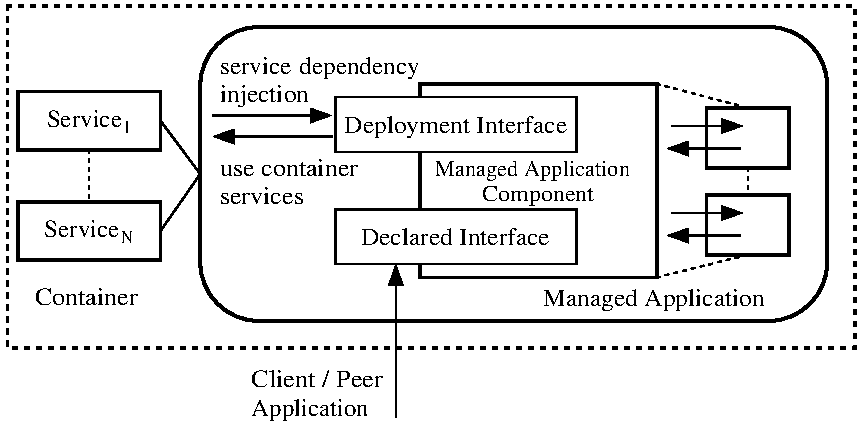
\includegraphics[width=12cm,height=!]{ch02/container}
	\end{center}
	\caption{The Container Abstraction}
	\label{c2fig:container}
\end{figure}

The container abstraction enables a uniform treatment of the services modeling the assets of a specific domain, and the generic services modeling cross-cutting concerns \see{ch2:aop} that may be shared by many applications of different families. The developers of a product-line can manage generic concerns, such as data persistence, within the same container framework as the specific assets identified in a particular domain, e.g., image adaptation required by mobile image processing applications. The container abstraction enables the organization of an \textit{extended} view of a product-line (\fig{c2fig:extended-pl}), whose assets include generic concerns used in the same way, as the assets of a specific application family. An extended product-line is made up of more specific intersecting sub-families that share common assets with each-other, having a network of domains \cite{generative.00}. The shared set of services is represented by the intersection of the different sub-family (assets) eclipses in \fig{c2fig:extended-pl}. The generic concerns are needed by most of the application sub-families within the extended product-line, whereas the application family specific assets are needed only within a family of applications. The uniform treatment of the services enables better share and reuse of the specific services developed for a family, in another family or set of such.

\begin{figure}[ht]
	\begin{center}
		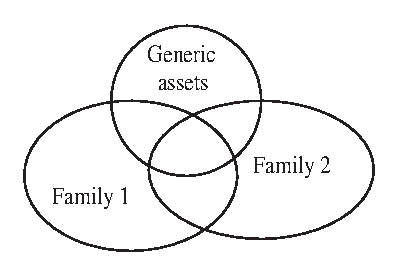
\includegraphics[width=5cm,height=!]{ch02/extended-pl}
	\end{center}
	\caption{The Extended Product-Line}
	\label{c2fig:extended-pl}
\end{figure}


Using the container abstraction to organize a product-line, increases the transparency of reusing the domain services, and results in a better separation of concerns \cite{parnas.72}, because of:
\begin{itemize}
\item \textit{Inversion of control.} The container provides a software indirection for injecting dependencies. The \textit{dependency injection} pattern \cite{fowler.ioc.04}, also known as \textit{inversion of control} (IoC)\footnote{IoC is also expressed as the \texttt{Hollywood Principle}: \textit{"Don't call me, I'll call you."} \cite{spring.article.03}. See \cite{fowler.ioc.04} for a discussion as why the term \textit{dependency injection} is preferable to IoC.}, implies that a component does not explicitly obtain the services it needs but rather, declares its dependency on them by following certain conventions. The declared services are then provided transparently to the component, as necessary, by the environment \cite{lorenz.96,ea.05}. Dependency injection \textit{"moves the responsibility for making things happen into the framework, and away from application code"} \cite{spring.article.03}.

The container connects the product-line services and the application-serviced components in a transparent way. When a service component library is used directly, the exact interface of the service components should be known to the application and be referenced explicitly \see{c2sec:implement}. This is problematic, not only when the interface of the library changes, but also when the library is maintained and several versions of it appear. When inheritance is used, e.g., in a framework, the fragile base-class problem can be encountered \cite{Mezini.97,comp.soft.book,Nathanael.04}, as the base classes evolve. The container abstraction separates the need for a service, from the need to explicitly reference the implementation of the service. The exact service references are introduced transparently to the managed application component.

\item \textit{Improvement of modularization.} The concerns addressed by a product-line are often of a cross-cutting nature. They involve functionality that is needed in more than one place in an application, and negatively affect the overall modularization \cite{Crosscutting1.03,Crosscutting2.03}. The transparent dependency injection, offered by the container, allows developers to focus on those concerns that are specific to application components. The cross-cutting service concerns of the product-line are then introduced automatically by the container. %With a container it is easy to keep the concerns separated in any point in the future, because application components implementation is stored before it is deployed in the container, not after it.

\item \textit{Automation of the development process.} The container abstraction automates the development of applications in a product-line. Product-line automation significantly decreases the development and maintenance costs. The maintenance is improved because the container offers a centralized point to isolate specific middleware services from an application. The container abstraction offers a structured and centralized \textit{object transaction monitor} (OTM) \cite{otm}. This makes it easier to maintain and port mobile application families when the underlying middleware changes.

\item \textit{Implementation architecture.} The container abstraction is a high-level architectural abstraction. It does not replace the usual techniques for product-line implementation, e.g., libraries and code generation. It rather serves as an umbrella for all possible technologies that can be used. One or more technologies can be combined together, to implement the container abstraction in a way that is convenient for a certain domain. %The container places a clear structure on the ways these technologies are used to introduce well-known domain services into a specific application.

\item \textit{Separation of developer roles.} As stated in the Java EE specification \cite{j2ee14}, the container abstraction helps to divide developers in clear distinguishable categories, according to the application development roles: (i) developers that implement the container functionality; (ii)  developers that implement services for the container; (iii)  developers that implement managed applications using the container; (iv) developers that deploy the managed applications into the context of a container. These roles are clearly distinguishable and could be used to properly structure all developers that work with a product-line in an organization.

\end{itemize}

\noindent The container automation has also a few drawbacks depending on the implementation:
\begin{itemize}
\item \textit{The need to learn new coding conventions.} Explicit or implicit coding conventions must be followed by a component implementation if it is going to be used inside a container. These conventions should be learned and properly used by the programmers. For example, an object of a managed virtual instance \cite{server.patterns.02} must not contain methods that return the \texttt{this} pointer directly. This coding convention is required, because otherwise a client would always obtain a different physical reference to the same logical object.

\item \textit{No specialized language support for the coding conventions.} Cheeking implicit coding conventions automatically may be difficult. Explicit coding conventions can be automatically checked, but must be introduced and learned. Explicit coding conventions could be in the form of required interfaces, e.g., \textit{EJBMessageBean} in EJB \cite{ejb21}, or based on some form of DSA, e.g., using additional keywords. Implicit coding conventions are harder to check automatically than the explicit coding conventions are, but require no special syntax to be supported.

\item \textit{Traceability problems because of indirection.} Another related problem is testing and debugging. The indirection introduced by the container makes it difficult to understand the overall functionality of a managed component. This makes it more difficult to debug and test the implementation of the managed components. Nevertheless, debugging can be supported with proper tools and built-in container support for traceability \see{sec.tango.trace}.
\end{itemize}

\subsection{Mobile Containers}
\label{c2.mobile.container}

This book introduces the use of containers to organize mobile software product-lines for J2ME MIDP \cite{www.j2me,www.midp} \seec{ch05}. The container abstraction needs to be specialized in order to reflect the characteristics of the MIDP \cite{www.midp} domain. The mobile software is usually a combination of server-side software and client-side software on the mobile device. Because of limited capabilities of mobile devices, it is desirable to execute as much of the application functionality as possible on the server-side. Ideally, mobile applications should be thin clients. This is not possible for most mobile applications, because a mobile device usually has only sporadic network connectivity. The mobile applications should be able to function even when no network connectivity is available, or to keep at minimum the on-line time, to reduce the connection costs.

Support on the server-side is also needed for mobile applications. For example, images need to be resized to adjust their resolution (or HTML pages need to be converted to WAP \cite{www.wap} format, in a WAP-portal), before they are sent to a mobile device. The data need to be prepared on the server-side, before are sent to a mobile device. Data adaptation can be done transparently from the rest of server-side applications, by using some form of the adaptive-proxy pattern \cite{fox96adapting}, before the data are sent to a mobile device application.

To address mobile software product-line issues, this book introduces the notation of a \textit{mobile container}, which is a special kind of container for managing mobile client applications \seec{ch05}. A mobile container helps to organize services needed by a mobile client application and can be used to support product-lines for mobile applications. The implementation of the offered services is split into a server-side part, and a client-side part running on the mobile device. The client-side implementation must be optimized to reduce the number of abstraction layers resulting from the container indirection. For a managed application running on the mobile device, the container services are transparent. It is the container's responsibility to coordinate the client and the server parts and to provide the requested services to the client applications.

\Kr{ch05} elaborates more on how mobile containers can be structured and about the technology that can be used to build open \textit{container families}, which can be customized to support product-lines for more than one domain. The container implementation introduced in \kr{ch05} is based on a generic Java-based framework, and is open for adding new services for arbitrary domains. The implementation is then specialized with a set of service plug-ins for J2ME MIDP \cite{www.j2me} applications.

\section{Container Implementation Techniques}
\label{c2sec:implement}

%The container abstraction can be implemented using any of the variation mechanisms described in this chapter, e.g., visual CASE tools (UML profiles), or DSA. As noted in sections~\ref{sec:var.mob.pl} and~\ref{sec:var.dsa}, declarative language support for architectural abstractions, such as containers, helps to preserve the design of an application in its source code. However, introducing and maintaining DSA abstractions is often costly. For this reason, container developers have explored various techniques. Some of these techniques try to employ existing language abstractions, whereas others go more in the DSA direction.

The ultimate goal of a container is to provide services transparently to its managed components. Ideally, the components are developed in isolation from the environment \cite{lorenz.96,ea.05} where they are used. The component implementation does not need to know anything about a specific container environment. The component, nevertheless, needs to specify what kind of services (other components) it expects from the environment.


\begin{figure}[ht]
	\begin{center}
		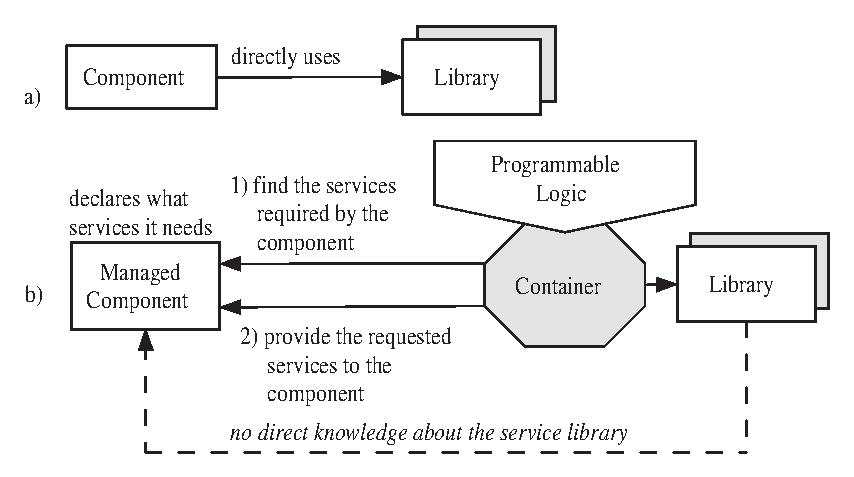
\includegraphics[width=10cm,height=!]{ch02/ioc}
	\end{center}
	\caption{Container Service Dependency Injection}
	\label{fig:con-inject}
\end{figure}

The lightweight coupling of a component with the container environment can be achieved using additional levels of abstraction. Instead of providing a component with direct access to the needed services, as in case (a) of \fig{fig:con-inject}, an agreed convention based on some form of \textit{inversion of control} \cite{fowler.ioc.04} abstraction can be used, as shown in the case (b) of \fig{fig:con-inject}. In case (b), the managed component only declares the services it needs, e.g., by using DSA constructs. The managed component does not have a direct knowledge of any particular service implementation. The container contains the functionality to provide the requested services to the component. The container implementation could provide only a predefined set of services, or the container can have programmable logic to be extended to provide arbitrary services \seec{ch05}.

The most interesting point in a container implementation is, thus, how to define abstractions for \textit{programmable dependency injection}, i.e., how to define dependencies of a managed component programmatically after the component has been created. Based on the terminology defined in \cite{java.compost}, this section distinguishes between \textit{invasive} and \textit{non-invasive} container implementation techniques and gives some examples for each case. Each of the discussed implementation techniques can be seen as a fine-grained variation mechanism.

\subsection{Non-Invasive Container Implementation Techniques}

Non-invasive container implementation techniques are based on pure object-oriented (OO) mechanisms mainly, interfaces, composition, inheritance and reflection. They do not need any special language support, and can be easily implemented in any existing OO language\footnote{Techniques for non OO languages also exist, but these languages will not be considered.}. In a non-invasive technique, there are no components / units more privileged than the others with respect to their power to access and modify other components / units. The entire component access goes through the declared (public) interfaces and uses only standard OO techniques, i.e., non-invasive techniques respect the OO encapsulation.

There are three main ways to inject component dependencies using non-invasive composition techniques: \textit{constructor injection}, \textit{setter injection}, and \textit{interface injection} \cite{fowler.ioc.04}. Almost all implementations of these techniques require reflective introspection support, i.e., internally they use some form of a reflection API. The discussion of non-invasive techniques in this section is based on \cite{fowler.ioc.04}. To demonstrate the \textit{constructor injection} and the other techniques, an example of a Java MIDP based game score class \cite{www.j2me} will be used, shown in \fig{c2f:gamescore1}. The example is made of a \texttt{Ga\-me\-Sco\-re} class, whose internal state needs to be saved in the local memory of a mobile device.

\begin{figure}[ht]
	\centering
	\begin{minipage}[b]{8.5cm}
	\begin{center}	
\begin{scriptsize}
		\begin{lstlisting}[numbers=left,language=Java,frame=leftline]{}
interface Serializer {
   public void Save(string id, byte[] data);
   public byte[] Load(id);
}

class RawSerializer() implements Serializer { ... }

class GameScore() {
   public GameScore(Serializer sr) {	...	}
	
   public void Save() {
      sr.Save(this.GetId(), this.GetData());
      ... 
   }
   ...
}	
		\end{lstlisting}
		\end{scriptsize}
	\end{center}
	\caption{GameScore Serialization Example}
	\label{c2f:gamescore1}
\end{minipage}	
\end{figure}

The \texttt{Se\-ria\-li\-zer} interface (lines 1 - 4) in \fig{c2f:gamescore1} declares operations for saving any data in the device memory, that can be represented as byte arrays. The \texttt{Raw\-Se\-ria\-li\-zer} class, in line 6, implements the actual serializing functionality. To keep things simple, it is assumed that the \texttt{Ga\-me\-Sco\-re} class contains two methods \texttt{Get\-Id()} and \texttt{Get\-Da\-ta()}, which return a string ID for the object (the key), respectively its data as a byte array (the value). An automatic implementation of the \texttt{Get\-Da\-ta()} method will be shown in \sr{ch2:inv}.

\begin{figure}[ht]
	\centering
	\begin{minipage}[b]{8.5cm}
	\begin{center}	
\begin{scriptsize}
\begin{lstlisting}[numbers=left,language=Java,frame=leftline]{}
class GameScore() {
   private Serializer sr = new RawSerializer();
   
   public GameScore() {	...	}
	
   public void Save() {
      sr.Save(this.GetId(), this.GetData());
      ... 
   }
   ...
}	
		\end{lstlisting}
		\end{scriptsize}
	\end{center}
	\caption{Direct Dependency Access}
	\label{c2f:direct}
	\end{minipage}	
\end{figure}

To demonstrate the constructor injection, the \texttt{Ga\-me\-Sco\-re} constructor expects an object implementing the \texttt{Se\-ria\-li\-zer} interface. The \texttt{Ga\-me\-Sco\-re} class can be connected directly to \texttt{RawSerializer}, as shown in \fig{c2f:direct}, which is equivalent in functionality and simpler to implement. This method would tie the \texttt{Ga\-me\-Sco\-re} implementation to the \texttt{Raw\-Se\-ria\-li\-zer} class. The connection between \texttt{Ga\-me\-Sco\-re} and \texttt{Raw\-Se\-ria\-li\-zer} is explicitly coded. The programmer decides about the exact implementation of serialization to use, at the time the \texttt{Ga\-me\-Sco\-re} class is coded. Thus, the direct connection is the least flexible dependency method.

\begin{figure}[ht]
	\centering
	\begin{minipage}[b]{12cm}
	\begin{center}	
\begin{scriptsize}
\begin{lstlisting}[numbers=left,language=Java,frame=leftline]{}
MutablePicoContainer pico = new DefaultPicoContainer();
pico.registerComponentImplementation(RawSerializer.class);
pico.registerComponentImplementation(GameScore.class);
GameScore gameScore = (GameScore) pico.getComponentInstance(GameScore.class);
gameScore.Save();
		\end{lstlisting}
		\end{scriptsize}
	\end{center}
	\end{minipage}
	\caption{Constructor Dependency Injection with PicoContainer}
	\label{c2f:pico1}
\end{figure}

%for all
\begin{dinglist}{43}

\item \textit{Constructor injection}. \fig{c2f:pico1} shows how the \texttt{Ga\-me\-Sco\-re} class of \fig{c2f:gamescore1} and the \texttt{Raw\-Se\-ria\-li\-zer} instances could be coupled programmatically using PicoContainer \cite{java.picocont}. PicoContainer assumes that the classes to be connected already define constructors for the appropriate service parameters. 
The \texttt{pico} container object contains all dependency information required to connect the \texttt{Ga\-me\-Sco\-re} and \texttt{Raw\-Se\-ria\-li\-zer} instances. To connect \texttt{Ga\-meSco\-re} with a new \texttt{Se\-ria\-li\-zer}, for example \texttt{Remo\-teSeria\-li\-zer} that can save data to a server when there is a network connection present, only the \texttt{Raw\-Se\-ria\-li\-zer.class} need to be replaced with the new \texttt{Remo\-te\-Se\-ria\-lizer\-.class} in the container. The PicoContainer indirection assures that \texttt{Ga\-me\-Sco\-re} will never know directly about a particular \texttt{Se\-ria\-li\-zer} implementation it is using. Having a \texttt{Se\-ria\-li\-zer} interface is not a requirement for PicoContainer. It can also connect instances of classes directly by examining their interfaces and finding the appropriate services based on the method signatures by using reflection. 

\item \textit{Setter injection} is similar to constructor injection, but makes use of the assumption that component classes implement appropriate setter methods for service components they depend on. In the example of \fig{c2f:gamescore1}, this could be accomplished by having the \texttt{Ga\-me\-Sco\-re} class define a \texttt{setSe\-riali\-zer(Se\-ria\-li\-zer sr)} method. A container implementation that relays mainly on setter injection is Spring Java / Java EE Application Framework \cite{www.spring}. There are several semantic differences between setter and constructor injection approaches. The setter injection provides more flexibility:
\begin{itemize}
\item An object can be created even though not all dependency objects it requires are available. This is not possible with the constructor injection, where all dependencies must be known when the object is created.
\item When using the setter methods, dependencies can be changed during the lifetime of an object. Often, a certain service needs to be attached to different existing instances and this is not possible with constructor injection. This can be useful, for example, when a virtual instance \cite{server.patterns.02} in an EJB container needs to be connected with a previously saved object state. With constructor injection, a new object must be always created, whereas with setter injection existing objects can be reused.
\end{itemize}
There are also some drawbacks that result from the flexibility of the setter injection:
\begin{itemize}
\item Given an existing component instance, it cannot be guaranteed that the instance is fully and properly initialized in the context of a container, or whether it needs more dependencies to be injected. Repetitive checks need to be performed every time an object instance is used to make sure that the dependencies are properly configured.

\item An explicit search must be carried out by the container to find the appropriate setter methods and decide for the right service objects to be passed, based on the setter method signature. This requires scanning the component interface for all possible methods, finding whether there are any setter methods, and matching the signatures of setter methods to the service components. Hence, the setter injection takes in average longer than the constructor injection. In the later, only the constructors need to be checked when new instances are created.
\end{itemize}

The setter injection is an example of what will be called a \textit{pseudo-syntax} convention to add custom semantics to a language \see{ch03.pseudo.syn} without changing its grammar. A pseudo-syntax construct is not an explicit part of the grammar syntax of the language. It is a \textit{coding convention} and is not checked by the compiler. In this case, the \textit{set} prefix is used as an implicit \textit{syntactic pattern} to define the setter injection. 

\item \textit{Interface injection} is a generalization of the setter injection. Instead of having required constructors or setter methods in the game score example, an interface \texttt{In\-ject\-Se\-ria\-li\-zer} with a single method \texttt{in\-jectSe\-ria\-li\-zer(Se\-ria\-li\-zer sr)} is defined, and the \texttt{Ga\-me\-Sco\-re} class will implement it. Based on the \texttt{In\-jectSe\-ria\-li\-zer} interface, an interface injection container implementation can couple the object and the service\footnote{The reader is referred to \cite{fowler.ioc.04} for an example of a framework that uses interface injection.}.

The interface injection pattern has the same benefits and drawbacks as the setter injection.
However, interface injection improves the search by making the injection points explicit. The container needs to search only for the implemented interfaces and their methods to find what services need to be provided to a given component. No pseudo-syntax checks are required, such as, the check for the \textit{"set"} method prefix. Adherence to pseudo-syntax constructs cannot be checked at the compile-time. Hence, employing pseudo-syntax constructs as a mean of interfacing with the dependency container is more error prone that using interfaces for the same purpose. Pseudo-syntax checks rely also extensively on string pattern matching, which is a resource consuming task when done repeatedly at run-time.

When interfaces are used to denote custom semantics by tagging class implementations, they are known as \textit{marking interfaces} \cite{design.attrib}. The interfaces that require trivial method implementations just for the sake of service injection will be treated as marking interfaces here. In an invasive container \see{ch2:inv}, a marking interface does not need to contain methods that must be implemented in the classes that use the interface. An invasive container can modify a component decorated with \texttt{In\-ject\-Se\-ria\-li\-zer} interface to properly inject the required serialization service. In non-invasive containers marking interfaces may contain methods. 

Marking interfaces can be used to add semantics to components in languages that do not provide explicit attributes, such as, Java 1.4 \cite{www.java,java.attrib4j}. They can be used to declare dependencies, as in the case of injection pattern, or other properties that a component must have\footnote{A well-known example is the use of the \textit{Se\-ria\-li\-zable} interface in Java. Another example is the \textit{Null Object} pattern \cite{refactor.99}, where a class defines specific functionality for the null case by using inheritance from a Null (marking) interface.}. Marking interfaces have also some problems. As \kr{ch03} discusses, the number of marking interfaces can grow exponential in a system, in the case when interfaces are used to support component variability.

\end{dinglist}

There are also several other non-invasive techniques, less flexible than the ones explained above. They are used less frequently to implement the dependency indirection in a container. Only \textit{service locator} \cite{fowler.ioc.04,j2ee.without.ejb.04} and \textit{mix-ins} \cite{bracha90mixinbased,Ernst.99,flatt98classes,Duggan.00} will be briefly considered in this section.

\begin{dinglist}{43}

\item \textit{Service locator} makes service acquisition explicit. The idea is to locate the services of interest explicitly by consulting a (well-known) object registry. The registry location could be hardwired in the component implementation, or it can be indirectly passed to it using any of the above dependency injection techniques. In the service locator case, the  \texttt{Ga\-me\-Sco\-re} example would contain code to get the serializer object directly from the object registry as in \fig{c2f:locator}. Any directory (LDAP\footnote{Lightweight Directory Access Protocol.}), trading, or naming service can be used as a locator repository for objects. The locator must find the required service object and properly initialize it. The requested registry object path (e.g., a relative path \textit{"Lo\-cal\-Se\-ria\-li\-zer"}, or an absolute path \textit{"jndi://mobcon/services/LocalSerializer"}) can be hard coded in the application, or read from a configuration file.

\begin{figure}[ht]
	\centering
	\begin{minipage}[b]{12cm}
	\begin{center}	
\begin{scriptsize}
\begin{lstlisting}[numbers=left,language=Java,frame=leftline]{}
ServiceLocator locator = ...
LocalSerializer s = (LocalSerializer)locator.loadService("LocalSerializer");
		\end{lstlisting}
		\end{scriptsize}
	\end{center}
	\caption{Constructor Dependency Injection with a Service Locator}
	\label{c2f:locator}
	\end{minipage}	
\end{figure}

The service locator offers less automation than the other techniques presented above. Finding services is explicitly encoded, and the kind of service the programmer is asking for, must be exactly know \cite{j2ee.without.ejb.04}. Furthermore, service locator adds accidental complexity to the component's implementation. The service locator is sometimes used as a complementary technique to other dependency injection mechanisms in a system. For example, JNDI \cite{www.jndi} is used in Java EE to access secondary application resources, e.g., images and Java Server Pages (JSP).

\item \textit{Inheritance and Mix-ins} can also be used to emulate indirect dependencies \cite{dip}. Mix-ins \cite{bracha90mixinbased,Ernst.99,flatt98classes,Duggan.00} factor out properties that cross-cut more than one class \cite{riel.96}. In the particular case of the containers, a mix-in can contain the context for a container service. Mix-ins can be implemented using multiple-inheritance, or with templates in the languages that support them \cite{SmaragdakisBatory.02,generative.00}, e.g., with C++ templates, or Java generics.

The inheritance based techniques are usually static\footnote{There are also exceptions, e.g., Rondo \cite{rondo.97}.}, i.e., static linking (deployment) of components is required. For this reason, inheritance composition techniques are usually less flexible than other non-invasive techniques. No known container implementation exists that relies exclusively on inheritance techniques. The mix-ins technique appears often in different forms in different systems \cite{genvoca.94}, which is why it was discussed as an separate alternative here.

\end{dinglist}

\subsection{Invasive Implementation Techniques}
\label{ch2:inv}

%Invasive techniques access the implementation of a component directly, usually relying on the Abstract Syntax Tree (AST) of a program, ignoring the declared (public) interface of the component or making use of the knowledge about the components internal implementation details.

If a container is considered to be a strict component system in the OO sense, then only the non-invasive techniques make sense. They respect the integrity of individual components and operate in accordance with the OO encapsulation rules. A container in this case contains non-invasive code to connect the application components with the container predefined services (other well-known components). The container services are just other components. A well-designed container (non-invasive, or invasive) is usually extensible, i.e., new service components may be added.

Another view of a container is as a transformation system\footnote{The term \textit{transformation} is used here to include any generation or transformation technique that requires some form of AST, or equivalent program structure, processing. Sometimes, the same technique can be supported with generative techniques, or with run-time support. No distinction will be made between the two techniques. The run-time support will be considered to be a specialized optimization.}, much like a compiler / transformer. In this case, the components used inside the container environment need to be somehow transformed, so that the expected dependencies are injected into their inner implementation. The container in this case is a programmable transformer, whose input consists of the components, container services (other well known components), and a specification how to connect the first two with each-other. The specification can be given explicitly in some particular syntax, or it can be implicitly inferred from the implementation of components. The details of the specification are used to create \textit{the glue code} \cite{halloway.02} that connects the components with services. The output of such a transformation is a system, where the components and the services are properly connected with each-other by conventional OO mechanisms.

\textit{Invasive techniques} support the transformation view of a container. Invasive techniques require either special language features\footnote{Such as, the ability to access and (arbitrarily) manipulate the source AST, or the run-time meta-model of the program.}, or external frameworks that provide means to mutate the internals of a component, surpassing the usual OO techniques. Invasive source code or binary mutations may not be directly supported by the target language, in which the original component is written. Invasive techniques do not respect the OO encapsulation and depending on the implementation, they can change a component arbitrarily.

An invasive technique can introduce changes to the component internals, or just read the component internals to introduce non-invasive changes \see{attrib.trans}. That is, the invasive techniques can be \textit{read-only} or \textit{read / write}. Read-only invasive techniques can be treated as non-invasive. However, the read-only invasive techniques will be classified as invasive here, because they require access to component internals which are not visible through the declared interface of the component. An example is the use of the Reflection API in Java. By default, the Reflection API  returns only the public members of a class, and is non-invasive by the definition. The private methods can be accessed by changing member access permission by using the \texttt{Reflect\-Permi\-ssion} class. This latter case will be treated as a form of the read-only invasive access to a class.

A distinction is made in \cite{java.compost} between invasive techniques that use \textit{explicit} and \textit{implicit} \textit{hooks}. A \textit{hook} is defined as an accessible point of the component interface or implementation that can be used to modify the component and to inject code into it. Explicit or declared hooks are hooks that are defined explicitly by the programmer to indicate that the code associated to them will change. An example would be the decoration of a method with an attribute, or a special predefined prefix in its name. Implicit hooks can be any accessible point of a component, even those that are not foreseen by the original developer, e.g., a method call at run-time.

Accessible points of a component depend on the technology used to access the description of the component's implementation. Not all technologies are equally expressive. For example, method internals cannot be accessed using OO reflection alone. Therefore, the code inside a method cannot serve as a hook when the reflection technology is used. The term \textit{hook} will not be used here anymore, because it is also used to name some special callbacks in event-driven applications. The term \textit{hook} in \cite{java.compost} is more or less used with the same meaning as the term \textit{joinpoint} in Aspect-Oriented Programming \cite{kiczalesetal.97}, which is more specific and will be used in this chapter. Joinpoints will be further discussed in \sr{ch2:aop}.

Any system that supports some form of access and manipulation of the abstract syntax tree (AST), e.g., JTS \cite{batory98jts}, can be used to implement invasive containers. Invasive techniques will be illustrated here by an example which uses syntax similar to COMPOST~\cite{java.compost}.

\begin{dinglist}{43}

\item \textit{Invasive Example.} The service dependency injection in the \texttt{Ga\-me\-Sco\-re} example of \fig{c2f:gamescore1} could be easily implemented with invasive techniques. The AST of the \texttt{Ga\-me\-Sco\-re} class needs to be traversed to add / modify the serialization service variable and make it point to the requested service. Given that this case is trivial, the example will rather show how the \texttt{Get\-Da\-ta()} method of the \texttt{Ga\-me\-Sco\-re} class could be implemented with invasive techniques. This method returns a byte representation of a \texttt{Ga\-me\-Sco\-re} object's state. 

The example of the \texttt{Get\-Da\-ta()} method implementation is more interesting, because it shows how the invasive techniques can be used to introduce functionality inside a method. This is impossible to realize directly with non-invasive techniques. Part\footnote{To keep the discussion simple, it is assumed that the \texttt{Ga\-me\-Sco\-re} class includes only simple primitive types. Object serialization should follow the containment dependencies to properly serialize all field objects. Checking of the special cases is also omitted from the code.} of the implementation of the \texttt{Get\-Da\-ta()} method is illustrated in \fig{c2f:getdata}, by using pseudo-syntax similar to the one found in COMPOST \cite{java.compost}.

\begin{figure}[ht]
	\centering
	\begin{minipage}[b]{12cm}
	\begin{center}	
\begin{scriptsize}
\begin{lstlisting}[numbers=left,language=Java,frame=leftline]{}
CompilationUnitBox box = 
    compositionSystem.createCompilationUnitBox("GameScore.java");
List<FieldBox> fields = box.findField("*");
//<<check if there are fields>>
MemodBox method = compositionSystem.createMethodBox("GetData");
//<<specify method parameters, scope and return type>>
//<<add code to the method to init an in-memory binary writer>>
for(FieldBox field : fields)
{
    method.addString("binaryWriter.Write(" + field.Name + ");\n");
}
//<<add code to method to properly return bytes from binaryWriter>>
box.addMethodBox(method);
		\end{lstlisting}
		\end{scriptsize}
	\end{center}
	\caption{The Invasive Implementation of the \texttt{GetData()} Method}
	\label{c2f:getdata}
	\end{minipage}	
\end{figure}

All the member fields of \texttt{Ga\-me\-Sco\-re} class are accessed, and based on them the code for a new private method \texttt{Get\-Da\-ta()} is generated. \texttt{Get\-Data()} serializes the data of each field in a memory binary stream. The example of the \fig{c2f:getdata} accesses first the Java class (GameScore.java) and implicitly parses it in lines 1 - 2. Then, it builds a list of all fields found in the input class (line 3). It creates a new method node (line 4) for the \texttt{Get\-Da\-ta()} method that needs to be added. The details of the method node, such as its return type and the parameters, are specified in lines 6 - 7 (not shown). The example traverses over all the fields which are found in the fields list. For each field, code to serialize its contents into a series of bytes is added to the new \texttt{Get\-Data()} method (lines 8 - 11). Finally the created method is added to the class (line 13)\footnote{The code which saves back the class after its modification is omitted.}. 

A similar method \texttt{Set\-Da\-ta(by\-te[]\- data)} that reverses the serialization process could also be generated at the same time.

\end{dinglist}

While a Java source code unit (*.java) is shown in this example, the input could also be a compiled Java class (.*class). The class file (bytecodes) can be processed either at load-time or at run-time if the particular invasive system has the support for that.

As illustrated by this example, even for relatively small tasks, invasive compositions require tedious coding. This is an inherent property of API-based generation systems \cite{voelter.generation} due to the programming indirection. Rather than writing the source code directly, code that generates the code is written. The indirect code has also to deal with each special case.
%
Code templates and textual pieces of code can be used to shorten the amount of code that needs to be written programmatically and debugged indirectly. The \texttt{Get\-Da\-ta()} method could also be created from a predefined source code template. The template would then be bounded \cite{java.compost}\footnote{That is, template parameters will be replaced by the specific code for the use-case.} to the specific code generated to serialize each field. Suitable predicates, which are used to control the AST node selection and iteration, as those in \cite{trans.strategy.01}, can also reduce the needed work.


\subsection{Non-Invasive versus Invasive Techniques}

Most software composition problems, such as the dependency injection, can be solved either with non-invasive or invasive techniques. However, there are several differences between the non-invasive and invasive techniques with regard to:

\begin{itemize}
\item \textit{Automation} - invasive techniques help to achieve more automation, because they can be customized for the problem at hand. Invasive techniques reduce better the accidental complexity of the solution.
\item \textit{Flexibility} - invasive techniques are more flexible for making changes inside components. Invasive changes are either not possible with non-invasive techniques, or require many explicit indirection layers to be implemented. 
\item \textit{Dynamicity} - non-invasive techniques enable changing the binding of the components with services at the run-time. Invasive techniques are static: they usually operate over the AST of a program. Invasive techniques could also be implemented dynamically when appropriate run-time support is provided.  %streamloom example
\item \textit{Ease of the implementation} - non-invasive techniques require only OO mechanisms which are found by default in many languages. Invasive techniques require meta-language extensions or external frameworks that need to be maintained explicitly as the core language changes.
\end{itemize}

Depending on the particular properties of the specific systems, sometimes dynamicity is preferred to flexibility and automation, and sometimes using existing language support is preferred to using external frameworks. For mobile containers, the declarative language constructs are supported with attributes, so that the static invasive techniques make more sense. Maximum automation is needed and the generic dynamicity of non-invasive compositions is not required in the addressed MIDP \cite{www.midp-ota} systems \seec{ch05}. \Sr{sec:var.mob.pl} listed several preferable properties of the variability mechanisms for mobile product-lines. Table~\ref{tab:InvasiveVSNonInvasive} summarizes how these criteria are supported by invasive and non-invasive techniques, in the context of attribute enabled mobile product-lines.

\begin{table}[ht]
	\begin{center}
		\begin{tabular}[t]{|l||l|l|}
\rowcolor[gray]{.7}
\hline
Criteria & Invasive & Non-Invasive \\
\hline
Explicit programming model, possibly DSL based & + & - \\
Enable automation & + & - \\
Low start-up / evolution costs & - & + \\
Domain-specific optimizations & + & - \\
\hline
		\end{tabular}
	\end{center}

	\caption{Techniques for Attribute Mobile Containers - Invasive versus Non-Invasive}
	\label{tab:InvasiveVSNonInvasive}
\end{table}

As shown in Table~\ref{tab:InvasiveVSNonInvasive}, invasive techniques can be used to support an explicit programming model with DSA at the language level. The focus is in the invasive interpretation of explicit joinpoints modeled with attributes. Invasive techniques can be used to automate attribute-based DSA transformation and also to process implicit joinpoints \see{ch2:aop}. Explicit attributes, combined with invasive techniques, help to reduce the accidental complexity of the programming model. The last line of Table~\ref{tab:InvasiveVSNonInvasive} shows that, for mobile containers, invasive techniques also support better the optimizations, e.g., specific selection of service code, or reduction of the abstractions being used.

The only benefit of non-invasive techniques with regard to the criteria in Table~\ref{tab:InvasiveVSNonInvasive} is that they do not require any special language support and have lower start-up costs. That is, non-invasive containers are easier to implement.
However, non-invasive techniques do not support an explicit declarative programming model. This means that more lines of code need to be written with non-invasive techniques. Therefore, non-invasive techniques offer less automation than invasive ones. Appropriate lightweight attribute-based DSA technology can help to reduce the startup costs of invasive DSA techniques and to preserve the DSA automation benefits.

Invasive techniques have several liabilities that need to be addressed:

\begin{itemize}
\item \textit{Lack of language technology support.} Invasive techniques may not be directly supported by the language. Source-to-source transformers require access to the AST of the component code. For languages that support binary meta-data, such as Java \cite{www.java}, transformations at binary level can be used. Some equivalent of source code AST is preserved and need to be accessed and manipulated.  Not all OO languages offer such AST access as part of their libraries. Third-party parser tools need to be used. These tools should be explicitly maintained when the target language changes. Third-party meta-programming frameworks increase the overall cost of the container implementation\footnote{For example, third-party tools used to parse Java code or manipulate Java binaries have difficulties moving from JDK 1.4 to JDK 1.5. JDK 1.5, introduced a lot of new syntax and the binary meta-data were slightly enriched. The Java vendor (Sun) does not support any transformation interface for Java binaries.}, and could result in higher costs for a product-line, as compared to the non-invasive techniques. 

\item \textit{Transformation side-effects.} The flexibility of invasive techniques raises new problems for debugging and traceability. Transformation side-effects\footnote{For example, joinpoint matching with pointcuts in AspectJ \cite{www.aspectjt} may match also program elements that were not intended as the system evolves.} may not be predictable in all cases. Despite of the flexibility of invasive techniques, developers need to be conservative in the way they use them (the so-called \textit{sound} compositions in \cite{java.compost}). Explicit extension points, used in frameworks and explained in \sr{sec:ooframeworks}, can be combined with the invasive techniques to narrow the range of transformation possibilities in a product-line and reduce the transformation side-effects.
\end{itemize}

\section{Aspect-Oriented Programming and Product-Lines}
\label{ch2:aop}

The transformations of attribute-based DSA \see{c2.sec.dsa.attributes} that are presented in this book can be supported with any generic invasive meta-programming system. This section discusses Aspect-Oriented Programming (AOP) \cite{kiczalesetal.97} as a generic technique that can be used to support invasive compositions. AOP is used to implement horizontal\footnote{Horizontal transformations have both the domain and the co-domain in the same MOF \cite{www.mof} level. Vertical transformations have the domain and the co-domain in different MOF meta-levels.} transformations \cite{sf.04} within the same system meta-level, usually within a single programming language. Arbitrary meta-program generators and DSA can be used to implement horizontal, but more often vertical transformations, which cross more than one meta-level \see{sec.aop.dsa}. There is an overlap of various program transformation technologies that affects also attribute-based transformations. Attributes can be used to carry either horizontal, or vertical  semantics and serve as a bridge that enables AOP engines, which can access attributes, e.g., AspectJ \cite{Laddad.aop, www.aspectjt}\footnote{With support for Java 1.5 annotations.}, to support vertical transformations that can be expressed with attributes. 

This overlap has several consequences. More than one technology can be utilized to achieve the same transformations. All AOP examples given in \cite{Laddad.aop}, can be equally solved with any invasive transformation framework, even though some more explicit context book-keeping data may be occasionally needed. For example, the AOP techniques could be explained in terms of hooks in the COMPOST \cite{java.compost}, a generic invasive composition system. It is, thus, often not clear when to choose one technology or another. There is also no clear boundary on the limits of what can be achieved with specific technologies, such as AOP.

This section elaborates more about the position of AOP for supporting generation. AOP techniques will be compared with DSA in \sr{sec.aop.dsa}. This section considers AOP from a technical point of view as an invasive transformation technique. While the focus will be on attribute transformations, much of the discussion in this section is general and applies not only to mobile product-lines.

\subsection{Introduction to AOP Techniques}
\label{sec:aop-intro}

Aspect-Oriented Programming (AOP) \cite{kiczalesetal.97} comprises a set of technologies aimed at better modularization of cross-cutting concerns found in software systems. This section discusses AOP from a technical perspective. The interest will be in the transformation mechanisms used by AOP and not in the modularization issues \cite{Crosscutting2.03}. %We will introduce first the AOP technology and terminology. 
The discussion of AOP technology is based mainly on the AspectJ programming language \cite{Laddad.aop, www.aspectjt}\footnote{AspectJ is Java dialect with AOP extensions. The AspectJ's predicate model has been influential to other AOP languages.}. The scheme in \fig{fig:ch2aop} illustrates the relations between the main components found in AOP terminology.

\begin{figure}[ht]
	\begin{center}
		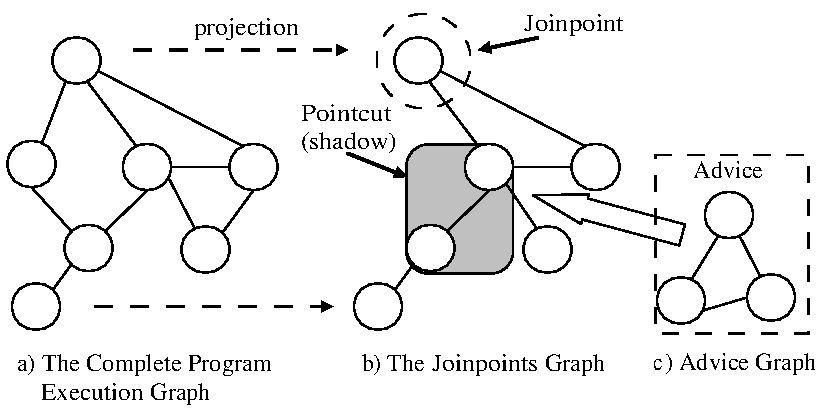
\includegraphics[width=12cm,height=!]{ch02/aop}
	\end{center}
	\caption{Illustration of Components found in the AOP Terminology}
	\label{fig:ch2aop}
\end{figure}

\begin{itemize}
\item A program is seen in AOP as an \textit{execution graph} \cite{aop.modeling.03}. A node in this graph represents a possible state of the program and an edge represents a transition from one state to another. The node set of the execution graph of a program includes theoretically any state in a program execution, with all possible paths to that state from the other states as shown in part (a) of \fig{fig:ch2aop}.

Building the complete execution graph for any arbitrary program and any possible input is unfeasible. The term \textit{execution graph} is often used in AOP to mean some abstraction of the entire execution graph, consisting of some representation of the Abstract Syntax Tree (AST) and eventually augmented by information from additional static or dynamic analysis, e.g.: data flow information, control flow information, and other forms of execution history. Collecting the additional information, e.g., execution history, may require special run-time support\footnote{An optimization used in  AspectJ \cite{www.aspectjt} is to simulate part of execution to collect some run-time data from the static AST to avoid the overhead of run-time support, for example, when implementing \textit{cflow}.}.

\item Accessible points of the execution graph are called \textit{joinpoints} and are defined as \textit{"any identifiable execution point in a system"} \cite{Laddad.aop}.
%
As shown in part (b) of \fig{fig:ch2aop}, joinpoints are a subset of the execution graph accessible in a particular representation of it\footnote{A projection in time and space of the execution graph.}. A joinpoint model describes the execution graph nodes based on the context where they are found, shown as edges inside the dashed circle in part (b) of \fig{fig:ch2aop}. That is, the execution nodes are identified not only by their own characteristics, e.g., a method signature, but also from the context where they exist, e.g., where the method is being called.

As mentioned in \sr{ch2:inv}, the accessible points of a program graph depend on the technology used to describe it. Some systems, such as AspectJ, place further restrictions on accessible joinpoints and distinguish between all possible joinpoints (accessible for example thought AST) and \textit{exposed} joinpoints \cite{Laddad.aop}. For example, AspectJ's joinpoint model does not expose loops. That is, loops are a possible, but non-exposed joinpoint.

\item An execution graph is a state machine. To modify the execution graph, there should be a way to select sets of nodes of interest and modify, replace, or delete them. There are two ways how this can be done and both are explored in AOP:

\begin{enumerate}[i.]
\item The execution graph is totally known\footnote{This is of course not possible all the time, especially at run-time.}. That is, the entire state machine graph, or at least the wanted parts to change, are known. In this case, it can be spoken of \textit{selection} of nodes and of explicit \textit{search} over the execution graph. Depending on the execution graph representation, many transformations are possible in this total view. For example, often the AST is used as a representation of the total execution graph.
 \item The execution graph is partially known at run-time. Transformations over the total view of the execution graph cannot be done in real-time. This could be a problem for those graph transformations that rely on information that is available only at run-time. In this case, the execution graph can be seen as an automata, and the transformation process can wait for patterns of transitions to appear, or \textit{events}. Every time an event happens, a respond to it in real-time with predefined \textit{event handlers (callbacks)} can be programmed.
\end{enumerate}

The real-time processing of events\footnote{That is, responding to the events as soon as they happen with the allowed timespan.} requires some form of run-time support which is often not acceptable, because of the additional overhead, or proprietary technology additions. Using partial evaluation \cite{jonesetal.93} (partial execution) techniques, many real-time (dynamic) events can be equally expressed statically, by using the information found in total static models, such as the AST, the way AspectJ does. The total view of the graph is preferable, as it removes the need to maintain the execution context. The real-time partial view requires maintaining the execution context explicitly\footnote{This is analogous to the difference between DOM and SAX parser models for XML documents (http://www.w3.org/) \cite{mcl.01}. A \textit{Dynamic Object Model (DOM)} parser processes entirely an XML document and builds a total tree of its nodes, so the node tree can be explicitly searched and modified using XPath or XQuery. A \textit{Simple API for XML (SAX)} parser, on the other hand, generates events (that can be processed as necessary) every time it encounters a node tag in a XML document. In the SAX parsers case, the context, where a node is found with regard to the other nodes, needs to be maintained explicitly when needed.}.

AOP systems logically use the real-time event-based way for reacting to sets of nodes of interest. Practically, most events can be statically implemented. For this reason, some of the early AOP systems, such as AspectJ, speak about \textit{virtual events} over the program control flow \cite{Laddad.aop}. Newer implementations, especially those of dynamic AOP, such as Prose \cite{prose}, react to actual events in the program execution and the distinction between virtual events and event-driven (triggered) systems is blurred. 

The event patterns of interest, over the execution graph, are made declarative by using specialized predicates. A predicate model could support the composition of primitive predicates. Predicates can be made part of a general-purpose language, and are known in AOP as \textit{pointcuts}. For example, pointcut predicates, such as \textit{cflow}, are made part of the AspectJ syntax. The selection criteria in a pointcut is based on all characteristics of a joinpoint, this includes a node in the execution graph and its context.

\item Every time an event of interest is matched by a pointcut predicate, some action of interest (event handler) can be executed. This is known as \textit{advice} in AOP and is shown in part (c) of \fig{fig:ch2aop}. The execution graph regions matched by a predicate are also known as the \textit{pointcut shadow} \cite{aop.semantics.02}.

The advice contains code to be executed for the matched nodes. The modifications that the advice code can do to the execution graph can include any graph rewriting \cite{mens.99} technique, depending on the model used to present the execution graph.

The process of injecting the advice code into the pointcut shadows is known as \textit{weaving}. Depending on the AOP system the weaving process can be either static or dynamic.

\item The combination of pointcuts and advice is known as an \textit{aspect}. Depending on the particular system, an aspect may contain also other elements. For example, AspectJ aspects contain compile-time directives for errors, introduction (invasive changes in the structural hierarchy of a program), and can declare new methods and fields. 
\end{itemize}

\subsection{AOP as a Generic Invasive Transformation Technique}
\label{sec:aop-inv}

The above discussion about AOP shows that AOP engines are generic transformation engines, that can be used to carry out a great range of invasive transformations. AOP techniques have been used to support product-line variability \cite{foa-aop.04,framed.aspects}. The possible AOP transformation are limited only by the joinpoint model supported by a specific AOP engine implementation. The use of generic AOP engines, such as AspectJ, is preferable for program transformation because of:

\begin{itemize}
\item \textit{Language integration}. AspectJ is tightly integrated with the Java language. This enables a great range of compiler-based static checking to find errors in the aspect code\footnote{AspectJ is not the only generic generative framework that is statically checked.}.
   
\item \textit{Declarativenes}. AspectJ offers a set of declarative context-enabled predicates (pointcuts) to select nodes of interest\footnote{AspectJ users are not explicitly aware that aspects rely on the meta-model of a program to manipulate it. This is explicit in other systems with meta-programming capabilities.}. The pointcuts not only ease the implementation, they also build a common vocabulary to speak about node selection.
\item \textit{IDE support}. Statically checked generative tools with IDE\footnote{Integrated Development Environment.} support simplify the implementation of program transformations. AspectJ is tightly integrated to Java, and well supported by development tools, such as,  Eclipse AJDT \cite{Eclipse.AJDT}.
\end{itemize}

These features make any generic transformation system, such as AspectJ, preferable, because the cost of developing custom transformation systems is often high and cannot be justified. There are also several liabilities:

\begin{itemize}

\item \textit{Specialized transformation engines can explore better the domain characteristics.} Generic transformation engines, including the AOP ones, are not always the best option. Generic transformation engines could be used to implement transformations in those systems where it makes no sense to invest in a more specific transformation technology. However, invasive transformation frameworks specialized for a narrower purpose are better suited in the long term than any generic transformation engine. An example, where a specific technique is better suited than any generic technique, would be to add OO support to ANSI C. Starting with a C \texttt{struct} construct, additional abstractions around it could be defined, using a combination of C code and generative transformations as in \cite{ooc}, to make the \texttt{struct} construct behave as a C++ class. Any invasive transformation tool that allows us to access the AST of a C program can be used for this purpose. However, the complexity of the solution would make any generic tool based implementation complex. Specialized generative techniques for this problem, as in \cite{ooc}, work better in ANSI C case. And it is even better, when the OO abstractions are made part of the language, as they are in C++.

\item \textit{Limitations in transformation capabilities of generic systems.} Another issue with generic transformation engines is their transformation limitations. The limitations are unfortunately not always clearly stated. For example, the joinpoint model of AspectJ cannot be used to enforce capital name conventions \cite{aop.paradox.03}. These limitations exist on purpose in AspectJ. They make its programming model simpler and AspectJ was originally intended to make various modularization factorizations over the meta-model of a Java program easier. Supporting very detailed joinpoint models is possible, but would remove much of the declarativeness of the pointcut notations used. 

\item \textit{Limited support for vertical transformations.} AOP engines, such as AspectJ are tightly connected to the meta-model of the language they target. They cannot support new keywords or new language constructs. This makes some generic AOP systems, such as AspectJ, to offer limited support for implementing arbitrary DSA constructs. \Sr{sec.aop.dsa} returns to this issue and explains in more detail the relation between AOP and DSA.

\end{itemize}

\noindent \Kr{ch04} develops a transformation technology specialized for interpreting DSA emulated with attributes. Having a special transformation technology for this domain, enables developing modular attribute-driven transformers that are difficult to structure and enforce with more generic transformation technologies. It makes sense to invest on an attribute-driven transformation technology, as the problem is relatively complex,  very specific, and the attribute-driven transformation technology can be used to support open container frameworks to organize assets of product-lines for more than one domain. %In AOP terms, the domain-specific modularizations of \kr{ch04} specialize the organization of the advice code.

\cendsection{Chapter Summary}
\label{ch2sum}

%Several technologies exist for the mobile device application development. Virtual machine abstractions, e.g., J2ME MIDP, hide the complexity of the underlying hardware and specific operating systems. Developing automation mechanisms for specific mobile domains can help to further reduce the costs of mobile device applications.

More mobile device applications can be build and debugged in time, when product-lines are introduced. Iterative mobile application product-lines automatically reuse the common functionality of the mobile application families. Several variability mechanisms can be used to support mobile product-lines, e.g., OO libraries, frameworks, visual modeling with CASE tools, and domain-specific abstractions (DSA). 

DSA support the architecture of a mobile product-line at the language level, blur the architectural distinction between visual CASE tools and programming language constructs, and allow for domain-specific optimizations. The cost of introducing DSA remains still very high, and low-cost implementation mechanisms need to be explored. 

Software containers offer an convenient architectural pattern to organize product-line assets. Containers clearly separate the application specific functionality from the cross-cutting domain functionality. Containers can be used to transparently inject the domain services into a specific application. A mobile container is used to support product-lines for mobile device applications. The assets of a mobile product-line are organized as container services, having both a server and a mobile client part. DSA, combined with the container abstraction, can be used to create open container families for supporting iterative product-line development.

There are several invasive and non-invasive approaches to implement the dependency injection of services in containers. Non-invasive techniques are easier to implement, but offer less automation. Invasive techniques are better suited to support attribute-based DSA in mobile containers. Static invasive techniques, in the context of a container, can be used to bind the attribute-based DSA to the product-line services.

The need for several technologies was identified, that will be explored further in the following chapters:

\begin{itemize}
\item \textit{Lightweight language extensions based on attributes.} Attribute enabled language tech\-no\-lo\-gy can be used to emulate embedded DSA. Attributes support iterative product-line development with minimum start-up costs. Language technology that directly supports attribute-based transformations is needed \seec{ch03}.

\item \textit{Attribute-driven transformation support.} Any generic invasive programming technology can be used to implement and support attribute-based abstractions. Specialized transformations could help to better modularize attribute-based transformers and make them declarative. Attribute-based transformer technology enables the reuse of transformation components and declarative composition of attribute-based transformers \seec{ch04}.

\item \textit{Open container families.} Extensible containers are needed to organize the common mobile device application functionality. Mobile containers are specialized to address the peculiarities of mobile applications and to organize the mobile product-line assets, such as, the need for data adaptation \seec{ch05}.

\end{itemize}

%ch03.tex

%\pagestyle{headings}

\chapter{Attribute Enabled Software Development}
\label{ch:gaast}
\label{ch03}
\mquote{We don't usually consider a statement to be data at
all, since it cannot be read, written, or manipulated.}{R. A. Finkel, Advanced Programming Language Design, 1996}

\noindent This chapter\footnote{This chapter shares content with references \cite{cepa.mezini.gaast.04,cepa.kloppenburg.05}.} explains the main ideas behind attribute-enabled language technologies\footnote{The term \textit{language technology} is used to mean the complete language system: the grammar, the binary representation, and the run-time system.} and their usage to sustain domain specific abstractions (DSA). \Sr{c2.sec.dsa.attributes} portrays how DSA can be supported with attributes, and how the domain variability can be modeled as nested attribute-families. The advantages of \textit{attribute enabled programming} (AEP) are discussed in \sr{sec:gaast-mda}, by analyzing several scenarios for mapping of Model-Driven Architecture (MDA) UML class diagram models onto source code artifacts. %Several widely used approaches for mapping MDA models are compared with the attribute programming.

\Sr{sec:problem-statement} investigates several ways to support the attribute-based software design in UML class diagrams. The language technology behind AEP is discussed in \sr{sec:gaast}, stressing the importance that this technology be part of the core language, and supported by the language vendor. Related approaches are addressed in \sr{sec.related.dsl}. Attribute programming is compared with other ways to support EDSL constructs, namely extensible grammars / compilers and meta-programming systems. Finally, \sr{sec.attribute.usage} explores the proper usage of attributes to clarify the power and some of the pitfalls of the AEP.

\begin{figure}[ht]
%	\begin{center}
	  \xymatrix{
	  *+[F]{\txt{Supporting DSA with Attributes \\\Sr{c2.sec.dsa.attributes}}} \ar[r] \ar[d] \ar[dr] &
	  *+[F]{\txt{GAAST Languages \\\Sr{sec:gaast}}} \ar[d]
	  \\
	  	*+[F]{\txt{Advantages of Attribute Programming \\\Sr{sec:gaast-mda}}} \ar[d] \ar[dr] & *+[F]{\txt{Comparison to other Approaches  \\\Sr{sec.related.dsl}}}\\  	
*+[F]{\txt{Representing Attributes in UML \\\Sr{sec:problem-statement}}}  	 & *+[F]{\txt{Proper Usage of Attributes \\\Sr{sec.attribute.usage}}} \\  }
%	\end{center}
%	\caption{Chapter Overview}
%	\label{fig:contents}
\end{figure}

\section{Supporting DSA with Attributes}
\label{c2.sec.dsa.attributes}

Based on the third alternative for implementing domain specific abstractions (DSA) explained in \sr{sec:var.dsa}, namely generic language extensions, this book presents technology that addresses the DSA drawbacks mentioned in \sr{sec:var.dsa}, based on \textit{explicit attributes} \cite{hedin.97,java.explicit.programming}. Explicit attributes are a lightweight language extension which reduces the grammar processing costs, and the accidental \cite{brooks.87} costs of the DSA implementation.
%
Using a \textit{attribute} (or \textit{tag}) to denote an additional property about an existing entity is intuitive. When Knuth \cite{knuth.90} describes the idea of using attributes as tags that carry out semantics related to grammar productions, he notes that the idea has been around for some time. Since then, attribute grammars have evolved and matured and they are used in different ways to develop software \cite{attrib.gram}.

\begin{figure}[ht]
	\begin{center}
		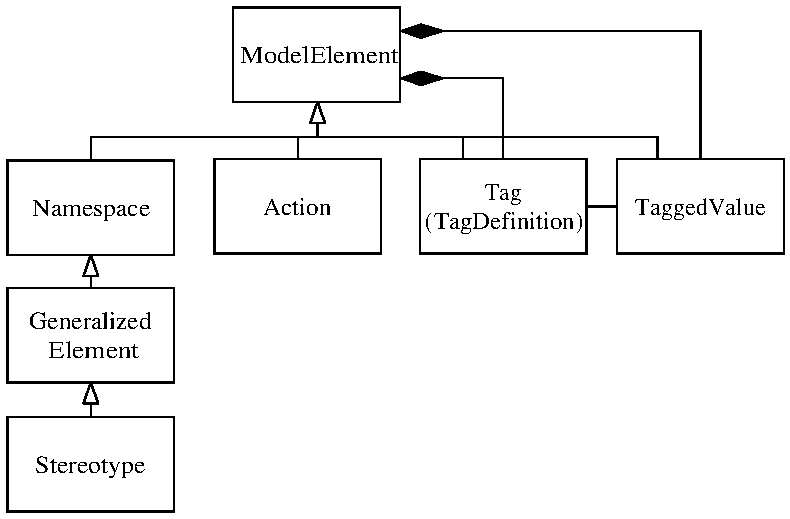
\includegraphics[width=!,height=5cm]{ch03/mof-uml-tag}
	\end{center}
	\caption{The \textit{Tag} element in MOF / UML can be used with any \textit{ModelElement}}
	\label{fig:mof-uml-tag}
\end{figure}

An example is the tag definition and usage in the Meta-Object Facility (MOF) \cite{www.mof} and the Unified Modeling Language (UML) \cite{www.uml}\footnote{UML can be described in terms of MOF.}. In MOF, tags derive from the class {\tt Mo\-del\-Ele\-ment}, i.e., any element can be decorated with custom defined tags (\fig{fig:mof-uml-tag}). Tags carry no domain-specific semantics for the MOF or UML itself. Their semantics are meaningful only to the modeler of the profile, who introduces the tag definitions. Tags serve as hints to model transformers and generators \cite{mda.frankel}, and enable the association of arbitrary semantics with model elements of interest, without having to change the meta-model of a given model. In terms of MOF, tags enable modeling in different vertical layers simultaneously. There is some functionality available to modify the meta-model M$_{i+1}$ in the layer M$_{i}$, providing similar functionality in the layer M$_{i}$, as found directly in the upper meta-model layer M$_{i+1}$. 

This book focuses on the usage of \textit{attributes} \cite{www.dotnet}, known also as \textit{annotations} \cite{www.java.meta}, or \textit{tags} \cite{www.mof}, as a form of graph labeling \cite{term.rewrite,Plump.95,mens.99} at the programming language level\footnote{Different names are used for tags, such as attributes \cite{www.dotnet} or annotators \cite{www.java.meta}.}. In some programming languages, attributes are \textit{explicitly} present as part of the grammar rules, and enable modification of the semantics of the language constructs without changing the grammar \cite{Taha.1997}. The interest is in programming languages that enable a programmer to define any number of attributes to decorate selected elements, promoting an explicit attribute programming model \cite{java.explicit.programming}. Examples of languages that support the annotation of program elements with attributes are the .NET \cite{www.dotnet} platform with its common language model, and Java 1.5, whose annotations support is described in JSR 175 \cite{www.java.meta}. In other languages, where support for attributes is missing, e.g., J2ME MIDP \cite{www.midp-ota}, attributes can be emulated with special comments, as is the case with JavaDoc \cite{jw-pollac} comments in Java 1.4 \seec{ch05}.

Unlike other approaches, where a limited number of predefined attributes is used to replace custom keywords \cite{Taha.1997}, explicit attributes can be introduced freely, in any number, in a language that supports them. They are used directly at the source level and hence the qualification \textit{explicit}. This is different from other approaches, where attributes are used in the inner parts of a compiler to save intermediate processing results \cite{asfsdf.02,java.compilers.book}. Attributes enable the decoration of program entities with custom notations, whose semantics are defined by the programmer. Attribute decorations are explicitly used by the developers and represent semantics that make use of an arbitrary context, unlike in an attribute grammar \cite{attrib.gram,morr.02}, where attributes are used inside the parser to help with the evaluation of the grammar rules, having with a well-defined context propagation. Attributes can be parameterized \see{ch03:sec:attrib.param} and help to drive program transformations. 


Attributes can be used to emulate DSA at the language level. In a language that supports attributes, e.g., .NET C\# \cite{www.dotnet}, the same web service language extensions of \fig{fig:webservice-dsl} \see{sec:var.dsa} can be coded by introducing two custom attributes, as illustrated in \fig{fig:webservice}.
The \texttt{Travel\-Agent} class is decorated with a \texttt{[Web\-Servi\-ce]} attribute, whereas its public methods that constitute the web service interface contain a \texttt{[Web\-Me\-thod]} attribute. Introducing new attributes is supported directly by the .NET compilers. There is no need to deal with any grammar modification issues, making it easier to extend a .NET-based language, such as C\#, with domain-specific constructs.

\begin{figure}[ht]
\begin{center}
\begin{minipage}{7cm}
\begin{scriptsize}
\begin{lstlisting}[numbers=left,language=Java,frame=leftline]{}
[WebService]
class TravelAgent {
  ...
  [WebMethod]
  public void GetHotels(){...}
  ...
}
\end{lstlisting}
\end{scriptsize}
\end{minipage}
\end{center}
\caption{A Web Service Class with two Inter-depended Attributes}
\label{fig:webservice}
\end{figure}

Unlike some other forms of EDSLs, such as SQLj \cite{www.sqlj}, which introduce islands of alien code into a host language, the methodology presented in this book is restricted to less expressive language extensions in the form of new parameterized attribute-based keywords, that fit in the overall design of the host language. While less expressive than full-fledged EDSLs, attribute-based language extensions are expressive enough to support declarative DSA for iterative product-line variability, as will be explained in \sr{sec.related.dsl} and demonstrated in \kr{ch05}. The attribute technology makes it possible to benefit from the declarative nature of DSA in order to preserve the domain abstractions, whereas at the same time, attributes keep the start-up costs of DSA extensions at a minimum. These features makes attribute-based DSA a variation mechanism of choice for iterative mobile product-lines.


\subsection{Supporting Domain Variability with Attribute Families}
\label{attribute.families}

There are several techniques to identify the core assets and to present the variability of the requirements for a domain \cite{Requirements.Engineering}. One of the most widely used is Feature-Oriented Domain Analysis (FODA) \cite{foda.90,generative.00,foda.sem}. FODA models variability as feature trees with required, optional, or alternative sub-trees. Starting with a feature diagram, it is possible to identify components of a system and produce design models of how the final system may look like \cite{foda.uml1}. Feature representation facilitates also the representation of the domain concerns with declarative programming constructs \cite{foda.dsl}. Modeling of the domain features with attributes could follow the structure of the feature diagrams.

\begin{figure}[ht]
	\begin{center}
		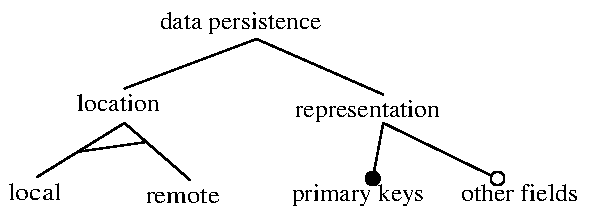
\includegraphics[width=10cm,height=!]{ch03/foda}
	\end{center}
	\caption{Feature Representation of Data Persistence}
	\label{c3fig:foda}
\end{figure}

The idea is to model the top features of a domain, that would be handled by an attribute-based container, by using single attributes. For example, a single attribute can be used to represent a top-level feature, such as the need to persist the data in a mobile application. A simplified (non-complete) feature model of data persistence is shown in \fig{c3fig:foda}. The data may need to be stored locally in the device, or remotely on the server-side. The possible representation model of the data needs to be decided for each component, e.g., to identify the fields that will serve as primary keys. Similarly to a feature model, attributes can be grouped in tree-like name spaces, where each name space is used to model different parameters of a single product-line asset. Sub-attributes are added as necessary to follow the feature model, and obtain a tree-like view of the modeled domain concerns. Attribute name spaces will be called \textit{attribute families}, and a C++ \cite{cpp.97} namespace-like dot notation will be used to organize them. The parameterization of attribute families is done by using nested attributes, or attribute parameters.

\begin{figure}[ht]
\begin{minipage}[t]{0.5\linewidth}
\begin{center}
\begin{scriptsize}
\begin{lstlisting}[numbers=left,language=Java,frame=leftline]{}
[dp]
[validate]
[property]
public class GameScore {

  [dp.pk]
  [dp.pk.sort("asc")]
  [validate.min(0)]
  [validate.max(100)]
  [property.accessor]
  private int score;

  [dp.pk]
  [dp.pk.sort("asc")]
  [validate.min(4)]
  [validate.max(32)]
  [property.both]
  private String playerName;

  [property.both]
  private String Comment;
}
\end{lstlisting}
\vspace{1.75cm}
\end{scriptsize}
\end{center}
\caption{Input Code}
\label{fig:input}
\end{minipage}%
\begin{minipage}[t]{0.5\linewidth}
\begin{center}
\begin{scriptsize}
	\begin{lstlisting}[numbers=left,language=Java,frame=leftline]{}
public class GameScore {
  private int score;
  private String playerName;
  private String Comment;

  public getScore() { return score; }
	
  public String setPlayerName(
    string value)
  { playerName = value; }
	
  // ...
  public byte[] toRecord()
  {
    ByteArrayOutputStream baos =
        new ByteArrayOutputStream();
    DataOutputStream outputStream =
        new DataOutputStream(baos);
    outputStream.writeInt(o.getScore());
    outputStream.writeUTF(
        o.getPlayerName());
    outputStream.writeUTF(
        o.getComment());
    return baos.toByteArray();
  }
  // ...
}
\end{lstlisting}
\end{scriptsize}
\end{center}
\caption{Output Code}
\label{fig:output}
\end{minipage}
\end{figure}

For example, consider the attribute-based implementation example of a \textit{GameScore} component in a mobile application\footnote{The example is based on the standard \textit{GameScore} example which comes with J2ME MIDP 2.0 \cite{www.midp-ota} documentation, explained in \kr{ch05}. The examples of  \fig{fig:input} and  \fig{fig:output} will be reused in \kr{ch04} to explain attribute-driven transformations.}, shown in \fig{fig:input}. The code in \fig{fig:input} is a declarative specification of the functionality encoded in \fig{fig:output}\footnote{The code in \fig{fig:output} is one possible result of mapping the code in \fig{fig:input} to a concrete implementation for a concrete mobile device.}. The fields in \fig{fig:input} are decorated with explicit attributes in the form of special \texttt{'[]'} comments. The following attribute families correspond to the different generic domain assets \see{c2.container.domain} that have been used in the code of \fig{fig:input}:
\begin{itemize}
\item \texttt{[property]} - adds accessor / mutator methods for a field (lines 3, 10, 17, and 20).
\item \texttt{[validate]} - adds validation code for fields that have mutator methods; \textit{min, max} show the required range for an integer or the required length ranges for a string field (lines 2, 8, 9, 15, and 16).
\item \texttt{[dp]} - adds data persistence methods to the component, and enables retrieving the data records sorted based on the primary keys (presented as an attribute sub-family \texttt{dp.pk}) (lines 1, 6, 7, 13, and 14).
\end{itemize}

The organization of attribute families is similar to organizing other language abstractions into name spaces and enables the reuse of attribute names with overloaded semantics, reducing the total required vocabulary. For example, all attributes related to the persistence of data in a device start with the \texttt{db} prefix (lines 1, 6, 7, 13, and 14 of \fig{fig:input}). Attribute parameters, e.g., \texttt{"asc"} in line 7 of \fig{fig:input}, are used to support the variability of the specific attributes inside an attribute family. Attribute families provide a convenient method to organize the domain functionality. All domain assets are organized as a tree of attribute families. Similar to language name spaces, attribute families can contain nested sub-families that group the variability of similar concepts, e.g., \texttt{db.pk}, groups the variability parameters related to the primary keys (lines 6, 7, 13, and 14 of \fig{fig:input}).

Based on the domain features, the architectural space of a product-line can be designed and its programming model can be decided. In \cite{generative.00}, the domain features are divided in four classes: concrete, aspectual, abstract, and grouping. As explained in section \see{c2.container.domain}, the container-based view of a product-line enables a uniform treatment of generic and specific assets and their features. The programming model can be represented by attribute families. Attributes enable a uniform representation of all the feature groups distinguished in \cite{generative.00}. For example, the concrete implementation of the data persistence feature of \fig{c3fig:foda} will be a \textit{concrete} component as part of the product-line services. The instantiation of the data persistence feature is, however, \textit{aspectual}. The specification of the primary keys needs to refer to a particular component implementation. Attributes connect the feature-based variability, implemented as part of the product-line services, with the fine-grained feature variability code written manually by the developers.

Ideally, attribute families enable the presentation of the domain features declaratively, without giving any clues about the implementation details of a given feature. In practice, the level of abstraction modeled by an attribute family is as good as the feature model used to create it. Attribute can also quickly reflect the evolution of a feature model. As explained in section \see{sec:gaast}, attribute-enabled languages offer a lightweight mechanism to support the evolution of the declarative constructs in code. 

\subsection{Attribute Parameters}
\label{ch03:sec:attrib.param}

Attribute parameters are a convenient mechanism to specify the domain variability, modeled by using attributes. This section discusses how attribute parameters can be included formally in the overall attribute model. The discussion hitherto has assumed that attributes have the following EBNF \cite{Parsing.Techniques.90} form: {\tt attributeName :=\- (paramterName =\- pa\-ra\-me\-terVa\-lue)*}. An attribute is identified by a name and by any (optional) parameters that it takes.

A distinction can be done between \textit{structural} attribute parameters that are known at compile time (usually static constants), and \textit{behavioral} parameters whose value can be determined (dynamically) only at run-time. When attributes are used for generation, they can contain only compile time evaluated parameters. Run-time evaluated parameters usually need some form of run-time support. Behavioral parameters are similar to introducing additional method / constructor arguments, and can be handled as such in the systems that need them.

When speaking about attributes, their structural parameters will be implied without making any special assumptions about them. Using parameters is only a convenience in using tags for annotations. While parameters help to express attribute variability more declaratively, they do not make annotations more powerful as summarized formally by the following theorem:

\begin{theorem}
\label{theo:tagParam}
Tags with explicit structural parameters can be always replaced with tags without parameters in a given program.
\end{theorem}

\noindent Proof: Let T be a tag and $\pi$ its parameters vector. It should be proved that (i) there exists a discrete function F: (T, $\pi$) $\to$ T', that returns a new tag T' based on the tag T and its parameters $\pi$ and (ii) that F is a finite function, that is, it has a finite co-domain. Indeed:\\
(i) Let F: (T, $\pi$) $\to$ T' be a function constructed by expressing all the parameters $\{\pi\}$ as strings that are joined together with some string separator (e.g: '\$'), and appended to the tag T, for example T' = T\$$\pi$. The function F returns a unique tag for any tuple (T, $\pi$). If '\$' is escaped inside T and $\pi$, then F has also an inverse function F$^{-1}$: T' $\to$ (T, $\pi$).\\
(ii) The function F is a total function over $\{\pi\}$. If $\{\pi\}$ is an infinite set then so is F. But the number of structural elements in a given program is finite. Thus, even though $\pi$ could be infinite, only a finite set of its values are used in a given program. So, F can be replaced with a finite set of partial functions over $\pi$ (QED).

\subsection{Connecting Attribute DSA with Product-Line Assets}
\label{dsa.connect}

Representing DSA with attributes in code removes the costs related to the grammar modification. Attribute-based DSA should, however, be interpreted and properly connected to product-line services. For example, the code in \fig{fig:inject} shows the attribute-decorated \texttt{Ga\-me\-Score} class of \fig{fig:input}. The used attributes state that the \texttt{Ga\-me\-Score} objects should be made persistent in the memory of a mobile device. The persistence requirement is expressed declaratively as a set of attributes, e.g., \texttt{dp}\footnote{Data Persistence Object.} in the \texttt{Ga\-me\-Score} class definition.

\begin{figure}[ht]
	\begin{center}
		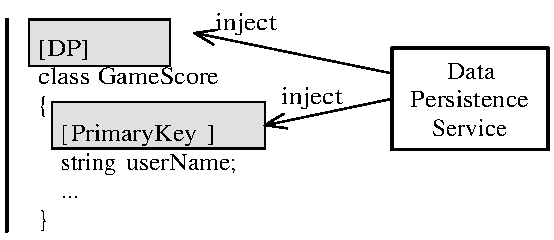
\includegraphics[width=8cm,height=!]{ch02/inject}
	\end{center}
	\caption{Connecting Attributes with Services}
	\label{fig:inject}
\end{figure}

The declarative attribute-based DSA notation needs to be connected to the actual data persistence code (service). The connection can be implemented in a variety of ways, for example by enhancing the compiler to detect and process the attributes, or by using some other way to organize services, such as, as component libraries or templates, and then bind them to the attribute-decorated code as required. Given that the focus is on easy to implement and to maintain DSA mechanisms, extending the compiler is not an option.

\Sr{c2sec:containers} already discussed how product-line assets can be organized as services that are transparently managed by a software container abstraction. \Kr{ch04} develops a technology to implement modular attribute-based transformers, which helps to develop low-cost attribute-based DSA transformations and connect them to the product-line services. Attributes can be interpreted before, or after compilation, or at runtime. Attribute interpretation requires to somehow be able to access and eventually modify / transform some AST-like source- or binary-level representation of the annotated program. For instance, tags used in MOF / UML can be interpreted when the model is transformed to another more detailed model. JavaDoc attributes used in Java 1.4 can be interpreted when the source code is processed. .NET attributes, or Java 1.5 annotations are saved as part of the binary meta-data. This enables the manipulation of binaries after compilation, or the run-time interpretation of tags by using the Reflection API. The run-time interpretation requires that the original annotated program is structured in such a way, that it can be compiled without interpreting the tag semantics. For example, in .NET a method body cannot use a variable that will be introduced by an attribute interpretation, because such a method cannot be compiled.

This chapter concentrates on language technology for supporting and facilitating the construction and maintenance of attribute-based DSA transformers. Before doing so, in order to complete the attribute-based software development (AESD) discussion, the advantages of AEP will be summarized, and ways to integrate attributes in the early phases of software development will be considered.

\section{Advantages of Attribute Programming}
\label{sec:gaast-mda}

This section compares the benefits of having access to explicit attribute support at the language level, with other techniques to model domain abstractions in source code, namely marking interfaces and pseudo-syntax marking. A typical model mapping scenario from \textit{Model-Driven Architecture} (MDA) \cite{mda,mda.frankel} is used. The goal of MDA is to increase the level of abstraction of software development. MDA enables software developers to specify "what" a software solution should provide, rather than "how" to realize the desired solution in terms of the technicalities of a particular implementation platform. The "what" is specified in a so-called \textit{Platform Independent Model} (PIM). Based on the chosen technology, there are different operations that can be used to realize a PIM, resulting in different \textit{platform specific models} (PSMs) of the same PIM. A PSM can be a ready-to-run implementation, or it may act as a lower-level PIM for further refinement to a new PSM that can be directly implemented.

Obviously, it is desirable to have an abstract PIM and to automate its translation to a given PSM implementation. A fully automatic transformation of any abstract model is not possible. Additional PSM specific directives need to be provided by applying marks from a specific profile\footnote{UML profiles modify the UML M2 model, i.e., they bring extensions to the M2 level.} to PIM elements. This implies a commitment to some kind of specific technology for solving the problem. The profile denotes the domain-specific notations, by using specialized forms of marking, e.g., tagged values and stereotypes. Marking represents concepts of the PSM in the PIM and indicates how the PIM elements are to be transformed \cite{mda.guide}. 

For illustration, \fig{fig.uml1} shows a simple web service with two methods, (i) to log in and authenticate a client (user) ({\tt Lo\-gin}), and (ii) to enable the client to access some user specific data ({\tt Access\-User\-Data}). The simple web service class, named \texttt{Web\-Ser\-vi\-ce1}, is modeled by the means of UML profiles. Three stereotypes {\tt \flqq web\-ser\-vi\-ce\frqq}, {\tt \flqq namespace\frqq} and {\tt \flqq uniqueid\frqq} are defined. The last two can also be represented as tagged values connected to the {\tt \flqq web\-ser\-vi\-ce\frqq{}} stereotype. In addition, two free tagged values, \texttt{ena\-ble\-Se\-ssion} of type \texttt{boolean} and \texttt{tran\-sac\-ti\-on\-Opti\-on} of type {\tt enu\-me\-ra\-tion}, are used to decorate the methods of this web service.

\begin{figure}[ht]
	\begin{center}
		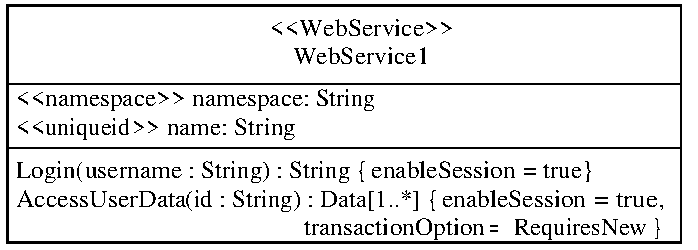
\includegraphics[width=8cm,height=!]{ch03/uml1}
	\end{center}
	\caption{Modeling using UML Profiles}
	\label{fig.uml1}
\end{figure}

Compared to a more abstract counterpart that does not contain any of the above tags, the model of \fig{fig.uml1} is technology dependent. Several technology commitments are made by using the profile. First, it is decided to expose the component as a web service. Second, the technical concerns needed by the service methods are explicitly enumerated, e.g., session and transaction management. However, at this point there is not yet any commitment made on how the session and transaction management will be implemented. The example only states the need for such technical services by means of the specialized UML profile, but has not yet committed to a particular web service platform.

In the MDA terms, the model in \fig{fig.uml1} is still a PIM for a more specific PSM. Given such a marked PIM, some transformer \texttt{T$_{1}$} is applied to produce a lower-level PSM, as shown schematically in \fig{fig.mda-model}. In MDA the commitment about the technology is done in stages rather than at once. The rationale behind this stratified commitment \cite{kuhne.01} is that a model of a higher-level stage can be mapped to more than one possible model of a lower stage. A staged commitment makes it possible to exchange the lower-level models, while preserving the investment on the higher-level models.

\begin{figure}[ht]
	\begin{center}
		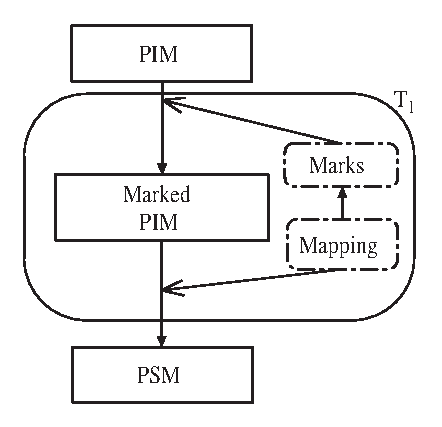
\includegraphics[width=4.5cm,height=!]{ch03/mda-model-orig}
	\end{center}
	\caption{MDA PIM-to-PSM Transformations}
	\label{fig.mda-model}
\end{figure}

Assuming that the target PSM is expressed in a programming language, the transformer \texttt{T$_{1}$} knows (a) how to map marks to corresponding language constructs, and (b) how to map types used in the model, to types of the target programming language, e.g., a \textit{String} in the modeling language may map to a character array in the target programming language. Type mapping is usually easy to handle automatically and will be not addressed any further. By selecting a given language, a further commitment is made on what the final software will be like. Selecting the target language says still nothing about how issues, such as sessions and transactions, will be implemented by tag interpretation (eventually in a later stage). Concerning the tag mapping, in the case when the target PSM (\fig{fig.mda-model}) is expressed in a concrete programming language, it could be distinguished between:
\begin{itemize}
\item mapping the tags to language constructs, and 
\item interpreting the language constructs to insert the specific concern's functionality.
\end{itemize}
  
A specific transformer may combine all three stages (mapping types, mapping marks to language constructs, and interpreting the latter) into a single pass. For instance, in addition to type and tag mapping, \texttt{T$_{1}$} (\fig{fig.mda-model}) may also interpret the tags. In this case, \texttt{T$_{1}$} commits to concrete session and transaction implementations and produces an executable PSM.

However, it makes sense to separate tag mapping from tag interpretation, when the transformation of a  PIM to an executable PSM is not fully automatic. This is the case when modeling is used only for defining the high-level architecture of an application. For example, in an EJB \cite{www.ejb} application, it is preferred to model beans and their interactions by means of UML constructs. It is easier to write and maintain complex business functionality directly in Java rather than to model {\tt for} loops and similar constructs using the UML action language \cite{www.uml}\footnote{The UML action language might be well suited to model embedded systems, where full automation of the transformation would make sense.}. In the web service example, issues, such as sessions and transactions, will be handled automatically. Programmers may still fill-in manually the functionality for logging and retrieving data by implementing the methods {\tt Login} and {\tt AccessUserData}.

As the focus is on programming language support for tag mapping and interpretation, the interest will be in lightweight mappings of tags to language constructs that do not require domain-specific additions to the target language. Such mappings are preferable because of lower costs for mapping arbitrary custom profile elements to a general-purpose language. The remaining of this section compares three widely used approaches for handling the mapping of tags to programming language constructs and for the interpretation of language constructs, namely: \textit{marking interfaces}, \textit{pseudo-syntactic marking} and \textit{attribute mapping}\footnote{A given tool may use any combination of these approaches.}. The comparison is done along the following dimensions:

\begin{enumerate}
\item \textit{Preservation of the PIM.} Preserving the architecture of the marked PIM in the source PSM is important, because it helps (a) to reverse engineer the source code PSM and (b) to understand the original PIM architecture by looking at source code alone. \fig{fig.text.1} shows an equivalent textual model of the web service of \fig{fig.uml1} in an extended\footnote{The introduced extensions address modeling profile elements. The current version of HUTN specification does not address any extension mechanisms for HUTN in order to keep the language simple \cite{hutn.dipl}.} HUTN\footnote{Human-Usable Textual Notation.} notation \cite{hutn}. The OMG HUTN standard is aimed at defining textual equivalents of MOF / UML diagrams which can automatically be generated. The tags of the web service example are modeled as extended adjectives in terms of HUTN. It is desirable that the source code PSM preserves the PIM structure to the same degree as the HUTN representation.

\begin{figure}[ht]
	\begin{center}
	\begin{minipage}[t]{8cm}
		\begin{scriptsize}
		\begin{lstlisting}[numbers=left,frame=leftline,showstringspaces=false]{}
webservice "WebService1"
{
  namespace namespace : "www.st.tu-darmstadt.de"
  uniquieid name : "Simple Service"

  enableSession Login(username : String) : String
  enableSession transactionOption.RequiresNew
    AccessUserData(id : String) : Data[1..*]
}		
\end{lstlisting}
		\end{scriptsize}
		\end{minipage}
	\end{center}
	\caption{Extended HUTN Model}
	\label{fig.text.1}
\end{figure}

\item \textit{Complexity of the Programming Model.} As already mentioned, parts of the code need often to be filled-in manually by the programmer in the generated PSM code. The structure of the PSM produced by tag mapping directly affects how the programmer interacts with such code. It is preferable to keep the programming model simple.

\item \textit{Interpretation of Mappings.} Interpretation is the next step after marks are mapped into language entities. Different kinds of mappings result in different techniques of interpretation. The interest will be in how easy it is to interpret language constructs resulting from tag mapping by considering the native support that the language technology offers for this purpose.

\item \textit{Extensibility of the Profile.} Extending a profile is often a requirement rather than an option. It is preferable to have means which facilitate the introduction of custom extensions to profiles. To illustrate the discussion, suppose that a new traceability tag named { \tt log} is added to the custom web service profile of \fig{fig.uml1}. This tag, when used with a method, will generate code that logs all method invocations. In the discussion that follows, the tag will be added to the { \tt Login} method. Logging enables to register which users used the service, at what time, and which users failed to authenticate.
\end{enumerate}

\subsection{Mapping Marked PIMs to Marking Interfaces}
\label{attributes}

To implement mapping of the PIM of \fig{fig.uml1} in Java 1.4, interfaces are often used as a means to emulate marking code elements at the language level \cite{design.attrib,mda.frankel}. When the PIM of \fig{fig.uml1} needs to be implemented in Java 1.4, it could map to the Java model consisting of the classes and interfaces of \fig{fig.uml.2}.

\begin{figure}[ht]
	\begin{center}
		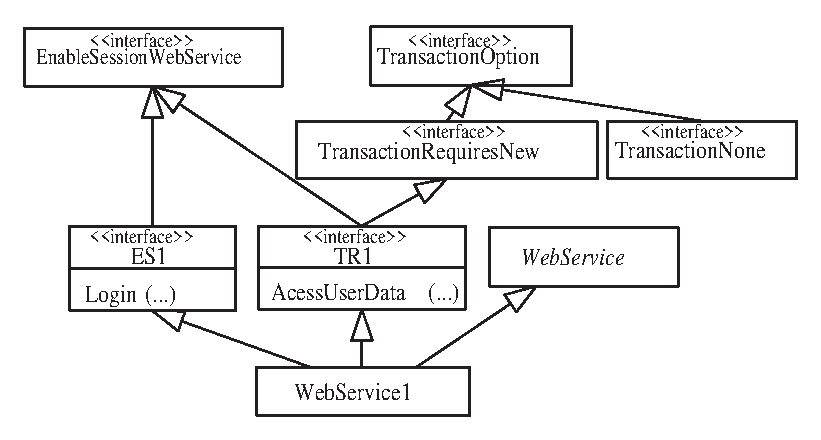
\includegraphics[width=10cm,height=!]{ch03/uml2}
	\end{center}
	\caption{Mapping by Means of Marking Interfaces}
	\label{fig.uml.2}
\end{figure}

For each tag and stereotype in \fig{fig.uml1}, a marking interface is introduced in \fig{fig.uml.2}. Multiple-value attributes are modeled as specialized interfaces that derive from other base marking interfaces. For example, \fig{fig.uml.2} assumes that the multi-value tag {\tt tran\-sactionOpti\-on} can only have two possible values, {\tt RequiresNew} and {\tt None}, which are modeled as children interfaces of the {\tt Tran\-sactionOpti\-on}. The stereotypes can also be modeled as marking interfaces, or as specialized (prototype) classes, e.g., {\tt WebSer\-vice} in \fig{fig.uml.2}. The mappings for the {\tt \flqq namespace\frqq} and {\tt \flqq uniqueid\frqq} stereotypes are not shown in \fig{fig.uml.2} and it is assumed that they are used in the implementation of {\tt WebService}. 

To emulate the tags of a given PIM method in a given class, a specialized interface for that method needs to be created. The specialized method interface derives from the basic interfaces that model the respective tags. For example, the interface {\tt ES1} inherits from {\tt Ena\-bleSe\-ssionWebSer\-vi\-ce} to make explicit that the method {\tt Login} is marked by the tag emulated by the {\tt Ena\-bleSessi\-onWebSer\-vice} interface. In the same way, the interface {\tt TR1} containing the method {\tt AccessUserData} is derived from {\tt EnableSessionWebService} and {\tt Tran\-sa\-ctionRe\-quires\-New} to reflect the fact that this method is marked by both {\tt ena\-bleSe\-ssion} and {\tt tran\-sac\-tionOption=Re\-quire\-sNew} in \fig{fig.uml1}. This way, the attributes of a method can be found by looking at the interface it belongs to.

\noindent Discussion:
\begin{enumerate}
\item \textit{Preservation of the PIM} - The mapping of \fig{fig.uml.2} does not preserve the modular structure of the PIM in \fig{fig.uml1}. From the model in \fig{fig.uml.2}, it is hard to guess the clear and concise structure and semantics expressed by the original PIM. The corresponding PSM code contains an explosive number of marking interfaces. This makes the PSM model more difficult to understand and hinders reverse engineering to the original PIM. The corresponding Java code of the UML model of \fig{fig.uml.2} will also be much more verbose compared with the textual HUTN representation of \fig{fig.text.1}. 

\item \textit{Complexity of the Programming Model} - Even though the example is extremely simple and several simplifying assumptions were done, the resulting PSM (\fig{fig.uml.2}) gets complex and verbose. Cross-interfaces need to be introduced, which inherit from base ones. The resulting PSM already mixes the business logic model with the model for implementing technical concerns. The technical concerns crosscut the modular structure of the business logic in \fig{fig.uml.2} and dictate the inheritance structure of the resulting program. The developer responsible for implementing the PSM in \fig{fig.uml.2} cannot "escape" some issues related to the implementation of the technical concerns. The developer has to know that interfaces, such as {\tt ES1}, exist and will be handled by a suitable concern automation environment.

\item \textit{Interpretation of Mappings} - Marking interfaces are not easy to interpret. Extracting the tags of a given method requires finding the interface where the method is declared, and retrieving the interfaces from which this interface inherits. When the interpretation is done at the source-code level, the full inheritance hierarchy must be resolved. Using compiled pseudo-binaries that contain meta-data, e.g., Java bytecode along with the Reflection API, makes it easier to resolve marking. Reflection relies on the existing virtual machine mechanisms to resolve the inheritance hierarchy. In order to extract knowledge about the marking interfaces hierarchy, the transformer that performs the mapping of marks must know the meta-model abstractions of the marked PIM. 

The overhead of tag extraction in terms of both complexity and performance of the interpretation logic cannot be avoided because the mapping of model tags to programming language constructs does not preserve tags as first-class values. First, as indicated above, the transformer that maps tags to language constructs is complex and needs to know the tag meta-model of the marked PIM. Second, the tag interpretation transformer needs to basically "undo" this work in order to extract tags from the marking interfaces resulting in a double overhead.

\item \textit{Extensibility} - To add a new {\tt log} tag to the method {\tt Login}, a new additional interface {\tt Log} need to be created in the language representation. In addition, the {\tt ES1} interface needs to be modified so that the web service class inherits from the new interface, in order to make explicit which new attributes the {\tt Login} method has. If {\tt log} were to be added to the other methods, the other interfaces need to be modified in a similar way. This would make the PSM model even more complex. Hence, the marking interfaces approach does not scale well. 
\end{enumerate}

\subsection{Mapping Marked PIMs to Pseudo-Syntactic Elements}
\label{ch03.pseudo.syn}

One way to decrease the number of the resulting marking interfaces is to rely on coding conventions, such as those used  in JavaBeans \cite{javabeans}, J2EE EJB \cite{www.j2ee}, or COMPOST \cite{java.compost}. Pseudo-syntactic marking uses string prefixes / suffixes to decorate the names of the marked elements according to some accepted convention based on the marked PIM. This approach will be called \textit{pseudo-syntactic marking}, because it adds new syntax to a language without really adding new keywords. 

Some systems, e.g., COMPOST \cite{java.compost}, rely on pseudo-syntactic marking for expressing class and member annotations. Other systems, e.g., JavaBeans \cite{javabeans} and J2EE EJB \cite{www.j2ee}, use a mixture of marking interfaces, required coding conventions, and annotations defined in so-called bean info objects (in the XML deployment descriptor). J2EE EJB implements class-level annotations by means of predefined classes / interfaces from which the annotated classes inherit. For methods and attributes, JavaBeans and J2EE EJB use pseudo-syntactic marking.
 
\begin{figure}[ht]
\begin{center}
\begin{minipage}[t]{8cm}
	\begin{scriptsize}
\begin{lstlisting}[numbers=left,language=Java,frame=leftline]{}
WebService1 implements WebService {
   String sessionLogin(String username) { ... }
   Data[] session_transactionAccessUserName(String id) {
     Transaction t = 
       context.getTransactionFactory().NewTransaction();
 	    ...
   }
}
\end{lstlisting}
	\end{scriptsize}
	\end{minipage}
\end{center}
	\caption{Using Pseudo-Syntactic Marking}
	\label{fig.pseudo-marking}
\end{figure}

For illustration, \fig{fig.pseudo-marking} shows how the web service of \fig{fig.uml1} could be mapped with pseudo-syntactic marking.
The {\tt \flqq Web\-Ser\-vi\-ce\frqq} stereotype is mapped to the predefined class {\tt WebService}, from which {\tt Web\-Ser\-vi\-ce1} inherits\footnote{A pure pseudo-syntactic marking approach would have used a \texttt{webservice\_} prefix.}. The \texttt{se\-ssion} and \texttt{se\-ssion\_tran\-sac\-tion} are used as required method name prefixes for methods {\tt Lo\-gin} and {\tt Access\-User\-Da\-ta} respectively. 
For analogy, in the EJB \cite{www.j2ee} model there are predefined types, such as {\tt SessionBean} or {\tt EntityBean}, as well as coding conventions, such as  \texttt{ejb\-Passi\-va\-te} or {\tt ejb\-Acti\-va\-te}.

\noindent Discussion:
\begin{enumerate}
\item \textit{Preservation of the PIM} - The original PIM is preserved better in this approach compared to the approach based on marking interfaces. 
However, pseudo-syntactic marking does not fully preserve the original PIM structure. Coding conventions and implementation restrictions imposed by a component model pollute the PSM, such that the details of original PIM get blurred. 

\item \textit{Complexity of the Programming Model} - Coding conventions for method prefixing reduce the exponential number of the emerging cross-derived marking interfaces. Compared to a PSM expressed by marking interfaces only, a PSM expressed by pseudo-syntactic marking hides some of the details for implementing technical concerns.  Pseudo-syntactic marking abstracts over the way the technical details are concretely realized by a certain framework model. The syntactic marks still need to be processed. Pseudo-syntactic marking also introduces new complexity at the programming model \cite{aspectComp.03}. The programmer has to be aware of the coding conventions and implementation restrictions encoded in the framework in use, which cannot be directly enforced by the compiler.

\item \textit{Interpretation of Mappings} - Pseudo-syntactic marking is more difficult to parse than marking interfaces because the transformer must use string operations on the code element names in order to extract tags. This can also cause performance overhead when done repetitively at run-time, due to the need for introspection. For example, a bean implementation in EJB needs to be introspected after it is compiled so that the container can generate and add glue code \cite{halloway.02}, e.g., to handle its passivation methods based on their name prefixes. 
As with marking interfaces, the overhead paid for tag extraction is introduced because tags were not preserved as first-class entities in the first place during mapping model tags to language constructs. No direct support is offered by the language technology for pseudo-syntactic mappings.

\item \textit{Extensibility} - Again, consider adding the new tag {\tt log}. The session concern can be represented as a new special prefix with pseudo-syntactic mapping, and the name of the method {\tt Login} will be {\tt log\_sessionLogin}. Such a schema is more fragile than marking interfaces because the new name could easily contradict with existing names, and may require a more careful code overview to avoid errors.
\end{enumerate}

\subsection{Mapping Marked PIMs to Attribute-Enabled Languages}
\label{sec.gaast.map}

As discussed in \sr{sec:gaast-mda}, the transformation of a marked PIM to a source code PSM can be staged into (a) mapping marking elements into language elements and (b) interpretation of such language elements. An attribute-enabled language helps with both (a) mapping marking elements to language constructs and (b) building transformers that do the interpretation. To deal with the issues present in other language representations, e.g., the preservation of PIM and the complexity of the programming model, a new element can be added to the MDA model of \fig{fig.mda-model}, represented by the gray box in \fig{fig.gaast-mda-model}. 

The transformer \texttt{T$_{2}$} performs the mapping of model tags to language level tags. 
The \texttt{T$_{2}$} mapping is straightforward, in the sense that tags are basically preserved and only written in a different syntax, since tags are first-class values in an attribute-enabled language. For illustration, \fig{fig.text.2} shows a possible mapping of the extended HUTN notation for the web service of \fig{fig.text.1} in .NET C\# language\footnote{The web service example was deliberately chosen to be a simplified version of the web service modeling semantics provided in the \texttt{System.Web.WebServices} .NET namespace.}. .NET C\# is considered an attribute-enabled language due to its explicit support for tagging in the form of attributes.
The attribute-driven transformer in \fig{fig.gaast-mda-model} is responsible for implementing the semantics of the tags. Compared to the interpretation of tags in the approaches discussed in the previous sections, the attribute-driven transformer does not need to do any tag extraction as attributes are full status elements. Implementing attribute-driven transformers is natively supported by attribute-enabled languages \see{sec:gaast}. 

\begin{figure}[ht]
	\begin{center}
		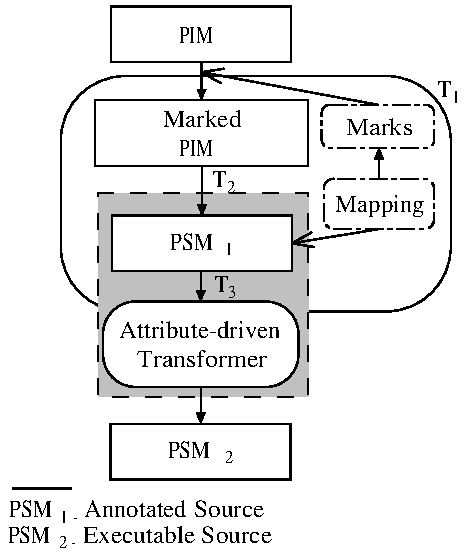
\includegraphics[width=6cm,height=!]{ch03/mda-model2}
	\end{center}
	\caption{MDA Attribute-enabled PIM-to-PSM Transformations}
	\label{fig.gaast-mda-model}
\end{figure}

%Let us now consider how the mapping and interpretation of marked models is different if the target language supports GAAST. 

\begin{figure}[ht]
	\begin{center}
	\begin{minipage}[t]{8cm}
	\begin{scriptsize}
\begin{lstlisting}[numbers=left,language=Java,frame=leftline,showstringspaces=false]{}
[WebService(namespace="www.st.tu-darmstadt.de",
  name="Simple Service")]
class WebService1 {
  [WebServiceMethod(enableSession)]
  string Login(string userName)
  {// TODO: add implementation code here}

  [WebServiceMethod(enableSession,
    transactionOption = TransactionOptions.RequiresNew)]
  ArrayList AcessUserData(string id)
  {// TODO: add implementation code here}
}
\end{lstlisting}
\end{scriptsize}
\end{minipage}	
	\end{center}
	\caption{Mapping to .NET C\#}
	\label{fig.text.2}
\end{figure}

\noindent Discussion:
\begin{enumerate}
\item \textit{Preservation of the PIM} - Converting the HUTN representation of \fig{fig.text.1} to C\# is straightforward. Apart from type and syntax mapping these models are actually equivalent. The transformer for the attribute mapping does not need to access the PIM meta-model. The transformer \texttt{T$_{2}$} can work at the M1 level. This is different from the case of transformers responsible for tag mapping in the marking interfaces approach. Marking interface transformers need details about the meta-model to do the transformation.

With the attribute representation, the model structure is preserved in source code, hence facilitating reverse engineering to the original PIM's architecture. The annotated source can sustain the full design architecture better than pseudo-syntactic marking without having to process method names, and without having to invent many method prefixes or suffixes. 

\item \textit{Complexity of the Programming Model} - The use of annotations simplifies the programming model because marks are still explicit. Having attribute-driven transformation support in the language framework provides the means for processing the language-level PIM. In other words, the part of the transformation concerned with introducing the details of "how" to realize the specified "what" is pushed entirely down to the language level.

The series of commitments in the MDA-based development could start by choosing the target attribute-enabled language. In an attribute-enabled language decorations based on attributes are used directly in code. This would be an alternative design to a graphical UML profile modeling step. Making programs look like designs improves the programming model, given that it decreases the intellectual gap to the domain concepts.

\item \textit{Interpretation of Mappings} -  The interpretation process in the marking interfaces and pseudo-syntactic marking approaches may require third-party tools which can parse and modify the input. An attribute-enabled language serves as a unified framework that does not require any additional third-party tools for parsing the input AST \see{sec:gaast}. 

Having the attribute processing be integral part of the language also simplifies the development of the transformers. Instead of relying on external systems to introduce custom parsing extensions to the language, the language is designed from the beginning to support such kind of transformations. The developer can focus on specific needs of the transformation, e.g., how to integrate transaction management, and not on the \textit{technicalities of the transformation itself}, e.g., on how to parse, access and modify the introduced linguistic abstractions for modeling transaction processing.

Shifting the transformation at the language level helps to achieve tool unification. The target development language is also the transformation tool. The transformation model supported by an attribute-enabled language is the only framework a developer must learn in order to deal with the transformation issues.

\item \textit{Extensibility} - Attribute-based mappings are modular because they directly preserve the PIM architecture and are easy to customize and extend. New issues can be dealt with at any time, by defining appropriate annotations and by introducing corresponding processors to the language framework. The {\tt log} tag example maps directly to a new attribute in this representation, and the mapping does not conflict with any of the other existing attributes. Nevertheless, still care is needed about the order of the transformation during the interpretation \seec{ch04}.
\end{enumerate}

\noindent This section concludes with a short discussion of some of the limitations of an attribute-enabled model-driven development (MDD): 
\begin{itemize}
\item Only the mapping of UML class diagrams with specialized profiles is directly supported by attribute-enabled languages. UML class diagrams map easily to an OO language. The attribute-enabled MDA process was illustrated by the means of the general-purpose object-oriented language C\# \cite{www.dotnet}, whose meta-model maps directly to the class-based web-service model. The transformation process may not be as easy when the UML model elements cannot be directly mapped to the target OO language. Other UML constructs cannot be mapped directly to the source code of a OO language. That is, attribute-enabled languages do not address the complete UML-based modeling of MDA.  %Besides, some profiles contain domain-specific tags that map to well-defined elements of some framework. This has to do with tag interpretation rather than with tag mapping to language constructs. 
%However, if no more specialized domain constructs exist for a given PIM, we could note that given that UML design is OO based \cite{Thomas.Uml.2003}, a general-purpose OO language with GAAST support, makes it easy to map any UML class diagram constructs to source level.

\item
The integrated attribute processing greatly facilitates, but does not automate the implementation of the transformers. While it enables the transformer programmer to concentrate on the semantics of the technical concerns to be integrated rather than be concerned with issues, such as tag extraction, the technical concerns semantics and interactions among transformers still need to be taken care of by the programmer. 
\item
Only the PIM structure is preserved in the language level PSM. Other more fine grained models of the method internals (e.g., using UML actions) will be lost, so only structural reverse engineering is possible. 
\item
The target language must have support for attribute-driven transformations.
\end{itemize}

%Our discussion in this section indicates that we are still away from such vendor supported language technologies that can fully support arbitrary and transparent transformation of source code or meta-data enabled binaries.

\section{Representing Explicit Attributes in {UML}}
\label{sec:problem-statement}

Attributes play an important role in representing custom design-related meta-data \cite{design.attrib,aop.attrib.05,www.aop.metadata,java.compost}, and can be used to expose joinpoints \cite{kiczalesetal.97} \see{ch2:aop}. These usages of attributes require an appropriate representation of attributes at the design time and therefore in UML  \cite{www.uml} diagrams. Several UML extensions using stereotype-like notations have been proposed to deal with specific joinpoints in OO class diagrams \cite{dong02,berner99,aspectj.uml.05}, but none of them deals directly with explicit attributes.

While attributes are similar to MDA MOF \cite{www.mof} tags and UML \cite{www.uml} tagged values or stereotypes, the effect of using attributes explicitly in a programming language, e.g., with Java 1.5 \cite{www.java.meta} annotations and .NET \cite{netattrib} attributes, opens new perspectives to design and program software. UML tagged values and stereotypes model only a subset of design possibilities that can be covered with explicit attributes. This section elaborates on the issue of representing attributes in UML, comparing different possible alternatives that can be used to model different design scenarios. The interest is to find convenient ways to represent explicit attributes in the UML class diagrams.

There are several issues with regard to representing attributes in UML. The first issue comes the used the terminology. In UML (and MOF) the term \textit{attribute} is used to denote class fields: in accordance with OO terminology, a class contains methods and \textit{attributes}. The term is also used with a generic meaning in the UML documentation, synonymously with the term \textit{property}. The term \textit{annotation} does not have any strict meaning in UML. It is used in the UML documentation mainly to denote text notes, i.e., comments. The best fit for a corresponding term for .NET \textit{attributes} and Java \textit{annotations} in UML (and MOF) are \textit{tagged values}. Tagged values are one of the three extensibility mechanisms available in UML (the two others being \textit{constraint} and \textit{stereotype}).

\begin{dinglist}{43}
\item \textit{A tagged value is a keyword-value pair that may be attached to
any kind of model element (including diagram elements as well as semantic
model elements). The keyword is called a tag. Each tag represents a particular
kind of property applicable to one or many kinds of model elements. Both the
tag and the value are encoded as strings. Tagged values are an extensibility
mechanism of UML permitting arbitrary information to be attached to models.}
(UML 1.5 Section 3.17.1 \cite{www.uml})
\end{dinglist}


The UML specification \cite{www.uml} defines in section 3.17, a standard notation for representing tagged values and other custom properties in class diagrams (which describe the static structure of the system). Properties of an element are written after all other data for that element have been specified.

\begin{dinglist}{43}
\item \textit{A property (either a meta-model attribute or a tagged value) is
    displayed as a comma delimited sequence of property specifications all
    inside a pair of braces ( \{ \} ). A property specification has the form
    name = value where name is the name of a property (meta-model attribute or
    arbitrary tag) and value is an arbitrary string that denotes its value. If
    the type of the property is Boolean, then the default value is true if the
    value is omitted.} (UML 1.5 Section 3.17.2 \cite{www.uml})
\end{dinglist}

\noindent There are, however, several problems with the property notation for modeling .NET attributes and Java annotations:

\begin{itemize}
\item Tagged values can only represent a single \textit{\textit{(key, value)}}
  pair. .NET attributes and Java annotations can take more than one
  \textit{(key, value)} parameter. For example, an
  \texttt{[Au\-thor]} attribute may require name and department parameters
  (e.g., \texttt{[Au\-thor(Na\-me=Va\-sian,\-De\-part\-ment\-=TUD)]}). The parameters can
  also be named or positional. Coding this information as a special escaped
  string, in the value part of a tag, makes it error-prone and difficult to
  parse.

\item In .NET, an attribute is a class, whereas in Java it is a special form of
  an interface. That is, a .NET attribute or a Java annotation exists as a
  separate class diagram element in a UML design. By representing an explicit
  attribute as a tagged value, it is impossible to distinguish between a tagged
  value and an attribute by looking at the notation only. A special notation can be used, e.g., an '@' prefix, for those keys that denote attribute names. However, this convention is not supported by default in the UML standard.

\item .NET attributes and Java annotations can take complex type values as
  parameters, such as arrays of constants, or other attributes. The UML tagged
  value notation can be become overloaded with all this information.

\item A .NET attribute and a Java annotation can be used to decorate not only a
  class but also inner class elements, e.g., fields, methods, method parameters, and the return type. The UML property notation can be used in all these cases, but the
  diagrams may become overloaded with information.

\item .NET attributes and Java annotations are used here to
  represent domain-specific abstractions. In this context, attributes serve as a kind of parametrized stereotype, and have the same weight in the design, as a stereotype. The property notation, which is specified after all the other information for an element, does not give any visible clue about the relative weight of the attributes in the design.

\end{itemize}

There is more than one possible alternative for presenting attributes in UML class diagrams\footnote{The issue of presenting
attribute definitions in UML will not be addressed, given that an attribute is similar to a stereotype. As attributes are first-class entities in Java and .NET, attribute definitions can be easily mapped to definitions of a specific
\flqq{}attribute\frqq{} stereotype notation, used to decorate attribute
classes in .NET and annotations interfaces in Java.}, with tagged values being the first candidate. The remainder of this section discusses several alternative UML presentations of explicit attributes, and presents criteria for analyzing the benefits and drawbacks of each notation accordingly.

\subsection{UML Alternatives for Explicit Attributes}
\label{sec:possibilities}

Several UML-based representations could be used to include
explicit attributes in class diagrams. While all these notations use UML
standard mechanisms, they all extend the UML notation in one or more ways.
The intention is to enumerate the most useful possibilities, and analyze the benefits and drawbacks of them. The different UML alternatives are compared based on the following criteria:

\begin{description}

\item[Standard Compatibility:] How good does the notation relate to the overall
  UML standard. Notations that are as near as possible to the UML standard are preferred. Related to standard compatibility is \textit{tool support} (integration in
  existing tools): Existing UML tools  \cite{case.tools} can easier support minor extensions that fit into the overall UML designs, rather than major changes.

\item[Visibility:] How good does the notation emphasize the importance of
  attributes in a UML design. Notations that emphasize the
  attribute semantics are preferred. Explicit attributes are often an
  important part of the design, and their relative weight should be properly
  expressed in the UML class diagrams.

\item[Clarity:] How clear or verbose the notation is. The less
  verbose notations are preferred. Verbose notations can be difficult to manage when they are used to decorate internal class elements, e.g., method parameters. Verbose notations could also result in cluttering of the UML diagram with too many elements.

\item[Usability:] How easy it is to use or reuse a given notation, e.g., being able to have a single definition of an attribute in a diagram and then reuse it via associations. Reuse is preferred, as it means less maintenance efforts. Related to reuse is \textit{ease of use}, that is how convenient a notation is to use, in order to model an explicit attribute.

\item [Representation Structure:] The preferred notations sustain a more structured attribute representation, compared to those that simply represent attributes as 
  strings. Structured notations are less error prone and easier to manipulate
  automatically.

\end{description}

\begin{figure}[ht]
	\centering
	\begin{minipage}[b]{8.5cm}
	\begin{center}	
		\begin{scriptsize}
\begin{lstlisting}[numbers=left,language=Java,frame=leftline,showstringspaces=false]{}
@Author(
    name="Vasian Cepa",
    name="Sven Kloppenburg")
@DAO
public class Account {
    
    @PrimaryKey
    private string accountID;
    
    ...

    @Transactional(kind=Required)
    public void credit(float amount)  { ... }

    @Transactional(kind=Required)
    public void debit(float amount)  { ... }
        
    public float getBalance() { ... }

    ...
}
\end{lstlisting}
		\end{scriptsize}
	\end{center}
	\caption{Attribute Annotation Example}
	\label{fig:app.example}
\end{minipage}	
\end{figure}

\noindent The main possible alternatives for presentation of
explicit attributes in the UML class diagrams are discussed next. The example of \fig{fig:app.example}, modified from \cite{www.aop.metadata}, will be used to illustrate the various alternatives.  The example shows how a bank account class can be modeled by utilizing several Java 1.5 annotations. There are two class level attributes: \texttt{[Author]} and \texttt{[DAO]}\footnote{Data Access Object.}, that denote the authors of the class, respectively, that the class needs to be processed in order to enable data persistence. Inside the \texttt{Account} class, there is a string field \texttt{accountID}, which is decorated with a \texttt{[PrimaryKey]} attribute as part of the data persistence functionality. This field will be used to identify the \texttt{Account} class records, when they are persisted in the database. Several of the class methods are decorated with a \texttt{[Transactional]} attribute, to denote that they must always be called as part of a transaction. Of course, not all code entities have attribute annotations, as illustrated by the \texttt{getBalance()} method. The UML examples below use a \textit{tilde} ('$\sim$') sign to separate multiples values in a UML property string value notation as needed, and an \textit{at} ('$@$') sign to decorate attribute name strings. Possible alternatives are separated with \textit{semicolons} ('$;$').

\begin{description}

\begin{figure}[ht]
		\centering
		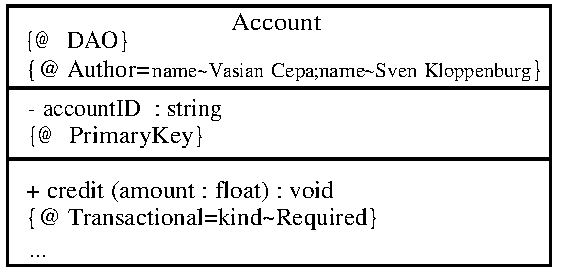
\includegraphics[width=7cm,height=!]{append1/properties}
	\caption{Attributes as UML Properties}
	\label{fig:tagged.values}
\end{figure}

\item[UML properties, tagged values:] This is the first UML representation possibility that comes to mind for attributes. The details and problems of this case were discussed in \sr{sec:problem-statement} to motivate the need to explore other notations. In order to represent the explicit attributes, the property notation needs to be extended (a) with a special notation, e.g., '@', used before the attribute names, and (b) to enable the string values to have an inner structure, in order to represent the key--value pairs of the attribute arguments. The extended notation is illustrated in \fig{fig:tagged.values}.
  
  The modification of the UML standard is minimal, and could be easily supported by
  any existing tool that supports UML properties and tagged values. The
  notation can become verbose, when too many attributes and attribute
  parameters are used in a class, or other inner elements, e.g., method parameters. The attribute annotations applied to an element cannot be reused. The annotation has to be copied and pasted around. This notation is not very structured, especially the value part of the string, and can be error prone.

\begin{figure}[ht]
		\centering
		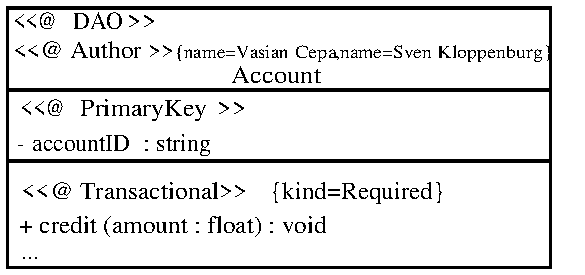
\includegraphics[width=7cm,height=!]{append1/stereotype}
	\caption{Attributes as UML Stereotypes}
	\label{fig:stereotype}
\end{figure}

\item[Stereotypes:] An alternative to the UML properties and tagged
  values for representing attributes is to use the stereotype notation, as in \fig{fig:stereotype} \cite{berner99}. In this case, the name of the attribute is used as a stereotype to decorate
  the UML elements. To distinguish a stereotype that serves as an attribute from other
  stereotypes, a special '@' character can be added before the name. An
  extension is needed to include the attribute parameter list with the help of a
  special notation, for example, by using an extended UML property notation as
  part of the stereotype instance name.

This notation is slightly better than the extended UML properties notation. Using the stereotype notation for the attribute name, rather than the usual property notation, shows explicitly the weight of the attribute in the design. It could also be relatively easily supported by the existing UML CASE tools. The notation is not very structured, especially the parameters part. 

\begin{figure}[ht]
		\centering
		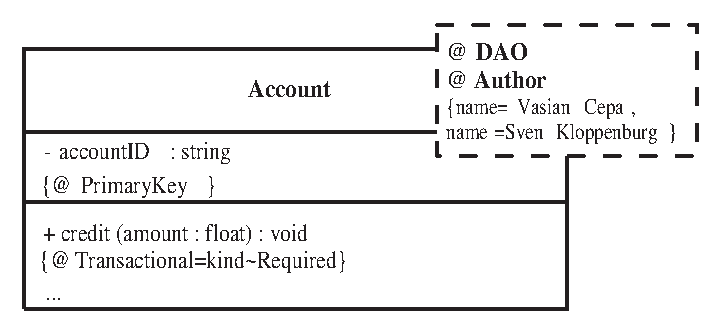
\includegraphics[width=9cm,height=!]{append1/template}
	\caption{Attributes as UML Template Parameters}
	\label{fig:template}
\end{figure}

\item[Template-like notation:] The C++ template argument notation,
  supported by the UML, can also be used to represent explicit attribute instances (\fig{fig:template}). This
  notation places even more weight to the role of an attribute, and could be
  useful in cases where attributes are very important in the design. The template notation can also be useful when the space inside the class-name box is scarce and there is a large number of attributes with a lot of parameters that need to be specified.
 
 The template
  notation will not work well with explicit attributes that annotate the inner
  elements of a class, e.g., object attributes, methods and method
  parameters. A variant of the template notation places in the template box the
  values of attributes for all member elements of a class, inside separate sub-boxes.
  This variation may require some kind of mapping between the
  attributes and the existing members. The notation could become verbose for
  the overloaded methods, where the method name is reused and cannot be used alone as a
  mapping tag. The template notation (without sub-boxes) could be easily supported by
  UML CASE tools. A benefit of the template notation is that all class-level attributes are located within a single easily visible place.

\begin{figure}[ht]
		\centering
		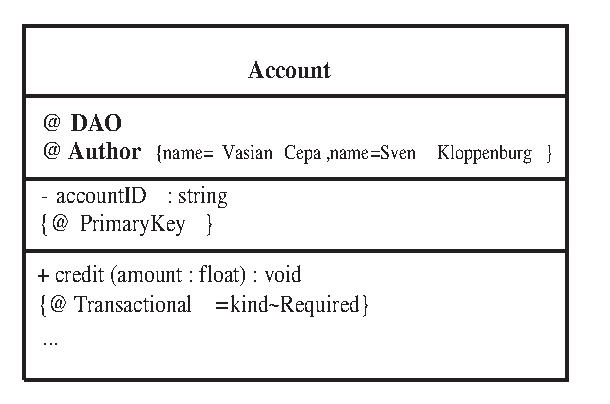
\includegraphics[width=7cm,height=!]{append1/box}
	\caption{Attributes as Extra Class Sub-Box}
	\label{fig:partition}
\end{figure}


\item[Class partitions:] Explicit attributes could form a separate sub-box inside the class notation, similar to
  fields and operations, as in \fig{fig:partition}.
  The sub-box notation could be seen as a natural way to extend the class
  definition semantics. Another variation is to have an explicit optional
  attribute sub-box for each kind of element in a class, such as fields and operations. The attribute sub-box is a stand-alone unit within the class model, and the notation has the same benefits and drawbacks of the template-like notation. The separate sub-box can be used in the UML tools that do not support the template notation.
  
\begin{figure}[ht]
		\centering
		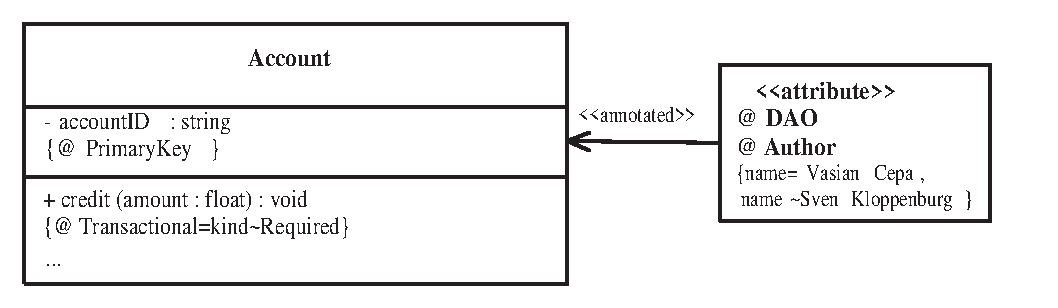
\includegraphics[width=12cm,height=!]{append1/class}
	\caption{Attributes as Separate UML Class}
	\label{fig:class}
\end{figure}

\item[Separate classes:] Explicit attributes can be also represented by a separate class-like notation with an \flqq{}attribute\frqq{} stereotype associated with the class, as illustrated in \fig{fig:class}. There are two variations of this representation: (a) one similar to the template notion, containing all the attribute notations for all
  elements of a class, (b) a separate class for the attributes of each inner element, associated directly with the annotated element.
  
  In the case of sub-elements, e.g., methods, the class notation may require that the association lines intersect the class boundaries and link directly to the methods or other inner elements, a feature that may not be supported by the standard conformant UML tools. The class notation is more reusable and more structured that the previous possibilities.

\begin{figure}[ht]
		\centering
		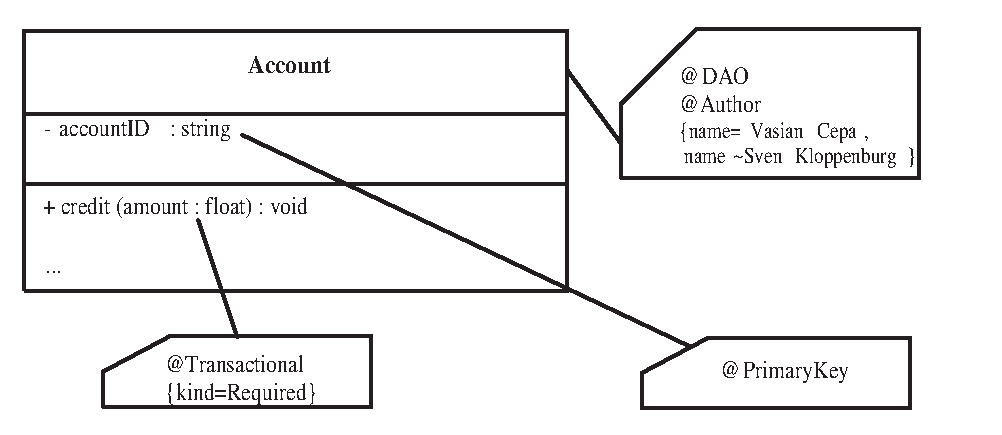
\includegraphics[width=12cm,height=!]{append1/comment}
	\caption{Attributes as Comment Boxes}
	\label{fig:comment}
\end{figure}


\item[UML comments:] Comments allow arbitrary text labels to be associated with every
  UML element. Comments can be used to model explicit attributes
  as shown in \fig{fig:comment}. Comments are unstructured, so there may be a need to place some implicit structure in the text string. For example, an '@' character can be used before a name to denote that it is an attribute.
  The selected implicit notation can be tool and language specific. The comment notation lacks the inner structure, and it may be difficult to distinguish between attribute comments and other types of comments in a diagram. Apart of this, the notation is as reusable and flexible as the separate class notation.

\end{description}

\subsection{Discussion of the UML Alternatives}

Table~\ref{tab:AttributePresentationInUML} summaries the above discussion, evaluating the alternative UML notations discussed above against the criteria given in \sr{sec:possibilities}. Plus signs indicate that a criteria is better supported. Minus signs indicate less conformance to a given criteria.

\begin{table}[ht]
	\begin{center}
		\begin{tabular}{|l||c|c|c|c|c|}
		\rowcolor[gray]{.7}
\hline
 Presentation &   Standard & Visibility &  Clarity &      Usability &  Structure \\

\hline
Properties &      + +      &      - -      &      - -      &      -      &      -      \\
\hline
Stereotype &       + +     &       +     &      -      &      -      &       -     \\
\hline
 Templates &       +     &       +     &       -     &       -     &      +      \\
\hline
 Partition &        -    &       +     &       -     &        -    &       +     \\
\hline
Separate Class &     +       &     + +       &     +       &     + +       &     + +       \\
\hline
   Comment &       +     &      +      &     -       &      + +      &      - -      \\
\hline
		\end{tabular}
	\end{center}

	\caption{Summary of Various Explicit Attribute Presentations in UML}
	\label{tab:AttributePresentationInUML}
\end{table}

As indicated by the Table~\ref{tab:AttributePresentationInUML}, no representation is better suited than all the other with regard to all criteria. The separate class notation seems to fulfill most of the requirements, however, it may have difficulties to represent the annotation of the inner class elements.

Table~\ref{tab:AttributePresentationInUML} shows that some notations are better suited that the others is some direction. This is a consequence of the various scenarios that could be covered with explicit attributes in a UML model. Depending on the
relative weight of the attributes in the design, their parameters, and the density of the attribute usage in a class, or in the class inner elements, different notations may be useful in different situations. 
%
For example, it could be chosen to represent attributes that serve as marking interfaces \cite{design.attrib} by stereotypes, given that this expresses their importance. When many explicit attributes are used to drive generation and they are repeated over classes, a separate class notation makes more sense. For fine grained notations, e.g., method annotations, or method parameter annotations, an extended variation of UML properties is less verbose and hence better suited. More than one notation could also be combined in the same diagram, as was the case with some of the UML examples in \sr{sec:possibilities}.

Finally, based on the Table~\ref{tab:AttributePresentationInUML}, it can be concluded
that the stereotype and separate class notations are the two most usable notations that should be considered as a first choice to model the explicit attributes in UML class diagrams. In several cases, some notation based on the UML properties is needed to augment the other representations. Several of the analyzed extensions may not be supported by all UML CASE tools.

\section{Languages with Generalized and Annotated Abstract Syntax Trees}
\label{sec:gaast}

This section discusses language technology organized around annotated Abstract Syntax Tree (AST)-like representations of program structure, used to support attribute-based DSA in product-lines. This section also discuses the impact of such technology on the processing of attribute annotated code entities.

%Generalized and Annotated Abstract Syntax Trees (GAAST) are a lightweight language extension mechanism relying on: (i) tagging program code with attributes and (ii) implementing transformations based on reflective-like Abstract Syntax Tree (AST) API-s. Two features are important for this purpose: (a) support for explicit meta-representation of programs as an AST-like structure accessible in a programmatic way before and beyond the compilation, and (b) support for user-defined annotations of program elements.

\subsection{Attribute Language Support Example: .NET Languages}
\label{c3.sec.dnet}

To illustrate the relation between annotations and AST-like representations of the program structure, this section considers .NET framework \cite{www.dotnet}, as a representative of systems with explicit support for tag interpretation, by means of access to source, or binary representations of programs.
%
.NET follows a hybrid approach with respect to attributes. It distinguishes between \emph{predefined} and \emph{custom} attributes. Predefined attributes are used by various library API-s that come bundled with the .NET platform. For example, \texttt{[Sy\-stem.Dia\-gno\-stics.Con\-ditional\-Attribute]} is used by the compiler to include methods conditionally in the compiled version. In contrast to the predefined attributes, custom attributes do not have a meaning to the compiler. The code to interpret custom attributes has to be implemented explicitly by the developer that introduces the attributes to model domain-specific concepts.

In .NET, an attribute is a normal class derived from a predefined \texttt{Sy\-stem.Attri\-bu\-te} class. Attributes are part of the type system and can also be marked with other attributes. The interpretation code can be placed inside the attribute class itself. When a larger context needs to be processed, in order to interpret the attributes, the interpretation code could also be placed in a separate module. 

\begin{figure}[ht]
	\begin{center}
		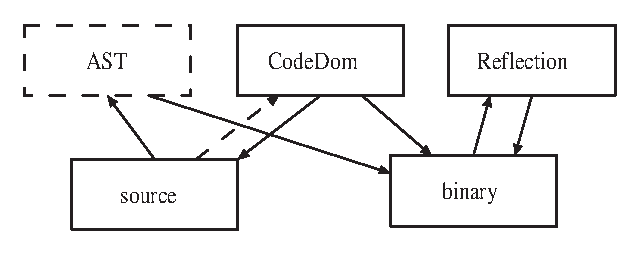
\includegraphics[width=7cm,height=!]{ch03/existing}
	\end{center}
	\caption{.NET AST-Like Program Representations}
	\label{fig.existing}
\end{figure}

\fig{fig.existing} shows a high-level view of the .NET API-s that support access to different AST-like representations of a program. There are by default two main ways how .NET API-s can be used to process attributes:

\begin{itemize}
\item \textit{Source code manipulation.} The .NET \texttt{Sy\-stem.\-CodeDom} API \cite{cdom}  supports source-level AST-like representation and manipulation of a program. An implementation of this API can be used to build an AST, either manually, or from the source code of a program (by means of \texttt{ICode\-Parser}\footnote{The current .NET framework language specific providers do not implement \texttt{ICode\-Parser}. For this reason, the connection from source to \texttt{CodeDom} box in \fig{fig.existing} is drawn as a dashed line. A free third-party implementation for C\# is \textit{CS CODEDOM Parser} \cite{cs.codedom.parser}.}). Next, the constructed AST-like representation can be transformed and the result AST is saved (back) as source (by means of \texttt{ICo\-deGene\-rator}), or it is directly compiled to a binary file (by means of \texttt{ICo\-deCompi\-ler}\footnote{ \texttt{Sy\-stem.Code\-Dom.Compi\-ler} interfaces (and helper classes) must be implemented by a \texttt{Code\-Dom} compiler provider.}).

\item \textit{Run-time manipulation.} The .NET {\tt Sy\-stem.Re\-fle\-ction} API can be used to (a) introspect a binary for its structural elements and the attributes they are decorated with, as well as in the reverse direction, (b) to create executable modules (assemblies). For the latter purpose the {\tt Sy\-stem.\-Refle\-ction.Emit} API can be used (in combination with the Reflection API) to generate the method internals. While the Reflection API deals with creating the program structure elements, e.g., classes and methods, the {\tt Emit} API deals with Intermediate Language (IL) opcodes used inside methods. The {\tt Emit} API works only in one direction. It can generate new assemblies, but cannot access or modify the IL representation of the existing ones.
\end{itemize}

\begin{figure}[ht]
	\begin{center}
		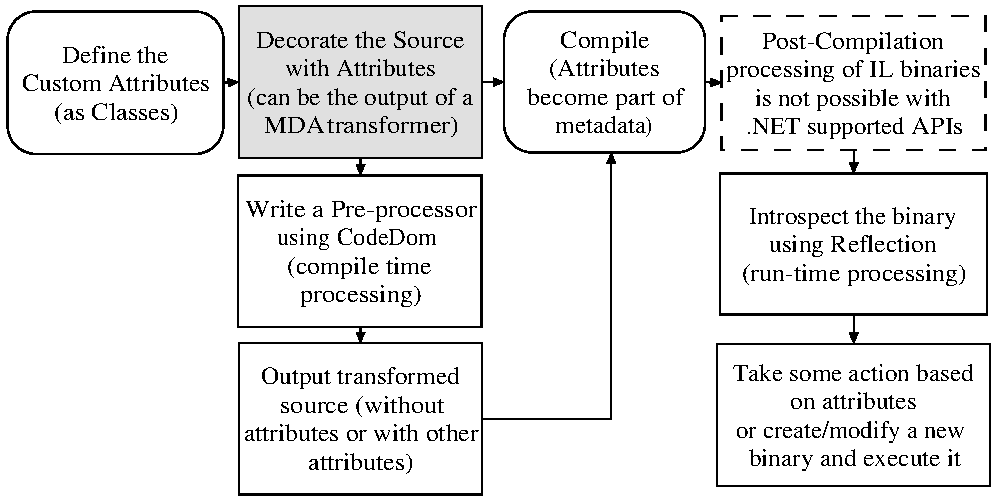
\includegraphics[width=12cm,height=!]{ch03/net-attribute-processing}
	\end{center}
	\caption{Processing Attributes in .NET}
	\label{fig.processing}
\end{figure}

.NET API-s provide an infrastructure for creating and accessing AST-like representations of a program beyond the parsing stage of the compiler. \fig{fig.processing} shows how this infrastructure can be used to interpret attributes in .NET. The first step to utilize the custom attributes in .NET consists in defining new attribute classes (when needed), and using them to decorate the code. The exact actions to be performed next depend on the semantics associated with the used attributes. In a next step, the source-level AST, obtained via  \texttt{CodeDom}, is used to modify the source code. Alternatively, the code is compiled and the attributes become part of IL binary meta-data. The IL meta-data are accessed later-on at run-time, via the {\tt Reflection} API, and are processed to undertake user-defined actions. Post-compilation manipulation of existing IL binaries is not directly supported by the .NET API-s.

\subsection{GAAST-Based Language Technology}
\label{sec.gaast}

\fig{fig.existing} contains also a dashed box named {\tt AST}, which is not discussed so far. This box represents the AST that is internally constructed by the compiler, during the compilation process of the source code. In .NET, this AST is not available to the end-programmers. The {\tt AST} box is shown in \fig{fig.existing} to emphasize the similarity between the different .NET AST-like representations of the program (aimed at supporting program transformations), and the source AST built by the compiler. The .NET CodeDom, or Reflection ASTs, and the compiler AST represent the same information at various levels of detail.

\begin{figure}[ht]
	\begin{center}
		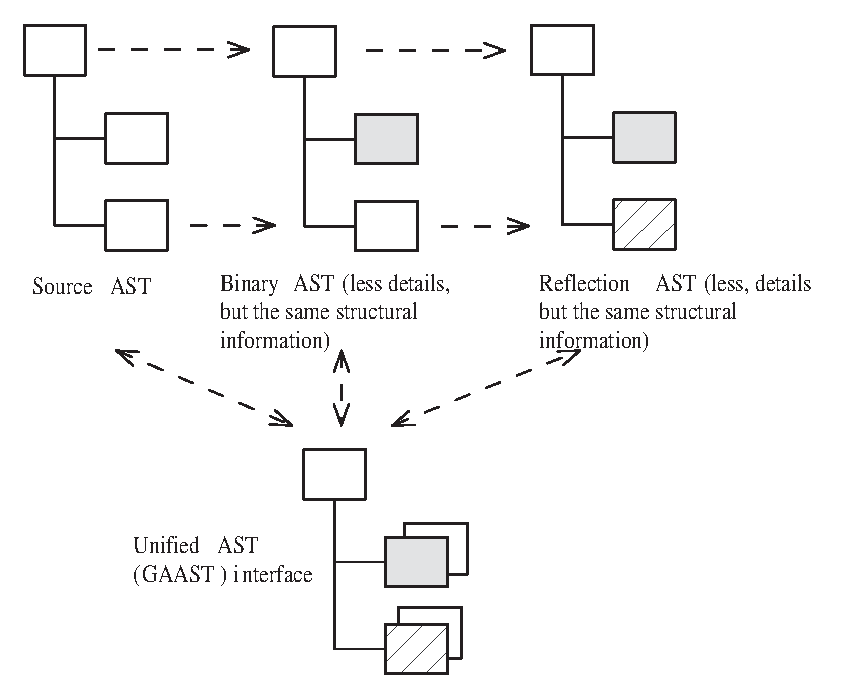
\includegraphics[width=10cm,height=!]{ch03/gaast}
	\end{center}
	\caption{Unified AST Representation}
	\label{fig.gaast}
\end{figure}

This similarity suggests the idea of having a single common AST-like representation of a program, that would be used by the compiler, as well as, by other attribute-driven transformers in a programming language with annotation support. Such an AST API, that generalizes over different ASTs of the same program and supports annotations, will be called a \textit{Generalized and Annotated AST} (GAAST) API. There are several aspects of a GAAST API that need to be especially discussed:

\begin{itemize}
\item \textit{Modeling AST differences.} As illustrated in \fig{fig.gaast}, there could be differences in the information found in different representations of the program. Some nodes present at source code are not preserved in the binary representation, or could be presented by different element nodes (gray filled in \fig{fig.gaast}). A common example is deploying a prefix or suffix increment / decrement operator. The GAAST API is intended to support attribute-driven transformation for implementing DSA constructs. The source code AST representation is too fine grained attribute-driven transformers. The GAAST API can unify the structural information and leave out the other details. Some nodes can be present in the interface, but a given implementation of GAAST may choose not fill all nodes with valid, or fully parsed information \see{dnet.gaast}. This situation is represented by different fillings of (possibly empty) nodes in the unified AST, at the bottom of the \fig{fig.gaast}.

\begin{figure}[ht]
	\begin{center}
		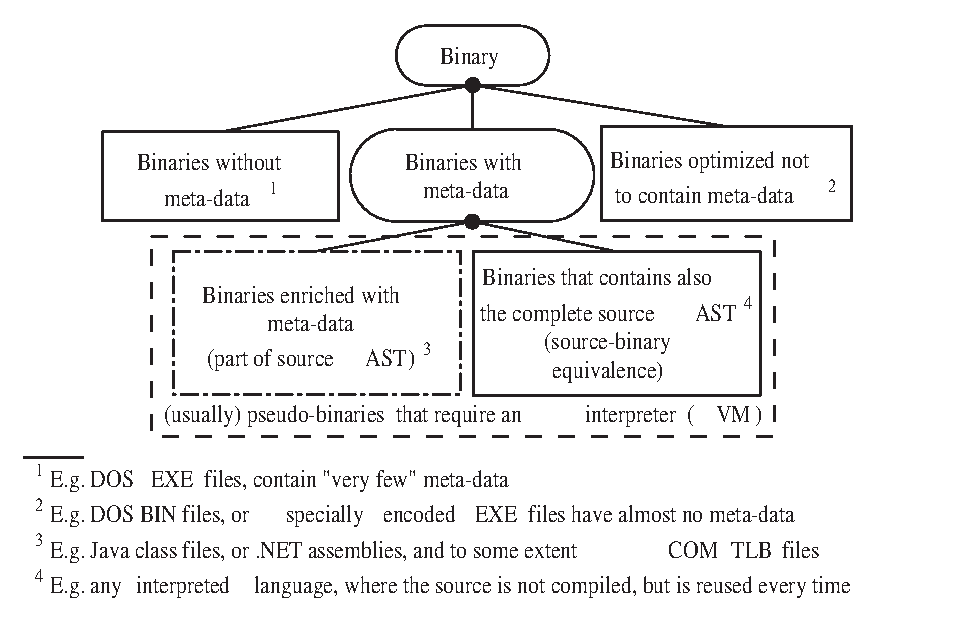
\includegraphics[width=12cm,height=!]{ch03/metadata}
	\end{center}
	\caption{GAAST Relation to Meta-data}
	\label{fig.meta-data}
\end{figure}

\item \textit{Matching the language features.} GAAST reflects the features and the dynamicity of the underlying language system. The source code manipulation enables static transformations. Many language systems support only static transformations, because they do not save the AST information as part of their \textit{pseudo-binaries}. \fig{fig.meta-data} shows a rough classification of what is understood by binaries in this section. The meta-data, as shown in \fig{fig.meta-data}, is a way to explicitly save part of the AST obtained from the source code along with the compiled code. The amount of the AST information saved as part of meta-data determines the level of reflection that is possible at run-time in a given language system. The reflective transformations require languages that have enough meta-data to support run-time introspection, represented by the dash-dotted box in \fig{fig.meta-data}.

Languages, such as Java or .NET, save almost all structural information found in source code as part of the binary meta-data. These language technologies usually do not preserve a one-to-one map of those parts of the AST that represent control-flow (behavior), e.g. \textit{for} loops. Obtaining such fine-grained control structures requires some reverse engineering. 
%
In languages that support meta-data as part of their binaries, the GAAST API could support also static binary manipulation. In reflective languages, GAAST may support either static or dynamic transformations, depending on the language run-time support for reflection.

\item \textit{GAAST as a Language Workbench.} Extending a programming language to support a GAAST-like API is relatively easily, when only specific features of GAAST are needed. For example, any static meta-programming framework can be used as a GAAST-like API for static source code transformations, as long as the framework preserves and enables access to the AST attributes. This makes a GAAST-like API an attractive lightweight language expression to support attribute-based transformations in mobile product-lines \seec{ch05}.

\begin{figure}[ht]
	\begin{center}
		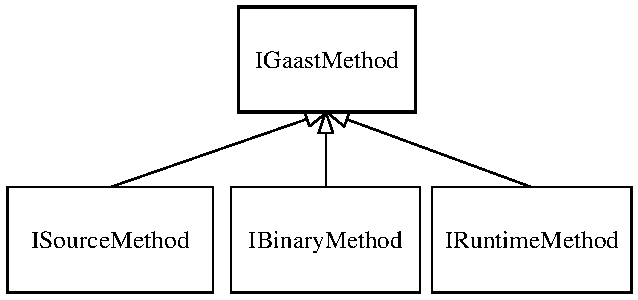
\includegraphics[width=6cm,height=!]{ch03/native}
	\end{center}
	\caption{GAAST Language Information Organization}
	\label{fig:native}
\end{figure}

A more advanced view is to consider GAAST as part of the language system itself. That is, to make the unified GAAST API a central part of a language framework supported by the language vendor. The other API-s, such as the compiler AST, {\tt Reflection}, or {\tt CodeDom}-like API-s, could be organized around the common GAAST interface, as illustrated by the method interface example in \fig{fig:native}.

A language with GAAST support for attribute-driven transformations can be seen as a language workbench \cite{lang.workbench} to sustain attribute-based DSA. The GAAST API serves as a \textit{contract interface} between the language workbench features, provided by the language vendor, and third-party attribute transformers. It becomes the responsibility of the language vendor to maintain the contract interface as the language evolves. Several languages, e.g., .NET or Java, are already moving into this direction.

In a GAAST-enabled language, the attribute transformers are immune to most changes in the language workbench (e.g., several syntax changes). This is difficult to warranty with third-party implementations that need to be separately maintained, adding accidental complexity to the product-line. In a GAAST-enabled language, the transformer developers would not need to reinvent helper API-s and tools that are covered by the GAAST API. Transformers could reuse third-party modules build on top of the central GAAST and better leverage rapid prototyping. The language platform vendors would also profit from the unified GAAST API, since by unifying several API-s, the total cost of the language platform is decreased and the language system becomes also more attractive to the programmers.

\end{itemize}

\noindent GAAST addresses only the parsing issues related to source or meta-data enriched binaries. Attribute-driven transformation based on GAAST-like API-s will be fully discussed in \kr{ch04}. Specialized abstractions could be built on the top of the GAAST API that would facilitate building transformers. There are two concepts that can be used in combination to implement generic abstractions over a GAAST infrastructure:

\begin{itemize}
\item GAAST can be enhanced with declarative query capabilities. An example of query capabilities is {\tt JPath} API for Java developed as part of {\tt EXTRACT} \cite{extract} compiler system. JPath defines a set of operations for selecting nodes from a Java AST, borrowing the idea from W3C XPath \cite{url.xpath} standard for XML \cite{skonnardetal.01}. Another example of query support directly embedded in the langauge, is the query expression pattern of .NET C\# 3.0 language specification \cite{csh30}, based on the LINQ \cite{linq} project.

\item Support for declarative specification of transformations. This is similar to the ideas put forward by OMG MOF Query / Views / Transformations (QVT) proposals \cite{mof.qvt}. In terms of QVT, JPath is a query and view language. QVT also exposes means to define transformations. Transformers take a view as a parameter and map it to another view. This is similar to graph rewriting techniques \cite{term.rewrite,mens.99,gme.graphs}, but provides a more declarative way to define graph transformations. At the time of this writing a final MOF QVT standard is not yet available. 
\end{itemize}

\subsection{Implementing GAAST on Top of .NET}
\label{dnet.gaast}
Having stressed the importance of supporting GAAST as a central part of the language technology, \fig{fig.third} shows how a third-party prototype GAAST API can be implemented on top of the existing .NET API-s.

\begin{figure}[ht]
	\begin{center}
		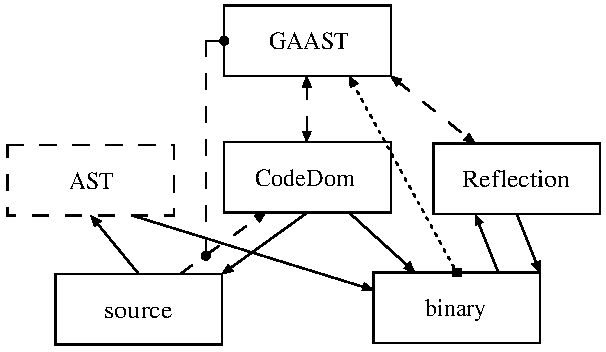
\includegraphics[width=7cm,height=!]{ch03/third}
	\end{center}
	\caption{Implementing GAAST on Top of .NET}
	\label{fig.third}
\end{figure}

The dotted arrow, from the {\tt binary} box to the {\tt GAAST} box, represents the required custom code to expose the method internals of IL binaries through the GAAST API, which is currently not supported by the .NET Re\-fle\-ction API. The dashed line connecting {\tt source} and {\tt Code\-Dom} boxes represents the implementation of the {\tt ICo\-de\-Par\-ser} interface, which is also currently missing in .NET.

Unfortunately, a third-party API cannot directly reuse the AST built by the language compiler(s), and does not have access to the .NET Common Language Runtime (CLR) information, unless a supported interface to expose this functionality is provided. The lack of this interface renders the implementation and maintenance of a third-party framework difficult, especially in face of the evolution of the .NET framework.

\begin{figure}[ht]
	\centering
	\begin{minipage}[b]{8.5cm}
	\begin{center}	
\begin{scriptsize}
		\begin{lstlisting}[numbers=left,language=Java,frame=leftline]{}
namespace System.Reflection {

 public class MethodInfo : MethodBase {
	
  public Type ReturnType
  { get{ ... } }
		
  public object[] GetCustomAttributes(bool inherit)
  { ... }
  ...
 }
}
		\end{lstlisting}
		\end{scriptsize}
	\end{center}
	\caption{Reflection API Method Representation}
	\label{c3:netref}
\end{minipage}	
\end{figure}

As an example, consider \fig{c3:netref}, that shows how the \textit{methods} information is modeled by the .NET Reflection API. The Reflection API enables the introspection of a method to get information about it, e.g., to find the custom attributes that have been used to annotate the method and its return type. When using the Reflection API, the types returned by the methods, e.g., \textit{Re\-turn\-Ty\-pe}, are properly resolved, and the system has access to the full loaded assemblies, which makes it possible to return, for example, the attributes inherited from a base class method (the \texttt{bool inherit} option of the \texttt{Get\-Cu\-stom\-Attri\-bu\-tes} method).

\begin{figure}[ht]
	\centering
	\begin{minipage}[b]{8.5cm}
	\begin{center}	
\begin{scriptsize}
		\begin{lstlisting}[numbers=left,language=Java,frame=leftline]{}
namescpace System.CodeDom {

 public class CodeMemberMethod : CodeTypeMember {

  public CodeTypeReference ReturnType
  { get{ ... } set{ ... } }
		
  public CodeAttributeDeclarationCollection CustomAttributes
  { get{ ... } set{ ... } }

  public CodeCommentStatementCollection Comments
  { get{ ... } }
  ...
 }
}
		\end{lstlisting}
		\end{scriptsize}
	\end{center}
	\caption{CodeDom API Method Representation}
	\label{c3:netdom}
\end{minipage}	
\end{figure}

\fig{c3:netdom} shows how the same information is modeled by the .NET Code\-Dom API. The first difference concerns the returned types. For example, the type returned by the \texttt{Re\-turn\-Ty\-pe} is not a fully-resolved \texttt{Ty\-pe}, but a \texttt{Co\-de\-Type\-Re\-fe\-rence}, which could be either an unresolved user defined type, or a resolved system type. Another difference is that the \texttt{Cu\-stom\-Attri\-butes} method cannot resolve hierarchy information. Information for additional nodes, e.g., code comments, is also present, which makes no sense for binary files. The most profound difference is the capability to modify the information, as can be noted by the \texttt{set} version of the supported properties in \fig{c3:netdom}. The Reflection API provides read-only access to the method information.

\begin{figure}[ht]
	\centering
	\begin{minipage}[b]{8.5cm}
	\begin{center}	
\begin{scriptsize}
		\begin{lstlisting}[numbers=left,language=Java,frame=leftline]{}
namescpace Gaast {
	
 public interface Method : Member {

  public Type[] ReturnType
  { get{ ... } set{ ... } }
		
  public CustomAttribute[] CustomAttributes
  { get{ ... } set{ ... } }

  public Comment[] Comments
  { get{ ... } set{ ... } }
  ...
 }
}
		\end{lstlisting}
		\end{scriptsize}
	\end{center}
	\caption{GAAST API Method Representation}
	\label{c3:netgaast}
\end{minipage}	
\end{figure}

A possible common GAAST-like interface is shown in \fig{c3:netgaast}. The GAAST interface enables writing the same structural transformations, despite the underlying program representation. When no complete native language support for GAAST exists, as is the case with .NET, a third-party GAAST API, based only on the CodeDom and the Reflection API, could only offer a set of uniform interfaces to access the common information. To initialize the GAAST interface, a factory pattern \cite{dpatterns} can be used, similarly to the way .NET CodeDom supports different .NET languages. The factory can support either source, or run-time representations. A trade-off to model the AST differences could be to ignore representation specific information and throw a missing implementation exception on \texttt{set} methods, when only a read-only view is supported.% The situation can be partially improved if other third-party frameworks for processing .NET binaries can be used and through custom access to the .NET CLR data, for example using the .NET profiler.

In practice, unless GAAST languages become available, a third-party GAAST API implementation can be reasonably limited, by implementing only those aspects of the GAAST technology that are needed by a specific transformation system. As the focus is on DSA support with attributes, only the static aspects of GAAST API are explored in attribute-driven transformations. Various aspects the GAAST technology for supporting static and run-time attribute transformations are investigated in the upcoming chapters. A custom GAAST-like API build for Java 2 Micro Edition MIDP \cite{www.midp}, which uses JavaDoc \cite{jw-pollac} tags to emulate annotations, is described in \kr{ch:mobcon}. The Tango transformation engine, introduced in \kr{ch04}, supports a GAAST API for static transformations based on a common XML representation of the program structure, enabling either source or binary transformations, if they can be expressed in the common XML format. The Attribute Dependency Checker tool of \kr{ch04} uses the run-time aspect of GAAST, based on the .NET Reflection API, to automatically enforce system-wide attribute dependencies.

\section{Comparison to other DSL Approaches}
\label{sec.related.dsl}

Attributes could be used to emulate DSA constructs in mobile product-lines. There are two aspects how this particular usage of attributes is related to other generic systems that can be utilized to implement DSA:
\begin{enumerate}[1.]
\item Attributes can be seen as a convenient way to extend the grammar of the language. Attribute-based DSA only cover a subset of possible EDSL approaches, and are limited in the grammar changes they can introduce. Attribute languages enable implicit grammar extensions. \Sr{sec.ext.grammars} discusses this aspect of attributes languages, as languages with implicitly extensible grammars. 
\item When combined with AST manipulation, e.g., via a GAAST-like API, attributes enable meta-programming techniques. \Sr{sec.meta.prog} discusses the relation of GAAST with other meta-programming systems, intended for easing the DSL implementation. The discussion of the relation between the attribute-driven meta-transformations and other transformation techniques will be postponed until \kr{ch04}, after the attribute transformations for mobile product-lines are explained.
\end{enumerate}

There are several approaches \cite{deursenetal.00,kamin.98,cardelli94extensible,batory98jts,stratego.01,hudak98modular,java.jse,java.epp,java.maya,java.openJava} that have been proposed to reduce DSL and EDSL implementation costs. These approaches address (i) grammar extensions and (ii) parsing costs, as well as, the (iii) interpretation costs. As it will be argued in the remainder of this section, with these approaches, the start-up costs remain still higher than those of other variability mechanisms used for product-lines, e.g., OO frameworks \see{sec:ooframeworks}. These approaches also often introduce heavy external dependencies on third-party tools \see{sec:var.dsa}.

GAAST-enabled languages remove entirely the costs related to (i) grammar extensions and (ii) parsing, for the category of EDSL extensions that can be modeled as attributes \see{sec.ext.grammars}. The advantage of using attributes directly in a GAAST-enabled language is that the programmer does not need to deal directly with the grammar modification \cite{Taha.1997}. Attribute declarations and usage are supported by the system and do not require changes to the compiler. In a GAAST-enabled language, explicit attributes \cite{java.explicit.programming,hedin.97} add new semantics to the existing nonterminals of the grammar. The core grammar does not change, only its semantics change selectively. The change of the semantic applies only to the annotated elements. This enables supporting more than one set of attribute-based DSA at the same time, in a given GAAST language. \Kr{ch04} explains techniques that address the (iii) interpretation issues of the attribute-based DSA.

For an analogy that illustrates the relation between the attribute-based DSA approach and the other open language supported meta-approaches \cite{cardelli94extensible,batory98jts,java.jse,java.epp,java.maya,java.openJava} with regard to (i) grammar extensions and (ii) parsing, consider meta-modeling with MDA MOF \cite{mda.frankel,www.mof} and UML \cite{www.uml}. To extend the elements used in a MOF model, its meta-model needs to be extended. The meta-model extension requires knowledge about the meta-model and how to modify it. An alternative solution is supported in UML by the means of profiles. With profiles, a UML meta-model can be extended without explicitly modifying the meta-model definition. UML profiles achieve such modifications by restricting the types of possible meta-model extensions to stereotypes, typed values, and constraints. These three generic mechanisms enable changing the semantics of existing meta-model elements selectively. Furthermore, UML profiles enable to define these extensions at the same abstraction level as the model, making the meta-model manipulation implicit. 

Attribute-based DSAs, unlike the other approaches, make the manipulation of the language meta-model implicit. Explicit attributes can be logically mapped, more or less, to UML parameterized stereotypes \see{sec:problem-statement}. Similarly to MDA MOF, the attribute-based DSA introduces the possibility to manipulate and extend the language grammar meta-layer, a feature that is missing in most widely used programming languages. Attributes are a central part of a GAAST-enabled language, forming a low-cost language workbench \cite{lang.workbench} to support DSA. 

\subsection{GAAST Languages and Extensible Grammars}
\label{sec.ext.grammars}
Programing languages need often to be extended with various constructs, which are made part of their syntax. Extensible compilers \cite{extensible.compilers} support language extensions as part of their original design. Extensible compilers require the modification of the parser, the modification of the semantic analyzer, and other back-end passes (e.g., optimization and generation \cite{muchnick.97}) \cite{extensible.compilers}.

AST annotations are traditionally used during contextual analysis and code generation in compilers \cite{java.compilers.book,morr.02}. This book promotes the use of the AST annotations explicitly \cite{java.explicit.programming} in the source code. The GAAST languages, described here, can be seen as an extensible front-end of a compiler.
%
A grammar that support explicit attributes (tags) will be called a \textit{tagged grammar (TG)}, a term that does not conflict with any other existing grammar terms \cite{Parsing.Techniques.90}. The tagged grammar term is used to refer to the grammars that support GAAST languages. A compiler that supports a TG-based language has an extensible front-end. 

Any language grammar can be extended. There are approaches, e.g., extensible grammars (EG) \cite{cardelli94extensible} that structure the changes applied to a grammar, into a series of basic modification operations. EG reduce the costs of introducing and maintaining incremental grammar modifications. An EG is a grammar augmented with \textit{constructor} functions for creating productions, and three (meta) grammar operations:
\begin{enumerate}[1.]
\item \textit{addition} - introduces a new production in the grammar, by expressing it in the terms of grammar constructors,
\item \textit{deletion} - removes a production from the grammar, by making the grammar more restrictive,
\item \textit{update via replacement} - updates an existing grammar rule, by replacing it with the new definition. 
\end{enumerate} 

The expressiveness of an EG grammar depends on the rules found in the \textit{core grammar}. Phobos \cite{java.phobos} is a system for Java based on the ideas of extensible grammars \cite{cardelli94extensible}, that structures the grammar changes as module (grammar) inheritance. The focus of this section is in TG expressiveness for supporting EDSL, as compared to more full-fledged EG. There are two ways how a TG can be utilized to support attribute-based DSA:

\begin{enumerate}[a.]
\item \textit{As an extensible grammar} - TG are restricted in the ways they can modify the core grammar. A TG cannot introduce arbitrary changes. The expressiveness of a TG is limited as compared to an EG. In formal terms, a tag can be seen as a nonterminal symbol $\tau \in T$, with $T$ being the set of the allowed tag strings\footnote{The $T$ set is infinite, but only a finite number of strings are used from it in a program.}. A tag that accepts parameters can be expressed as tags without parameters \see{ch03:sec:attrib.param}. A tag enables adding only productions of form $N_{new} \rightarrow \tau N$ to the grammar, where $N_{new}$ is a new nonterminal and $N$ is a nonterminal that exists in the original grammar. An EG supports adding productions of form $N_{new} \rightarrow \alpha_{1} N \alpha_{2}$, where $\alpha_{1}, \alpha_{2}$ are either nonterminals or terminals. This means that a TG can generate less string forms than an EG. 

%Indeed, for a context-free grammar \cite{Parsing.Techniques.90}, the expansion of $\alpha_{1}$ and $\alpha_{1} N$ does not depend on the rule context. The expansion of $\alpha_{1}$ can be treated as a new tag $\tau_{1}$ and used to replace $\alpha_{1}$  in the expansion of $\alpha_{1} N$. The complete expansion of the $\tau_{1} N$ can also be treated as a new tag $\tau_{2}$. This leads to a production of form $N_{new} \rightarrow \tau_{2} \alpha_{2}$, which falls in the form of a TG production. The (right) expansion of $\alpha_{2}$ can be done recursively in the same manner. If the grammar has no loops, an expansion of form $N_{k}\tau_{k}$ may appear, which obviously cannot be expressed as a new rule in a TG grammar.

\item \textit{As a transformation system} - In this view, the annotation capabilities of TG are used to mark transformation points (explicit hooks \cite{java.compost}) over the elements generated by the core grammar. The modifications of the core grammar are external to the grammar itself. The production $N_{new} \rightarrow \tau N$ is interpreted as a transformation function $\tau: N \rightarrow \tau(N)$. Tag parameters can also be modeled as a parameter vector $\pi$, so the generic tag transformation function becomes $\tau: N \rightarrow \tau(\pi, N)$ \see{attrib.trans}. The function $\tau$ maps the domain $N$ into a co-domain $N_{new} \in TG$\footnote{$N_{new}$ may map into several productions in the core TG.}. This way, while remaining in TG, any transcendental transformation semantics can be applied via $\tau$. The expressiveness of the semantics, as in the case of EG-s in \cite{cardelli94extensible}, depends on the core TG (without tags).

\end{enumerate}

It is the arbitrary transformation view of a TG that is of interest in practice. The grammar production context is removed in a TG, from the grammar to the transformation system. When combined with a transformation system, a TG can be used to express the same semantics as an EG with minimal changes. Any computationally-complete general-purpose programming language can be used as a candidate for a core TG. In practice the implementation of transformation $\tau$ could be easier, if the language supports at least directly some of the language mechanisms intend to be used by $\tau$. For example, attribute transformations applied to classes are easier to support in an OO language, where the classes are natively supported, rather than in a non-OO language. 

GAAST languages can be also used to support other program transformations apart of attribute-based DSA. The GAAST API (and its implementation) could help with technical concerns related to AST processing, so the effort to obtain the AST for the source code is not repeated in custom transformers. The GAAST does not replace other approaches for building EDSL-s. GAAST is rather an intermediate transformation tool that can be used in the intermediate transformation phases of other tools that need to do AST processing.

\subsection{Meta-Programming Approaches}
\label{sec.meta.prog}

The approaches discussed in this section \cite{java.openJava,batory98jts,www.self,java.jse,java.epp,java.maya} ease one or more aspects of DSL, or EDSL implementation. They, however, do not make the grammar manipulation as implicit as GAAST languages do \see{sec.related.dsl}. Some of these approaches can also be used to implement attribute-driven transformers. The reverse is also true. GAAST-enabled languages remove the need for many of these third-party approaches. 

\noindent \textbf{Meta-programming systems} are language systems that contain support to process and modify the elements of their own meta-model. There are two categories of meta-programming systems:

\begin{itemize}
\item \textit{Static} meta-programming systems, e.g., LISP \cite{lisp}, or OpenJava \cite{java.openJava} are very similar to the GAAST concept. They provide access to the meta-model of a program and enable source-to-source manipulation. Some static meta-programming systems, e.g., OpenJava \cite{java.openJava} or Jak \cite{batory98jts}, support adding new types of terminals not found in the core grammar, and enable translating these new constructs to the core grammar entities. 

\item \textit{Reflective} meta-programming systems, e.g., Smalltalk \cite{smalltalk}, Self \cite{www.self}, or ECMA\-Script\footnote{The JavaScript OO model is quite similar to Self.} \cite{ECMAScript}, enable programs to query and, depending on the system, to modify their own meta-information. Forms of reflection can be found in all modern general-purpose programming languages, e.g., .NET and Java. Reflection in these systems is limited to querying information only. Other systems, e.g., Self \cite{www.self}, can also modify their types and type hierarchies at run-time.

\end{itemize}

The only way to extend a GAAST language are attributes. This means that generic meta-constructors are not required in a GAAST language. The meta-model is only implicitly extended. Only when the attributes are processed the meta-model manipulation becomes explicit in a GAAST language. A GAAST API reflects the properties of the language. If a language supports reflective meta-programming, a GAAST API for that language could be made available. In languages, such as .NET, the GAAST API enables only static meta-programming\footnote{Reflection in .NET can be combined with a GAAST API, but full reflective meta-programming capabilities are not supported.}.

The remainder of this section presents two examples of static meta-systems in more detail. The selected examples were chosen because (a) they are implemented as generic language extensions, introducing external third-party dependencies in the systems that rely on them, and (b) they are not strict meta-systems, but contain also features that support EDSL implementation.

\noindent \textbf{Jakarta Tools Suite (JTS)} \cite{batory98jts} facilitates the DSL creation by offering a set of related tools that address the complete process of implementing DSL. The JTS tools include:
\begin{itemize}

\item \textit{Bali} is parser generator used to support parsing custom DSL grammars, similar to JavaCC \cite{javacc} or ANTLR \cite{antlr}.  Based on a given grammar specification, Bali generates a lexer, a parser, and a hierarchy of Java classes to represent the parsed AST.

\item  \textit{Jak} \textit{"is an open, extensible superset of Java"} that extends Java with \textit{"support for meta-programming"}, and \textit{"enables Java programs to write other Java programs"} \cite{batory98jts}. Jak provides access the parsed AST and enables manipulating it using Java-like code. Jak can be used alone, or as a back-end for Bali. Jak can parse at run-time uncomplete code snippets (called surface syntax trees) and can validate them with regard to types and symbols in the context of another AST. Jak can also support generation scoping by limiting the identifiers scope to sets of related code fragments (environments). Jak provides also several predefined AST traversal operations similar to Stratego \cite{stratego.01}.

\item A  mix-in \cite{bracha90mixinbased} \textit{way} to compose language extensions and any set of mix-in features, known also as \textit{GenVoca} \cite{genvoca.94} generators. GenVoca is a scalable model for composition of component-based software that generalizes the concept of mix-ins\footnote{In the sense that every possible software composition is treated as feature mix-in.}.
\end{itemize}

JTS tools have been successfully used to implement complete DSL that support product-lines \cite{dsl-pl.2000}. Dealing with grammar evolution is still explicit in JTS approaches. Jak supports source-to-source transformations and is similar to the .NET CodeDom API, but has also generic constructors to create new types of statements or expressions. 

Being third-party extensions, Bali and Jak need to be explicitly maintained as the Java language evolves. For example, the evolution of Java from version 1.4 to 1.5 was not followed by the JTS. To overcome these issues, in \sr{sec.gaast} it was required that GAAST be part of the programming language technology, as it is the trend with .NET (CodeDom, Reflection API-s) and to some extent with Java 1.5\footnote{An unsupported API similar to CodeDom is distributed from Sun with Java 1.5.}.

In order to benefit from GenVoca compositions, clear decomposition of the domain features must be available. However, many software problems do not have a clear feature-based decomposition structure \cite{foa-aop.04}, so that they cannot be easily composed as chains of independent features\footnote{A feature-based decomposition structure is typical for abstract data collections and some mathematical libraries.}, reducing the applicability of GenVoca compositions for organizing the AST transformations.

GAAST-enabled languages address only attribute transformations. This means that GAAST-enabled languages are a special case of a meta-programming system. In a GAAST language, a tool, such as Bali, is not needed, whereas support for the AST manipulation is assumed to be part of the language, removing also the need for Jak-like tools.

\noindent \textbf{Macro systems} \cite{java.jse,java.epp,java.maya} can be used to support DSA constructs. Macros are used in languages, such as C, to extend the language with declarative constructs. Macros are processed by a preprocessor, usually by replacing the definition with the macro code. The systems mentioned above support \textit{syntactically rich} macros, where the macro definition can access the AST of the code at the point of the macro application, and modify its own behavior based on the invocation context. This enables implementing more powerful macros, which are not possible in languages, such as C. Syntactically rich macros can be used to implement DSA constructs, and help to address grammar and parsing issues.

While the mentioned macro systems do not have support for attributes, such support could be easily added. The macro systems could be used for static source-to-source attribute-driven transformations, similarly to the .NET CodeDom API. Syntactically rich macros are usually implemented as third-party language extensions, and have the same problems with regard to the language evolution as Jak \cite{batory98jts}.

\textbf{Summarizing}, GAAST languages have a more limited scope than all other extensible meta-programming systems. Attributes support only a very specific set of EDSL, and not all possible EDSL can be expressed as explicit attributes. What makes attributes attractive is that, they are either part of a GAAST language, or require a minimum one-time effort to be added. Attribute-based DSA can also be processed with any meta-programming tool that exists for a given host language, requiring minimum new investment in a product-line. Extending the meta-model of a language with custom attribute-based DSA does not require any knowledge about the grammar manipulation and parsing. When attribute processing is part of the language (GAAST is supported), there are no external dependencies of a product-line to third-party DSL implementation frameworks. Attributes expose a uniform programming model, free the user from having to learn new syntax, and have minimal education and training costs compared to the other approaches. 

Attributes have the lowest start-up costs for supporting DSA in a product-line. While attribute-driven transformations should still be applied, most of the time they require a simple mapping from the attribute-based DSA, to the component libraries implementing the common domain functionality. Attribute-driven transformations add only a very small burden with respect to the implementation cost of component libraries, and can be used as a mechanism of choice for iterative development of a product-line.

\subsection{AOP and DSA}
\label{sec.aop.dsa}

Aspect-Oriented Programming (AOP) \cite{kiczalesetal.97} was mentioned in \sr{sec:var.dsa} as an example of generic language systems that can be used to support DSL. AOP was technically discussed in \sr{ch2:aop}. This section compares AOP and DSA along two dimensions: (a) AOP as a way to implement DSA, and (b) AOP as a replacement for DSA.

\noindent \textbf{AOP as a way to implement DSA.} \Sr{sec:aop-inv} discussed that AOP engines can be used as generic invasive systems to implement various transformations including the interpretation of the DSA constructs. There are, however, several liabilities, that prevent AOP engines from being used to implement arbitrary DSA constructs:

\begin{itemize}
\item \textit{Hardwired joinpoint / pointcut models.} A distinction can be made between AspectJ \cite{Laddad.aop, www.aspectjt}, and more recent AOP systems. AspectJ is a declarative meta-pro\-gramm\-ing system that hides the meta-model manipulation from the end programmer. AspectJ has a hardwired joinpoint / pointcut model that, as explained in \sr{sec:aop-inv}, covers many generic meta-programing scenarios, but not all. Adding support for different, extensible joinpoint and customizable pointcut models is possible \cite{www.abc,josh.04}, but could remove some of the benefits of stated in \sr{sec:aop-inv}, e.g., static checking, invested efforts on IDE support, and declarativeness. It also blurs the distinction between AOP systems and other kinds of meta-programming, or open compiler systems. %More run-time support \cite{prose,java.steamloom} will likey blur the distinction with active OO databases, whereas support for more than one meta-model \cite{XIRC} is likely to converge to MDA MOF \cite{www.mof} style transformations.

\item \textit{Limited vertical\footnote{Horizontal transformations are used in this section to mean transformations that work within the same meta-model. Vertical transformations work across different meta-models \cite{sf.04} \see{ch2:aop}.} transformations.} A software system is often programmed using more than one language. For example, Java, SQL, various script and declarative languages based, for example, on XML, or visual languages can be used together. DSA can introduce abstractions that crosscut more than one single language technology. DSA enrich the meta-model of a language, and can isolate alien parts of a system to make them look native in any technology \cite{riel.96}. For example, Hibernate \cite{hibernate} provides Java abstractions around object / relational JDBC \cite{www.jdbc} databases. When using Hibernate, the relation schema of a given database becomes accessible from Java, as normal Java classes. This means that, the AspectJ engine can also be used to manipulate them, which was not possible without Hibernate generated wrappers. Introducing technology wrappers only to support AOP techniques can be costly.

AOP engines have limited support for vertical transformations that cross-cut more than one meta-model. Aspect engines that support more than one language meta-model, need to work upon some common meta-model of all supported system models. In terms of MDA MOF, such a common joinpoint meta-model will be a M2 level model \see{c2.vm}. M2 level models are very generic, to be useful for very specific transformations, which makes them not as suitable as language specialized aspect engines. For example, \fig{fig:xml-mda} show schematically the inner workings of an XML-based AOP approach \cite{XIRC} for cross-model manipulation. This approach works at the same logical level as MOF M2 level (the meta-model of XML itself is M2 level with regard to data modeled in XML)\footnote{The reverse is also true. The MOF can be equivalently mapped to the XML meta-model. An example is XMI \cite{mda.frankel}.}. The approach supports only the query view of the execution graph \see{ch2:aop}, because xQuery \cite{www.xQuery} requires access to the total XML DOM tree. The M2 level compatibility found in \cite{XIRC} should not be confused with language families, such as the .NET language family \cite{Weave.NET}, that share the same meta-model, but map it to different concrete syntaxes.

\begin{figure}[ht]
	\begin{center}
		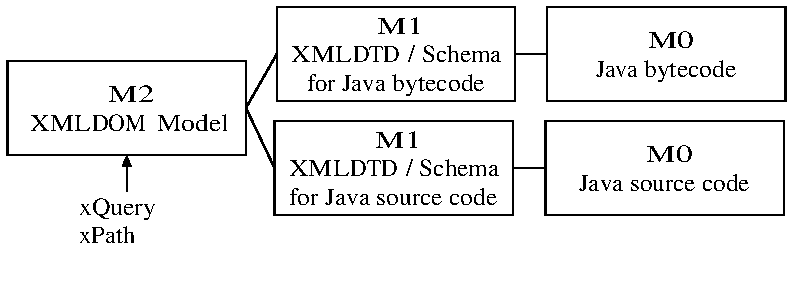
\includegraphics[width=8cm,height=!]{ch03/xml}
	\end{center}
	\caption{The XML MDA Levels}
	\label{fig:xml-mda}
\end{figure}

Working at the meta-model level unifies many specific issues that are usually important to be ignored. For the example of \fig{fig:xml-mda}, the XML queries will be more useful if they refer to the information from the M1 level models. Elements of the M1 models, e.g., language specific features, can be explored in a joinpoint model to allow more semantically rich pointcuts. This is not possible when working with the M2 level elements. However, queries specialized for one M1-level model cannot be used for another M1-level model.

%\item \textit{Arbitrary extension points.} Generic AOP engines help with declarative specification of joinpoints and with implicit meta-programming changes. The advice code itself \see{ch2:aop} can be structured with any usual OO mechanism. The freedom of implementation is good for a generic transformation framework. However, \sr{sec:ooframeworks} stressed the need for well-defined extension points in product-lines, which is difficult to enforce over the aspect implementations in generic AOP engines\footnote{In theory, adding another meta-level to the AOP programming model that is, having aspects over the aspects, can help to enforce well-defined extension points. The programming model of this meta-meta-system will be difficult to be understood by humans.}.

\end{itemize}

\noindent \textbf{AOP as a replacement for DSA.} While any generic transformation system can be used to implement DSA, no generic transformation system can replace DSA. DSA promote an explicit programming style and enrich the meta-model of a language. The programmers select explicitly the context where DSA constructs will be used. AspectJ and AOP replace the explicit programming style with selection of points of interest, enabling in theory more automation. DSA preserve the domain architecture in the code. Whereas AOP, when used as a replacement for DSA, hides the domain architecture, which makes it not suitable for emulating the DSA semantics. While AOP techniques cannot replace DSA, neither can DSA replace AOP techniques. They complement each-other and could be used together in a system. AOP engines can be used to apply AOP-style modularization in a system, working over the DSA constructs.

The consequences of AOP-style modularization are outside the scope of this work. Technically speaking, matching AOP pointcuts is a mechanical process \see{sec:aop-intro}. While pointcuts are declarative, the points of interest need to be specified often as complex composed pointcuts. The shadows of complex composed pointcuts cannot be directly imagined by humans for large systems. This means, that there could be points that are matched when they should not, and vice-versa. Investment in IDE support for AspectJ can help with this regard for a particular AOP system. Other systems \cite{alpha.05} explore less fragile pointcut models to deal with evolution of source code artifacts. While this is an area of active research, the mechanical pointcut matching is still far from replacing the human search and could result in unpredictable transformation side-effects. Attributes can be used as a workaround to express complex pointcuts, that are too complicated to be expressed otherwise. AOP techniques will not be explored any more in this book. The focus will be on the DSA support with attributes, and it will be left up to the user to decide the most appropriate programming model, on a case by case basis.

\section{Proper Usage of Explicit Attributes}
\label{sec.attribute.usage}

Attributes are easy to introduce and can carry any semantics. This can lead to \textit{abuse} of AEP, when attributes are utilized to represent semantics that can be represented better with other language means. This section discusses the proper usage of explicit attributes, giving several examples of inappropriate practices.

\subsection{When to Annotate?}

Every program element can be decorated with explicit attributes. There are natural ways to define the semantics of abstract software models in all programming languages. The OO language abstractions are usually easier to use than the explicit attributes, and are also better statically checked by the language compiler with no additional effort on the part of the developer. The following principle summarizes the first guideline for properly using explicit attributes.  

\begin{principle}
\label{pri:tagUsage}
Explicit attributes should be used to decorate an entity, when there is no simpler natural representation of the intended semantics, supported by the hosting language.
\end{principle}

\noindent The term \textit{natural} is intuitive \cite{mozart.04}, and so is the usage of tags to denote extended semantics. Everything, that can be done with attributes, can also be done without them in a Turing complete \cite{automata.2001} language. According to the principle~\ref{pri:tagUsage}, attributes help to reduce the accidental complexity, and to make the abstractions easier to introduce and implement. Several alternatives how to use explicit annotations are possible and have already been used, however, not all of them follow the principle~\ref{pri:tagUsage}, as illustrated by the examples below:

\begin{itemize}
\item Attributes can be used to decorate any element if it is allowed by the language grammar. In an OO language, decorating a 'Car' object with a 'color' tag can be more naturally implemented with a field attribute of the class 'Car'. In .NET C\# \cite{www.dotnet} decorating a structure with a custom attribute 'class' to denote OO class semantics makes no sense, given that the available 'class' keyword is the natural choice.

\item Explicit attributes can be used to augment programming languages with new constructs in a convenient way. Decorating a structure with a custom attribute 'class' makes sense in the ANSI C language to denote a class. Attributes enable customization  of a language without changing its grammar. For example, using marking interfaces to translate marked UML class diagrams to source code results in a large number of interface derivations to represent multiple tag values, as was shown in \sr{attributes}. It is more natural to deploy an attribute-based approach.

\item Non-consistent designs also exist. For example, a serializable object can be distinguished at the run-time\footnote{For example, to be able to serialize an object instance to be sent over the network during remoting \cite{dnet.remoting}.} if its class implements a required serializable marking interface. It adds nothing semantically to use both an explicit attribute and a marking interface \cite{design.attrib} to decorate a class.
%
However, implementing the serialization in .NET requires both an interface and an attribute, favoring the attribute for generation, and using the interface for the required serialization methods that need to be implemented\footnote{In practice, this design makes sometimes sense, because it reuses as much of the existing language abstractions as possible, rather than relying only on generation techniques based on attributes.}.

\item Explicit attributes can be used to represent the declared model of an application, by defining \textit{explicit hooks} \cite{java.compost} where code can be inserted. What \textit{declared model} means is a relative concept. A class definition, marked with an additional 'enterprise' attribute, contains more semantics than a class definition without this attribute. However, as shown in \fig{fig:convert}, the implicit program model can be made automatically explicit with attributes, without adding any semantics to the design.

\begin{figure}[ht]
\begin{center}
\begin{minipage}[t]{8cm}
		\begin{scriptsize}
		\begin{lstlisting}[numbers=left,language=Java,frame=leftline]{}
class WebService1 { public void Method1() {...} }
 
// goes to:

[Class(Name="WebService1")]
class WebService1 {
    [Method(Name="Method1", Modifiers="Public", ReturnType="void")]
    public void Method1() {...}
}
\end{lstlisting}
		\end{scriptsize}
		\end{minipage}
	\end{center}
	\caption{Converting the Implicit Model to an Explicit Model}
	\label{fig:convert}
\end{figure}

This means that the mere existence of explicit attributes does not show the existence of a meaningful declared model, upon which one can reason about the application's components.

\item Attribute decorations are local. It makes few sense to use local attributes for introducing global system-wide functionality. For example, local attribute decorations are used in \cite{bodden.04} to check global properties at run-time. Placing the same code in a separate module, would be more suitable and would cut in half the implementation effort. If the checked conditions are local in scope, existing Java 1.5 assertion statements would make more sense.

\end{itemize}

\subsection{What can be Annotated?}
\label{when.annotate}

It may seem that in an attribute enabled language everything can be decorated. However, the \textit{identifiable elements} of a program are different, in different representations. Sometimes the structural elements of a program, e.g., namespaces and classes, are invisible when source code is compiled to a binary file. It should be properly clarified what could be decorated, and how long this decoration is about to last. The following principle summarizes the right targets that be annotated:

\begin{principle}
\label{pri:tagTarget}
Only entities that exist and can be manipulated in a given context, can be decorated with attributes.
\end{principle}

\noindent The generic term \textit{'entity'} was used on purpose. An 'entity' is whatever can be distinguished in some way from the rest of the environment. It can be a class, a method, an object, a thread, a 'for' loop etc. 
The 'entities' have to exist in the context where the annotation is applied, and when it is interpreted. A 'for' loop exists in the AST of the source code and can be decorated. But the 'for' loop does not exist in the same form in the binary output of a compiler. Therefore the 'for' loop attributes cannot be preserved in that binary representation. Another example, is the possibility to annotate object instantiation in the source code level, because the line and the syntax are known. At run-time, an object can be decorated immediately after it is created, but the instantiation process itself cannot be decorated. 

As a consequence of this principle, there are three different contexts, where explicit annotations can be applied:

\begin{itemize}
\item \textit{Source-code level} - Attributes can decorate structural elements (e.g., classes and methods) and behavioral elements (e.g., loops and conditionals). Attributes can be processed by a preprocessor tool, or by the front-end phase of a compiler. Attributes can also be preserved for later use in the binary meta-data. However, many source-code level attributes that support code generation (e.g., used to introduce new class fields) should be processed partially or completely before or during compilation \seec{ch04}. Other source-code level attributes that decorate elements, that will not exist any more as separated entities in a binary (e.g., \textit{for} loops), need to be fully processed before compilation.

The attribute specifications in both .NET\cite{www.dotnet} and Java \cite{www.java.meta} state that attributes do not change the semantics of the code they decorate. This means that a component decorated with attributes should be able to be compiled and used even though the attributes are not processed. In practice there are many exceptions to this rule. Components decorated with attributes usually cannot be used, unless the attributes are properly processed, given that the attributes change the semantics of the component, or the semantics of the context \cite{.net.context.attrib} it lives in\footnote{That is, the attributes are an integral part of the overall semantics of a component.}. In other cases, attributes can be used to introduce fields or methods that are used by the rest of the code. Such scenarios arise often when attributes are used to drive code generation. In these cases, the component cannot compile without processing first the attributes.

\item \textit{Binary level} - Not all languages offer this possibility. In real binaries, the structural source code information is not present. The source-level equivalent entities are either not preserved, or are blurred in undeterminable ways by various semantically-equivalent compiler optimizations \cite{muchnick.97}. Meta-data enriched pseudo-binaries found in languages, such as Java and .NET, save the structural information of the source code AST inside the binary \see{sec.gaast}. In such languages, the annotation of the structural elements is preserved during compilation and can be accessed after the compilation, or at the run-time, by using reflective introspection. For example, Soot \cite{soot.00} can statically explore and modify the Java bytecode format.

\item \textit{Run-time level} - New entities exist at run-time that are not found in the source code or binaries. For example, in the source code level there are class definitions and object instantiations instructions. The real objects exists only at run-time. The same holds true for threads and virtual methods.
%
The need for attributes at run-time can be easy emulated with additional object attributes\footnote{The \textit{'Variable State'} pattern \cite{gamma.eclipse.04} can be used for specific objects or a lookup (hash) table for all objects indexed by the object.}, and will not be explored any more in this book\footnote{Using reflection at run-time to manipulate attributes is a case of binary-level attributes, and not of the run-time level attributes.}.
\end{itemize}

These contexts differ in the amount of static or dynamic information that is available. Different language technologies also differ in the amount of the information that is made available in each context. Java annotations \cite{www.java.meta} make these contexts explicit. A Java annotation can have source, binary, or virtual machine lifetime. For example, the \texttt{@Re\-ten\-tion(\-Re\-ten\-tion\-Po\-li\-cy.\-RUN\-TI\-ME)} meta-attribute denotes that a given attribute should be preserved during the execution by the Java virtual machine.




\cendsection{Chapter Summary}
\label{ch03sum}

Attributes are a lightweight language extension used to introduce custom domain-specific abstractions (DSA). Attribute-based DSA support a declarative programming model for product-line development. Attribute families organize the attributes in nested name spaces corresponding to the domain assets. Attributes can be used to drive DSA transformation\footnote{Source to source, source to binary, binary to binary and / or binary to source.} in the language technologies that support them. An attribute enabled language provides the possibility to decorate and access the decorated AST in various (equivalent) representations of the source code.

Attribute enabled languages support more directly model-driven development (MDD) compared to other language technologies used to map UML class diagrams, such as, marking interfaces, or pseudo-syntactic marking. Attribute programming helps to preserve architectural decisions in the source code. Unlike interface based mapping and pseudo-syntactic mapping, attribute mapping closely resembles the original MDA models and provides for better extensibility and a less complex programming model for the targeted OO languages. The mapping process is also simpler. Attribute enabled languages help to close the gap between thinking in terms of models, and source code.

Attributes enable new ways to design the code. UML tags and stereotypes can model only a subset of attribute design possibilities. While mapping UML tags and stereotypes to attributes is straightforward, the reverse process is not directly supported in every case by UML. Several UML notations were investigated, that can be used to model different attribute-based scenarios. 

GAAST enabled languages make it easier to extend a general-purpose OO language with domain-specific constructs. GAAST languages offer a single uniform mechanism to introduce custom extension. GAAST languages  serve as a convenient alternative to extensible compilers, for implementing attribute-based DSA. GAAST languages do not require changing and maintaining the front-end tools of the compiler. If the GAAST technology is supported by the language vendor, it becomes easy to introduce AEP in an existing project, and to maintain attribute-transformers in the long term. Languages, such as .NET and Java 1.5, already offer a lot of support for GAAST-like transformations.

Attributes should be used carefully to enhance or replace software abstractions that are already available in a language. Adding attributes is easily, however, just using attributes \textit{per se} adds no semantic value to the source code model. The set of the used attributes and their scope validity should be carefully selected, based on the domain concerns. Attributes can be preserved in various representations of the source code or the binary, if the language technology allows it. Depending on the interpretation scope, attributes can be used at (pre) compile time, after compilation, or at run-time.

%ch04

\chapter{Building Modular Attribute-Driven Transformers}
\label{ch:tango}
\label{ch04}
\mquote{All animals are equal, but some animals are more equal than the others.}{G. Orwell, Animal Farm, 1946}
\mquote{All transformations are equal, but some transformations are more equal than the others.}{(Variation)}

\noindent This chapter\footnote{This chapter shares content with references \cite{cepa.tango.ICSR8,cepa.mezini.gpce.04,cepa.mezini.hicss38,cepa.2006}.} addresses the implementation of modular attribute-driven transformers by exploring features that are specific to DSA modeling of mobile product-lines with attributes. The developed technology can be used, as well, with other attribute-driven transformations.

Using explicit attributes at the programming language level has recently been attracting a lot of attention with technologies, such as .NET attributes \cite{design.attrib} and Java 1.5 annotations \cite{www.java.attrib.04}, and also with specialized tools, such as xDoclet \cite{www.xDoclet}\footnote{xDoclet does not work at the language level.}, used with EJB \cite{www.ejb}. However, there are currently no systematic ways for transforming attribute-driven product-line specific constructs. This often results in implementations which are not very modular and hence difficult to reuse.

\begin{figure}[ht]
%	\begin{center}
	  \xymatrix{
	  	*+[F]{\txt{Attribute Transformation \\\Sr{sec.attribute.trans}}} \ar[r] \ar[d] \ar[dr]& *+[F]{\txt{Layering Transformation Strategy  \\\Sr{sec.tango.layers}}}  \\  	
	*+[F]{\txt{Automating Transformation Concerns \\\Sr{ch04:sec:dep}}} \ar[r] \ar[d]  	 & *+[F]{\txt{Related Work \\\Sr{sec.c4.related}}} \\  	
	  *+[F]{\txt{Attribute Dependency Checker Tool \\\Sr{sec:adc}}} 	  &   \\	  	
	  }
%	\end{center}
%	\caption{Chapter Overview}
%	\label{fig:contents}
\end{figure}

\Sr{sec.attribute.trans} shows how the AST could be modeled to ease attributes transformation in mobile product-lines. The addressed domain is explored to introduce a horizontal modularization of transformers. The OO language model of MIDP \cite{www.midp-ota} is used in \sr{sec.tango.layers} to layer the transformation strategy.

Automating attribute transformation concerns using meta-attributes is addressed in \sr{ch04:sec:dep}. A specialized tool, called ADC, for checking attribute dependencies based on meta-attribute decorations, is presented in \sr{sec:adc}.

Several generative and graph transformation techniques could be used to implement attribute-driven transformers. Related transformation and automation approaches for the techniques developed in \srs{sec.attribute.trans}{ch04:sec:dep} are discussed in \sr{sec.c4.related}. 

\section{Attribute-Driven Transformations}
\label{sec.attribute.trans}

The concepts discussed in this section have been implemented as part of an attribute-driven transformation framework, called \textbf{Tango}\footnote{The name \textit{Tango} was coined in the following way: tag $\rightarrow$ tag-go $\rightarrow$ taggo $\rightarrow$ tango.}. The Tango framework is designed to quickly add attribute-based domain-specific constructs to existing object-oriented (OO) languages, by reusing the existing language functionality. Tango has evolved as a generalization of the work on the \textbf{MobCon}\footnote{Mobile Container.} Transformation Engine (MTE), to support mobile containers presented in  \kr{ch05}. Examples from Tango will be used as necessary in this section, to explain different aspects of attribute-driven transformations. A distinction will be made between the introduced concepts, which are general and could be implemented in more than one way, and the concrete Tango's specific implementation.

\subsection{AST Representation}
\label{sec.ast.tango}

The starting point for the representation of the abstract syntax tree (AST) in attribute-driven transformers will be a GAAST-like API \seec{ch03}. As the focus of this section is on attribute-driven transformers used to support mobile software product-lines, an abstraction over the AST is utilized to facilitate the transformations for this domain. 

\begin{figure}[ht]
	\begin{center}
		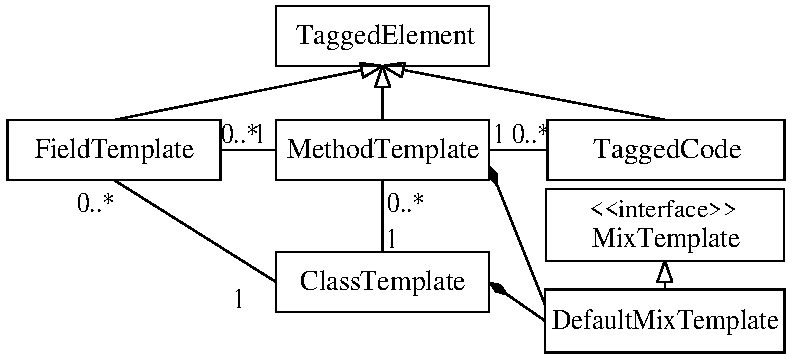
\includegraphics[width=8cm,height=!]{ch05/ct-ast2}
	\end{center}
	\caption{CT-AST API}
	\label{fig:ct-ast}
\end{figure}

Internally, the GAAST representation is organized around a class-based API called a \textit{Class Template AST (CT-AST)}, shown in \fig{fig:ct-ast}. The CT-AST API wraps the original AST of the source code \seec{ch05} and contains operations that facilitate the AST manipulation of classes and methods. For example, method bodies are represented as a list of attribute decorated \texttt{TaggedCode} elements divided into three logical blocks: begin, middle, and end (\fig{fig:method-body2}).

\begin{figure}[ht]
	\begin{center}
		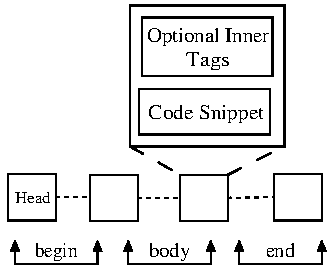
\includegraphics[width=5cm,height=!]{ch05/method-body2}
	\end{center}
	\caption{CT-AST Method Body Model}
	\label{fig:method-body2}
\end{figure}

This organization helps transformers to select code elements of interest based on attributes and to insert new code elements before or after any other code block. When an existing method is parsed in code, its method body is represented as a single code element in the middle block\footnote{All transformers of prototype for J2ME MIDP of \kr{ch05} work at the method block level.}. Each element of the CT-AST API derives from a {\tt Taggeg\-Ele\-ment} and can be decorated with one or more attributes \see{sec.inner.tags}. Support for merging different class templates is provided using a {\tt De\-fault\-Mix\-Tem\-pla\-te} class \see{sec.workflow}.

\begin{figure}[ht]
	\centering
	\begin{minipage}[b]{12cm}
	\begin{center}	
\begin{scriptsize}
\begin{lstlisting}[numbers=left,language=XML,frame=leftline]{}
<!ELEMENT methodbody (startblock?, middleblock?, endblock?) >
<!ELEMENT startblock (taggedcode)+ >
<!ELEMENT middleblock (taggedcode)+ >
<!ELEMENT endblock (taggedcode)+ >
<!ELEMENT taggedcode (tags?, code) >
<!ATTLIST taggedcode name CDATA #IMPLIED >
		\end{lstlisting}
		\end{scriptsize}
	\end{center}
	\caption{Tango's Internal Model of the Method Body}
	\label{c4f:tango.model}
	\end{minipage}	
\end{figure}

Internally, Tango works with an XML \cite{skonnardetal.01} representation of the CT-AST and expects the input to be converted to XML. For example, \fig{c4f:tango.model} shows how the method body is modeled in Tango as XML DTD. This enables more flexibility for processing code originating from more than one language, that conforms to the CT-AST meta-model. The internal XML representation externalizes the AST parsing outside Tango. The AST parsing can be done with any parsing or meta-programming tool\footnote{\Kr{ch05} explains how the real AST for J2ME MIDP is obtained.}.

\begin{figure}[ht]
		\centering
		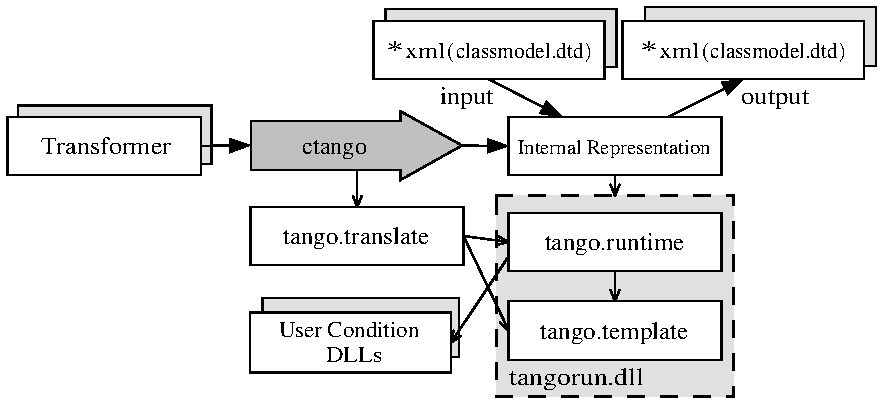
\includegraphics[width=10cm,height=!]{ch04/tango}
	\caption{Tango Framework}
	\label{fig:tango}
\end{figure}

The high-level organization of Tango is shown in \fig{fig:tango}. The usage of the XML representation is implicit in Tango. Tango supports a set of CT-AST classes around XML (part of \textit{tango.template} namespace in \fig{fig:tango}) similar to those in \fig{fig:method-body2}, that are used by the transformers. The node selection operations of Tango are internally mapped to XML queries using XPATH \cite{url.xpath}. The Tango processor (ctango) invokes the Tango run-time to process the input code encoded in the Tango's XML format. The transformation functionality is specified as input to the Tango processor. This functionality is first mapped onto the internal Tango representation in XML (\textit{tango.translate} namespace). The Tango processor invokes the Tango run-time (the transformation engine) that maps the input code to the output code based on the transformation logic\footnote{Custom user condition DLLs are explained in \sr{sec.tango.layers}.}.


\subsection{Class Transformations}
\label{attrib.trans}

Classes annotated with attributes serve as input units for attribute-driven transformers. \fig{fig:ch04tg} shows that an attribute annotated class can be transformed in two ways. A new class can be created, or the class can be modified in place\footnote{More than a single new class could be created. In-place class transformation and creation of the new classes can also be combined (see equation~\ref{eq.main}).}. The exact transformation will depend on the semantics that attributes carry and the specific invasive technology used.

\begin{figure}[ht]
		\centering
		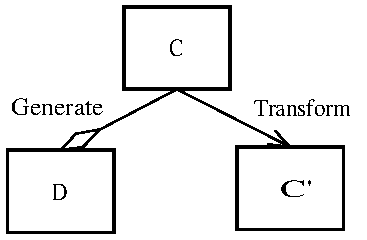
\includegraphics[width=4cm,height=!]{ch02/transgen}
	\caption{Transformation and Generation}
	\label{fig:ch04tg}
\end{figure}

\begin{itemize}
\item \textit{Creating a new class.} A class $C$ annotated with attributes is processed with a transformer $T$, giving a new class $D$, such that $D$ = $T(C)$. The $D$ class is called an adapter \cite{dpatterns}. The original class $C$ does not change. The adapter $D$ contains the additional functionality introduced by $T$, and forwards the messages as necessary to the original class $C$. Both, $D$ and $C$ must be present in the system. Another way to implement $D$ is based on the template pattern \cite{dpatterns}. In this view, $D$ is the result of the template $T$, where the specialization C is applied: $D$ = $T<C>$. The class $D$ is \textit{generated} based on the class $C$.

The implementation of $T$ requires that the $C$'s implementation is independent of the intended attribute semantics. This means that $C$ should be successfully compiled ignoring the attributes. This transformation in not possible for most attribute-based DSA. To maximize automation, attributes are used to introduce changes in the code before compilation.

The $D$ class can either be obtained before (or during) compilation, or at run-time using reflection when supported. For example, .NET saves structural attributes into the compiled binary. At run-time, annotations can be accessed using reflection. In .NET languages, rather than using the component $C$ directly, the implementation of $D$ can use reflection over the original component $C$\footnote{It becomes a bottleneck if a lot of reflection code is written every-time, unless an adapter pattern \cite{dpatterns} is used.}. Alternatively, $D$ can be generated before compilation using the .NET \textit{CodeDom API} \cite{cdom} over the component $C$'s source code. The adapter $D$ could also be changed dynamically resulting in some form of dynamic AOP \cite{kiczalesetal.97}\footnote{In this case, the rest of the program should be aware of the adapter $D$ and use it instead of using the class $C$ directly which may not be always acceptable.}.

\item \textit{In-place class modification.} The annotated class implementation is dependent on the semantics of the tags. $C$ could not be compiled directly without applying some transformation (add / remove code) to it. In this case, the attribute-based transformer $T$ gives a new class $C'$, such that $C'$ = $T(C)$. Only the class $C'$ must be present afterward in the system. The class $C$ is \textit{transformed} into the class $C'$.

In-place class modification supports invasive changes that need to be applied before compilation. These changes are needed to support attribute-based DSA, and when the original system is not designed with transformation in mind (and makes direct use of $C$, rather than through a new component $D$).
In-place class transformations are usually applied to source code, because generally the class $C$ can not be compiled directly.
\end{itemize}

\noindent The symbol $\Gamma$ will be used to stand for both $D$ and $C'$, when it not necessary to distinguish the two cases, that is $\Gamma$ = $T(C)$. If  $C$'s implementation supports non-invasive transformations, then $\Gamma$ could be either $D$ or $C'$ since both are possible, otherwise it is $C'$. $\Gamma$ is the result of the transformation process, that is, $\Gamma$ is the final implementation of $C$. $\Gamma$'s implementation is identified by the tuple $<T, C>$. The motivation to split $\Gamma$'s implementation is that the same transformer $T$ can be used for any class $C$ decorated with attributes that drive the $T$ transformation. This way, an entire set of classes $\{\Gamma\}$ is parameterized based on an implementation set $\{C\}$. $T$ can be seen as an implementation template, parameterized by $C$. The functionality of $T$ does not need to be repeated in every element of $\{\Gamma\}$.

Additional specialization parameters can be specified as a parameter vector $\Pi$ to T, that is $\Gamma$ = $T(\Pi, C)$. Parameters offer a convenient way to parameterize $T$ independently of the implementation of $\{C\}$. The representation $\Gamma$ = $T(\Pi, C)$ is very general. It can be implemented in various ways, e.g., using high-order functions \cite{mozart.04}, or generics (templates) \cite{generative.00}, depending on the hosting language technology. The focus will be on implementing $T$ for attribute-driven transformers, which usually apply in-place class modifications.

Implementation of attribute-based transformers is usually difficult, because more than a single attribute needs to be processed as part of a complex context. Usually an attribute-driven transformer $T$ takes as input a set of classes $\{C\}$ decorated with several attributes $\{\tau(\pi)\}$, where $\pi$ are the parameters of a single attribute $\tau$. Thus, an attribute transformer $T$ can be defined as a transformation function by the equation~\ref{eq.main}:

\begin{equation}
\{\Gamma\} = T(\{\tau(\pi)\}, \{C\})
\label{eq.main}
\end{equation}

\noindent The transformer $T$ in equation~\ref{eq.main} transforms a set of input classes $\{C\}$ decorated with a set of attributes $\{\tau(\pi)\}$ into a set of output classes $\{\Gamma\}$. The attribute set $\{\tau(\pi)\}$ is the \textit{coupling set} between $T$'s implementation and $\{C\}$.
%
The implementation of $C$ needs to be accessed inside the implementation of $T$, in order to be able to reason about it. Only the case when $C$ is source code will be considered in this chapter. Other transformation based on the same technology can be used for other representations of $C$, e.g., in the Java bytecode representation, if the possibility to access and manipulate similar entities exists in those other representations.

\subsection{Mapping Transformation Logic to Attribute Families}
\label{sec.tango.domain}

\Sr{attribute.families} explained how attribute families can be used as a variability mechanism for product-lines. Attribute families could also help to logically organize attribute-based DSA transformations. They drive the first modularization of $T$ in equation~\ref{eq.main}.

Each family of attributes can be processed by a single transformation unit specialized for that family. Formally, the entire attribute set $\{\tau(\pi)\}$ is split in a finite series of disjoint subsets $\phi_i$, corresponding to each attribute family $i$ in a domain of interest. The transformation function $T$ in equation~\ref{eq.main} can be then expressed as a composition of transformers $\Phi_i$ corresponding to the $N$ attribute families:

\begin{equation}
\{\Gamma\} = \Phi_1 \circ \dots \circ \Phi_N(\{\tau(\pi)\}, \{C\}) 
= \Phi_1(\phi_1, \{C\}) \circ \dots \circ \Phi_N(\phi_N, \{C\})
\label{eq.compose}
\end{equation}

All individual family transformers have access to all classes passed as input to $T$ and select the ones of interests based on their specific attributes $\phi_i$. The decomposition of each transformer $\Phi_i$ could be done similarly, if needed, based on attribute sub-families. The $\Phi_i$ transformers of individual attribute families can be organized as plug-ins of a generic attribute-driven transformation framework \seec{ch05}.

\subsection{Controlling Composition Semantics with Inner Tags}
\label{sec.inner.tags}

A side-effect of the equation~\ref{eq.compose} is that it removes the global transformation state that was preserved in $T$ (equation~\ref{eq.main}). There is no global way to maintain information about the overall transformation process. Results of previous computations should be explicitly passed to the next transformer in the chain. This can be done by means of additional parameters passed to each $\Phi_i$, or by encoding the information to pass in the transformed classes that result from the input $\{C\}$. Each transformer $\Phi_i(\phi_i, \{C_i\})$ needs to re-parse the information of the previous transformer $\{C_i\} = \Phi_{i - 1}(\phi_{i - 1}, \{C_{i - 1}\})$. Reprocessing the AST can be avoided, if the information that needs to be passed between the transformers is also encoded as attributes. Now, each transformer has the form $\Phi_i(\phi_i, I_i, \{C_i\})$, where $I_i$ are the additional attributes expected to be found in $\{C_i\}$ before the $\phi_i$-driven transformation can be applied. The $I_i$ attributes do not represent directly domain-level concepts as the $\phi_i$ do. When present, the $I_i$ attributes only help with the transformation concerns. The output $C'_i$ of each transformer $\Phi_i$ is decorated with a set of attributes $O_i$ made up of a combination of the unprocessed explicit attributes, and the $I_{i+1}$ phase attributes added during the $\Phi_i$ transformation:

\begin{equation}
(O_i, \{C'_i\}) = \Phi_i(\phi_i, I_i, \{C_i\})
\label{eq.trans}
\end{equation}

In Tango, the $I_i$ attributes are known as \textit{inner tags} (or attributes). Tango treats the inner tags as a natural extension of the explicit attributes, that enable a declarative transformer composition. Inner tags are used only in the inner operations of attribute-driven transformers and offer a convenient means for specifying the \textit{coupling sets} between the composed transformers, by removing the need to reinterpret the code. Inner tags are similar to ASF+SDF \cite{asfsdf.02} \textit{placeholders} for saving intermediate results. In Tango, the inner tags offer a uniform model to controll custom semantics, that is integrated uniformly with the remainder of attribute-driven transformer operations. Transformers deal with the inner tags in the same way they process the explicit attributes. All Tango's basic edit operations can specify inner tags to decorate the entities that they modify. 

\begin{figure}[ht]
		\centering
		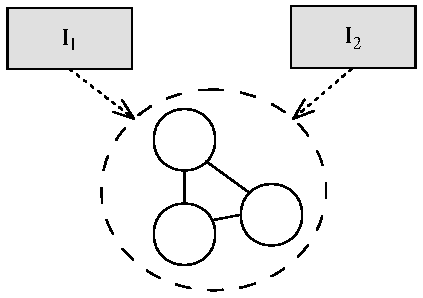
\includegraphics[width=5cm,height=!]{ch04/it-node}
	\caption{AST Node Grouping and Labeling with Inner Tags}
	\label{fig:it-node}
\end{figure}

While inner tags place transformer interaction semantics, the alternative is to reprocess the AST in each transformer, to check whether it fulfills a given condition. Using inner tags does not grow transformer coupling (it remains the same). Inner tags only make the coupling declarative, avoiding AST reprocessing. Logically, the inner tags are used to create arbitrary graph node sets \cite{mens.99}, which may not correspond directly to the generalized AST graph nesting structure as shown in \fig{fig:it-node}. A group of AST nodes is decorated with same inner tags to form a single logical node unit. Inner tags also help to associate more than one label with a node (group) as in \fig{fig:it-node}, in order to select the node in more than one logical set.

\begin{figure}[ht]
		\centering
		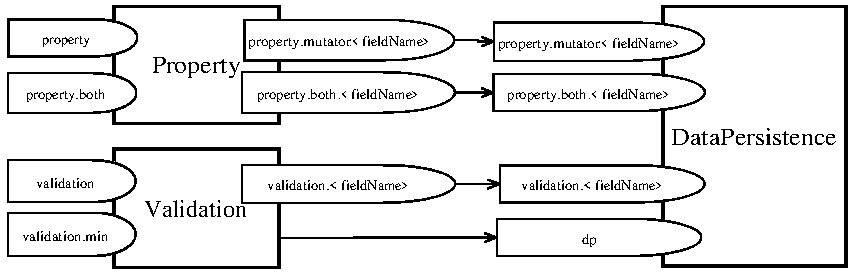
\includegraphics[width=12cm,height=!]{ch04/tcomp}
	\caption{Transformer Composition Based on Tags}
	\label{fig:tcomp}
\end{figure}

Consider again the attribute-driven transformation example of \fig{fig:input}, presented in \sr{attribute.families}.
\fig{fig:tcomp} shows a possible combination of the three attribute-driven transformers, namely, \texttt{Pro\-per\-ty}, \texttt{Va\-li\-da\-tion} and \texttt{Da\-ta\-Per\-si\-ste\-nce} for processing the code of the example in \fig{fig:input}. The exact combination order may change in a particular implementation.  In this example, the \texttt{Pro\-per\-ty} transformer  expects the input unit(s) to be decorated with attributes \texttt{property} and \texttt{property.both}. The \texttt{Pro\-per\-ty} transformer decorates its output, which is made of the added property methods, e.g., \texttt{set\-Sco\-re()}, and their corresponding fields, e.g., \texttt{score}, with a \texttt{pro\-per\-ty.mu\-ta\-tor.$<$field\-Na\-me$>$} inner tag (among the other tags). The \texttt{$<$field\-Na\-me$>$} in \fig{fig:tcomp}  stands for the actual field name, e.g., \texttt{score}. The actual value is expanded during the transformation process.

The \texttt{Da\-ta\-Per\-si\-ste\-nce} transformer combines the output of the two previous transformers.  \texttt{Da\-ta\-Per\-si\-ste\-nce} requires that the AST, it works upon, is decorated among the others with the (inner) tags \texttt{prope\-rty.both.$<$field\-Na\-me$>$} and \texttt{va\-li\-da\-tion.$<$field\-Na\-me$>$} to be able to read, modify, and validate the field data inside the persistence code that it adds. \texttt{Da\-ta\-Per\-si\-ste\-nce} treats the inner tags, e.g., \texttt{pro\-per\-ty.mu\-ta\-tor.$<$field\-Na\-me$>$}, in the same way it treats explicit attributes, e.g.,  \texttt{dp}, and cannot distinguish between the two.

\subsection{The Transformation Workflow}
\label{sec.workflow}

For the transformation of the equation~\ref{eq.compose} to be applicable in practice, a partial order over $\Phi_i$ should be found. The partial order of $\Phi_i$ depends (a) on the domain assets that $\Phi_i$ models, expressed by the attribute set $\phi_i$ and (b) on the details of the $\Phi_i$ implementation, expressed by the attribute set $I_i$. The implementation order is accidental, and the $I_i$ will depend on the order placed upon $\phi_i$. Because the transformers $\Phi_i$ model domain concerns, they can be named according to the concerns they address ($\Phi_i\rightarrow name$). The names of the $\Phi_i$ transformers can be used by the developers to define a partial order over $\Phi_i$. The process can be partially automated by specifying for each addressed domain concern, what other concerns need to be processed before and after it, as $\Phi_i\{before\} \{after\}$ lists. The elements of before and after lists are made of the $\Phi_i$ transformer names, or of special quantifier symbols, e.g., \textit{all} or \textit{any}. These local dependency relations are processed automatically to build the total $\Phi_i$ dependency graph, as shown in the example of \fig{fig.dependency}. Encoding the dependency relations locally in each transformer, rather than globally, is preferable, because the dependency relations depend on the particular implementation of the $\Phi_i$. The local encoding of dependencies frees the developers from having to build manually the total dependency graph.

\begin{figure}[ht]
		\centering
		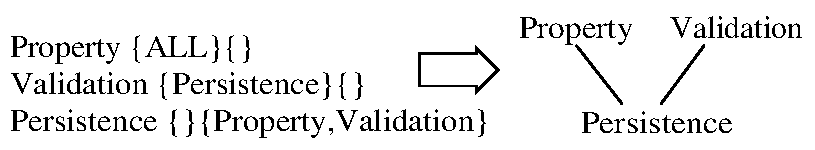
\includegraphics[width=8cm,height=!]{ch04/dependency}
	\caption{Resolving Dependencies}
	\label{fig.dependency}
\end{figure}
 
The dependency graph defines the transformation workflow. The developers can modify the automatically generated dependency graph manually to resolve any conflicts, on a case by case basis. A minimal workflow language is supported in Tango for this purpose. The Tango's workflow syntax is made up of (a) class variables ('\$') that can point to the processed classes, (b) constructors that create empty or initialized class variables, and operations to save them back to source files, (c) an operation to assign (deep copy) the class variables ('='), and (d) two composition operators:  the sequential composition (',') (which is equivalent to the function '()' operator) and the try operator ('$|$') that is similar to an 'if ... else' construct. A transformer in Tango, either succeeds or fails.

For example, the workflow order of the transformers of \fig{fig:tcomp} can be specified as \texttt{\$CT = Property, Validation, Persistence;} which is equivalent to \texttt{\$CT = Per\-si\-ste\-nce(Va\-li\-da\-tion(Pro\-pe\-rty(\$CT)));}. Actually both notations are supported. For the MIDP domain concerns addressed in this book, e.g., data \texttt{Per\-si\-sten\-ce}, it makes no sense to apply the transformations continuously to a class. For this reason, Tango, currently, does not define loops, or other more sophisticated workflow operations.

Once the dependency graph, based on the domain concerns, is in place, the inner tags are used inside the transformer implementations to coordinate the control flow inside the individual transformers. Sometimes \textit{transformation adapters} need to be created to process the input, so the code has the form and the inner tags expected by an existing transformer. The equation~\ref{eq.compose} leads to a sequential evaluation of transformers. However, based on the domain dependency graph, some of the $\Phi_i$ transformers could be orthogonal to the others and the parallelism ('$||$') could be explored: 

\begin{equation}
\{\Gamma\} = (\bigcirc, | |) \Phi_i(\phi_i, I_i, \{C_i\}), i \in {1,N}
\label{eq.par}
\end{equation}

For example, in \fig{fig:tcomp} the input AST for the \texttt{Da\-ta\-Per\-si\-ste\-nce} comes from two other transformers that could work in parallel \texttt{Pro\-per\-ty} and \texttt{Va\-li\-da\-tion}. The \texttt{Da\-ta\-Per\-si\-ste\-nce} transformer does not need to reevaluate the AST. It only checks for the required attributes. In this case \texttt{Da\-ta\-Per\-si\-ste\-nce} mixes also the output of \texttt{Pro\-per\-ty} and \texttt{Va\-li\-da\-tion} transformers. In this case, \texttt{Pro\-per\-ty} and \texttt{Va\-li\-da\-tion} could also be seen as adapters of the original AST, to make it suitable for further processing by the transformer \texttt{Da\-ta\-Per\-si\-ste\-nce}. All the composition semantics are represented as attribute names (labels) in \fig{fig:tcomp}.

Because of the parallelism, different versions of the same class could be present during the transformation, as in the case with the classes output by the \texttt{Pro\-per\-ty} and \texttt{Va\-li\-da\-tion} transformers. Because of the orthogonality of parallel transformers, these classes need to be merged. A default merge operation that returns the union of the members of two classes, and the union of corresponding method code blocks \see{sec.ast.tango} is provided in MobCon \see{sec.mc.wf}. More complicated class merging need to be coded manually inside a transformer. Tango generalizes the merging concept by allowing any combination of classes to be merged at once inside a transformer. This enables a uniform composition of the transformers, unlike other systems, e.g., JMangler \cite{jmangler}, that make a distinction between individual transformers and mergers. While Tango evaluates all transformers sequentially, threading and synchronization could be implemented automatically if needed, based on the data flow \cite{mozart.04} graph on the $\Phi_i$ transformer boundaries.   
 
\subsection{Layering the Transformation Strategy}
\label{sec.tango.layers}

Up to now, only the knowledge of the domain assets is used to enable a \textit{horizontal} modularization of the attribute-driven transformers \see{sec.tango.domain} and to define the transformation workflow \see{sec.workflow}. It is also possible to explore the features of the supported language meta-model to enable a \textit{vertical} modularization of the transformers. Tango uses a common OO meta-model based on classes, fields, methods, and method blocks. This hardwired OO meta-model is enough to support the transformations that mobile containers introduce in an OO mobile product-line \seec{ch05}. The specific features of the language meta-model have been used in the past to create customized solutions for specific sets of languages. For example, denotational semantics \cite{sem.99,apld.96} explore the features of procedural languages, in order to provide a specialized model for expressing and verifying language semantics, which applies better to procedural languages than the generic operational, or axiomatic semantics \cite{sem.99}.

\begin{figure}[ht]
		\centering
		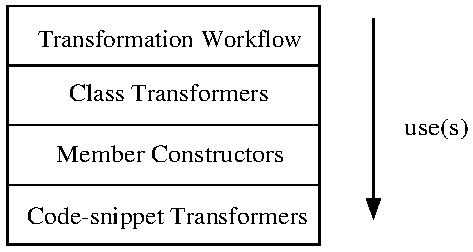
\includegraphics[width=6cm,height=!]{ch04/layers}
	\caption{Tango Framework Layers}
	\label{fig:layers}
\end{figure}

The structural information of the hardwired common OO meta-model can be used to structure the transformation \textit{strategy} \cite{stratego.01} in layers, corresponding to the nesting of the structural elements in the OO meta-model. Layering enables reasoning at different levels of abstraction about the transformation strategy, and enhances the reuse of the low-layer modules in more than one transformer. The attribute-transformers in Tango are organized in several hierarchical layers, shown in \fig{fig:layers}. The \textit{transformers workflow layer} was already discussed in \sr{sec.workflow}, the \textit{class transformers layer} ($T_c$) defines operations applied to classes, the \textit{member constructors layer} ($T_m$) defines operations applied to fields and methods, whereas the \textit{code snippets layer} ($T_s$) helps to manipulate the code templates that are used inside the method blocks. The transformer $\Phi_i$ of equation~\ref{eq.trans} can be written as:

\begin{equation}
\Phi_i(\phi_i, I_i, \{C\}) = T_{c_i}(\{C\},T_{m_i}(\{C_{members}\}, T_{s_i}(\{members_{code\_blocks}\}) ) )
\label{eq.layers}
\end{equation}

The information about $\phi_i$ and $I_i$ is distributed as needed between the transformers of each layer. The classes from \{C\} to be processed in $T_{ci}$ are again selected based on the $\phi_i$ and the $I_i$ attributes, as in $\Phi_i$. Layering is possible in Tango because the OO meta-model is hardwired, so the nesting of the structural elements is completely known. An open meta-model cannot be layered clearly with declarative constructs specialized for its elements. 

Tango enforces layering using special syntax. Every attribute-driven transformer implemented in Tango has to be modularized to conform to the layering of \fig{fig:layers}. Each layer uses the elements of the successive lower layer, but cannot create elements of the upper layer. For example, class templates are only created in the workflow layer. The class transformer layer can only modify the class templates, but cannot create new ones. To find out which class templates take part into a transformation, only the workflow layer needs to be examined. Similarly, member constructors are used in the class transformers layer only. Finally, code snippets are used only by the member constructors.

\begin{figure}[ht]
	\begin{center}
	\begin{minipage}[t]{10cm}
		\begin{scriptsize}
		\begin{lstlisting}[numbers=left,language=Java,frame=leftline]{}
transformer Property(~ct) {
precondition {
    if(not check(~ct, tags(["property"])))
         noapply;
}
action {
    $fields = select(~ct, FIELDS, tags(["property.*"]);
    if(check($fields, empty())) error;
    iterator($field in $fields) {
        if(check($field, tags(["property.accessor"])
            or tags(["property.both"])))
            add(~ct, METHOD, GetMethod($field),
                [tag(<"property.accessor", $field.name>)]);
        else if(check($field, tags(["property.mutator"])
            or tags(["property.both"])))
            add(~ct, METHOD, SetMethod($field),
                [tag(<"property.mutator.", $field.name>)]);
    }
}
return ~ct; // optional the first argument is returned
}		
		\end{lstlisting}
		\end{scriptsize}
		\end{minipage}
	\end{center}
	\caption{The Property Class Transformer Implementation}
	\label{fig:property}
\end{figure}

To understand how vertical layering is implemented beyond the workflow level, consider how the \textit{Property} attribute family transformer for the \textit{GameScore} example of \fig{fig:input} can be implemented. \fig{fig:property} shows the complete implementation of the \textit{Property} transformer (class transformers level) in Tango.
Each \textbf{class level transformer} operates in one or more class template variables, passed to it as arguments by the workflow layer, e.g., the \verb ~ ct at line 1 of the code shown in \fig{fig:property}. The class level transformers cannot create new class templates. If new class templates need to be created, this has to be done at the workflow level. 

A class level transformer in Tango has two main parts: an optional \textit{precondition} part (lines 2 - 5) and an \textit{action} part (lines 6 - 19) (\fig{fig:property}). The optional precondition section is used to apply some quick checks on the input, in order to decide whether the transformation can be applied or not. Only non-edit operations are allowed in the precondition section. Tango preconditions are \textit{optimistic}. The action part can apply more specific checks, and the transformer may still fail as a consequence of a failed condition in the action part, even thought the preconditions succeeded. The precondition section is only aimed at being able to quickly determine the attribute family, or the main inner tag families, supported by the class transformer. Preconditions are not performance optimizations rather, they give a clue about the attribute family semantics addressed by the transformer. Preconditions remove the need to consult the more complex action section, when only a high-level view inside the functionality of a class transformer is needed. The \textit{noapply} operator (line 4) tells the Tango workflow that this transformer cannot be applied. If a transformer fails to apply, the control is returned to the workflow. Theoretically, a pre-condition and a post-condition  can be defined for any graph rewriting operation \cite{mens.99}, but in practice, it is cumbersome to enumerate them for each operation (post-conditions can be written as preconditions \cite{mens.99}), so only important checks are applied in the preconditions part in Tango.

The AST editing operations are allowed only in the \textit{action} part. The action part (lines 6 - 19) will modify the input class template, to add getter and setter methods for all fields decorated with an attribute belonging the \textit{property} family. The fields are selected in line 7 and stored as a list in the variable {\tt \$fields}. The generic \textit{select} operation is used to filter a set of nodes of the same type that fulfill a given condition. Only predefined types of the supported meta-model, e.g., {\tt FIELDS, ME\-THODS}, can be used. The third argument of \textit{select} is a \textit{condition}. Several predefined conditions are supported:
\begin{itemize}
\item 'tag' - filters AST nodes based on attributes,
\item 'name' - filters AST nodes based on names,
\item 'empty' - checks whether a node list is empty,
\item 'count' - checks the number of list items.
\end{itemize}

For conditions that expect string arguments, regular expressions are supported. Users can define additional custom conditions by implementing a required interface \texttt{IUser\-Con\-di\-tion} and packing the condition logic as a separate DLL placed in a predefined sub-folder. Every time the Tango's run-time finds an unknown condition name, the run-time searches whether a custom condition DLL with the same name can be found. If found, the DLL is loaded and the \texttt{IUser\-Con\-di\-tion} interface is used to invoke a generic {\tt Fil\-ter} method using reflection. Any argument list for the condition is passed to the {\tt Fil\-ter} method. The {\tt Fil\-ter} method returns a filtered list. If no such DLL is found, or an exception occurs when the DLL is invoked, an error is reported.

The \textit{check} operation in line 8 is similar to \textit{select}. It applies all the conditions passed to it as the first argument and returns a \textit{Boolean} value indicating whether conditions have succeeded or not. The individual conditions can be combined using Boolean operators: {\tt and, or, not}. The \textit{check} and \textit{select} operations pass the first argument implicitly to all conditions. This makes it easier to understand what a \textit{check} or \textit{select} statement does, given that all conditions work on the first argument of \textit{check} or \textit{select}\footnote{At the cost of a slightly slower implementation, since each condition has to re-iterate through the input list. Set operations are used to mix the results of different conditions: \texttt{and} corresponding to \textit{intersection}, \texttt{or} corresponding to \textit{union}, and \texttt{not} corresponding to set \textit{difference}. Given that \texttt{not} operation is easier to implement during iteration, the \texttt{Fil\-ter} method of the \texttt{IUser\-Condi\-tion} interface, accepts a special boolean flag indicating the \texttt{not} condition.}, and is similar to the concept of \textit{conventional interfaces} in \cite{sicp.96}\footnote{\url{http://mitpress.mit.edu/sicp/full-text/book/book-Z-H-15.html\#\%25_sec_2.2.3}}.

The iterations over the meta-model AST are divided between the \textit{check}, \textit{select}, and \textit{iterator}. The \textit{check} and \textit{select} operators do implicit iterations over \textit{finite} lists of elements (via the conditions). The \textit{iterator} operation in line 9 is used to apply an operation to all the elements of a list. The \textit{iterator} and \textit{select} could be a single operation, however, it makes sense to separate these operations in cases when lists, other than those returned by \textit{select}, are processed. 

The \textit{add} operation (lines 12 and 16) is an example of an edit operation. It adds a meta-element to the class template given as its first argument. The {\tt Get\-Me\-thod} and {\tt Set\-Me\-thod} are member constructors. All supported edit operations in the class transformers layer, i.e., \textit{add}, \textit{delete} and \textit{modify}, work upon class templates and use member constructors of the next lower layer. In the example of \fig{fig:property}, the \textit{add} operation also appends an inner tag to the newly added element: \texttt{[tag(<"pro\-pe\-rty.acce\-ssor", \$field.na\-me>)]}. The tag is created by the explicit attribute constructor \textit{tag}, combining the field tag type and the field name, by using the string concatenation operation \verb@<...>@. This inner tag can be used later in a \textit{select}, or \textit{check} statement of another transformer in the same way as an explicit attribute.

The \textit{add} and \textit{select} operations use a common pattern. The type of processed meta-elements is given explicitly. This improves the readability of the code (in the case of \textit{add}, the type could have been deduced from the member constructor type). An alternative would be to have distinct operation names for each meta-element type, e.g., \textit{addMethod}. This would then require to maintain the Tango parser if its supported language meta-model is customized. The modified class template is returned in line 20. %For an implementation of the two other transformers of this example consult \cite{tango.04}.

The \textbf{member constructors} layer defines the actual meta-model member implementations that are used in the class transformers layer. Class templates cannot be passed as arguments to the member constructors. Currently, Tango defines member constructors for fields, methods and tags. As explained in \sr{sec.ast.tango}, method bodies are represented as a list of attribute decorated code snippets divided into three logical blocks: begin, middle, and end (\fig{fig:method-body2}). This representation enables to quickly add or remove blocks of code to a method, without dealing directly with the AST node composition. All the changes that the attribute-based DSA for mobile containers introduce, modify the method internals at the block level only.

\begin{figure}[ht]
\begin{center}
\begin{minipage}{7cm}
\begin{scriptsize}
\begin{lstlisting}[numbers=left,language=Java,frame=leftline]{}
method ToRecord($fieldArray) {
  methodName(makeMethodName(["toRecord"]));
  methodReturn(ByteArray());
  addBody(StoreFields($fieldArray));
}
\end{lstlisting}
\end{scriptsize}
\end{minipage}
\end{center}
	\caption{Method Constructor Example}
	\label{fig:method}
\end{figure}

\fig{fig:method} shows a method member constructor \texttt{To\-Re\-cord}, that is used in the persistence transformer. The constructor expects an array of fields that will be serialized in a byte array, and returns the implementation of a method \texttt{toRecord} that takes care of the serialization. The method name for the newly created method is set in line 2, and its return type is set in line 4. The example specifies the method return type by invoking a code-snippet constructor \textit{ByteArray} (line 3). A code block is added in the middle block of the method, by using the \texttt{addBody} statement in line 4. The \texttt{addBody} invokes another code snippet constructor namely, \textit{StoreFields}, to obtain the code that implements the field serialization. The method body is produced by the code snippet constructor \textit{StoreFields} (\fig{fig:code}). The \textit{addBody} operation adds this code snippet at the end of the middle block list. No direct code is manipulated in this layer. Instead the code-snippet constructors, e.g., \textit{ByteArray} and \textit{StoreFields}, are called.

\subsection{Code-Snippet Templates}

\Sr{ch2:inv} explained that invasive techniques lead to writing more code because of the meta-level indirection of the programming model. The situation can be improved by using code templates \cite{voelter.generation,java.compost}. Attribute-based DSA modify the components they decorate. Most of the changes happen inside the method boundaries, or by adding new methods. Code templates can help (a) to reduce coding efforts inside the member constructors layer and (b) to isolate the rest of an attribute-driven transformer from the language specific details.

In Tango, the transformation abstractions are isolated from the remainder of the transformer implementation via the concept of a \textit{code snippet}\footnote{This term is borrowed from .NET CodeDom API \cite{cdom}.}, which is similar to Stratego's \cite{stratego.01} \textit{concrete syntax}. A code snippet is a source code node that Tango treats as a string. It is the only part of code which depends on the concrete syntax of programming language, where the code being transformed is written. The rest of a transformer's implementation in Tango works with the hardwired OO model. Code snippets enable the representation of parameterized clusters of the source code graph in the remainder of the transformer implementation, without having to deal with details of the AST nodes.

Tango requires that a particular implementation of the code-snippet templates has a way to replace parameters inside the code snippet. An example of a template code snippet, that makes use of the Apache Velocity \cite{velocity} script language, is shown in \fig{fig:code}. The code generates a possible implementation for the body of the \textit{toRecord} method shown in \fig{fig:output}, and that was used in the example of \fig{fig:method}.

\begin{figure}[ht]
	\centering
	\begin{minipage}[b]{8.5cm}
	\begin{center}	
\begin{scriptsize}
\begin{lstlisting}[numbers=left,language=Java,frame=leftline]{}
code StoreFields ($fieldArray) language (Velocity) {
    ByteArrayOutputStream baos = new ByteArrayOutputStream();
    DataOutputStream outputStream = new DataOutputStream(baos);
    #foreach($field in $fieldArray)
    outputStream.$dp_write($field.type)
        (this.$Tango.makeMethodName(["get", $field.name]()));
    #end
    return baos.toByteArray();
    #macro(dp_write, $type)
        if($type == string) UTF
        if($type == int) Int
    #end
}
		\end{lstlisting}
		\end{scriptsize}
	\end{center}
	\caption{Code Snippet Example}
	\label{fig:code}
\end{minipage}	
\end{figure}

The code of \fig{fig:code} is a Velocity string template specialized using the values in the \texttt{field\-Array} argument at line 1. A \texttt{Byte\-Array\-Output\-Stream} is created and used to initialize a \texttt{Data\-Output\-Stream}, so that the fields can be output formatted according to their type. The specialization is done in lines 4 - 7, which generate code to store each field of the class, in line 5. A special macro named \texttt{dp\_write}, defined in lines 9 - 12, is deployed to generate the right name of the \texttt{Data\-Output\-Stream} function, depending on the variable type. Only \textit{Inte\-gers} and \textit{Strings} are shown in this example. Strings data are saved using a portable UTF\footnote{Unicode Transformation Formats. \url{http://www.unicode.org/}} encoding.% The details of Velocity language are, however, outside the scope of this work.

\subsection{Termination}
\label{sec.tango.terminate}

The attribute-based transformation approach presented in this section can be considered as an instance of a \textit{graph rewriting system} (GRS) \cite{term.rewrite,Nagl:96,ehrig96computing,Blostein-Schuerr02:99,schuerr.95,schurr.graph.94,gr.99,assmann.00,Plump.2001}. Attributes form a finite vocabulary (\textit{signature}) used to transform a finite number of variables, represented as classes of an OO language. The approach can be seen as a form of graph labeling \cite{Plump.95,mens.99}, where labels form a \textit{hypergraph} \cite{Plump.95} made of attribute family trees. The explicit, and a part of the inner attributes, can be simplified to source code as a ground form. Some of the inner attributes, such as those used to support traceability \see{sec.tango.trace}, are \textit{irreducible} and are preserved in the final normalized form (source code).  

In terms of \cite{term.rewrite}, the approach is not convergent, as the order of transformation matters. That is, not all possible combinations of sequences of rules lead to the same normal form. The ordering or rules, however, ensures \textit{termination} \cite{Gramlich.96}. Termination is ensured for a relation if its transitive closure forms a well-founded ordering (definition 12 in \cite{term.rewrite}). The approach presented here has such a well-founded termination ordering. In the top level, the order of the transformation is ensured by the dependencies between the domain assets, forming a stratified \cite{datalog.89,assmann.00} structure for applying transformers. The workflow graph is finite and contains no endless substitution chains. Explicit loops are not allowed in the workflow syntax, whereas recursive, or circular transformer dependencies cannot appear, because the vertical transformation order is made up of a well-defined finite number of three hierarchical \cite{Ohlebusch.01} expanding levels: classes, methods, and method blocks. Rules of each level cannot refer to the parent, or the sibling rules, which prevents the circular dependencies\footnote{Infinite loops in the lowest code-snippet layer indicate programming errors.}.

In \cite{Assmann.94,Assmann.96} termination criteria are defined for special forms of GRSs, based on labeled graphs ($\Sigma-Graphs$). A series of derivations is finite, if it contains a finite number of finite derivations steps. Termination is warranted for the GRSs that contain only graph edge accumulation, called edge-addition rewrite systems (EARS). Furthermore, termination criteria are also specified for exhaustive GRSs (XGRS), made up of additive GRSs (AGRS) and subtractive GRSs (SGRS). The attribute-driven transformation presented here could contain subtractive operations, however, in practice changes are always additive (AGRS) and complement the original code of the annotated components.

The termination of hypergraph transformations in GRSs is discussed in \cite{Plump.95}, where a rule is defined as a combination of a left-side and a right-side graph morphisms. A forward closure is defined as a minimal set of successive derivation steps. Termination is warranted when the GRS consumes a rule in each step, and does not admit to an infinite forward closure. The attribute-driven transformations of this section, consume at least one attribute in each step, and because of the finite ordering, the derivation sequence is finite.

\subsection{Transformation Traceability}
\label{sec.tango.trace}

Traceability is important for generative frameworks because in Tango the code snippets replacements are not fully statically checked at the time of the string replacement. Rather, this action is postponed until the compilation time, where any possible errors will appear. These errors need to be connected back with the input code locations. Decoration with inner tags, in order to enable traceability logging, helps to deal with error tracing\footnote{Yacc \cite{yacc} solves this issue with ANSI C pragma directives that overwrite the line numbers in the outputted source file. This technique does not work with Java and .NET compilers. Furthermore, Tango transformers can carry out complex transformations and line number based traceability may not work in all cases.}.

\begin{figure}[ht]
		\centering
		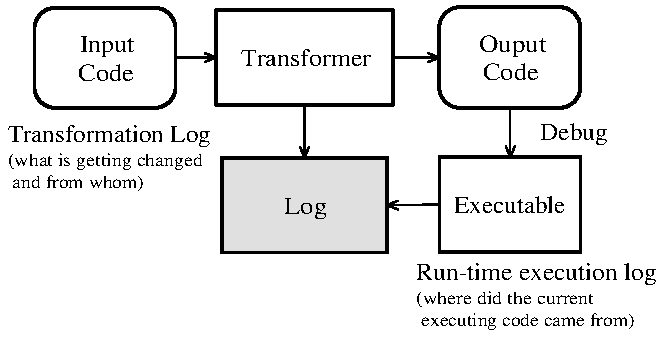
\includegraphics[width=10cm,height=!]{ch04/log}
	\caption{Transformation and Execution Log}
	\label{fig:ch04log}
\end{figure}

Traceability is integrated in the Tango framework (\fig{fig:ch04log}), and is implemented with the help of the inner attributes. Tango distinguishes between (a) transformation time log and (b) run-time execution log. The transformation log gives feedback about the transformation process. The execution log helps to trace the origin of the executed code. Traceability can be turned on and off for pieces of source code of interest by using a special explicit attribute \texttt{log}, directly in source code. When present, this attribute instructs the framework to automatically add special log calls to all methods that are transformed by every Tango transformer. The log calls are decorated with special attributes, that contain the transformer names which have edited a given method. When output code is executed, the log trace statements are printed on the console, enabling the display of the exact transformation history for each executing method (an example is given in \fig{fig:mobray}). This centralized tracing capability helps to debug the transformation-related side-effects.

As discussed in \kr{ch03}, GAAST languages support the preservation of the MDA PIM architecture into the PSM, when the PSM is source code, shifting the model transformation to the language level. The structured attribute-driven transformations of this chapter further preserve the traceability of the PIM, after the PSM transformation. Inner attributes \see{sec.inner.tags} enable the association of traceability semantics with the transformed elements. The Tango framework preserves the inner attributes in the outputted code. This approach enables tracing back the origin of the code and depending on the design of the transformers\footnote{For example, MobCon \seec{ch05} transformers are additive. They never remove the original user code from the transformed components, only append to it. This ensures complete traceability when combined with the preservation of the inner attributes.} and the redundancy of the used inner attributes, it could also used to support full round-trip engineering. The preserved inner attributes do not influence the performance of the end system. The representation of the inner attributes could also be combined with specific language support for attributes, as in the case of Java 1.5 \see{when.annotate}, to directly support traceability at run-time.


\section{Automating Attribute Transformation Concerns}
\label{ch04:sec:dep}

The transformation process for interpreting the attribute-based DSA was modularized in \sr{sec.attribute.trans} based on the domain assets. Several transformation related issues, e.g., checking for the right usage of attributes, or validating the AST to conform to the decorated attributes, must still be implemented separately in each transformer. There are many repetitive transformation concerns that crosscut more than one attribute-driven transformation. The repetite transformation concerns can be factored out from the individual $\Phi_i$ transformers, and implemented as generic attribute-driven operations $\Delta_j(\{\tau(\pi)\}, \{C\})$.  The equation~\ref{eq.par} becomes \ref{eq.ccc1}, with the $\Phi_i$-s simplified by the $\Delta_j$-s. 

\begin{equation}
\{\Gamma\} = (\bigcirc, ||)[\Delta_j(\{\tau(\pi)\}, \{C\}), \Phi_i(\phi_i, I_i, \{C_i\})]
\label{eq.ccc1}
\end{equation}

\noindent The transformation cross-cutting concerns $\Delta_j$ are candidates to be handled automatically by an attribute-driven transformation framework. For example, logging \see{sec.tango.trace} is a cross-cutting concern handled automatically by the Tango framework as part of the traceability. This section demonstrates a generic technique that can help to factor out declaratively the cross-cutting functionality $\Delta_j$, outside of the individual $\Phi_i$ transformers. To illustrate the concept, two examples of cross-cutting attribute transformation concerns are considered next.

\textbf{ I) Attribute dependencies.} In \sr{sec:var.dsa}, an example of how a web service can be modeled with DSA was given. \fig{fig:webservice-dsl} is repeated here for convenience as \fig{fig:webservice-dsl-2}. \Sr{c2.sec.dsa.attributes} illustrated how the same web service DSA can be modeled with attributes in \fig{fig:webservice}, repeated here as \fig{fig:webservice-2}.

\begin{figure}[ht]
\begin{minipage}[t]{0.4\linewidth}
\begin{center}
\begin{scriptsize}
\begin{lstlisting}[numbers=left,language=Java,frame=leftline]{}
webservice TravelAgent {
  ...
  webmethod GetHotels(){...}
  ...
}
\end{lstlisting}
\end{scriptsize}
\vspace{0.7cm}
\end{center}
\caption{A Domain-specific Extension to Implement Web Services (\fig{fig:webservice-dsl})}
\label{fig:webservice-dsl-2}\end{minipage}\hspace{1cm}%
\begin{minipage}[t]{0.4\linewidth}
\begin{center}
\begin{scriptsize}
\begin{lstlisting}[numbers=left,language=Java,frame=leftline]{}
[WebService]
class TravelAgent {
  ...
  [WebMethod]
  public void GetHotels(){...}
  ...
}
\end{lstlisting}
\end{scriptsize}
\end{center}
\caption{A Web Service Class with two Inter-depended Attributes (\fig{fig:webservice})}
\label{fig:webservice-2}\end{minipage}
\end{figure}

When a DSL (or EDSL) is used, an explicit grammar rule, such as, \texttt{web\-ser\-vi\-ce := web\-me\-thod+}, explicitly defines the context relation between \texttt{web\-ser\-vi\-ce} and \texttt{webme\-thod} in \fig{fig:webservice-dsl-2}. 
A web method will appear only inside a web service and vice-versa, a web service will contain web methods. This grammar rule is automatically enforced by the parser.
 
When attribute-based DSA are used, there is no default way how such a generic dependency constrain can be declared and enforced. It remains the responsibility of the corresponding attribute transformer to validate the dependency constrain. Depending on whether the class or its methods are considered, there are two constrains that need to be enforced: (a) public methods of a class decorated with \texttt{[Web\-Servi\-ce]} should be decorated with the \texttt{[Web\-Method]} attribute\footnote{For simplicity, it is assumed that all public methods need to be decorated. The actual implementation explained in \sr{sec:adc} removes this restriction by enabling user-defined filters for specifying which code elements, in this case methods, will be checked and which will be not.}, (b) any method decorated with a \texttt{[Web\-Method]} attribute should be declared within a class decorated with the \texttt{[Web\-Servi\-ce]} attribute. That is, the two attributes are inter-dependent. The dependency relation needs not to be symmetric, e.g., a \texttt{[Va\-li\-da\-te]} attribute may require another \texttt{[Va\-li\-da\-te.Max\-Va\-lue]} attribute, whereas the \texttt{[Va\-li\-da\-te.Max\-Va\-lue]} attribute may also be used alone.

Checking attribute dependencies is needed in any attribute family transformer, in order to make sure, for example, that suitable sub-attributes have been used. The code required to enforce dependencies between attributes, stating, for example, that a certain attribute is present in the program hierarchy before another attribute can be used, is a cross-cutting concern (CCC) that is repeated in every transformer.

\textbf{II) Virtual instances and \texttt{this} keyword usage.} This example is motivated by the implementation restrictions of the EJB \cite{www.ejb} programming model. The EJB specification states, among other restrictions, that components whose instances are managed as \textit{virtual instances} \cite{server.patterns.02} should not pass \textit{this} as a parameter or as method return value. The underlying rationale is that it makes no sense to return a direct pointer to an object that will be reused with a different internal state, at a later point of time, by the container. While the EJB implementations up to version 2.1 do not rely on attributes, Java 1.5 annotations will be used in EJB 3.0 \cite{ejb30} instead of the marking interfaces \see{attributes}.

\begin{figure}[ht]
	\begin{center}
	\begin{minipage}{5cm}
	\begin{scriptsize}
\begin{lstlisting}[numbers=left,language=Java,frame=leftline]{}
[VirtualInstance]
class C {
  ...
  [InitInstance]
  public C initialize(Id id){...}
  ...
}
\end{lstlisting}
\end{scriptsize}
\end{minipage}
\end{center}
\caption{A Class that Requires Virtual Instance Support}
\label{fig:vinstance}
\end{figure}

The imaginary example shown in \fig{fig:vinstance} supposes that the lifetime of an instance of a class \texttt{C} is going to be managed by the container, only when the class declaration is decorated with the attribute \texttt{[Vir\-tual\-Insta\-nce]}. For a class \texttt{C} tagged with the attribute \texttt{[Vir\-tual\-Insta\-nce]}, the restriction about \textit{this} must hold. The method \texttt{initialize()} of class \texttt{C} is invoked by the container when a virtual instance needs to be initialized. This method is identified by annotating it with an \texttt{[Init\-Instan\-ce]} attribute to distinguish it for later processing.

The transformer of the \texttt{[Vir\-tualInsta\-nce]} attribute needs to check the \textit{no-this} restriction for the methods that the class contains. The same check could be repeated in the member constructor transformer for the \texttt{initialize()} method, which processes the \texttt{[Init\-Instan\-ce]} attribute. Transformers for other domain assets, e.g., database connection pooling transformers, may also need to check the \textit{no-this} restriction. The same validation code needs to be repeated in different transformers for the AST blocks inside a method.

\subsection{Expressing Cross-Cutting Concerns with Meta-Attributes}

In a GAAST language \see{sec:gaast}, all entities can be decorated with attributes. \textit{Meta-attributes} are attributes used to decorate other attributes. Meta-attributes can be used to associate arbitrary semantics with attributes that can be checked for, or enforced automatically. Meta-attributes do not decorate attribute instantiation\footnote{Attribute parameters \see{ch03:sec:attrib.param} are used to express the variability of the attribute instantiation.}. Rather meta-attributes decorate attribute definitions. When an attribute $\tau(\pi)$ is defined, its definition is decorated with meta-attributes $\{\mu(\mu_{\pi})\}$, where $\mu_{\pi}$ are parameters used to specialize the meta-attribute instantiation. 
%
Meta-attributes provide a native mechanism to declaratively model the transformation cross-cutting concerns in GAAST languages. Meta-attributes help to factor the code that handles the cross-cutting concerns out of individual transformers, in generic concern processing tools, which can be made part of an attribute-driven transformation framework. The generic $\Delta_j$ transformers, working over meta-attributes $\{\mu(\mu_{\pi})\}$, can be expressed as in equation~\ref{eq.delta}. The $\{\mu(\mu_{\pi})\}$ define semantic constrains (or operations) that must hold over $\{\tau(\pi)\}$, when $\{\tau(\pi)\}$ are applied to $\{C\}$.

\begin{equation}
\Delta_j \rightarrow \Delta_j([\{\mu(\mu_{\pi})\},\{\tau(\pi)\}], \{C\})
\label{eq.delta}
\end{equation}

Using custom meta-attributes in .NET \cite{www.dotnet} is similar to using the predefined \texttt{[Sy\-stem.\-Attri\-bu\-te\-Usa\-ge\-Attri\-bu\-te]}. This special attribute is used in .NET to decorate the definition of a custom attribute, providing information about the lexical scope in which the attribute at hand can be used. Based on the usage attributes, every time a custom attribute is encountered in a program, the compiler can check whether the attribute is being used in the right lexical context, and report an error when this is not the case. The idea underlying \texttt{[Sy\-stem.\-Attri\-bu\-te\-Usa\-ge\-Attri\-bu\-te]} can be adopted to introduce new custom checks by using custom meta-attributes. 

\begin{figure}[ht]
	\begin{center}
	\begin{minipage}{12cm}
	\begin{scriptsize}
\begin{lstlisting}[numbers=left,language=Java,frame=leftline]{}
[AttributeUsage(AttributeTargets.Class)]
class NoThis : System.Attribute { ... }

[NoThis]
[AttributeUsage(AttributeTargets.Class)]
class VirtualInstance : System.Attribute { ... }

[NoThis]
[AttributeUsage(AttributeTargets.Method)]
class InitInstance : System.Attribute { ... }
\end{lstlisting}
\end{scriptsize}
\end{minipage}
\end{center}
\caption{Modeling \texttt{[NoThis]} Constraint as a Meta-Attribute}
\label{fig:no-this}
\end{figure}

Consider for example, the \textit{no-this} restriction \see{ch04:sec:dep} modeled as a \texttt{[No\-This]} me\-ta-attri\-bu\-te. The \texttt{[No\-This]} meta-attribute is used to decorate the definition of all attributes that need to check, or enforce, the \textit{no-this} constrain, as shown in the .NET C\# example of \fig{fig:no-this}. A cross-cutting attribute checker tool, that enforces the \textit{no-this} restriction, needs to check each attribute of a code entity, whether the attribute definition\footnote{Whether the attributes of the attribute itself.} contains a \texttt{[No\-This]} (meta-) attribute. If the condition is fulfilled, then the methods decorated with the corresponding attribute need to be checked. The cross-cutting concern checker tools operate outside the $\Phi_i$ transformers, reducing the amount of code that needs to be implemented and debugged in each individual $\Phi_i$ transformer.

The \textit{attribute dependency} example \see{ch04:sec:dep} is more complex, as it requires a bigger context to be handled, when the attribute dependencies are resolved. Ideally, it is preferable to declare the attribute dependencies similarly to grammar rules. Meta-attributes enable expressing attribute dependencies declaratively in GAAST languages. The rest of this section explores in detail how attribute dependencies can be modeled as meta-attributes and how they can be enforced automatically. The presented implementation is based on .NET \cite{www.dotnet}. The details of the attribute processing in .NET were discussed in \sr{c3.sec.dnet}.

Using meta-attributes frees the developers that write attribute-driven transformers from coding repeated concerns, by centralizing the way cross-cutting concerns are processed. The developers only declare constrains, e.g., dependencies, without taking explicitly care of how the corresponding concerns are resolved and enforced. 
There are of course many ways \see{sec.c4.related} to declare and enforce architectural dependencies \cite{minsky.98}. Using meta-attributes to decorate other attributes is a natural way for GAAST-like languages, because meta-attributes could be directly processed by the attribute-driven transformers presented in this chapter. 

\subsection{The Attribute Dependency Model}
\label{sec:model}

The attribute dependency model presented in this section distinguishes between (a) \textit{required} dependencies, stating that a given attribute requires another one in order to be used, and (b) \textit{disallowed} dependencies, stating that a given attribute cannot be used, if another attribute is present. 
Furthermore, children nodes in a program's structural hierarchy can declare dependency constrains on parents of any level, and vice-versa. 
An attribute of a certain program element instance may require that certain attributes are present in the set of the attributes of the structural children of its program element. For example, an attribute of a $Class$ may require that a certain attribute be present in the annotation of the class' $Methods$. The attribute dependency model generalizes these notions to any depth of the structural tree. %The reverse is also true. An attribute of a child structural element instance may require a certain attribute to be present in the set of the attributes specified for the parent instance. 

A restriction in this model is that the attributes of a program element instance cannot place any constraint on the attributes of sibling instances. For example, the attributes that a $Field$ instance is decorated with, cannot imply anything about the attributes of $Method$ instances, or attributes of other $Field$ instances. In the prototype for the J2ME MIDP \seec{ch05} sibling dependences are not used. However, the attributes of a program element instance can place constrains on the other attributes of the same instance. For example, a method attribute $a_{m1}$ of a method $m$ may require that another attribute $a_{m2}$ to be present for $m$. A more generic dependency model could be created (to include siblings constrains), but the more detailed semantics add nothing new to the meta-attribute concepts discussed.

The semantics of the $disallowed$ relation on the structural AST elements and instances can be specified similarly and will not be repeated.

\subsection{The \texttt{[DependencyAttribute]} Class}

.NET custom attributes are classes derived from the class \texttt{Sy\-stem.Attri\-bu\-te} \see{c3.sec.dnet}. Custom attributes may have arguments specified either as constructor parameters (unnamed arguments), or as properties of the attribute class, which generate \textit{getter} and \textit{setter} methods in C\# (named arguments). Attribute classes may also contain methods and state (instance fields), as every other .NET class does.
Using properties to specify attribute arguments is more flexible than using constructors, because .NET does not support complex types to be passed as parameters to the constructors\footnote{Only basic constant types and \texttt{Sy\-stem.Ty\-pe} can be used. \texttt{Sy\-stem.\-Object} is also listed in the documentation, because it is the parent of simple types and of \texttt{Sy\-stem.Ty\-pe}. This does not mean that arbitrary objects can be passed as constructor parameters.}. 

To handle the attribute dependencies, a new meta-attribute named  \texttt{De\-pen\-dency\-Attri\-bu\-te}\footnote{When used in code the suffix \texttt{Attri\-bu\-te} may be omitted from the name of an attribute class.} is defined as a custom attribute class. The \texttt{De\-pen\-dency\-Attri\-bu\-te} contains one \texttt{Re\-quired*} and one \texttt{Dis\-allowed*} property for every program element type, for which the attribute dependency checking is supported (\texttt{Assembly}\footnote{A .NET \texttt{Assembly} maps roughly to a Java JAR file. The \texttt{Assembly} attributes map roughly to custom JAR manifest entries.}, \texttt{Class}, \texttt{Me\-thod}), as shown in \fig{fig:da}. 
Given that the number of the node types in a program's structural tree is limited, it makes sense to enumerate such operations. This makes the code easier to understand compared to having a single dependency property for all meta-element types.

\begin{figure}[ht]
\begin{center}
\begin{minipage}{10cm}
\begin{scriptsize}
\begin{lstlisting}[numbers=left,language=Java,frame=leftline]{}
[AttributeUsage(AttributeTargets.Class)]
public class DependencyAttribute : System.Attribute {
  ...
  public DependencyAttribute() {...}
  public Type[] RequiredAssemblyAttributes {...}
  public Type[] DisallowedAssemblyAttributes {...}
  public Type[] RequiredClassAttributes {...}
  public Type[] DisallowedClassAttributes	{...}
  public Type[] RequiredMethodAttributes {...}
  public Type[] DisallowedMethodAttributes {...}
}
\end{lstlisting}
\end{scriptsize}
\end{minipage}
\end{center}
\caption{The Dependency Attribute}
\label{fig:da}
\end{figure}

Adding support for object \texttt{Fields} to this model is trivial \see{sec:adc}. Readers familiar with .NET may note that \texttt{na\-me\-spa\-ces}\footnote{A .NET \texttt{na\-me\-spa\-ce} maps roughly to a Java  \texttt{package}.} were skipped from the list of program elements above. The reason is that a \texttt{na\-me\-spa\-ce} is a logical, rather than a physical concept, so even though theoretically a \texttt{na\-me\-spa\-ce} can be decorated with attributes, practically there is not a single physical place where to store the attributes, given that a \texttt{na\-me\-spa\-ce} may extend in many modules and assemblies\footnote{This is the reason why .NET does not list \texttt{na\-me\-spa\-ce} as an entry in the \texttt{Attri\-bu\-te\-Tar\-gets} enumeration.}.

The current .NET implementation seems to restrict the complexity of the validation logic that could be implemented inside the property methods of a custom attribute. 
The .NET documentation is not clear about whether that code is ever activated. Furthermore, if the code inside a property is more than a simple assignment, that property may be not included in the attribute class without any warning from the C\# compiler.
For this reason, the code of the \texttt{De\-pen\-den\-cy\-Attri\-bu\-te} properties must be kept as simple as possible, and checks that could normally be done by the property method code, e.g., that the attributes passed as a parameter to a property have the right \texttt{[Sy\-stem.Attri\-bu\-te\-Usa\-ge\-Attri\-bu\-te]} target\footnote{E.g., that \texttt{Attri\-bu\-te\-Tar\-gets.\-Me\-thod} is present in the declaration of an attribute included in the list \texttt{Re\-qui\-red\-Me\-thod\-Attri\-bu\-tes}.}, should be postponed until the actual dependency checking is performed.

The \texttt{De\-pen\-den\-cy\-Attri\-bu\-te} only stores the required / disallowed attribute arrays (lists), and contains only code for printing these arrays as strings, needed for error and log reporting. It does not contain any code to interpret the dependencies and its implementation has no other module dependencies. As a consequence, the \texttt{De\-pen\-den\-cy\-Attri\-bu\-te} is independent of any particular dependency checker implementation and can be distributed and used alone to decorate attribute libraries. 

%\subsubsection{Using the Dependency Attribute}

\begin{figure}[ht]
\begin{center}
\begin{minipage}{12cm}
\begin{scriptsize}
\begin{lstlisting}[numbers=left,language=Java,frame=leftline]{}
[Dependency(RequiredMethodAttributes(new Type[]{typeof(WebMethod)})]
[AttributeUsage(AttributeTargets.Class)]
class WebService : System.Attribute { ... }

[Dependency(RequiredClassAttributes(new Type[]{typeof(WebService)})]
[AttributeUsage(AttributeTargets.Method)]
class WebMethod : System.Attribute { ... }
\end{lstlisting}
\end{scriptsize}
\end{minipage}
\end{center}
\caption{Using the Dependency Attribute}
\label{fig:code1}
\end{figure}

\fig{fig:code1} shows how the \texttt{De\-pen\-den\-cy\-Attri\-bu\-te} is used in code to express the dependency semantics of the attributes \texttt{[WebService]} and \texttt{[WebMethod]}, for the example of \fig{fig:webservice-2}. The C\# '\texttt{typeof}' operator is used to obtain an instance of the class type of each attribute. Class types fall into the category of types supported by .NET as attribute property arguments. The dependency lists are saved as C\# arrays inside the two instances of the  \texttt{De\-pen\-den\-cy\-Attri\-bu\-te} and will be preserved from .NET as part of the IL binary meta-data.

\subsection{The Attribute Dependency Checker (ADC) Tool}
\label{sec:adc}

The Attribute Dependency Checker (ADC) tool is implemented as a \textit{post-processor} using the .NET \texttt{Reflection API}, exploring the reflective capabilities of GAAST languages \see{sec:gaast}. After the code is compiled and linked, the ADC tool can be run over the IL binaries, to detect the possible attribute dependency errors. Alternatively, ADC could be implemented as a \textit{pre-processor} tool to be run before the source is compiled, using the \texttt{Code\-Dom API}\footnote{A third-party implementation of \texttt{ICo\-de\-Pa\-rser} for C\# can be found in \cite{cs.codedom.parser}.}.

\fig{fig:implementation} shows the architecture of the ADC tool. Almost all the functionality of the dependency checker is found in the abstract class \texttt{Attri\-buteDe\-pe\-nde\-ncyChe\-cker}. This class uses several other helper classes and interfaces (a) to  filter the processed elements (\texttt{IDe\-pende\-ncyFi\-lter}), (b) to log information about the progress of the checking process (\texttt{IChe\-ckLo\-gger}), and (c) to report errors (\texttt{Error\-Re\-port}). The \texttt{ICo\-ntextMap} class encapsulates the meta-model structure in a single place using a special internal coding. The ADC tool can be invoked from the command-line, or programmatically. 
For illustration, \fig{fig:using} shows how the ADC library can be used programmatically to check the attribute dependency constrains for all elements of a given .NET assembly (line 1). 

\begin{figure}[ht]
	\begin{center}
		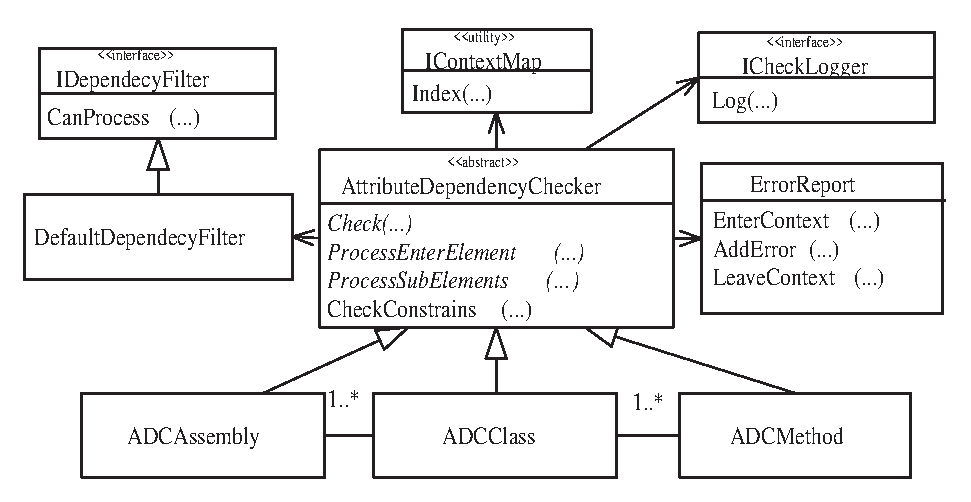
\includegraphics[width=12cm,height=!]{ch04b/implementation2}
	\end{center}
	\caption{The Run-time Attribute Dependency Checker Structure}
	\label{fig:implementation}
\end{figure}

\begin{figure}[ht]
\begin{center}
\begin{minipage}{7cm}
	\begin{scriptsize}
\begin{lstlisting}[numbers=left,language=Java,frame=leftline]{}
Assembly a = ...; // obtain an assembly
ADCAssembly c = new ADCAssembly();
c.Filter = ...;   // set filter
c.Logger = ...;   // set logger
c.Check(a);       // check the assembly
if(c.errors.HasWarnings())
{ // process: c.errors.GetWarnings() ... }
if(c.errors.HasErrors())
{ // process: c.errors.GetErrors() ... }
\end{lstlisting}
  \end{scriptsize}
\end{minipage}
\end{center}
  \caption{Using the Run-time Attribute Dependency Checker in Code}
	\label{fig:using}
 \end{figure}

In order to implement the semantics of the dependency attribute, initially the attribute dependency sets need to be built for every structural element, by processing the element and all its structural children. After the dependency sets are constructed, the dependency constrains of the element can be checked. That is, a post-order transversal of the structural tree is required. A boolean flag in \texttt{Attri\-bute\-De\-pen\-de\-ncy\-Che\-cker} controls whether the inherited attributes of the structural elements are processed or not. 
The actions performed during a call to the \texttt{Check(t)} method (line 5 in \fig{fig:using}), where \texttt{t} is the current program element whose attribute dependencies are being checked for, are illustrated in \fig{fig:seq-diag}. 

\begin{figure}[ht]
	\begin{center}
		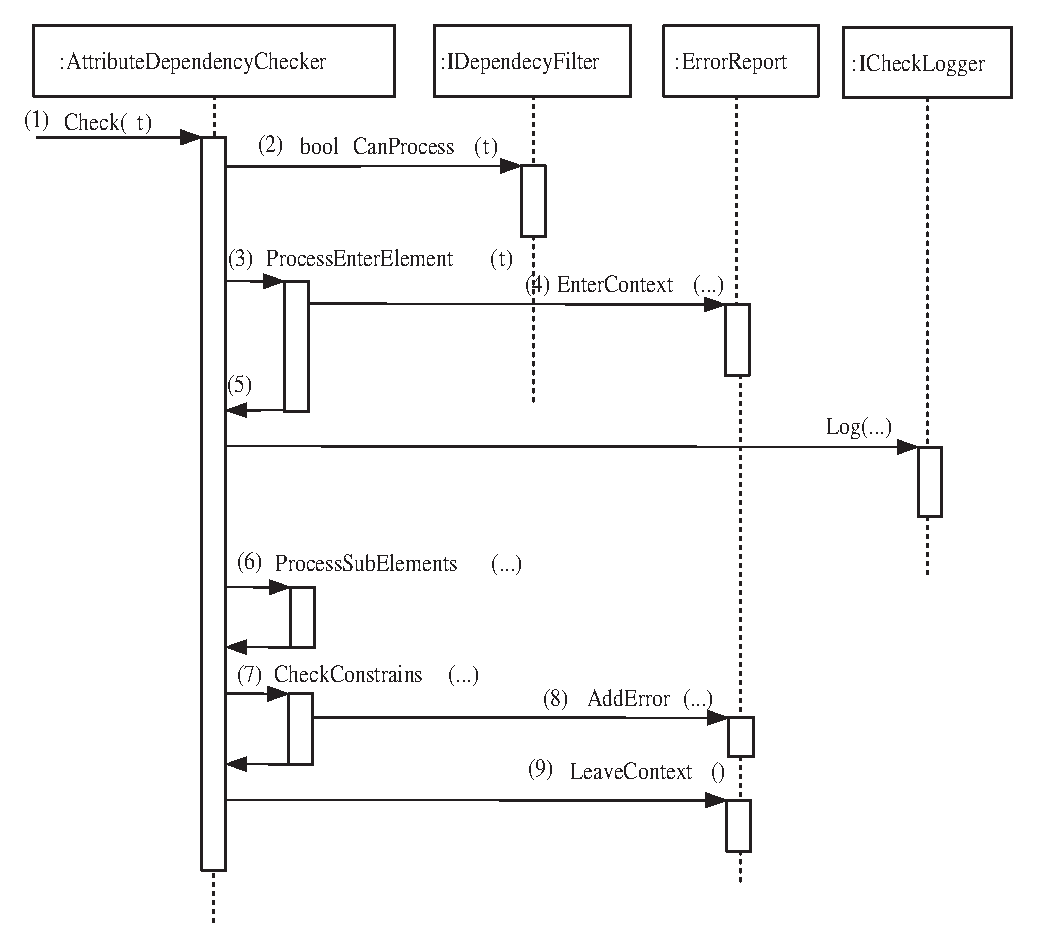
\includegraphics[width=12cm,height=!]{ch04b/seq-diag}
	\end{center}
	\caption{UML Sequential Diagram of \texttt{Check()} Method Call}
	\label{fig:seq-diag}
\end{figure}

First, the filter object is used to check whether the element at hand should be processed (step 2 in \fig{fig:seq-diag}). 
Filters can be used to put arbitrary constraints on the elements that will be processed, e.g., by using pattern matching on names. The \texttt{De\-fault\-De\-pen\-de\-ncyFi\-lter} processes all the elements. 
The ADC command-line tool uses a customized filter called \texttt{Class\-De\-pen\-de\-ncyFi\-lter} derived from \texttt{De\-faultDe\-pen\-de\-ncyFi\-lter} that can restrict checking to a subset of classes, whose names are given in the command-line. More sophisticated filters can be written and used programmatically (line 3 in \fig{fig:using}). Filters can also be used to implement profiling by keeping track of various counters; e.g., \texttt{Class\-De\-pen\-de\-ncyFi\-lter} counts the number of classes and the methods processed.

Next, the call to \texttt{Process\-Enter\-Element()} (step 3) sets the proper \texttt{Error\-Report} context (explained later) in step 4, which is used when processing the sub-elements of the element at hand. The \texttt{Process\-Sub\-Ele\-ments()} method in step 6 calls the \texttt{Check()} method of all sub-elements. As shown in \fig{fig:implementation}, the specific attribute checkers for different meta-elements, e.g., \texttt{ADC\-Assembly} and \texttt{ADCClass}, are derived from \texttt{Attri\-bute\-Depe\-ndency\-Che\-cker} by implementing the abstract methods: \texttt{Check(object t)}, \texttt{Pro\-cess\-EnterEle\-ment(object t)}, and \texttt{Pro\-cess\-Sub\-Ele\-ments(ref Array\-List ctx,\- object t)}.
For illustration, \fig{fig:proc-sub-impl} shows the implementation of the \texttt{Pro\-cess\-Sub\-Ele\-ments} method in \texttt{ADC\-Class}. Only the traversal functionality for finding the sub-elements is part of this method.

\begin{figure}[ht]
\begin{center}
\begin{minipage}{12cm}
	\begin{scriptsize}
\begin{lstlisting}[numbers=left,language=Java,frame=leftline]{}
protected override void ProcessSubElements(ref ArrayList ctx, object t) {
  MethodInfo[] m = ((Type)t).GetMethods(
    BindingFlags.Instance |
    BindingFlags.Public |
    BindingFlags.DeclaredOnly |
    BindingFlags.NonPublic);

  foreach(MethodInfo mi in m) {
    ADCMethod adc = new ADCMethod();
    CopyStateTo(adc);
    adc.InitialContext = ctx;
    adc.Check(mi);
  }
}
\end{lstlisting}
  \end{scriptsize}
\end{minipage}
\end{center}
  \caption{\texttt{ADCClass} Implementation of \texttt{ProcessSubElements} Method}
	\label{fig:proc-sub-impl}
 \end{figure}

The context to be used during the processing of a node and its descendants (the parameter \texttt{ctx} in the signature of \texttt{Pro\-cess\-Sub\-Ele\-ments}) is managed as an \texttt{Array\-List}, similarly to the method call stack frames in a compiler \cite{aho.88}.
A frame in the context array contains the attributes and the dependency attributes of a particular element. As the structural tree is traversed by calling \texttt{Pro\-cess\-Sub\-Ele\-ments}, the dependencies context is filled by passing the \texttt{ctx} object to every processed sub-element. When being processed, an element can modify the dependency information of the context frames of its parents.
%After a sub-element has been processed, its frame is removed (pop up) from the context.
After all sub-elements of a given element are processed, all the required context information is in the context stack frames. This information can be used to check the dependencies of the given element. The dependency meta-attributes of the current attribute are compared with the total dependency attributes for the current frame, using set operations in the \texttt{Check\-Con\-strains()} method (step 7 in \fig{fig:seq-diag}).
 
The \texttt{:Error\-Re\-port} object maintains its own separate context stack (set up in step 4), so that when an error is reported in step 8, the error message can be embedded within the proper structural context. The \texttt{Error\-Re\-port} context is used to report messages in a useful way, as illustrated by the error message:

\begin{scriptsize}
\begin{verbatim}
| Required CLASS attribute missing:
| adctests.CA01Attribute @ adctests->adctests.nunit.TDependencyUtils
\end{verbatim}
\end{scriptsize}

\noindent This error message specifies that the required class attribute \texttt{adc\-tests.CA01\-Attri\-bu\-te} is missing in the class \texttt{adc\-tests.nunit.TDe\-pe\-ndency\-Utils}, which is part of the \texttt{adctests} assembly.
%
By default \texttt{Error\-Re\-port} accumulates the errors, but this behavior can be changed via a switch, so that it will stop the checker execution when an error happens, by throwing a \texttt{ADC\-Excep\-tion}. The \texttt{Error\-Re\-port} contains also functionality to accumulate, or immediately report, the improper usages in code of the parameters passed to the \texttt{De\-pe\-ndency\-Attri\-bu\-te} itself. An example is passing an attribute declared with a class lexical scope, as an argument to a \texttt{Re\-quired\-Me\-thod\-Attri\-bu\-te} property.

Finally, the \texttt{ICheck\-Logger} interface (step 5) enables the programmer to associate a custom output stream logger with the dependency checker (line 4 in \fig{fig:using}). If the logger stream is not \texttt{null}, a hierarchy of the processed elements with details about their attri\-bu\-tes and attri\-bu\-te dependencies is printed in the logger stream. A filter could also be used for custom logging. All objects shown in \fig{fig:seq-diag}, with exception to the  \texttt{:Attri\-bu\-te\-De\-pende\-cyChe\-cker}, are singletons and are passed to the processing of the sub-elements as part of the context. 

The implementation of the class \texttt{Attri\-bu\-te\-De\-pe\-ndency\-Che\-cker} is generic with regard to the implementation of both the \texttt{De\-pe\-ndency\-Attri\-bu\-te} and the meta-model elements. This means that the implementation of the \texttt{Attri\-bu\-te\-De\-pe\-ndency\-Che\-cker} class can be reused with new attributes as well as with other meta-model elements. The \texttt{Attri\-bu\-te\-De\-pe\-ndency\-Che\-cker} achieves this generality by using a combination of the following three techniques:

\begin{itemize}

\item First, all the hierarchy information of the supported meta-model is factored out into two static methods of the \texttt{ICon\-text\-Map} utility class. \texttt{Attri\-bu\-te\-De\-pe\-nden\-cy\-Che\-cker} uses the \texttt{ICon\-text\-Map} to implement a strategy pattern \cite{dpatterns}. By changing the \texttt{ICon\-text\-Map} class, users can change the supported meta-model. Theoretically, the information in the \texttt{ICon\-text\-Map} is enough to check the dependencies, i.e., no specific checker classes for different elements of the meta-model, e.g., \texttt{ADC\-Class} would be needed. However, the .NET Reflection API design is not consistent for traversing the meta-elements hierarchy. Other API-s, e.g., XML DOM \cite{mcl.01}, have a single base interface\footnote{The \texttt{Node} interface in XML DOM.}, from which all elements are derived. .NET Reflection API does not expose a single generic interface for all meta-element types, because the number of meta-elements is limited. This requires that when adding new meta-elements to the ADC library, special classes need to be derived for the new elements. These new classes will contain only code to traverse the sub-elements, as described above (\fig{fig:proc-sub-impl}).

\item Second, given that the structure information of the meta-model is present in the \texttt{De\-penden\-cyAttri\-bute} property names, the reflection inside the \texttt{Check(...)} method is used over the \texttt{De\-pende\-ncyAttri\-bute} properties, to map them to the internal \texttt{ICon\-text\-Map} data. The use of the reflection ensures that if the required / disallowed properties of the \texttt{Depe\-nde\-ncy\-Attri\-bute} class are added or removed, the implementation of the \texttt{Attri\-buteDepen\-dencyChe\-cker} does not need to be changed. Another generic alternative would be to generate the checker code based on the \texttt{Depen\-dency\-Attri\-bute} implementation, but this would require to re-generate and re-compile the \texttt{Attri\-buteDepen\-dencyChe\-cker} class for every different version of the \texttt{Depen\-dency\-Attri\-bute} implementation.

\item Third, the template method pattern \cite{dpatterns} is used to call abstract methods that need to be implemented in the derived classes, such as the \texttt{Proce\-ssSubEle\-ments} method in \fig{fig:proc-sub-impl}, required to traverse the sub-elements. The entire checking functionality is part of the abstract class \texttt{Attri\-buteDe\-pende\-ncyChe\-cker}.

\end{itemize}

The resulting ADC library can be easily extended to support new meta-elements. If a new type of checker for attributes of another meta-element need to be added, then a class from \texttt{Attri\-bu\-te\-De\-pe\-ndency\-Che\-cker} must be derived. The derived class implements the abstract methods discussed above. In addition, the \texttt{ICon\-text\-Map} class needs to be modified to accommodate the hierarchical structural relation of the new element, with regard to the existing elements. 

\section{Related Work}
\label{sec.c4.related}

%Attribute transformations techniques presented in this chapter are specialized for the interpretation of attribute-based DSA required in mobile product-lines. The vertical and horizontal modularization techniques are made possible only by exploring the characteristic of this specific domain and the hardwired language meta-model. The specific modularizations would not have been possible if attribute transformations were addressed from a more generic level.

Attributes are a form of graph labeling \cite{term.rewrite,Plump.95,mens.99}. Attributes make it possible to associate arbitrary semantics with graph nodes of interest, and can be used to drive graph transformations. Considering attributes in a very generic level is not very useful in practice. For example, being able to normalize a series of add / remove / modify operations applied to a graph \cite{mens.99} is an interesting theoretical operation. In the domain of mobile applications considered as a use case in this book, the scenarios that add the same block of code or method, or remove it several times, do not happen. Graph labeling is more interesting when it is specialized for a domain. For example, in \cite{Biggerstaff.ICRS6} tags are used to reduce transformation search space \cite{ptm.03} by serving as transformation hints, in the same way as tags in MDA \cite{mda.frankel} models. The class of graph labels addressed in this book is made of attributes used directly at the programming language level. Attributes are complex graph labels that are specialized using parameters, contain behavior, and could be decorated themselves with other attributes.

Several general-purpose languages, such as .NET \cite{www.dotnet} and Java 1.5 \cite{www.java.attrib.04}, already offer support for attributes. As discussed in \kr{ch03}, these languages offer also GAAST-like means to process the code decorated with attributes. Other non-mainstream approaches also exists \cite{java.explicit.programming,java.attrib4j}. These approaches fall in the category of API-based generators \cite{voelter.generation,generative.00}. The GAAST-level of generality was the starting point for the modularization techniques presented in this chapter. The parsing issues were not addressed on purpose in Tango, to provide flexibility to use any GAAST API, or meta-programming tool discussed in \sr{sec.meta.prog}, e.g., \cite{java.openJava,batory98jts,java.jse,java.epp,java.maya,qdox} to map the AST to the common Tango OO model.

Tango modularization techniques can be seen as domain specialization of graph rewriting systems \cite{term.rewrite,Nagl:96,mens.99}. The changes introduced by an attribute-driven transformer to an annotated class could be seen as a series of primitive operations. Tango supports a hardwired language meta-model with a finite number of elements. This makes it possible to enumerate the edit operations. The approach is similar to implementing graph-based schema evolutions \cite{Banerjee.87}, but specialized for a special set of OO attribute-driven transformers.

Stratego \cite{stratego.01,ptm.03} is a library of strategy operators and traversal primitives to reduce the program transformation costs. Stratego is implemented as a set of reusable transformations primitives that can be used with any language system, given that a suitable parser to map the specific language constructs, to Stratego constructs can be created. The Stratego modules are translated to C code. Stratego organizes transformation operations as series of strategies that work over grammar rules, to support, for example, term rewriting \cite{term.rewrite}. \textit{"A strategy is an operation that transforms a term into another term or fails"} \cite{stratego.01}. A strategy is made up of:
\begin{itemize}
\item \textit{Traversal primitives} that support reusable term traversal techniques. Examples: \textit{all} - all nodes in an expression; \textit{repeat} - an generic iteration strategy to repeat an operation; \textit{bottomup} - does a bottom-up traversal of an expression.
\item \textit{Strategy operators} that allow the combination of strategies. Examples: \textit{sequential composition} - combines a sequence of  traversal primitives; \textit{choice} - selects between two or more traversal primitives. 
\end{itemize}

\noindent The approach presented in Tango is different in two ways from Stratego: (a) the strategies are organized in layers and (b) the strategies are specialized for the entities of each layer.

There are several general-purpose transformation frameworks, e.g., DMS \cite{dms.02}, TXL \cite{txl.04} and ASF+SDF \cite{asfsdf.02}, which can be used to address domain-specific transformations. These general-purpose frameworks have an open meta-model meaning that any specific language can be mapped to them. These tools could also be used to process explicit attributes. However, generic frameworks do not provide declarative specialized rules for every specific domain of interest. Hardwiring the domain, as in Tango, enables abstracting the transformation strategy operations at different levels. 

Tango's vertical attribute modularization bears resemblance to layered context-sensitive graph grammars \cite{Rekers-Schuerr02:97} and multi-stage programming \cite{Taha.1997}. Layered grammars \cite{Rekers-Schuerr02:97} have been used to recognize left-hand side patterns in graphs, and specify an evaluation order for graph rewriting rules. Tango is specialized only for attribute-driven transformers. Multi-stage programming uses special annotations to structure the computation of expressions as multi-stage transformations. Multi-stage programming is driven by the need for optimizations and partial evaluation \cite{jonesetal.93} and uses a predefined set of annotations. Tango can be used to implement arbitrary invasive transformers \cite{java.compost} at source code level, in the top of a GAAST-like language. Tango also supports an arbitrary number of user defined attributes. 

Some transformation approaches generalize the ways a transformer works with an AST-like representation of the program: (a) \textit{Filtering related approaches}, e.g., JPath \cite{extract}, are motivated by XPATH \cite{url.xpath} node query language for XML \cite{skonnardetal.01}. The idea is to be able to define XPATH-like queries over the AST to declaratively select sets of nodes of interest. For example, the query  "\texttt{//class[@name=\-"Class1"]/\-method[@name=\-"Method1"]}" selects and returns all methods named \textit{Method1} found in class named \textit{Class1}. (b) \textit{Mapping related approaches} build upon filtering related approaches and that are motivated by XSLT \cite{xslt} and more recently by MOF Query View and Transformation \cite{mof-qvt-ibm-sub.03} proposals. These approaches define declaratively how to map a set of selected nodes to another set of nodes, enabling this way the generic transformations of one graph to another. These approaches are very general. For example, XML and XPATH are used internally in Tango to implement the specific Tango features on top of them.

The feature-based categorization of MDA transformation approaches presented in \cite{model-approach.03} distinguishes between \textit{model-to-code} and \textit{model-to-model} approaches. Tango is a \textit{code-to-code} transformation framework. Given that the transformation of a marked model to marked code is trivial \see{sec.gaast.map}, the approach can be seen also as \textit{model-to-code}. With regard to the implementation, Tango can be seen as a \textit{template}-like transformer with source-oriented deterministic iterative rules. The categorization in \cite{model-approach.03} is too wide, and many tools could fall into the same category. Tango is unique for its well-structured layers, extensibility of primitive operations, and heavy reliance on inner tags.

Code snippets in Tango are an example of the combination of template and frame-based systems \cite{generative.00,voelter.generation}. Similar approaches include syntactic unit trees \cite{majkut.03} and various template and macro-based approaches \cite{java.epp,java.jse}. Tango code snippets differ from these approaches, because code snippets are restricted to represent only non-structural elements, e.g., a block of code inside a method. Tango code snippets can also be labeled with inner tags and reprocessed later as atomic elements of the AST.

Declaring and checking attribute dependencies is one example of explicitly enforcing architectural principles \cite{minsky.98}. Attributes offer a unified way to express evolution invariants in languages that support explicit annotations, given that any structural entity can be decorated independently of the syntax. This makes attributes attractive for expressing law-governed system evolution rules. Architectural principles that must hold between program entities can be expressed as attribute dependencies between architectural attributes used to decorate program entities. System-wide invariants can be expressed in .NET as \texttt{Asse\-mbly} attributes and system-wide rules can be expressed declarative by using meta-attribute annotations over the architectural attributes.

The meta-attributes approach enables explicit factorization of cross-cuttings concerns in attribute-driven transformers. Meta-attributes make the cross-cuttings concerns definitions declarative and fit well in the paradigm of a GAAST language. Meta-attributes are not well-suited for checking arbitrary program restrictions. Cross-cuttings concerns based on meta-attributes can be factorized using specific tools, e.g., ADC \see{sec:adc} or any generic me\-ta-pro\-gramming tool. There are also generic me\-ta-pro\-gramming tools \cite{www.pmd,www.tj,XIRC} designed to ease enforcing of program rules that cannot be checked directly by the programming language compiler. These tools could be used to implement checking based on attributes directly, or based on meta-attribute factorizations if they can access them. Cross-cuttings concerns could also be factorized with AOP \cite{kiczalesetal.97,Laddad.aop,XIRC,aop.attrib.05} techniques \see{ch2:aop}. Aspect-oriented programming techniques can be also used to enforce architectural decisions. An example how AspectJ \cite{www.aspectjt} can be used to enforce system-wide constrains is given in \cite{shomrat.01}\footnote{There are meta-programs that cannot be expressed as AspectJ programs.}. 

Attribute extension grammars can be used to enforce properties about library components that can not be enforced otherwise with object-oriented systems \cite{hedin.97}. The work has been superseded by language technologies, such as .NET \cite{www.dotnet}, that directly support attributes and offer GAAST-like access to the AST information along with the decorated attributes. The meta-attributes approach enforces rules at a more abstract level, using attributes to define declarative rules that must hold between attributes.

It is also possible to define a central notion of dependency and model any kind of dependency by a Dependency Code Calculus (DCC), based on a computational lambda calculus \cite{abadi99core}. Such a formal abstraction can be interesting for proving properties of dependent system elements, but it must be specialized to a specific domain to be of real usage, yielding different special purpose calculuses \cite{abadi99core}. However, some of the dependency problems mentioned in \cite{abadi99core}, such as slicing calculus, do not map directly into source code program dependencies and cannot be expressed as source code attributes.

\cendsection{Chapter Summary}

The transformations of attribute decorated entities become problematic in a system when the number of attributes and their required interpretation context grows. The attribute-driven transformer implementation is the ultimate source of documentation about the semantics of an attribute or a set of such. It is important that the transformation process is implemented in a well structured and modular way to ease understanding and enhance reuse.

The domain knowledge for attribute-based DSA used to support mobile product-lines is explored to modularize attribute-driven transformers. The overall attribute-based DSA transformation is structured in parts corresponding to the domain assets, which are modeled as attribute families.

To enable declarative composition of the transformer units, inner attributes are used to express the inter-transformation semantics. Inner attributes serve as a uniform composition mechanism for attribute-driven transformers, that treat the inner attributes equivalently to explicit attributes. Inner attributes make the transformer coupling explicit.

The knowledge of semantics of the domain assets is used to define the transformation workflow. The process is partially automated by having the dependencies expressed as \textit{before} or \textit{after} lists. The generated dependency graph can be overwritten manually by using specialized workflow operations to resolve potential conflicts.

The hardwired OO language meta-model addressed by Tango is explored to achieve a vertical modularization of transformer units. The transformation strategy is structured according to the nesting of the structural elements in the language meta-model. This structure is enforced with language constructs. Specific strategy operations optimized for each layer are created to make the transformer implementations more declarative.

The common OO meta-model is isolated inside the transformation framework, from the details of the specific language, by using code snippets. Code snippets are parameterized templates that contain language specific syntax, and are used only inside the member constructors, e.g., the method transformers.

Repetitive cross-cutting attribute-transformation concerns are factored out of individual transformers, and made part of generic tools of the transformation framework. Meta-attributes offer a convenient way to implement a mix-ins structure, used to declaratively express the cross-cutting concerns of attribute-driven transformers.

Attribute dependencies are a cross-cutting attribute-transformation concern that is made declarative by using meta-attributes. A special tool was demonstrated, which extends .NET to declare, and automatically check, attribute dependencies using Reflection over the IL binaries. 

\chapter{MobCon: A Generative \hyphenation{Middleware} Middleware Framework for J2ME}
\label{ch:mobcon}
\label{ch05}
\mquote{There is abundant evidence to show that high buildings make people crazy.}{C. Alexander et al, Four-Story Limit pattern, A Pattern Language: Towns - Buildings - Construction, Oxford University Press, 1977}

\noindent MobCon\footnote{The name \textit{MobCon} stands for \textit{Mobile Container}.} is a framework\footnote{This chapter shares content with reference \cite{cepa.mezini.hicss38}.} \cite{vasian.mobcon.03} for automating cross-cutting concerns of Java 2 Micro Edition (J2ME) - Mobile Information Device Profile (MIDP) \cite{www.j2me} applications. MobCon uses the technology for attribute-based DSA applied to organize product-lines, introduced in this book. MobCon is implemented as a generative framework that organizes the product-line domain assets as container-managed services specialized for the MIDP development.

\begin{figure}[ht]
%\begin{center}
	  \xymatrix{
	  	*+[F]{\txt{Automating MIDP Applications\\\Sr{sec.mc.Intro}}} \ar[r] \ar[d] & *+[F]{\txt{MIDP Programming with MobCon  \\\Sr{sec.mc.prog}}} \ar[d] \\  *+[F]{\txt{Mobile Container Architecture \\\Sr{sec.mc.arch}}}
	 \ar[r] \ar[d]  	 & *+[F]{\txt{Extending MobCon Framework \\\Sr{sec.mc.extend}}} \\  	
	  *+[F]{\txt{Related Work \\\Sr{sec.mc.rel}}} 	  &   \\	  	
	  }
%\end{center}
%	\caption{Chapter Overview}
%	\label{fig:contents}
\end{figure}

The domain of J2ME MIDP applications is presented in \sr{sec.mc.Intro}. To support a low-cost programming model, a GAAST-like representation is implemented for MIDP. The domain variability is expressed by means of attribute families.

\Sr{sec.mc.arch} represents the details of mobile containers and how they can be used to structure the MIDP product-line domain assets. A comparison of mobile containers with server-side enterprise containers is presented.

MIDP programming with MobCon is explained in \sr{sec.mc.prog}. The declarative programming model introduced by MobCon preserves the model of the domain assets in code and results in shorter development time.

\Sr{sec.mc.extend} gives details about the MobCon internals. Knowledge of the  MobCon internals is needed to extend MobCon. The plug-in meta-data and customization of the transformation workflow are explained. Related container approaches are discussed in \sr{sec.mc.rel}.

\section{Automating Cross-Cutting Concerns of J2ME MIDP Applications}
\label{sec.mc.Intro}

% This section addresses MobCon aspects that are essential to this thesis.  %Other technical aspects of MobCon, e.g., parser implementations for the MIDP code and details of the network protocols, that could be interesting \textit{per se} are explained only when necessary to support the concepts presented in the thesis.

%\subsection{Mobile Software Development with Platform Abstractions: J2EE MIDP}
\label{c2sec:mobile}
\label{c2.j2me}

The development of mobile software has been moving from OEM\footnote{Original Equipment Manufacturer.} specific operating systems and API-s, e.g., Palm OS \cite{palm} and Windows CE / Pocket PC \cite{wce.2003,PocketPC}, to nearly standardized frameworks, e.g., Java 2 Micro Edition (J2ME) \cite{www.j2me} and .NET Compact Framework (.NET CF) \cite{dnet.compact}. The latter aim at offering the same API to application developers independent of the underlying operating system found in the mobile device. J2ME and .NET CF offer an abstraction of the device hardware and software and enable for the mobile software to be portable from one device to another.
% This section gives an overview of mobile software development techniques focusing on mobile device applications that run on virtual machines.
%
The success behind frameworks, such as J2ME \cite{www.j2me} and .NET CF \cite{dnet.compact}, results from the current trend to abstract from concrete hardware execution models by means of \textit{virtual machine} models against which \textit{pseudo-code} is generated. The pseudo-code is then run (compiled, interpreted, compiled just-in-time) in a specific virtual machine specialized for a given mobile device.

The virtual machine execution model introduces an abstraction between the real hardware and particular OEM software on the one side, and the application programs on the other side. The virtual machine abstraction is especially handy for mobile software, where the underlying device hardware and software models change rapidly. It becomes the responsibility of the manufacturer to maintain the specific virtual machine for the manufactured devices. The software applications are mostly isolated from such changes, unless the newly provided features need to be used.

\begin{figure}[ht]
	\begin{center}
		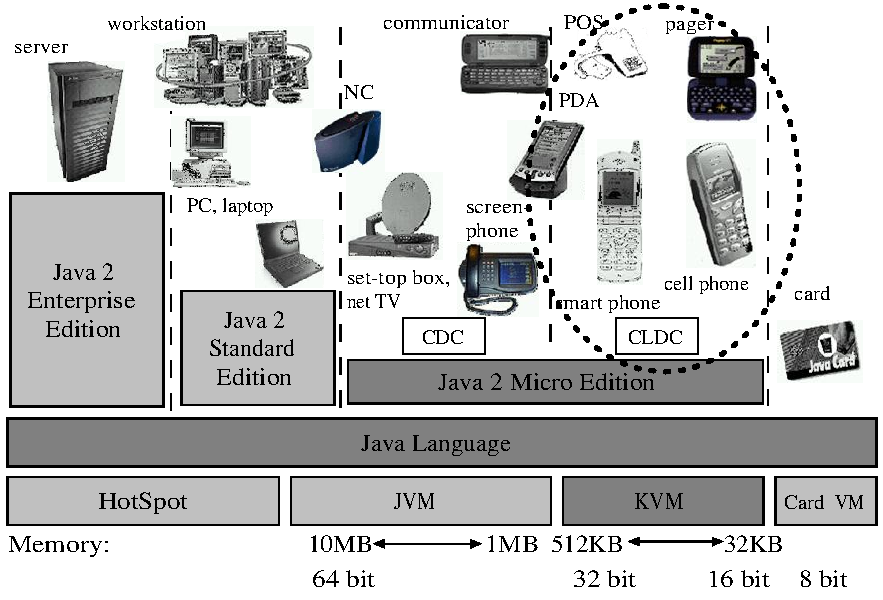
\includegraphics[width=10cm,height=!]{ch02/java}
	\end{center}
	\caption{Java Technologies (Source: http://java.sun.com)}
	\label{fig:java}
\end{figure}

\fig{fig:java} shows the range of the Sun's Java technologies classified according to the targeted devices and hardware technology. Java 2 Micro Edition (J2ME) is the set of Java technologies available for mobile devices. The J2ME technology itself is separated into several families that target different sets of mobile and embedded devices. The most powerful mobile and embedded devices are grouped in \textit{Connected Device Configuration} (CDC) family. The CDC set of devices includes embedded software into TV-Sets, satellite receivers, home video / DVD player devices, powerful PDAs, etc. These devices have enough CPU / RAM resources, power supply sources, and often, constant network connectivity. Standards such as \textit{Open Services Gateway Initiative} (OSGi) \cite{www.osgis}, implemented as \textit{Java Embedded Server} by Sun, target CDC devices that could run some form of the usual Java runtime\footnote{JDK 1.2.}. Scaled down versions of the Java runtime, such as, \textit{Personal Java} profile, could also be used on some of the CDC devices.

Of special interest for this chapter are the devices belonging to \textit{Connected Limited Device Configuration} (CLDC) family. The CLDC family is well supported by Sun and several mobile device hardware vendors \cite{www.j2me.vendors,j2me.2005}. Devices in the CLDC family include, for example, small PDA-s and cellular phones. While PDA-like mobile devices are becoming more and more powerful, the CLDC family will continue to remain in focus as a representative of portable mobile devices. CLDC compatible devices expose many properties usually associated with mobile devices, e.g., limited processing resources compared to other contemporary devices, limited battery life, and sporadic network connections. The CLDC specification is made up of \textit{Mobile Information Device Profile} (MIDP) \cite{www.midp-ota}, whose technology stack is shown in \fig{fig:midp}. MIDP relies on the CLDC virtual machine standard, whose back-end is specialized for the OEM operating system in each device model. The MIDP applications can use the MIDP API-s only and be portable in any CLDC device. Alternatively, MIDP applications can also rely on OEM specific code and be partially portable.

\subsection{The Domain: Automating J2ME MIDP Applications}

The domain addressed in MobCon is that of J2ME MIDP 2.0 \cite{www.midp-ota} applications. J2ME is intended to make programming uniform and simple for mobile devices, following the same goals as Java technology for desktop and enterprise computing \cite{pervasive.java.02}. The MIDP programming model \cite{www.nokia.ep} is based on a very stripped down version of Java. MIDP has a simple language run-time, a simple threading model, and no reflection. The collections and utility libraries are limited to basic types (\texttt{Hashtable}, \texttt{Stack}, \texttt{Vector}). The input / output libraries contain basic stream support. MIDP also contains a set of specialized packages that target CLDC devices. They deal with GUI creation, supporting the idea of a \texttt{Display}, various other input / output gadgets, and game support. It is also possible to play various types of media, e.g., sound or video.

\begin{figure}[ht]
	\begin{center}
		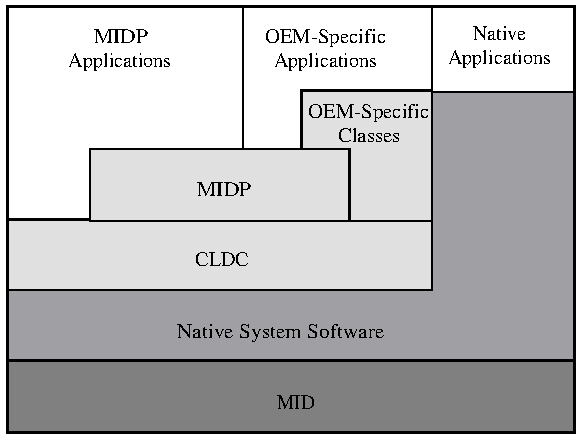
\includegraphics[width=8cm,height=!]{ch02/midp}
	\end{center}
	\caption{MIDP Technology Stack (Source: http://java.sun.com)}
	\label{fig:midp}
\end{figure}

The network communication is supported via a special package for CLDC devices. The basic supported protocols (for MIDP 2.0) include HTTP, HTTPS, UDP, and raw sockets. These protocols are not necessarily supported over TCP/IP. The idea is that any specific device network (packet based) protocol can be used to implement the above protocols and the implementers are free to choose the underlying details. Security is supported via the ability to sign applications and authenticate connections with X.509 certificates. Data persistence is supported via a simple record based model for the local device memory.

A MIDP application is called a \textit{MIDlet}, similarly to a Java applet. A MIDLet should be derived from a specific predefined MIDP class, and should implement a set of required callback methods, e.g., \texttt{startApp()}, that are called by the virtual machine during various phases in the application's life cycle. For an extended and practical discussion about the MIDP programming model the reader is referred to \cite{midp.practical}.

The MIDP technology has proved to be very successful for mobile phones and other small devices, and is supported by many hardware device vendors \cite{lawton.02,www.j2me.vendors,j2me.2005,www.nokia.tp}. There are also good tools and IDE support, and a free reference implementation by Sun. MIDP will be used in this chapter as an underlying technology to demonstrate the concepts represented in this book. 

Despite its simple programming model, MIDP lacks support for modularizing the implementation of \textit{technical concerns}, e.g., data persistence, screen management, session management and security management. These technical concerns \cite{parnas.72} are secondary to what a MIDP application does, but still they must be taken care  explicitly by the developers to get the application running. 
%
When using MIDP, the implementation of secondary concerns cuts across several mobile applications, or even several places within a single application, resulting in duplicated code.
The lack of modularization leads to scattered and tangled code: Not only is the code for technical concerns scattered around several places, it is also tangled with the core functionality. For example, every time the data needs to be saved locally into a mobile device, the \textit{RecordStore} structure that MIDP exposes, needs to be used. The record structure has to be customized manually to match the structure of the data. Similar code is repeated in many places with only very slight differences. The same applies to other concerns, e.g., creating GUI screens and managing the session context.  

The consequence is manifold. First, it makes the development of mobile applications a tedious and error prone task increasing its costs. Furthermore, it is even harder to maintain and further develop such applications, especially in the face of rapidly changing middleware technology for the domain. Given the extreme speed of the domain, it becomes crucial to support off-the-shelf application components that can be reused in a variety of devices. This in turn calls for technology for modularizing technical concerns separately from the application functionality as was explained in \kr{ch02}. 
% it is available for enterprise Java applications, by means of the Enterprise JavaBeans \cite{www.ejb} component model

\subsection{A GAAST-like Representation for MIDP}
\label{mc.gaast}

In \kr{ch03} GAAST-like languages were presented as a prerequisite for introducing low-cost attribute-based DSA to declaratively model the product-line abstractions. The Java dialect supported by MIDP does not support an attribute annotation facility as Java 1.5 does. MIDP also does not support a standard way to access the AST of the parsed MIDP Java code. As the focus in MobCon is in static code transformations, a GAAST-like API for static processing of the MIDP Java code is needed. Adding GAAST-like support to a language is a cheap one-time effort operation. MobCon development was faced with the same problem, to quickly introduce a static GAAST-like representation for the MIDP code. 

The Java dialect of MIDP is similar to Java 1.4. MobCon emulates attributes with JavaDoc \cite{jw-pollac} comments. A special form of JavaDoc comments using an @-sign before the name has been used in several Java 1.4 tools e.g., xDoclet \cite{www.xDoclet} and Attrib4J \cite{java.attrib4j}. When using JavaDoc comments to emulate attributes, no grammar changes need to be introduced in a parser for Java 1.4, apart of the capability to process and preserve the JavaDoc attribute comments. Any tool that parses Java 1.4 could be modified to offer static support for a GAAST-like representation of the source code.

Several third-party generic parsers for Java 1.4 exists, e.g., ANTLR \cite{antlr}, or JavaCC \cite{javacc}. Some specialized Java parsers, e.g., xDoclet \cite{www.xDoclet}, qDox \cite{qdox} have support for processing attributes emulated with JavaDoc comments. Java 1.4 also supports a JavaDoc API that can be used to process JavaDoc comments and could also be used to drive attribute transformations. Unlike full-blown Java code parsers, these tools focus only on parsing  JavaDoc comments and have various limitations in the way they present the Java code. The JavaDoc API, for example, ignores most of the AST information inside methods and cannot be directly used to introduce changes in its model of the Java AST. Other tools, e.g., xDoclet \cite{www.xDoclet} and qDox \cite{qdox}, have similar restrictions. 

\begin{figure}[ht]
	\begin{center}
		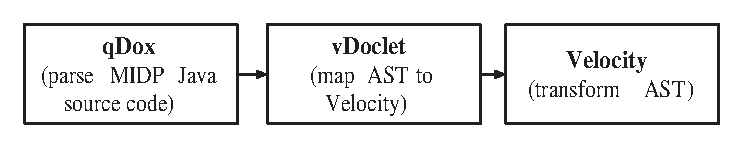
\includegraphics[width=8cm,height=!]{ch05/mobcon-gaast}
	\end{center}
	\caption{MobCon MIDP AST Parsing Tools}
	\label{fig:mc-gaast}
\end{figure}

The qDox \cite{qdox} tool was chosen in MobCon as an underlying tool for creating a GAAST-like representation for MIDP code (\fig{fig:mc-gaast}). There are several, properties that make qDox interesting. As mentioned above, qDox knows how to process JavaDoc style attributes. qDox is also a free open source tool with a very fast parser implementation, which ignores many parts of Java 1.4 syntax. In MobCon, the qDox tool was modified to fully parse MIDP code, that is, to return the method internals as part of the AST and to have support for Java arrays which was not implemented in the original qDox tool. Another very interesting aspect of qDox that motivated its selection in MobCon was the integration of qDox with a tool called vDoclet \cite{vdoclet}. 

The vDoclet tool maps the AST parsed by qDox to a hierarchy of Java objects that can be accessed inside Apache Velocity \cite{velocity} script engine. Apache Velocity is an open source script engine motivated by WebMacro \cite{www.webmacro}, mainly intended for supporting web applications. Using web script engines as meta-programming tools have been explored in many tools, one of the first being Gen\verb@<X>@ \cite{www.genx}. The core of the Velocity is a generic template-like engine that can be used to transform any kind of parameterized source templates. An interesting property of Velocity is that it contains only very basic programming constructs, but allows any Java object to be mapped onto Velocity and accessed directly from the script code. The vDoclet \cite{vdoclet} tool uses this property of Velocity to make the Java AST accessible as native objects in Velocity. The vDoclet tool was also modified in MobCon to reflect the changes that were introduced in qDox. This way, a complete GAAST-like engine was made available in MobCon for transforming the J2ME MIDP applications.

\subsection{Modeling MIDP Attribute Families}


Attribute families were introduced in \sr{attribute.families} as a way to model the variability of the product-line domain assets with attribute-based DSA. MobCon models the generic non-functional MIDP concerns as attribute families. The attributes of the same family are combined with a name space dot-like notation.

\begin{figure}[ht]
	\centering
	\begin{minipage}[b]{5cm}
	\begin{center}	
\begin{footnotesize}
\begin{verbatim}
@src
|- height
|- width
+- form
|  |- label
|  |- firstDisplay
|  ...
|  |- choiceGroup
+- textfield
|  |- label
|  ...
|  |- maxSize
...
\end{verbatim}
\end{footnotesize}
	\end{center}
		\end{minipage}	
	\caption{The MIDP Screen Management Attribute Family}
	\label{mc:scr}

\end{figure}


For example, the attribute family \texttt{@scr}, part of which is shown in \fig{mc:scr}, denotes the screen management concern \see{sec.mobcon.hello}. Inside a family, attributes are distinguished by the family sub-prefix separated by dots. For example, \texttt{@scr.label} denotes the technicalities involved with managing a label gadget within the screen management concern. Many MIDP attributes take arguments that are represented as strings separated by space after the attribute name, e.g., \texttt{@scr.label "First Application"} specifies the text attribute of a label.

End-programmers of the MobCon use the predefined set of MIDP attributes that come with the framework to build mobile applications.  If an attribute is used inside a component (class), MobCon requires that the attribute family name be present to decorate the component itself. The decorated source code is then processed and the required MIDP technical concerns are injected.

\subsection{The MobCon Transformation Engine}
\label{sec.mc.mte}

The \textit{MobCon Transformation Engine} (MTE), illustrated in \fig{fig:mc-mte}, is designed to be a general-purpose transformation framework organized around the modified Java 1.4 parsing tools introduced in \sr{mc.gaast}.

\begin{figure}[ht]
	\begin{center}
		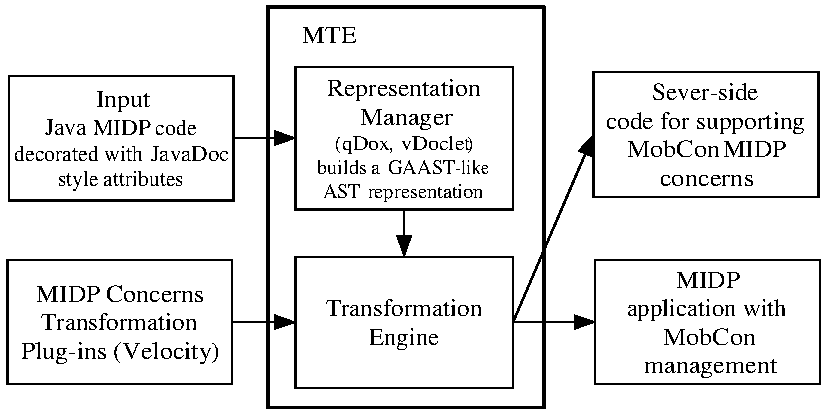
\includegraphics[width=10cm,height=!]{ch05/mte}
	\end{center}
	\caption{MobCon Framework}
	\label{fig:mc-mte}
\end{figure}

The individual MIDP concern transformers are implemented as plug-ins. A plug-in may contain one or more Velocity scripts, Java code, or other resources that describe the plug-in \see{sec.mc.extend}. The MTE contains functionality to properly find plug-in dependencies and manage the transformation workflow \see{sec.mc.wf} by invoking the Java parsing and transformation tools as necessary. Experience with MTE plug-ins was used to develop the Tango attribute-driven transformation framework. Tango and different aspects of building modular attribute-driven transformers processing including those in MTE were discussed in \kr{ch04}.

MobCon relies on the template method pattern \cite{dpatterns} to support well defined extension points \see{sec:ooframeworks}. An abstract class, {\tt AbstractMobApp}, that inherits from MIDP {\tt Midlet} contains the bulk of the generated code. Users do not modify this class directly, since it is modified by the generator each time the attributes in the original source change. Instead, programmers add code to a derived class, {\tt MobApp}, which is called by the abstract class. 
The  template method pattern is useful for generative frameworks \cite{voelter.generation}. It allows programmers to extend the generated code in a modular way without editing it directly.

\subsection{The Mobile Container Architecture}
\label{sec.mc.arch}

\Sr{c2.container.domain} motivated the usage of the software containers as an architectural abstraction to organize the domain assets in software product-lines. \Sr{c2.mobile.container} explained the need to specialize the container concept to address the MIDP domain concerns. One or more mobile client applications run on a mobile device and could connect with server-side services as illustrated in the case (a) of \fig{fig:mob-con-arch}. The server-side part contains functionality that is common to server all clients and functionality specialized for mobile clients, shown by the gray box part in the case (a) of \fig{fig:mob-con-arch}. This specialized client functionality can be factored out from the server part into a separate server-side component known as \textit{adaptive proxy} \cite{fox98adapting}, as in the case (b) of \fig{fig:mob-con-arch}. This separate part is called a \textit{proxy} because it impersonates the server to the mobile clients and vice-versa the mobile clients to the rest of the server (environment) services. It is called an \textit{adaptive proxy} because it does not simply forwards the messages and data from the mobile clients to the server and vice-versa, but also actively modifies the data to adapt them to the specifics of mobile clients. An example of such adaptation is the modification of the resolution of images returned by the server services, to match the resolution required by a mobile device.

\begin{figure}[ht]
	\begin{center}
		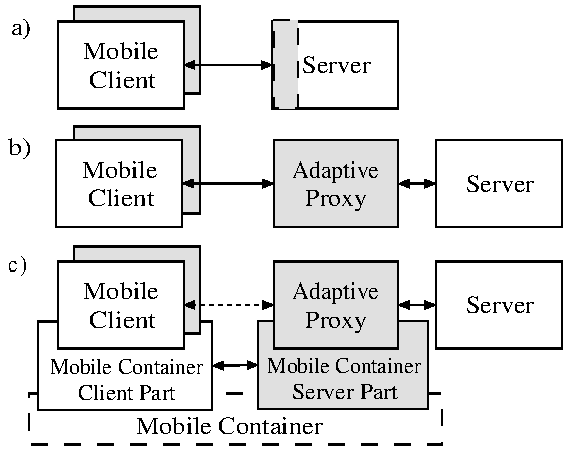
\includegraphics[width=10cm,height=!]{ch05/mc}
	\end{center}
	\caption{The Mobile Container}
	\label{fig:mob-con-arch}
\end{figure}

A mobile container addresses the automation of technical concerns in a mobile application. However, because the functionality of the adaptive proxy part is tightly connected to the functionality of the mobile clients, a mobile container automates both the mobile clients and the adaptive proxy, as in the case (c) of \fig{fig:mob-con-arch}. The mobile client can rely on the container to provide common services specialized for its requirements. In a similar way, in the server-side, the adaptive proxy can make use of the server-part of the mobile container services. The mobile container supported services in both client and server parts are generated and injected based on the requirements of the mobile applications. While a mobile client can still use the server-side services directly, usually it will rely on the mobile container to manage all the communication.

%mob-container
\begin{figure}[ht]
	\begin{center}
		\includegraphics[width=15cm,height=!]{ch05/mobcon}
	\end{center}
	\caption{Mobile Container Components}
	\label{fig:mob-container}
\end{figure}

The conceptual architecture of a \textit{mobile container} is shown in \fig{fig:mob-container}. A mobile container is made of a \textit{client-side} (\textbf{MCCS}\footnote{\textit{Mobile Container Client-Side} part.}) and a \textit{server-side} (\textbf{MCSS}\footnote{\textit{Mobile Container Sever-Side} part.}) part. In the MIDP programming model, the applications cannot share code, including libraries or carry inter-process communication (IPC). This requires to have a MCSS part for every mobile application. It is specialized by generation in MobCon to contain only the functionality needed by the particular application. The MCSS part is instead shared by many mobile clients. It contains generic code in MobCon to identify the clients and fulfill the client-specific requests. The mobile container as a whole manages the communication between the mobile application and the server, and transparently handles the requirements for services by a mobile application. The application specific functionality in both mobile client and the proxy, that is not provided as generic services by the container, is the only code programmed manually by the developers. 

In MobCon, the MIDP transformation plug-ins contain functionality to generate MobCon MCCS code to support the transformed MIDP application, and MCSS code used to support the MobCon concerns in server. The MCSS code must be integrated manually in a server-side application. In MobCon the container is open and extensible. This means that depending on the specific MIDP product-line, developers could add new services to the mobile container needed by server application apart of those already supported by MobCon. This way the mobile container serves as an architectural abstraction \see{c2.container.domain} to organize the MIDP domain concerns in a product-line. This architecture can support at the same time, several families of different domains.

There are more differences between mobile containers and other software (enterprise) containers apart of the explicit separation into two separate physical parts. A mobile container extends from the client device to the server-side. A normal enterprise container works on the server-side and contains some proxy broker code to run on the client. The mobile container does the reverse. The broker-like code is at the server-side. The MCCS part takes care of automation of cross-cutting concerns in a MIDP application running on a mobile device. In an enterprise container, e.g., EJB \cite{ejb21}, the client-side contains only the communication bus and proxy code \cite{server.patterns.02}. The MCCS contains the complete functionality to manage the concerns of MIDP applications. A MIDP application relies on the mobile container to provide the services that map to the required MIDP domain assets. The container manages different aspects of the MIDP application, e.g., the persistence of the mobile application components, and the network communication between the mobile device and the server-side services. Other, more specific domain services, such as image adaptation \see{sec.img.adapt}, are also supported in the same manner as the more generic services by the mobile container \see{c2.container.domain}.

The MCSS part deals with the server-side cross-cutting concerns (CCCs) \cite{parnas.72,kiczalesetal.97}, which are specific for mobile device applications. A mobile device client is different from a desktop client because of the limitations in the processing power, or hardware configuration, e.g., the size of the screen, or the available memory. A mobile device client is neither a thin\footnote{A thin client, here, is an application that contains only the user interface logic and delegates most of the application-functionality processing to the server. A think client does all the data processing itself.} client, because it should be able to work with sporadic network connections, nor it is thick clients since there are usually processing restrictions on the mobile devices. 
The MCSS part addresses mobile device client issues transparently. The interface of the MCSS part to the rest of the server-side services is that of a normal desktop client. The rest of the server-side software in \fig{fig:mob-container} communicates only with the a mobile device client only through the MCSS. The MCSS part contains, thus, more functionality that its symmetrical part in a client of an enterprise container and handles the technical and specific concerns of the adaptive proxy \cite{fox98adapting}.

\section{MIDP Programming with MobCon}
\label{sec.mc.prog}

MobCon is presented to the end-users as a set of attribute-based DSA that support the automation of several technical (and specific) concerns in a product-line for J2ME MIDP applications. The attribute-based DSA modify the semantics of the existing components of a MIDP application. MobCon currently provides MIDP 2.0 support for \textit{data persistence}, \textit{screen management}, \textit{session and context management}, \textit{image adaptation}, \textit{encryption}, and \textit{network communication}. End-users may extend this set of services or modify the existing services \see{sec.mc.extend}. MobCon generates code for the technical MIDP concerns on the client-side (mobile device) and code to be placed on the server-side. The name \textit{MobCon} will be used synonymously with the term \textit{MIDP mobile container} in this section.

A design goal of MobCon is that the attribute decorated code can be used with the manually written parts of the application in a seamless way. The developers can (a) rely on MobCon for the entire application management, or (b) use parts of MobCon for concerns of interests and ignore the others. Developers can use the MobCon generated components or replace them with their own component implementations. MobCon supports an incremental adoption of the MIDP container model inside a specific application. This section presents the MobCon programming model for MIDP applications. First, several MIDP concerns automated by MobCon are presented. Then a complete MIDP application that combines most of the addressed MIDP concerns for a medical X-Ray diagnostics application is explained.

\subsection{Data Persistence}

Any non-trivial MIDP application needs to store data persistently. The non-volatile memory in a MIDP device is organized as a set of record stores managed via the {\tt ja\-vax.mi\-cro\-edi\-tion.rms} package \cite{www.midp}. Each record store is identified by a name unique for a Midlet\footnote{MIDP applications are known as \textit{midlets}, similarly to Java \textit{applets}.}. It contains byte records identified by an integer, the {\tt recordID}. 
%While the {\tt recordID} is incremented when a record is added, the {\tt recordIDs} in a record store may not be consecutive because of record delete operations. 

A MIDP application might need to save data that are too complex to be indexed only by integers. For illustration, consider the \textit{Ga\-me\-Sco\-re} record store example in the documentation of the {\tt ja\-vax.micro\-edi\-tion.rms} package \cite{www.midp}. A \textit{Ga\-me\-Sco\-re} object contains a {\tt player\-Na\-me}, a {\tt score}, and an optional {\tt comment}. Both the {\tt player\-Na\-me} and the {\tt score} fields are used as primary keys. There is no direct way to enable accessing data in a record store for \textit{Ga\-me\-Sco\-re} via arbitrary primary keys. The {\tt ja\-vax.micro\-edi\-tion.rms} package provides support to map arbitrary keys into {\tt recordID}-s by means of enumerating records in a store according to different criteria. The criteria must be coded in a case by case basis for each record store type by implementing two required interfaces: {\tt Re\-cord\-Compa\-ra\-tor} and {\tt Re\-cord\-Fil\-ter}. The {\tt Re\-cord\-Compa\-ra\-tor} defines a partial order over the records in the store, while {\tt Re\-cord\-Fil\-ter} helps to selects certain records.

When using MIDP, a developer must always take care of the store organization details. The store details are intermingled with the application functionality, in the case of the example with the game functionality. This adds significant accidental complexity to the code. This is illustrated by the implementation of a store for the \textit{Ga\-me\-Sco\-re} data which comes with the {\tt ja\-vax.micro\-edi\-tion.rms} package \cite{www.midp} documentation. The code consists in about 216 lines of code of which, as will be shown below (\fig{fig:gamescore}), only about 12\%, belongs to application functionality.  

The increased complexity of the programming model is only one aspect of the problem with a direct approach for implementing the data persistence concern. Other, tightly related issues are maintenance and evolution, which are made more difficult by the lack of the modularity when directly implementing the technical concerns, e.g., data persistence.
Automating the data persistence issues and hiding them from the programmer is highly desirable. Implementing a MIDP store for custom data is a routine operation in a MIDP application and the details are only slightly different from one case to the other.

\begin{figure}[ht]
	\begin{center}
		\includegraphics[width=8cm,height=!]{ch05/dp}
	\end{center}
	\caption{MobCon MIDP Data Persistence Architecture}
	\label{fig:mc.dp}
\end{figure}

MobCon addresses data persistence as a technical concern to be factored out by the container and automates store management. The complete data persistence architecture is shown in \fig{fig:mc.dp} and is supported by two attribute families \texttt{@dbo} and \texttt{@dp}. The \texttt{@dbo} family supports specialized stores for components entities. The \texttt{@dp} family supports data persistence in a shared common store. To illustrate the \texttt{@dbo} entity data persistence, \fig{fig:gamescore} shows the complete code for implementing the \textit{GameScore} example in MobCon using the \texttt{@dbo} attribute family, as well as some sample code of how the \texttt{Ga\-me\-Sco\-re} class can be used. 

\newpage
\begin{figure}[ht]
	\begin{center}
		\begin{minipage}[t]{8cm}
		\begin{scriptsize}
\begin{lstlisting}[numbers=left,language=Java,frame=leftline]{}
/**
 * @dbo
 */
public class GameScore {
    /**
     * @dbo.pk
     * @dbo.min 1
     * @dbo.max 256
     * @dbo.sort asc
     */
    private String playerName;
    
    /**
     * @dbo.pk
     * @dbo.min 0
     * @dbo.max 10000
     * @dbo.sort des
     */
    private int score;
    
    /**
     * @dbo.min 0
     * @dbo.max 512
     */
    private String comment;
}
/**
 * @dbo.use GameScore
 */
class GameApp {
  ...
  public void modifyScore(string userName)  {
    GameScore g = GameScore.retrieve(userName);
    ...
    g.setScore(...);
    ...
    GameScore.store(g);
    ...
  }
}
\end{lstlisting}
		\end{scriptsize}
			\end{minipage}
	\end{center}
	\caption{GameScore Example in MobCon}
\label{fig:gamescore}
\end{figure}


The \texttt{@dbo.pk} attributes in \fig{fig:gamescore} are used to denote the primary key fields. The {\tt @dbo.sort} is used to specify how the records should be sorted according to the corresponding field. This information and the field type are used to automatically generate the {\tt Re\-cord\-Com\-pa\-ra\-tor} implementation. The information provided by the {\tt @dbo.min} and {\tt @dbo.max} attributes is used to generate simple validation rules for primitive types\footnote{For integers, the {\tt @dbo.min} and {\tt @dbo.max} attributes specify the allowed lower and upper bounds, whereas for strings they specify the same bounds for the length.}. In addition, an implementation of the {\tt Re\-cord\-Fil\-ter} interface is generated to enable record matching based on the values of primary key fields. Filtering support also includes queries over records by means of the individual primary key fields.

The MobCon implementation of the class \textit{GameScore} in \fig{fig:gamescore} consists of only 27 lines of code, that is, 8 times less than the pure MIDP implementation\footnote{For details about the generated code see \cite{vasian.mobcon.03}.}. Furthermore, the semantics of  the data persistence are declaratively stated in the MobCon implementation, rather than being buried in complicated imperative code for implementing the comparators. The generative MobCon container frees the programmer from having to deal with data persistence details. The programmer uses declarative attribute-based syntax to express the required functionality and can concentrate on the logic that is peculiar to the application. The MobCon framework handles all the details of the data persistence implementation. The attribute-based variability mechanism can also be easily mapped to a graphical wizard, or a visual modeling tool.

\begin{figure}[ht]
	\begin{center}
		\includegraphics[width=8cm,height=!]{ch05/dpremote}
	\end{center}
	\caption{The \texttt{@dp} Data Store Request Management}
	\label{fig:mc.dp-remote}
\end{figure}

Some mobile applications (or components) might not need a database-like abstraction to persist their data as supported by the \texttt{@dbo} family. A simpler persistence model, in which data is stored as unstructured strings in a hash table structure, i.e., a persistence model more similar to Java serialization, might be good enough. 
%
To support this type of data persistence, MobCon provides the \texttt{@dp} attribute family. Fields annotated with the \texttt{@dp} attribute family are persisted in a shared record store. This common store is also used by MobCon for its internal book-keeping data, e.g., for session and network management. The code needed for performing the data storage is generated by the MobCon framework. 
%
The data of the common store could also be additionally stored remotely on the server, if there is a network connection \see{sec.mc.net}. When the \texttt{@dp} is deployed in a MIDP application, there is a possibility to select between saving all data (a) locally, (b) locally and remotely, or (c) remotely only. These cases correspond to different application scenarios. To explain how MobCon automates remote data storage case consider the logical flowchart of \fig{fig:mc.dp-remote}, which shows how a store data request by a MIDP application is handled by the MCCS part.
 
The deployment case (a) saves all common data locally. In this case the MIDP application stores the data in the mobile device and does not need any remote network connection. The case (b) automatically creates a back-up of the data in server (apart of saving the data locally) when there is a network connection present. When a request for data is made, the local copy is used when no network connection is present. This ensures that the MIDP application can still function reasonably when no network connection is available. The deployment case (c) corresponds to the scenario when the data needs to be saved only remotely, but not locally. This is needed when there is a scarcity of local non-volatile memory in the device, or when the data will be shared and updated by other clients or by the server, and each client needs to operate on the latest copy.

These three scenarios are handled  automatically as part of the \texttt{@dp} deployment. Other scenarios must be currently handled manually. The \texttt{@dp} generated code will take care of establishing the connection to a remote database, if possible, and will perform all the needed actions to persist the common store data for each client on the server-side. Because of the diversity of possibilities for storing data in the server-side (files, different relational databases, XML databases, etc.), MobCon only generates code to manage the store (represented by a \texttt{Tree\-Map}) and serialize data to byte arrays. The developers must add code manually in the proxy to store these data to an appropriate storage organization on the server. In the specific deployment case is known and shared by many applications, then the developers can customize the \texttt{@dp} server-side functionality found in \texttt{Data\-Per\-sis\-ten\-ce\-Trans.ja\-va} file inside the \texttt{@dp} plug-in so that it can be reused by every individual application.

\subsection{Screen Management}
\label{sec.mobcon.hello}

The organization of GUI\footnote{Graphical User Interface.} screens in a mobile application often follows well-defined patterns \cite{www.j2me-ipatterns}. For example, in the \textit{Wizard Dialog} pattern, the user of a mobile application is lead through a series of screens (derived from the class \texttt{Displayable} in MIDP). In this case, it is possible to manage the screen stack automatically, for example, by removing loops, as illustrated in \fig{fig:src.loops}. The screens S2 to S4 in \fig{fig:src.loops} are removed from the stack when S2 is re-shown from screen S4, so pressing the \textit{back} button in screen S2 will show up the screen S1, not S4.

\begin{figure}[ht]
	\begin{center}
$S1 \rightarrow \underline{S2 \rightarrow S3 \rightarrow S4} \rightarrow S2$\\
\textit{remove}
	\end{center}
	\caption{Reducing Loops from the Screen Stack}
	\label{fig:src.loops}
\end{figure}

The MobCon screen management concern takes over the issues related to screen organization and screen stack management. There are attributes in the \texttt{@scr} family to declaratively specify the order of screens, the characteristics of displayed forms, text fields, lists, alerts, and image screens. Common command actions are also taken care by the container implementation of the screen management concern\footnote{More features could be added to this concern in the future, including automatic screen caching and other additional interface gadget combinations.}.

\begin{figure}[ht]
	\begin{center}
	\begin{minipage}{4cm}
		\includegraphics[width=4cm,height=!]{ch05/hellosc1}
	\end{minipage}\hspace{2cm}%
		\begin{minipage}{6.2cm}
		\begin{scriptsize}
\begin{lstlisting}[numbers=left,language=Java,frame=leftline]{}
 /**
  *@scr
  */
 public class MobApp {
   /**
    * @scr.label "Test"
    * @scr.firstDisplay
    * @scr.exitButton
    * @scr.textField textField
    */
   private Form form;
   /**
    * @scr.label "First Application"  
    * @scr.string "Hello World"
    */
   private TextField textField;
 }
\end{lstlisting}
		\end{scriptsize}
			\end{minipage}
	\end{center}
	\caption{MobCon \textit{Hello World} Example Running on a MIDP Emulator}
	\label{fig:hello}
\end{figure}

For an illustration, \fig{fig:hello} shows how a \textit{'Hello World'} MIDP application is programmed using the screen management attributes. The {\tt @scr} attribute attached to the class {\tt MobApp} declares that this class requires the screen management concern.  Only the interface gadget elements are declared as part of the code in the fields {\tt form} and {\tt textField} of the class {\tt MobApp}. Each field element is then decorated with attributes, that declare how it relates to the rest of screen elements. The {\tt @scr.firstDisplay} attribute in line 7 denotes the form that will be displayed first. The form will contain also an 'Exit' button (line 8). The properties of the elements, e.g., their labels, are given as specific attribute arguments.

Most of the repetitive code to be written when a MIDP \textit{midlet} is created, e.g., the required {\tt start} and {\tt destroy} methods, as well as details about implementing the GUI, e.g., the code for creating, customizing and composing the GUI elements, is not explicitly present in MobCon applications. This code is automatically generated by the container. This makes the code involving GUI easier to write and allows the programmer to focus on the core functionality. The interested reader can find the complete MobCon generated code for the simple \textit{HelloWorld} example in \apr{ch.hello.example}. Should the MIDP API-s for managing screen change, the end MobCon based application code does not need to be changed. 

\subsection{Session and Context Management}
\label{sec.mb.session}

Session management is needed in MIDP applications when they communicate with a remote server. The session data support stateful network communication at the application level. For thin clients, it is usually server's responsibility to manage the session data. MIDP applications may want to make use of the possibility to have access to the server session to store their own session data. Related to session management is execution context management, that is, identifying the right mobile device application related to the session data. 

\begin{figure}[ht]
	\begin{center}
		\begin{minipage}[t]{5cm}
		\begin{scriptsize}
\begin{lstlisting}[numbers=left,language=Java,frame=leftline]{}
/**
 ...
 * @ses
 * @ses.rememberLastDisplay
 * @ses.id getMobileID()
 * @log
 * @log.logCommand
 * @log.logMethod
 * @enc
 */
public class MobRay {
 ...
\end{lstlisting}
		\end{scriptsize}
			\end{minipage}
	\end{center}
	\caption{Using Session, Log, and Encrypt MobCon Attribute Families}
\label{fig:mob.ses}
\end{figure}

In MobCon, the context is implemented as a dictionary using a \texttt{Hash\-ta\-ble}. The application can save any data to the context and retrieve them. The session information is saved partially locally, and partially on the server. The session identifier, \texttt{mo\-bi\-le\-ID}, is a unique 128 bit number. This unique ID is assigned to a MIDP application the first time it connects to the server. The \texttt{mo\-bi\-le\-ID} is saved locally by the container for an application in mobile device. The \texttt{mo\-bi\-le\-ID} is reused when the application is reconnected to the server \see{sec.mc.net}. The \texttt{mo\-bi\-le\-ID} serves also as a kind of application \textit{cookie}, which always identifies a particular device instance of a MIDP application. For the session concern, server-side code is generated that handles MIDP sessions and manages the identification based on the \texttt{mo\-bi\-le\-ID} identifiers.

The \texttt{@ses} attribute should be used to decorate the main application class, as shown in \fig{fig:mob.ses}. Predefined support is provided to remember the last displayed form and the unique mobile device session identifier. The session identifier can be changed using the \texttt{@ses.id} attribute. In the example, the parameter of the \texttt{@ses.id} attribute is a code snippet \texttt{get\-Mo\-bi\-le\-ID()} that return the automatically generated \texttt{mo\-bi\-le\-ID}. The \texttt{get\-Mo\-bi\-le\-ID()} is generated by MobCon when the \texttt{@ses} attribute family is used. In a static generative container, such as MobCon, it is possible to use code snippets as attribute arguments. This feature is explored by MobCon to enable the developers to conveniently specify small units of specialization code. 


\subsection{Image Adaptation}
\label{sec.img.adapt}

Mobile devices have limited capabilities so often data, e.g., images, need to be adapted before they are sent to an application that runs on such a device. Images accessed by a MIDP application via a remote server are adapted on the server to match the resolution and colors required by the mobile device. MobCon automatically handles image adaptation using the adaptive proxy pattern \cite{fox98adapting}. The images are stored in their original quality on the server. The MobCon generates code for the MIDP clients as well as for a proxy image adapter to be placed on the server-side. Currently MobCon handles only the MIDP PNG\footnote{Portable Network Graphics.} format images and transforms them on the server-side using JIMI \cite{www.jimi}.

\begin{figure}[ht]
	\begin{center}
		\begin{minipage}[t]{5cm}
		\begin{scriptsize}
\begin{lstlisting}[numbers=left,language=Java,frame=leftline]{}
/**
 * @img.local
 * @img.name "/xrayLocal.png"
 */
 Image ray;
  
/**
 * @img.name getDbe().getImageName()
 * @img.width 100
 * @img.height 100
 * @img.maxcolors 32
 * @img.maxsize 25000
 */
 Image I_ray;
\end{lstlisting}
		\end{scriptsize}
			\end{minipage}
	\end{center}
	\caption{Using Image Attribute Familiy for Static Image Resources}
\label{fig:mob.img}
\end{figure}

The image resource can be either local (stored on the mobile device), or remote and stored in a server. The MobCon \texttt{@img} family can be used to manage the loaded images. The attributes supported by this family allow either decoration of predefined Image objects as shown in \fig{fig:mob.img}, or enable loading images dynamically, by using an automatically generated (overloaded) method:
%Ima\-ge\- re\-trieve\-Ima\-ge(String
%image\-Na\-me,\- int width,\\   int heigth,
%int\- num\-Co\-lors, int\- max\-Size,\- boo\-lean
%di\-ther).

	\begin{center}
		\begin{minipage}[t]{8cm}
		\begin{scriptsize}
\begin{lstlisting}[numbers=left,language=Java,frame=leftline]{}
Image retrieveImage(String imageName, int width, int heigth,
      int numColors, int maxSize, boolean dither){...}
\end{lstlisting}
		\end{scriptsize}
			\end{minipage}
	\end{center}

\begin{figure}[ht]
	\begin{center}
		\includegraphics[width=10cm,height=!]{ch05/mc-img}
	\end{center}
	\caption{The Image Request Management}
	\label{fig:mc-img}
\end{figure}

The name of the image will be used to check first for local images, and then for remote images. \fig{fig:mc-img} shows how a request for an image is handled (a UML sequence diagram). First the MCCS part checks to see whether the image is local. If this is the case, MCCS returns the image to the MIDP application. If the image resource is not found locally, a remote request for the image is sent to the MCSS part. MCSS relies on the manual code written in proxy to get the image from the server storage medium of application. The image is then modified in MCSS to match the MCSS request parameters and is returned to the MCCS, which in turn returns the image to the MIDP application. The MobCon implementation of this concern currently does not cache the returned images, as this consumes a lot of memory in the device. MobCon leaves it up to the application to cache the image, e.g., using the managed \texttt{@dp} store as required.

\subsection{Data Encryption}

Currently, the encryption support in MobCon works tightly coupled with data persistence. When data is transfered over the network as part of data persistence, encryption functionality is added to it when required. This enables safe data exchange even when the \texttt{https} protocol is not supported by the MIDP implementation. In the future, encryption could be exposed as a separate concern to be used with network messages. Encryption can be activated application wide using the \texttt{@enc} attribute as shown in \fig{fig:mob.ses}.

When the encryption is activated the data persistence generated methods will be modified to encrypt / decrypt the serialized byte arrays based on an internal key, generated based on the 128 bit unique application \texttt{mo\-bi\-le\-ID} \see{sec.mb.session}. The implementation of encryption concern is based on the third-party {\tt Bouncy\-Castle} \cite{www.bc} lightweight cryptography API for MIDP. A symmetric AES stream cipher in the CFB mode is used to encrypt the network session data.  

\subsection{Network Communication}
\label{sec.mc.net}

Network communication is currently not an explicit separate concern in MobCon. Other concerns, e.g., data persistence and image adaptation, rely on networking support from MobCon, because their implementation is split between the client application and the server-side (\fig{fig:mc.net}). The exact detail of networking support in MobCon are not of direct interest for the scope of this book, so they will be only briefly explained. 

MobCon supports a centralized way to send and receive network messages automatically. This keeps the number of network connections minimum in order to save resources. MobCon can forward any container management message to the appropriate component using a single TCP/IP socket connection. Network messages are by default asynchronous, running on their threads. The network messages are fully identified by:
\begin{enumerate}[a.]

\item A unique MobCon container instance ID (\texttt{mobileID}) in the device corresponding to a MIDP application. This number is used to identify mobile clients and the MCCS requests in the MCSS part, which deals with more than one client at a time \see{sec.mb.session}.

\item A domain asset plug-in ID that is unique for a given domain. That is, each MIDP concern plug-in has a unique ID. This number is used by the MCCS part to identify the concern's plug-in implementation that issues a message. Different concerns define different message subsets, to request different operations from the MCSS. The message subsets of a concern are further identified by the following two numbers.

\item A plug-in instance ID, that is unique for an application instance of the concern, and allows identifying (if needed) the exact component instance that uses the concern.

\item A plug-in dependent operation code, that can be used to carry out commands between the MCCS and the MCSS parts of the container. This code is implementation specific, and is used to specify the meaning of a network message, e.g., whether it is a data store or a data retrieve request.
\end{enumerate}

\begin{figure}[ht]
	\begin{center}
		\includegraphics[width=8cm,height=!]{ch05/net}
	\end{center}
	\caption{MobCon Managed MIDP Network Communication}
	\label{fig:mc.net}
\end{figure}

\subsection{Traceability}
\label{sec.mc.trace}

MobCon supports traceability in the same way as discussed in \sr{sec.tango.trace}. Traceability is implemented by a special attribute family \texttt{@log}, that can be used as shown in \fig{fig:mob.ses}. The \texttt{@log} attribute family supports the execution traceability. The execution log lists all MobCon transformers that have changed a given method at run-time as shown in \fig{fig:mobray}. The execution log functionality is implemented as just another MIDP plug-in in MobCon.

\subsection{Case-Study: The \textit{MobRay} Application}
\label{sec.x-ray}

To demonstrate the usefulness of the MobCon framework for the J2ME MIDP applications, a complete use-case application called \textit{MobRay} is implemented. MobRay is based on a ubiquitous X-Ray medical diagnostics scenario \cite{www.xray}. In this scenario, a remotely located hospital uploads X-Ray pictures of patients on its web server and registered doctors use PDA-like devices that run MIDP to review images remotely. Doctors send back to the hospital server their diagnostic comments for the reviewed X-Ray images. The MobRay application was chosen because its implementation demonstrates almost all concerns currently supported by MobCon.

\begin{figure}[ht]
	\begin{center}
		\includegraphics[width=12cm,height=!]{ch05/mobray-struct}
	\end{center}
	\caption{MobRay Application Organization}
	\label{fig:mobray-struct}
\end{figure}

The high-level architecture of the MobRay application and its MIDP concerns are shown in \fig{fig:mobray-struct}. The server-side part of this demo application is implemented using a HSQL database \cite{www.hsql} with a simple command-line interface to allow uploading and editing of patient records. The mobile client-side of the application is developed using MobCon. The client-side contains functionality to connect to the server, to authenticate the doctor and to retrieve the x-ray list to be diagnosed. The x-ray patients lists could then be used to review and send comments on selected x-ray images. The MobCon code for the server-side is placed on a folder called \texttt{server} inside the output folder generated for the MIDP application.
%
The entire client side of the application consists of about 300 lines of MobCon source code (including comments), which then results in more than 1500 lines of code (1:5 ratio) in the generated application. Only the application functionality is explicitly coded. All the named concerns in the boxes of \fig{fig:mobray-struct} are handled by the code generated by the framework. 
%Adding more functionality would be possible but it would not demonstrate anything else about MobCon.

\begin{figure}[ht]
	\begin{center}
	\begin{minipage}{4cm}
		\includegraphics[width=4cm,height=!]{ch05/mobray1}
	\end{minipage}\hspace{0.5cm}%
	\begin{minipage}{8cm}
	\begin{tiny}
	\begin{verbatim}
 mobcon.message.MessageHandler: Getting message from server
 METHOD:  commandAction [@ses, @log]
 COMMAND:  'Select' executed in screen 'Choose a Patient'
 METHOD:  choosePatientCG_Action [@log]
 METHOD:  retrieveEntry [@log]
 mobcon.message.MessageHandler: Getting message from server
 METHOD:  setDbe [@dp, @log]
 METHOD:  callF_patient [@scr, @log]
 METHOD:  callSI_patientName [@scr, @log]
 METHOD:  getDbe [@dp, @log]
 METHOD:  callII_ray [@scr, @log]
 METHOD:  getDbe [@dp, @log]
 METHOD:  retrieveImage [@img, @log]
 mobcon.message.MessageHandler: Getting message from server
 METHOD:  callI_ray [@img, @log]
	\end{verbatim}
	\end{tiny}
	\end{minipage}
	\end{center}
	\caption{MobRay Running on a MIDP Emulator and Part of its Execution Log}
	\label{fig:mobray}
\end{figure}

\fig{fig:mobray} shows a screen shot of the MobRay application along with an extract of its execution log generated by applying the MobCon traceability attribute \texttt{@log} \see{sec.mc.trace}. For example, the method \texttt{callF\_pa\-tient} is modified by the screen concern transformer (as it is tagged by \texttt{@scr}). And of course, all methods effected by logging are modified by the traceability concern transformer \texttt{@log} \see{sec.mc.trace}. 

\section{Extending the MobCon Framework}
\label{sec.mc.extend}

The plug-in architecture of MTE \see{sec.mc.mte} enables several types of extensions: (a) the existing plug-ins can be extended with more services for the MIDP assets they manage, (b) the existing plug-ins can be fully replaced with new MIDP plug-ins, or new plug-ins for new MIDP assets could be added, (c) an entirely new set of plug-ins to support a container for a new domain based on Java 1.4 can be introduced. In all the cases, the domain assets are modeled as attribute-based DSA, which removes the need to modify the grammar of the original language. In order to apply successfully the attribute-based DSA and to be able to extend MobCon the transformation details need to be understood. The transformation workflow should be chosen based on the semantics of the domain assets. \Kr{ch04} discussed all these concepts in a generic level based on the Tango framework. This section only explains details specific to the current implementation of the MobCon framework, noting differences between MTE and Tango as necessary. More information can be found in the MobCon documentation \cite{vasian.mobcon.03}.

\subsection{Workflow and Plug-in Metadata}
\label{sec.mc.wf}

A MobCon plug-in is packed as a Java JAR file whose structure is shown in \fig{mc:scr-dirs}. The plug-in JAR file contains, among  other files, a manifest file with custom entries that describes the plug-in meta-data. An example of a manifest file for the session management (\texttt{@ses}) plug-in is shown in \fig{fig:mc.manifest}.

\begin{figure}[ht]
	\centering
	\begin{minipage}[b]{5cm}
	\begin{center}	
\begin{footnotesize}
\begin{verbatim}
<session>
|- MANIFEST.MF
+- <jar>
   |- session.tag
   |- session.vm
   |- ... 
\end{verbatim}
\end{footnotesize}
	\end{center}
		\end{minipage}	
	\caption{The \texttt{@session} Transformer Organization}
	\label{mc:scr-dirs}

\end{figure}

\begin{figure}[ht]
	\begin{center}
	\begin{minipage}[t]{6cm}
		\begin{scriptsize}
		\begin{lstlisting}[numbers=left,language=Java,frame=leftline]{}
Manifest-Version: 1.0

name: Transformer
Transformer-Name: Session
TID: 04
IID: 01
File-Name: session.vm
Tag-File: session.tag
Server-File: SessionTrans

name: Dependencies
Use-Before: 02.01
Use-After: 		
		\end{lstlisting}
		\end{scriptsize}
		\end{minipage}
	\end{center}
	\caption{The \textit{MANIFEST.MF} file for the \textit{Session} Plug-in}
	\label{fig:mc.manifest}
\end{figure}

The manifest file contains several sections identified by the different \texttt{name:} labels in lines 3 and 11 of \fig{fig:mc.manifest}. There is a user friendly transformer name in line 4. The transformation ID (TID) in line 5 identifies the domain concern that the plug-in transformer supports, in this case the session management. The next number, the plug-in instance ID (IID) is the number given to the actual implementation of this plug-in \see{sec.mc.net}. MobCon enables using more than one possible implementation for a given TID in an application, or more often, in different applications. The main Velocity script file of the plug-in transformer is specified in line 8. When the transformer generates also serve-side code (Java SDK 1.4 is used for server-side code), then the line 9 specifies the names for the generated server-side files. The dependencies section, in lines 10 to 13, defines the default plug-in dependencies explained in \sr{sec.workflow}. While user-friendly names can be used, MobCob requires unique identifiers in the form TID.IID to be used in the dependency lists.

\begin{figure}[ht]
	\begin{center}
	\begin{minipage}[t]{6cm}
		\begin{scriptsize}
		\begin{lstlisting}[numbers=left,language=XML,frame=leftline]{}
<flow>
    <group>
        <transformer>
            <name>Screen</name>
            <tid>02</tid>
            <iid>01</iid>    
            <merger>
                <class>MixTemplateExample</class>            
            </merger>
        </transformer>
        <transformer>
            <name>Mix Example</name>
            <tid>07</tid>
            <iid>01</iid>
        </transformer>      
    </group>
...
		\end{lstlisting}
		\end{scriptsize}
		\end{minipage}
	\end{center}
	\caption{MobCon Dependency File}
	\label{fig:mc.dep}
\end{figure}

As explained in \sr{sec.workflow}, the global transformation workflow is calculated automatically in MobCon based on the local plug-in meta-information found in the \textit{MA\-NI\-FEST.MF} file. This frees the developers from having to create the total dependency graph manually. In the MIDP case, the existing plug-in dependencies are specified in their corresponding manifest files. If a new plug-in is added or an existing plug-in is modified or replaced, the plug-in manifest file must be edited to reflect the new order. MobCon supports also an application specific order, where each application can override the workflow order by modifying the \texttt{lib$\backslash$plugins$\backslash$de\-pend.xml} dependency file generated by MobCon inside the application directory. For example, the dependency file of \fig{fig:mc.dep} has been modified to support a custom combination of the output of the \textit{Screen} transformer (line 4) and a custom \textit{Mix Example} transformer (line 12), by using a custom mixer \texttt{Mix\-Tem\-pla\-te\-Exa\-mple} transformer (line 8). A mixer transformer must implement the \texttt{Mix\-Tem\-pla\-te} interface of \fig{fig:mix}. \Kr{ch04} discussed how this concept is generalized in Tango to mix an arbitrary number of classes at the same time.

\begin{figure}[ht]
\begin{center}
\begin{minipage}{12cm}
\begin{scriptsize}
\begin{lstlisting}[numbers=left,language=Java,frame=leftline]{}
public interface MixTemplate {
  public ClassTemplate 
     mixClasses(ClassTemplate ct1, ClassTemplate ct2);
  public MethodTemplate 
     mixMethods(MethodTemplate mt1, MethodTemplate mt2);
}	
\end{lstlisting}
\end{scriptsize}
\end{minipage}
\end{center}
\caption{MobCon MixTemplate Interface}
\label{fig:mix}
\end{figure}

Apart of the dependency meta-data a plug-in file contains also a tag dictionary file (\texttt{.tag}). The tag dictionary is a Java property file that maps the attribute names used in source code to those used by the plug-in internally. This allows developers to customize the attribute names used in code. For example, instead of \texttt{@dp} they could use \texttt{@da\-ta\-Per\-si\-sten\-ce} in code. The plug-in implementation treats the attribute names as string resources: \texttt{\$class.\-get\-Tag(\$tag\-Dic.\-get\-Tag("dp"))}. The trace log will use whatever name the user choses for the attributes.

\subsection{Transformation Details}

MobCon plug-ins use the Apache Velocity \cite{velocity} script engine to manipulate the code. The default mode for the Velocity engine is to output text using the Java \texttt{System.out} object. The MTE modifies the Velocity initialization not to output code directly. Instead, MobCon makes accessible for modification to the Velocity scripts, a set of GAAST-like class template API (CT-API) as explained in \sr{sec.ast.tango}. Working with the CT-API facilitates many aspects of the transformer implementation, that would need to be expressed as text Velocity templates otherwise. The vertical attribute-driven transformer modularization explained in \sr{sec.tango.layers} is not supported in MobCon. For an example of how a transformation can be implemented in MobCon, consider the attribute-decorated code of \fig{fig:mc.code}.

\begin{figure}[ht]
	\begin{center}
	\begin{minipage}[t]{6cm}
		\begin{scriptsize}
		\begin{lstlisting}[numbers=left,language=Java,frame=leftline]{}
 /**
  *@scr
  *@dp
  */
  public class Test{
  . . .
 /**
  * @dp.access
  * @scr.store
  */
  private String id;
		\end{lstlisting}
		\end{scriptsize}
		\end{minipage}
	\end{center}
	\caption{Example MIDP Input Code}
	\label{fig:mc.code}
\end{figure}

\fig{fig:mc.code.vs} shows a part of a transformer implemented in Velocity that processes the \texttt{dp.access} tag in \fig{fig:mc.code}, referred by the name \textit{"accessible"} in the tag dictionary (line 3). A Velocity macro \texttt{dp\_\-meth\_\-get} (lines 9, 16) is used to generate the code in line 5. Inside the macro, a class template object that represents a method is created and mapped as a Velocity object (called a \textit{bean}) by using the vDoclet tool (line 10 in \fig{fig:mc.code.vs}). The method template object is then modified by the macro to customize it to model an accessor method. 

\begin{figure}[ht]
	\begin{center}
	\begin{minipage}[t]{10cm}
		\begin{scriptsize}
		\begin{lstlisting}[numbers=left,language=Java,frame=leftline,showstringspaces=false]{}
#foreach ($field in $class.fields)
  #set($tag = false)
  #set($tag = $field.getTag($tagDic.getTag("accessible")))
  #if ($tag)
   #dp_meth_get($field.type $field.name)
  #end
. . .

#macro(dp_meth_get $type $name)
 #set($MT = $vdoclet.makeBean("mobcon.ct.MethodTemplate"))
 $MT.setAccess("public")
 $MT.setType("$type")
 $MT.setName("get$StringUtils.capitalizeFirstLetter($name)")
 $MT.addEnd("return $name;")
 $CT.addMethod($MT, $tagDic.getPrefix())
#end
		\end{lstlisting}
		\end{scriptsize}
		\end{minipage}
	\end{center}
	\caption{Example Velocity Script for Processing \fig{fig:mc.code}}
	\label{fig:mc.code.vs}
\end{figure}

\noindent The generated code for the accessor method looks as in \fig{fig:mc.code.vs.out}, where a method named \texttt{get\-Id()} is generated. \Kr{ch04} discussed how attribute-based transformers can be further modularized to scale the transformation.

\begin{figure}[ht]
	\begin{center}
	\begin{minipage}[t]{5cm}
		\begin{scriptsize}
\begin{lstlisting}[numbers=left,language=Java,frame=leftline,showstringspaces=false]{}
. . .
  public String getId(){
    return id;
  }
. . .
		\end{lstlisting}
		\end{scriptsize}
		\end{minipage}
	\end{center}
	\caption{Example Output Code for Example of \fig{fig:mc.code}}
	\label{fig:mc.code.vs.out}
\end{figure}

\section{Related Work}
\label{sec.mc.rel}

\Sr{sec.c2.ejb} discussed the J2EE containers and explained that EJB \cite{ejb30} is moving toward a simpler programing model based on attributes. The motivation to use attributes in EJB is not to support a low-cost DSA mechanism. Rather, a predefined specific set of attribute-based DSA is used as a clear and uniform way to support the EJB programming model for enterprise containers. The current version of the latest EJB specification is not fully-completed and leaves the discussion open for feedback in some places, on what is the best way to support a concern, or how to express it better with attributes. MobCon is an open attribute-driven framework for supporting arbitrary attribute-based containers. MobCon is specialized with a set of plug-ins for MIDP applications. The set of attributes that can be used to support a product-line is left open and MobCon enables experimentation. The transformation workflow is customizable and can be modified on a per application basis. The source code parsing engine of MobCon supports a Java 1.4 compatible syntax, similar to the one found in MIDP and has not support for Java 1.5 style annotations\footnote{The AST representation manager could be replaced, if needed, in MonCon to enable Java 1.5 support. The new AST needs to be mapped similarly to vDoclet \cite{vdoclet} tool. These issues are outside the focus of this book. The current MIDP Java dialect syntax is very similar to the Java 1.4.}.

The SmallComponents \cite{www.smallcomps} approach is based on generative techniques and visual modeling to introduce a logical container abstraction. SmallComponents address embedded systems, where the size of the middleware must be optimized with respect to specific application needs. To achieve this goal, an adaptable container abstraction is used as a replacement for the middleware itself. SmallComponents is based on graphical domain-specific languages (UML), rather than on attributes. The SmallComponents approach addresses embedded and real-time systems, where generative approaches are superior to other code abstraction techniques. In MobCon, the container abstraction is not seen as a replacement for the mobile middleware. It rather augments the MIDP middleware with convenient software abstractions to make the MIDP applications easier to develop and maintain. Attributes support a modeling-like view, directly at the source level \see{sec:var.dsa}.

There are many source-to-source transformation and meta-programming approaches and frameworks available \cite{generative.00}. The MobCon transformer framework is specialized for building attribute-driven source code transformers, which may need to be maintained often, to reflect changes in the underlying middleware. Unlike other Velocity-based \cite{velocity} transformers \cite{www.velocity.powered,www.AndroMDA}, MobCon transformers do not use Velocity directly to output code, but rather work on the specialized GAAST-like API \seec{ch03}. This makes it easier to support code generation in the case of cascaded transformers. The effects of attribute-driven transformation and their relation with other transformation approaches were discussed in \kr{ch04}.

Adaptive proxies \cite{fox96adapting,fox98adapting} enable transparent access of server-side services from a mobile client. They stand between the server-side application and a mobile client application, and dynamically adapt the server data requested by the mobile client in order to fit to the capabilities of the mobile client device. The adaptive proxy can reside in the same machine as other server-side services, or in a separate machine. 
MobCon automates the technical concerns of the adaptive proxy related to the mobile application. The server-side part of a mobile container transforms the data to prepare them for the mobile device. MobCon generates the server-side part based on the requirements for the container concerns support in the client-side part. These services are used then by the adaptive proxy functionality.

Aspect-oriented programming (AOP) \cite{kiczalesetal.97} techniques discussed in \sr{ch2:aop} can also be used to support attribute-driven transformations \cite{aop.attrib.05}, and to achieve independence from specific middleware \cite{aop.middleware.03}. AOP tools, e.g., AspectJ \cite{Laddad.aop, www.aspectjt} can be used in two ways to support transformations enabled by MobCon. (a) AOP-style factorizations based on the description of the component joinpoints as pointcuts (implicit hooks \cite{java.compost}) can be used. This is the only available technique in AspectJ before the support for Java 1.5 annotations. This indirect style of programming requires redefining the pointcuts for every component that needs container support, in every specific application, in order to match the advice code. (b) AOP tools can be used to work upon attributes (explicit hooks \cite{java.compost}) as a generic meta-programming engine \see{sec.aop.dsa}. AOP techniques require also some form of run-time support (added statically by AspectJ) to support the pointcut context management. This infrastructure would be appended to the infrastructure code required by the mobile container. The duplicated infrastructure would result in more overhead than with other meta-programing techniques that maintain the node selection context explicitly during the transformation.

AOP techniques could be also supported completely at run-time with additional run-time support. In \cite{aop.da.02} dynamic AOP techniques are used to implement context adaptable sockets. In \cite{spont.container} \textit{spontaneous containers}, based on dynamic AOP, are used along with Jini \cite{www.sunjini} to adapt mobile applications to several environment services. These approaches support for dynamic services. Dynamic AOP techniques are too heavy for MIDP applications and require a more powerful class of devices. For example, MIDP currently does not support programmable code downloading and has no reflection capabilities\footnote{Therefore, Jini \cite{www.sunjini} cannot be used.}, which makes such techniques not applicable. For this reason, the MobCon approach presented here deals only with static transformations of the J2ME MIDP 2.0 applications.

\cendsection{Chapter Summary}

MobCon is a framework for automating technical concerns of MIDP 2.0 applications built upon the concepts introduced in this book. J2ME MIDP applications exhibit repeated cross-cutting functionality that can be factored out from one or more applications. This common functionality can be parameterized and made part of  product-line to support MIDP applications. 

It is preferable to express the MIDP domain assets declaratively in source code. The programmers concentrate on the specific application functionality and express the cross-cutting concerns declaratively. Attribute-based DSA provide a low-cost mechanism for supporting a customizable declarative programming model. A GAAST-like representation of the MIDP Java source is realized based on several open-source tools. These tools allow manipulation of JavaDoc-like decorated source code.

MobCon's programming model is based on the decoration of program entities with attributes. The variability of the technical MIDP concerns is modeled as attribute families. Each family is specialized for a given concern, and contains nested levels of sub-families to express different aspects of the variability. Finally, attribute arguments are used to parameterize the attribute families.
%
The MobCon Transformation Engine (MTE) is organized around the attribute families and employs the different transformation units as plug-ins. MTE contains functionality to drive the transformation workflow based on the plug-in dependencies. The template method pattern is used to separate the generated and manually entered code.

Mobile containers are a special kind of client container specialized to automate the concerns of product-lines for mobile applications. A mobile container automates not only the software running in the client mobile device, but also the related part of software into the server-side. Mobile containers offer an architectural abstraction to organize the domain assets of MIDP product-lines.

Several attribute sets are predefined and automate concerns related to J2ME MIDP, e.g., the persistence of data in the mobile device or across the network. The implemented concerns were selected to be representative of common MIDP tasks, which show up repetitively in many MIDP applications. A case study based on an application for medical X-Ray diagnostics was shown. The addressed MIDP concerns are injected automatically into the X-Ray application, resulting in less code, focusing only to the specific functionality.

The concerns currently addressed by MobCon are by no means a complete set covering every possible MIDP application. The MobCon attribute-driven transformation engine is extensible and allows new plug-ins to be defined and integrated into a container. Plug-ins represent one or more transformers specialized for a specific concern. New plug-ins could add more MIDP services, or provide support for a totally different domain. The generative framework itself is written in Java and is independent of the plug-ins functionality. The transformation control flow is determined based on the declared plug-in workflow preferences, and can be overwritten manually for specific cases.

 
%Some MIDP applications such as games require hand-made optimizations customized to a particular solution. Even general applications can use some of these optimization usually based on compression techniques, such as those mentioned in \cite{optim.midp.02}. In \cite{cepa.netz} we have investigated run-time decompression of .NET assemblies. In the future, such optimizations cloud be made part of the MobCon framework concerns.

\chapter{Summary and Outlook}
\label{ch06}
%\mquote{The terminology is not as important as the concepts. That having been said, you might encounter different sets of terms in other places and should be able to translate between them.}{P. Clements, L. Northrop, Software Product Lines, Addison Wesley, 2002}
%\mquote{For developers writing programs for devices other than the Pocket PC, our samples should run with few if any changes.}{P. Yao, D. Durant, .NET Compact Framework Programming with C\#, Addison Wesley, 2004}
%\mquote{Your quote here.}{B. Stroustrup, The C++ Programming Language, Third Edition, Addison-Wesley, 1997}
%\mquote{It seems in the nature of individuals and organizations to attempt projects that are at the limits of their ability.\\There is no "one right way" to design and build all systems.\\..., we must plan for a series of successes.}{B. Stroustrup, The C++ Programming Language, Third Edition, Addison-Wesley, 1997}
\mquote{I would have made the book shorter, but I did not have any more time.}{E. H. Connell, Elements of Abstract and Linear Algebra, 1999}

\section{Summary}

This book has been concerned with the problem of finding better and faster ways to automate and reuse software in mobile device applications\footnote{Mobile applications, for short.}. The focus has been in (a) developing easy to implement techniques for organizing the common domain functionality in mobile product-lines that (b) enable declarative reuse of the domain functionality in mobile applications. The problem has been addressed (\fig{fig:ac-pl}): (1) by introducing attribute-based DSA supported by GAAST-enabled languages, (2) by having a structured way to interpret attributes with modularized attribute-driven transformers and finally, and (3) by using a software container abstraction to organize the domain assets of mobile application product-lines.

\begin{figure}[ht]
	\begin{center}
		\includegraphics[width=9cm,height=!]{ch06/summary}
	\end{center}
	\caption{Attribute-Supported Container-Based Product-Lines}
	\label{fig:ac-pl}
\end{figure}

After an introduction to the main topics in \kr{ch01}, \textbf{\kr{ch02}} motivated product-lines support for the development of mobile applications and presented mechanisms for implementing mobile product-lines. \Kr{ch02} proposed to organize mobile product-lines with mobile containers, and to support such containers with DSA at the source code level.

\begin{itemize}

\item Automated product-lines are needed to support mobile applications and reuse the common functionality. The mobile product-lines factor out the common functionality of a family of applications and inject the common functionality transparently into a specific application. Automation helps to deal with the cross-cutting nature of the common functionality that is present in more than one application.

\item There are several variability mechanisms for supporting product-lines. Declarative domain-specific abstractions (DSA) supported at the programming language level help to make the domain architecture explicit and to preserve the domain model in the source code. DSA blur the distinction between a modeling phase and the coding phase, and offer support for the traceability of domain concerns in specific applications.

\item A software container serves as an architectural abstraction to organize the domain assets. Containers are known from the domain of server-side enterprise applications. When combined with attribute-based DSA \seec{ch03}, the container offers an architectural abstraction to connect the implementation of the domain assets with the declarative attribute constructs in code.

\item There are many ways to implement containers. Invasive generative containers are better suited for mobile product-lines compared to non-invasive techniques. Invasive containers supported by declarative domain-specific abstractions (DSA) offer more automation and could introduce easy domain-specific optimizations.

\item Aspect-oriented programming (AOP) engines could be used as generic invasive frameworks to implement attribute-driven transformations. Specialized transformation engines are, however, preferable for specific domains. The specifics of attribute-based DSA are utilized to create specialized attribute-driven transformers. AOP and DSA can coexists and complement each-other \see{sec.aop.dsa}. DSA support an explicit programming model and enable vertical automation. AOP-style modularization can be applied over the existing DSA language constructs. 

\end{itemize}

\noindent \textbf{\Kr{ch03}} focused on the aspects of attribute-enabled languages and the effects of \textit{attribute enabled programming} (AEP) in the software development process. GAAST was introduced as a common API of an extensible language workbench, intended to support attribute-based DSA. Several aspects of using attribute-enabled languages in the software development process were investigated.

\begin{itemize}

\item Attribute-based DSA decrease the cost of introducing custom DSA in a language, making attributes preferable for supporting iterative product-lines. Attributes expose a uniform programming model and do not require grammar modifications. Attribute-based DSA selectively customizes the semantics of existing components or language constructs.

\item Domain variability is modeled as attribute families. Each attribute family represents a domain asset of interest that needs to be automated. Inside each family, a name space organization is applied to nest attribute sub-families that define further specialization of the modeled asset. Attribute parameters model the variability ranges of individual attributes.

\item AEP is attractive for mapping MDA UML class models to source code. Unlike other approaches, e.g., marking interfaces and pseudo-syntactic marking, attribute programming fully preserves the architecture of the model in code. Attribute programming serves as an extension to the overall MDA transformation process. Attributes supported by GAAST-enabled languages move the MDA transformation concerns at the language level and offer a single transformation system to the programmers.

\item UML stereotypes and tagged values model only a subset of the AEP development scenarios. The full range of attribute-based design possibilities in UML class diagrams can be modeled in different ways. All these alternatives extend the UML class diagrams notation. None of them is better suited in all cases, reflecting the wide range of design possibilities that can be modeled by attributes.

\item Explicit attributes in the programming language level extend the semantics of the language meta-model without the need to modify or maintain its parsing tools. This results in low-cost language support for a wide range of EDSL that model the product-line abstractions.

\item Several modern general-purpose languages, e.g., NET and Java, offer support for attributes as part of their language technology. An arbitrary number of custom attributes can be introduced. Several API-s, e.g., .NET CodeDom and Reflection API-s, process the code entries annotated with attributes either before compilation or at run-time. Run-time support is enabled via the Reflection API, which uses the structural information saved in the binary meta-data.

\item The attribute processing API-s found in .NET and Java do not cover the full range of possible attribute-driven transformation scenarios. Several attribute-based transformations could be represented uniformly despite the origin of the attribute-decorated AST. Generalized and Annotated AST (GAAST) enabled languages offer uniform attribute support for processing source code, or binaries after compilation, or at run-time. When GAAST is supported as part of the language technology no third-party parsing and meta-programming tools are needed. Third-party frameworks add accidental complexity to a product-line. When GAAST is not supported in a language, several aspects of GAAST are easily emulated with any meta-programming tool, keeping the cost of introducing GAAST and attribute-based DSA at a minimum.

\item The power of GAAST languages does not stand in the expressiveness of grammars they generate, but in the transformations they apply to an existing core grammar. GAAST makes the language meta-model enhancement implicit. GAAST reduces the meta-model maintenance costs, and removes the need to rely on external third-party transformation frameworks.

\item Attributes are cheap to introduce and could be easily over-used. They should not be applied to model semantics that could be expressed in simpler ways with existing language constructs. The scope of attribute annotations needs to be carefully chosen based on the characteristics of the domain assets modeled with attributes.

\end{itemize}

\noindent \textbf{\Kr{ch04}} addressed issues related to attribute-driven variability and transformations. Modular attribute-driven transformations implement attribute-based DSA in a structured way. Transformer modularization reduces the overall cost of supporting product-lines with attributes and enables reuse of the individual transformation units.

\begin{itemize}

\item The properties of the addressed domain, attribute-based DSA for mobile product-lines, are utilized to modularize transformers. The transformation process is organized in separate transformer units based on the domain assets.

\item Inner attributes coordinate between the individual transformation units. Attribute-driven transformations treat inner attributes similarly to other explicit attributes. The similarity results in a uniform model for expressing the transformation composition semantics and enhances traceability.

\item The relations between the modeled domain assets specify the transformation workflow. Dependency lists are parsed to automatically create the transformation dependency graph. Conflicts are solved using a workflow language.

\item The properties of the specific language meta-model are utilized to vertically modularize attribute-driven transformers. The transformation strategy is structured according to the structural nesting in the meta-model hierarchy. Attribute semantics are separated between the layers. Layering is enforced with special syntax. The operations in each layer are made declarative with specialized strategy operations.

\item Meta-attributes express transformation cross-cutting concerns (CCCs) declaratively in a GAAST-enabled language. Meta-attributes are processed separately outside the individual transformers with generic tools. When an attribute is defined, its definition is decorated with meta-attributes representing the generic concerns that need to be validated for that specific attribute.

\item Attribute dependencies are an important attribute transformation concern that is expressed declaratively using meta-attributes. Attribute dependencies enable expressing the valid attribute usage context with regard to other attributes in a way similar to representing grammar parser rules. The semantics of the dependency attribute are checked with specialized tools.

\end{itemize}

\noindent \textbf{\Kr{ch05}} summarized and evaluated the concepts presented in this book by presenting MobCon, a generative mobile container framework specialized for addressing J2ME MIDP non-functional application concerns.

\begin{itemize}

\item J2ME MIDP applications form a domain of interest that exhibits redundant behavior in the form of cross-cutting non-functional concerns. An extended product-line for supporting MIDP domain assets, based on the technology presented in this book, was created. MobCon was used to study the effects of attribute-based DSA and attribute-drive transformations, serving as a basis for the generalization of the concepts presented in the previous chapters.

\item A GAAST-like representation was implemented for the Java dialect supported by the MIDP. It was combined with a customizable transformation framework to manage the workflow of the transformation process. Transformation units are modeled as different plug-ins based on the attribute families that cover the addressed MIDP concerns.

\item The container abstraction constitutes a centralized point to support variability in a mobile software product-line. Mobile containers are a specialization of the container architectural abstraction for supporting automated mobile product-lines. Mobile containers deal with client-side automation issues. Their functionality and service support extends from the mobile device to the server-side. The container impersonates the mobile client to the rest of the environment services. 

\item Several MIDP concerns, e.g., data persistence, screen management, image adaptation, data encryption and networking, are organized as part of a mobile container. The container is modeled as a set of MobCon plug-ins specialized for MIDP. Each plug-in transforms an attribute family, and generates also container infrastructure code to be placed on the server-side as needed.

\item The MobCon framework is designed to be extensible. New plug-ins can be added to support new MIDP concerns or existing plug-ins can be modified. New domains could also be supported by a new set of plug-ins. MobCon uses the plug-in meta-data to calculate the transformation workflow, and enables the developers to customize the workflow for specific applications.

\end{itemize}

%It seems in the nature of individuals and organizations to attempt projects that are at the limits of their ability.\\
\mquote{There is no "one right way" to design and build all systems. ..., we must plan for a series of successes.}{B. Stroustrup, The C++ Programming Language, Third Edition, Addison-Wesley, 1997}

\cendsection{Limitations and Outlook}

%\mquote{It seems (to be) in the nature of individuals and organizations to attempt projects that are at the limits of their ability.\\There is no "one right way" to design and build all systems. ..., we must plan for a series of successes.}{B. Stroustrup, The C++ Programming Language, Third Edition, Addison-Wesley, 1997}

\noindent As discussed in \kr{ch03}, attribute-based DSA model only a limited subset of EDSL. Attri\-bu\-tes by definition decorate existing entities. They cannot implement arbitrary EDSL or DSL constructs. Attributes are used in this book to declaratively modify the semantic of OO components. Only static decorations of structural elements are utilized to implement the MobCon container framework.

Attribute transformations addressed in this book \seec{ch04} are specialized to support OO mobile device software product-lines. The modularization is dependent on the domain assets and on the orthogonality of the assets. Only the transformations applied over the structural decoration of OO components with attributes are explored. The functionality of the methods is presented internally as a series of code blocks. A finer grained representation may be needed for other domains.

The solution for supporting mobile software product-lines was investigated in details. The introduced concepts were evaluated by various prototypes. There are also several open areas for further exploration.

\begin{itemize}

\item \textbf{Further improvement of different aspects of the introduced technologies.} One area for future work would be to investigate of the impact of the GAAST-like organization API for representing the annotated source, binary, and run-time in the context of a specific compiler. That is, to find out the best organization for a compiler with integrated GAAST support. Such a compiler needs to have an API-like front-end accessible from the programming language level. It can then be used to support transparently GAAST-based transformations. Only the static aspects of GAAST-based transformations were explored in this book. Depending on level of reflection supported in the language, GAAST could serve also as an advanced reflective meta-programming system for supporting dynamic attribute-driven transformations.

Another area for future work is to add more MIDP services to MobCon to support other MIDP related tasks. More variability could also be supported for the existing MIDP domain assets. Given the extensibility of MobCon, new features can be added to the current set of MIDP plug-ins to extend the MIDP support. The combination of attribute-based DSA with wizards and visual models could also be explored.

It is also possible to combine the features of Tango and MTE prototypes into a single attribute-driven transformation engine. The specific transformation issues were properly investigated in Tango and MTE. A combined transformation engine could also support a bigger number of specialized transformer operations. It could also enable the developers to distinguish between changing a class in place and creating an adapter or decorator \cite{dpatterns} for a class. The declarative common operations, e.g., declaration and enforcement of attribute dependencies, part of the ADC prototype \seec{ch04}, could also be generalized and made part of the special operations supported by a unified framework. An extensible plug-in architecture to support meta-attributes could be created.

\item \textbf{Areas for future research.} An interesting topic for future research is to investigate the applicability of the technology developed in this book to another domain, for example, to automate web service programming concerns. Some of the examples given in the thesis to illustrate various aspects of GAAST-enabled languages and attribute dependencies were motivated from the domain of web services. 
In the large, it would be also very interesting to evaluate what kind of domains and what types of product-lines could better benefit from attribute-based DSA supported containers.

\end{itemize}




 

\appendix
%\include{append1/app01}
\chapter{MobCon Generated Code for \textit{"Hello World"} MIDP Example}
\label{ch.hello.example}

This appendix lists the complete code that MobCon generates for the \textit{Hello world} MIDP example of \fig{fig:hello}, discussed in \sr{sec.mobcon.hello}.

\begin{figure}[ht]
	\begin{center}
	\begin{minipage}{6cm}
		\begin{scriptsize}
\begin{lstlisting}[numbers=left,language=Java,frame=leftline,showstringspaces=false]{}
import java.util.Hashtable;
import javax.microedition.lcdui.*;
import javax.microedition.midlet.*;
import javax.microedition.midlet.MIDletStateChangeException;
import mobcon.message.*;
import mobcon.storeables.*;

public class MobApp extends AbstractMobApp
{
	public MobApp()
	{
		super();
	}
} //EOC
\end{lstlisting}
		\end{scriptsize}
		\end{minipage}
	\end{center}
	\caption{MobCon Generated Code for \texttt{MobApp}}
\label{fig:mc.app}
\end{figure}

\begin{figure}[ht]
	\begin{center}
	\begin{minipage}{15cm}
		\begin{scriptsize}
\begin{lstlisting}[numbers=left,language=Java,frame=leftline,showstringspaces=false]{}
public abstract class AbstractMobApp extends MIDlet implements CommandListener {
	protected Command exitCommand;
	protected Display display;
	private Form form;
	public static String CID = "6f60ea1de7a3215960b1209c817dad99";
	protected String firstForm = "form";
	protected String[] listElements;
	protected TextBox messageBox;
	private TextField textField;

	public  AbstractMobApp() {
		exitCommand = new Command("Exit", Command.EXIT, 1);
		display = Display.getDisplay(this);
	}

	public void callForm() {
		form = new Form("Test");
		form.addCommand(exitCommand);
		form.setCommandListener(this);
		callTextField();
		form.append(textField);
		display.setCurrent(form);
	}

	public void callMessageBox( String label,  String text) {
		messageBox = new TextBox( label, text, 256, TextField.ANY );
		display.setCurrent(messageBox);
	}

	public void callTextField() {
		String text = "";
		text = "Hello World";
		textField = new TextField("First Application", text, 256, TextField.ANY);
	}

	public void callTextField( String text) {
		textField = new TextField("First Application", text, 256, TextField.ANY);
	}

	public void commandAction( Command command,  Displayable screen) {
		if (command == exitCommand) {
			destroyApp(false);
			notifyDestroyed();
		}
	}

	public void destroyApp( boolean unconditional) { }

	public void pauseApp() { }

	public void startApp() {
		viewDisplay(firstForm);
	}

	public void viewDisplay( String displayName) {
		if(displayName.equals("form")) callForm();
	}
} //EOC
\end{lstlisting}
		\end{scriptsize}
		\end{minipage}
	\end{center}
	\caption{MobCon Generated Code for \texttt{AbstractMobApp}}
\label{fig:mc.app.gen}
\end{figure}



\backmatter
\bibliographystyle{alpha}
\begin{scriptsize}
\bibliography{pt}
\end{scriptsize}

\vspace*{\fill}
%\noindent \includegraphics[width=0.7cm,height=!]{printer}\\
%\begin{scriptsize}
%\noindent \textbf{This document is compiled for [\fside] page layout}. To print this document make sure that the printer's paper size option is set to \textbf{A4}, in the advanced properties of the printer, otherwise the page headers and margins will not be aligned properly. The two-sided page layout version of this document requires printers that can print on both paper sides, with the flip on long edge option set.\\ \textbf{Last time compiled: \today}
%\end{scriptsize}



%\include{index}
%  \addcontentsline{toc}{chapter}{Index}
\end{document}
